\documentclass[a4paper,11pt]{book}

\usepackage{afterpage}
\usepackage{algorithm}
\usepackage{algpseudocode}
\usepackage{amsmath}
\usepackage[spanish,es-tabla]{babel}
\usepackage[backend=bibtex8, sorting=none]{biblatex}
\usepackage{booktabs}
\usepackage{colortbl, longtable}
\usepackage{dcolumn}
\usepackage{fancyhdr}
\usepackage{float}
\usepackage[stable]{footmisc}
\usepackage{graphicx}
\usepackage{hvfloat}
\usepackage[pdfborder={000}]{hyperref}
\usepackage[utf8]{inputenc}
\usepackage{listings}
\usepackage{longtable}
\usepackage{multirow}
\usepackage{pdfpages}
\usepackage{pgfgantt}
\usepackage{pgf-umlcd}
\usepackage{rotating}
\usepackage{url}
\usepackage{varwidth}

\usetikzlibrary{babel}

\decimalpoint
\newcolumntype{.}{D{.}{\esperiod}{-1}}
\makeatletter
\addto\shorthandsspanish{\let\esperiod\es@period@code}
\makeatother

\newenvironment{codigo}
 {\par\addvspace{\topsep}
  \centering
  \begin{minipage}{\linewidth}
  \hrule\kern2pt}
 {\par\kern2pt\hrule
  \end{minipage}
  \par\addvspace{\topsep}}

\RequirePackage{verbatim}

\newcommand{\myTitle}{undersampling\xspace}
\newcommand{\myDegree}{Grado en Ingeniería Informática\xspace}
\newcommand{\myName}{Néstor Rodríguez Vico\xspace}
\newcommand{\myProf}{Alberto Fernández Hilario\xspace}
\newcommand{\myOtherProf}{Salvador García López\xspace}
\newcommand{\myFaculty}{Escuela Técnica Superior de Ingenierías Informática y de Telecomunicación\xspace}
\newcommand{\myFacultyShort}{E.T.S. de Ingenierías Informática y de Telecomunicación\xspace}
\newcommand{\myDepartment}{Departamento de Computación y Sistemas Inteligentes\xspace}
\newcommand{\myUni}{\protect{Universidad de Granada}\xspace}
\newcommand{\myLocation}{Granada\xspace}
\newcommand{\myTime}{\today\xspace}

\hypersetup{
  pdfauthor = {\myName (nrv23@correo.ugr.es)},
  pdftitle = {\myTitle},
  pdfsubject = {},
  pdfkeywords = {clasificación no balanceada, preprocesamiento, Scala, reducción de datos},
  pdfcreator = {LaTeX},
  pdfproducer = {pdflatex}
}

\pagestyle{fancy}
\fancyhf{}
\fancyhead[LO]{\leftmark}
\fancyhead[RE]{\rightmark}
\fancyhead[RO,LE]{\textbf{\thepage}}
\renewcommand{\chaptermark}[1]{\markboth{\textbf{#1}}{}}
\renewcommand{\sectionmark}[1]{\markright{\textbf{\thesection. #1}}}

\setlength{\headheight}{1.5\headheight}

\definecolor{gray97}{gray}{.97}
\definecolor{gray75}{gray}{.75}
\definecolor{gray45}{gray}{.45}
\definecolor{gray30}{gray}{.94}

\lstset{ frame=Ltb,
  framerule=0.5pt,
  aboveskip=0.5cm,
  framextopmargin=3pt,
  framexbottommargin=3pt,
  framexleftmargin=0.1cm,
  framesep=0pt,
  rulesep=.4pt,
  backgroundcolor=\color{gray97},
  rulesepcolor=\color{black},
  stringstyle=\ttfamily,
  showstringspaces = false,
  basicstyle=\scriptsize\ttfamily,
  commentstyle=\color{gray45},
  keywordstyle=\bfseries,
  numbers=left,
  numbersep=6pt,
  numberstyle=\tiny,
  numberfirstline = false,
  breaklines=true,
}
 
% minimizar fragmentado de listados
\lstnewenvironment{listing}[1][]{\lstset{#1}\pagebreak[0]}{\pagebreak[0]}

\newcommand{\bigrule}{\titlerule[0.5mm]}

%Para conseguir que en las páginas en blanco no ponga cabeceras
\makeatletter
\def\clearpage{
  \ifvmode
    \ifnum \@dbltopnum =\m@ne
      \ifdim \pagetotal <\topskip
        \hbox{}
      \fi
    \fi
  \fi
  \newpage
  \thispagestyle{empty}
  \write\m@ne{}
  \vbox{}
  \penalty -\@Mi
}
\makeatother

\addbibresource{bibliografia.bib}

\begin{document}
\begin{titlepage}

\newlength{\centeroffset}
\setlength{\centeroffset}{-0.5\oddsidemargin}
\addtolength{\centeroffset}{0.5\evensidemargin}
\thispagestyle{empty}

\noindent\hspace*{\centeroffset}
\begin{minipage}{\textwidth}

\centering

\includegraphics[width=0.9\textwidth]{imagenes/logo_ugr.jpg}\\[1.4cm]

\textsc{ \Large TRABAJO FIN DE GRADO\\[0.2cm]}
\textsc{ INGENIERÍA EN INFORMÁTICA}\\[1cm]

{\Huge\bfseries undersampling\\}
\noindent\rule[-1ex]{\textwidth}{3pt}\\[3.5ex]
{\large\bfseries Una biblioteca en Scala para \textit{undersampling} en clasificación no balanceada.}
\end{minipage}

\vspace{2.5cm}
\noindent\hspace*{\centeroffset}\begin{minipage}{\textwidth}
\centering

\textbf{Autor}\\ {Néstor Rodríguez Vico}\\[2.5ex]
\textbf{Directores}\\
{Alberto Fernandez Hilario\\
Salvador Garcia Lopez}\\[2cm]

\includegraphics[width=0.3\textwidth]{imagenes/etsiit_logo.png}\\[0.1cm]
\textsc{Escuela Técnica Superior de Ingenierías Informática y de Telecomunicación}\\
\textsc{---}\\
Granada, \today
\end{minipage}
\end{titlepage}



\chapter*{}

\begin{titlepage}
 
 
\setlength{\centeroffset}{-0.5\oddsidemargin}
\addtolength{\centeroffset}{0.5\evensidemargin}
\thispagestyle{empty}

\noindent\hspace*{\centeroffset}\begin{minipage}{\textwidth}

\centering

\vspace{3.3cm}

%si el proyecto tiene logo poner aquí
%
\includegraphics{imagenes/logo.png} 
\vspace{0.5cm}

% Title

{\Huge\bfseries unsersampling\\
}
\noindent\rule[-1ex]{\textwidth}{3pt}\\[3.5ex]
{\large\bfseries Una biblioteca en Scala para clasificación no balanceada.\\[4cm]}
\end{minipage}

\vspace{2.5cm}
\noindent\hspace*{\centeroffset}\begin{minipage}{\textwidth}
\centering

\textbf{Autor}\\ {Néstor Rodríguez Vico}\\[2.5ex]
\textbf{Directores}\\
{Alberto Fernandez Hilario\\
Salvador García Lopez}\\[2cm]
\end{minipage}
\vspace{\stretch{2}}

 
\end{titlepage}




\cleardoublepage
\thispagestyle{empty}

\begin{center}
{\large\bfseries undersampling: una biblioteca en Scala para \textit{undersampling} en clasificación no balanceada.}\\
\end{center}
\begin{center}
Néstor Rodríguez Vico\\
\end{center}

\noindent{\textbf{Palabras clave:} clasificación no balanceada, preprocesamiento, Scala, reducción de datos.}\\

\vspace{0.7cm}
\noindent{\textbf{Resumen}}\\

En este trabajo se ha implementado una biblioteca en Scala para solventar el problema del aprendizaje en conjuntos de datos no balanceados. Se han implementado 15 algoritmos de preprocesamiento de datos, los cuales incluyen algoritmos clásicos y algoritmos con un enfoque más modernos. Dichos algoritmos han sido ejecutados sobre más de 20 conjuntos distintos de datos para probar su calidad y poder compararlos posteriormente usando dos clasificadores distintos, un árbol de decisión \textit{C4.5} y una máquina de soporte vectorial.
\cleardoublepage

\thispagestyle{empty}

\begin{center}
{\large\bfseries undersampling: a Scala library for \textit{undersampling} in imbalanced classification.}\\
\end{center}
\begin{center}
Néstor Rodríguez Vico\\
\end{center}

\noindent{\textbf{Keywords:} imbalanced classification, preprocess, Scala, data reduction.}\\

\vspace{0.7cm}
\noindent{\textbf{Abstract}}\\

In this project, a Scala library has been implemented to solve the learning problem in imbalanced data sets. 15 data preprocessing algorithms have been implemented, including classic algorithms and algorithms with a modern approach. These algorithms have been executed in more than 20 data sets to prove their quality and be compared using two different classifiers, a \textit{C4.5} tree classifier and a support vector machine.

\chapter*{}
\thispagestyle{empty}

\noindent\rule[-1ex]{\textwidth}{2pt}\\[4.5ex]

Yo, \textbf{Néstor Rodríguez Vico}, alumno de la titulación Ingeniería Informática de la \textbf{Escuela Técnica Superior de Ingenierías Informática y de Telecomunicación de la Universidad de Granada}, con DNI 75573052C, autorizo la ubicación de la siguiente copia de mi Trabajo Fin de Grado en la biblioteca del centro para que pueda ser consultada por las personas que lo deseen.

\vspace{6cm}

\noindent Fdo: Néstor Rodríguez Vico

\vspace{2cm}

\begin{flushright}
Granada, \today
\end{flushright}


\chapter*{}
\thispagestyle{empty}

\noindent\rule[-1ex]{\textwidth}{2pt}\\[4.5ex]

D. \textbf{Alberto Fernández Hilario}, Profesor del Área de \textit{Soft Computing and Intelligent Information Systems} del Departamento de Computación y Sistemas Inteligentes de la Universidad de Granada.

\vspace{0.5cm}

D. \textbf{Salvador García López}, Profesor del Área de \textit{Soft Computing and Intelligent Information Systems} del Departamento de Computación y Sistemas Inteligentes de la Universidad de Granada.


\vspace{0.5cm}

\textbf{Informan:}

\vspace{0.5cm}

Que el presente trabajo, titulado \textit{\textbf{undersampling, una biblioteca en Scala para \textit{undersampling} en clasificación no balanceada}}, ha sido realizado bajo su supervisión por \textbf{Néstor Rodríguez Vico}, y autorizamos la defensa de dicho trabajo ante el tribunal que corresponda.

\vspace{0.5cm}

Y para que conste, expiden y firman el presente informe en Granada a \today.

\vspace{1cm}

\textbf{Los directores:}

\vspace{5cm}

\noindent \textbf{Alberto Fernández Hilario \ \ \ \ \ Salvador García López}

\chapter*{Agradecimientos}
\thispagestyle{empty}

       \vspace{1cm}


Muchas gracias a mi familia por el apoyo incondicional en todos estos años de carrera, especialmente en este último y duro año. A mis tutores, profesores y amigos que me han ayudado a llegar a donde estoy a día de hoy. \\

Y a Saray, por estar siempre ahí.
%\frontmatter
\tableofcontents
\listoftables
\listoffigures

%\mainmatter
%\setlength{\parskip}{5pt}

\chapter{Motivación e Introducción} \label{ch:introduction}

Vivimos en una era de datos, una era en la que generamos miles de millones de datos cada día y una era en la que nos esforzamos por aprovechar dichos datos para nuestro beneficio. Es en el interés por aprovechar los datos que tenemos donde surge el \textit{Machine Learning}.

\section{¿Qué es el aprendizaje automático?} \label{sec:machinelearning}

El aprendizaje automático (del inglés, ``Machine Learning'') \cite{MLMurphy} es una rama de la inteligencia artificial cuyo objetivo es desarrollar técnicas que permitan a los ordenadores aprender. La idea es crear programas que sean capaces de abstraer las características y comportamientos a partir de una conjunto de datos proporcionados como ejemplos. Una vez dichos programas han aprendido, podemos usarlos para predecir el comportamiento de datos futuros de la misma fuente. El concepto predecir es ambiguo, pero podemos dividir los problemas en dos grupos según el concepto de predecir: problemas de clasificación y problemas de regresión.

\begin{itemize}
	\item \textbf{Clasificación.} En los problemas de clasificación se intenta predecir la clase de las instancias —una instancia es un dato—. La clase de una instancia se podría definir como el grupo al que pertenece una instancia. Un ejemplo clásico de un problema de clasificación es decidir si en una fotografía aparece una persona o no. Tendríamos un programa que, dado un conjunto sustancioso de fotos —algunas con personas y otras sin personas para poder aprender correctamente—, es capaz de extraer las características que le permitirán determinar en una foto nueva si aparece una persona o no. En este caso, tenemos dos posibles clases, \textit{persona} y \textit{no persona}. Este ejemplo es un problema de clasificación binaria, es decir, solo tenemos dos clases. En la vida real existen problemas de clasificación multiclase, es decir, problemas en los que las clases a predecir son más de dos.
	\item \textbf{Regresión.} A diferencia de los problems de clasificación, los elementos del conjunto de datos no están etiquetados por una clase como tal, sino por ciertos valores. A la hora de predecir en los problemas de regresión tratamos de acercarnos lo máximo posible al valor real del dato con el que estamos trabajando. Un ejemplo clásico de un problema de regresión es el de predecir el valor de un objeto. En este caso no podemos decidir entre \textit{N} posibles precios —las que serían las \textit{N} clases en un problema de clasificación—, sino que debemos predecir un valor que sea totalmente nuevo para nuestro problema.
\end{itemize}

Este proyecto se centra en resolver problemas de clasificación binaria, es decir, conjuntos de datos en los que cada dato pertenece a una clase u otra.

\section{¿Qué es clasificación no balanceada?} \label{sec:clasificacionnobalanceada}

Cuando se intenta aprender de un conjunto de datos, el caso idílico es aquel en el que la distribución del número de instancias asociado a cada clase del problema es uniforme, es decir, tenemos un número similar de instancias para cada clase. Pero esto no siempre es así. Por ejemplo, pensemos en resolver el problema de clasificar una transacción bancaria como fraudulenta o no. Para resolver este problema, podemos pensar en resolverlo aplicando \textit{Machine Learning}. Para ello podemos pedirle a todos los bancos del mundo un listado de sus transacciones bancarias y la clase asociada a cada una de ellas: \textit{fraudulenta} o \textit{legal}. Si hacemos esto, seguramente tengamos un conjunto de datos bastante amplio. El problema reside en el número de transacciones fraudulentas existentes por cada número de transacciones legales. Este conjunto de datos tendrá muchas instancias asociadas a la clase \textit{legal} y muy pocas instancias asociadas a la clase \textit{fraudulenta}. Si en el problema al que nos enfrentamos la clase de interés —en este caso la clase \textit{fraudulenta}— tiene un número bastante menor de instancias que el resto de clase nos encontramos ante un problema de clasificación no balanceada.

\section{¿Tiene solución?} \label{sec:solucionnobalanceada}

\subsection{Técnicas de conjuntos.} \label{subsec:algorithmlevel}

Esta vertiente busca modificar los algoritmos de clasificación existentes para adaptarlos a conjuntos de datos no balanceados. El objetivo principal de esta metodología es mejorar el rendimiento de los clasificadores. Para ello, se construyen varios subconjuntos de datos sobre los cuales se aprende un clasificador para cada uno de ellos y, finalmente, se combina el resultado de cada partición. En esta biblioteca se incluyen algoritmos que usan esta vertiente.

\subsection{Solución a nivel de datos.} \label{subsec:datalevel}

Este tipo de técnicas buscan equilibrar las clases en los datos de entrenamiento (preprocesamiento de datos) antes de proporcionar los datos al algoritmo de aprendizaje automático. El objetivo principal de equilibrar clases es aumentar la frecuencia de la clase minoritaria —técnica conocida como \textit{oversampling}— o disminuir la frecuencia de la clase mayoritaria —técnica conocida como \textit{undersampling}—. Ambas vertientes buscan obtener un conjunto de datos donde existe aproximadamente el mismo número de instancias para ambas clases. \\

En este proyecto se ha optado por esta vertiente, en concreto por algoritmos de \textit{undersampling}. Hay que matizar que la mayoría de ellos busca reducir el número de instancias de la clase mayoritaria, pero también puede darse el caso de que alguno de ellos elimine también instancias minoritarias con idea de reducir el ruido o la redundancia de datos.

\section{Motivación.} \label{sec:motivacion}

Este proyecto surge debido a la necesidad de tener en una única biblioteca de software libre y código abierto —todo el código está disponible en mí GitHub \cite{undersampling-github} y la documentación se encuentra en \href{https://nestorrv.github.io}{https://nestorrv.github.io}— con la mayor cantidad de algoritmos de \textit{undersampling} posibles. También se ha hecho en un lenguaje de programación el cual está al alza y en el cuál no hay una biblioteca tan completa como esta para aprendizaje no balanceado. 

\chapter{Objetivos} \label{ch:objetivos}

En este capítulo se detallan los objetivos del proyecto.

\begin{itemize}
	\item Revisión bibliográfica del estado del arte. Este objetivo pretende explorar los algoritmos ya publicados, para adquirir un conocimiento fuerte que permita implementar una biblioteca lo más completa posible.
	\item Estudio de requisitos y diseño de implementación. Dado que se trata de un proyecto grande, se ha de realizar un estudio de requisitos y realizar un diseño correcto para no tener que reestructurar más de la cuenta el código. 
	\item Implementación y prueba de los algoritmos. Aquí se implementaran los quince algoritmos seleccionados y se comprobará su correcto funcionamiento ejecutándolos contra una gran batería de conjuntos de prueba así como comparando el resultado con los resultados obtenidos usando la biblioteca \textit{imbalanced-learn} \cite{imbalanced-learn}.
	\item Comparación de los resultados obtenidos. Dado que hay múltiples algoritmos, la idea es realizar una comparación de los resultados obtenidos tras aplicar los algoritmos y realizar otra comparación obteniendo distintas métricas al usado dos clasificadores distintos, un árbol de decisión \textit{C4.5} \cite{c4.5} y una \textit{SVM} \cite{svm} —acrónimo de \textit{Support Vector Machine}, \textit{máquina de soporte vectorial} en español—.
\end{itemize}
\chapter{Planificación y Diseño.} \label{ch:planificacion_disenio}

\section{Planificación.} \label{sec:planificacion}

En un proyecto de estas dimensiones la planificación es fundamental. La planificación que he seguido la podemos ver en el siguiente diagrama de Gannt:

\begin{figure}[ht]
\begin{ganttchart}[
  canvas/.append style={fill=none, draw=black!5, line width=.75pt},
  vgrid={*1{draw=black!5, line width=.75pt}},
  today=20,
  today label font=\scriptsize\scshape,
  title/.style={draw=none, fill=none},
  title label font=\scshape\footnotesize,
  title label node/.append style={below=7pt},
  include title in canvas=false,
  bar/.append style={draw=none, fill=black!63}
  ]{1}{20}
  \gantttitlelist{"Sep", "Oct", "Nov", "Dic", "Ene", "Feb", "Mar", "Abr", "May", "Jun"}{2} \\
  \ganttbar{Investigación}{1}{3} \\
  \ganttbar{Análisis}{4}{5} \\
  \ganttbar{Diseño}{6}{7} \\
  \ganttbar{Implementación}{8}{17} \\
  \ganttbar{Pruebas}{10}{17} \\
  \ganttbar{Memoria}{16}{20}
\end{ganttchart}
\caption{Planificación del proyecto}
\label{fig:gantt}
\end{figure}

La planificación era bastante directa; las primeras semanas de investigación, para adquirir el conocimiento necesario para poder desarrollar este proyecto. A continuación, dado que es una biblioteca de gran tamaño, un mes de trabajo desarrollando diagramas de clases y analizando las mejores opciones para implementar los algoritmos. Finalmente, la parte más dura, implementar los algoritmos. Primero empecé implementando las estructuras de datos y funciones auxiliares que iba a necesitar para posteriormente facilitar la implementación de los algoritmos en sí. Desde que implementé el primero, comenzaron las pruebas para ver que los algoritmos eran correctos. Cuando se acercaba la etapa final del proyecto comencé con la memoria para no quedarme sin tiempo. 

\section{Diseño.} \label{sec:disenio}

Para poder agrupar las clases diseñadas según su funcionalidad se han creado los siguientes paquetes: 

\begin{itemize}
	\item \textit{core:} paquete principal de la biblioteca. Se usa para contener las clases asociadas a todos los algoritmos implementados.
	\item \textit{data:} paquete usado para contener todas las estructuras de datos e información usada por los algoritmos.
	\item \textit{io:} paquete usado para contener todas las clases destinadas a entrada y salida de datos.
	\item \textit{util:} paquete usado para contener una clase de utilidades, es decir, funciones usadas por varios algoritmos.
\end{itemize}

Todos los paquetes nombrados anteriormente se ubican dentro del paquete \textit{undersampling}. El diagrama de paquetes asociado a la biblioteca lo podemos ver a continuación:

\begin{figure}[H]
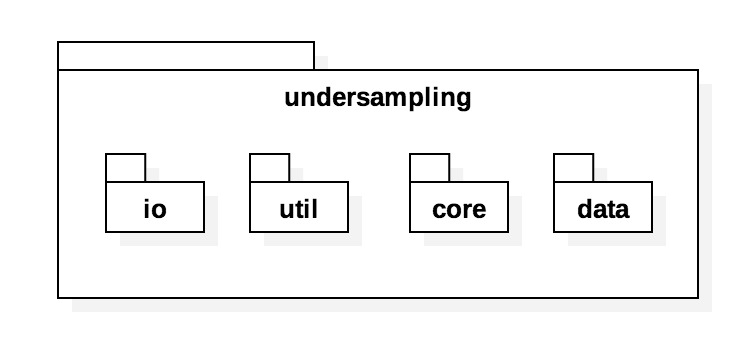
\includegraphics[width=0.80\linewidth]{./imagenes/3_paquetes.jpg}
\end{figure}

Tras diseñar los paquetes a usar, diseñé las clases que iba a necesitar para el proyecto. La estructura es bastante sencilla. Los algoritmos están implementados cada uno en su clase y todas ellas heredan de \textit{Algorithm}. Los algoritmos usan algunas funciones definidas en la clase \textit{Utilities} y usan un valor del enumerado \textit{Distances} para indicar la distancia a usar. Todos los algoritmos hacen uso de la estructura de datos representada por la clase \textit{Data}. A continuación podemos ver el diagrama de clases implementado:

\begin{figure}[H]
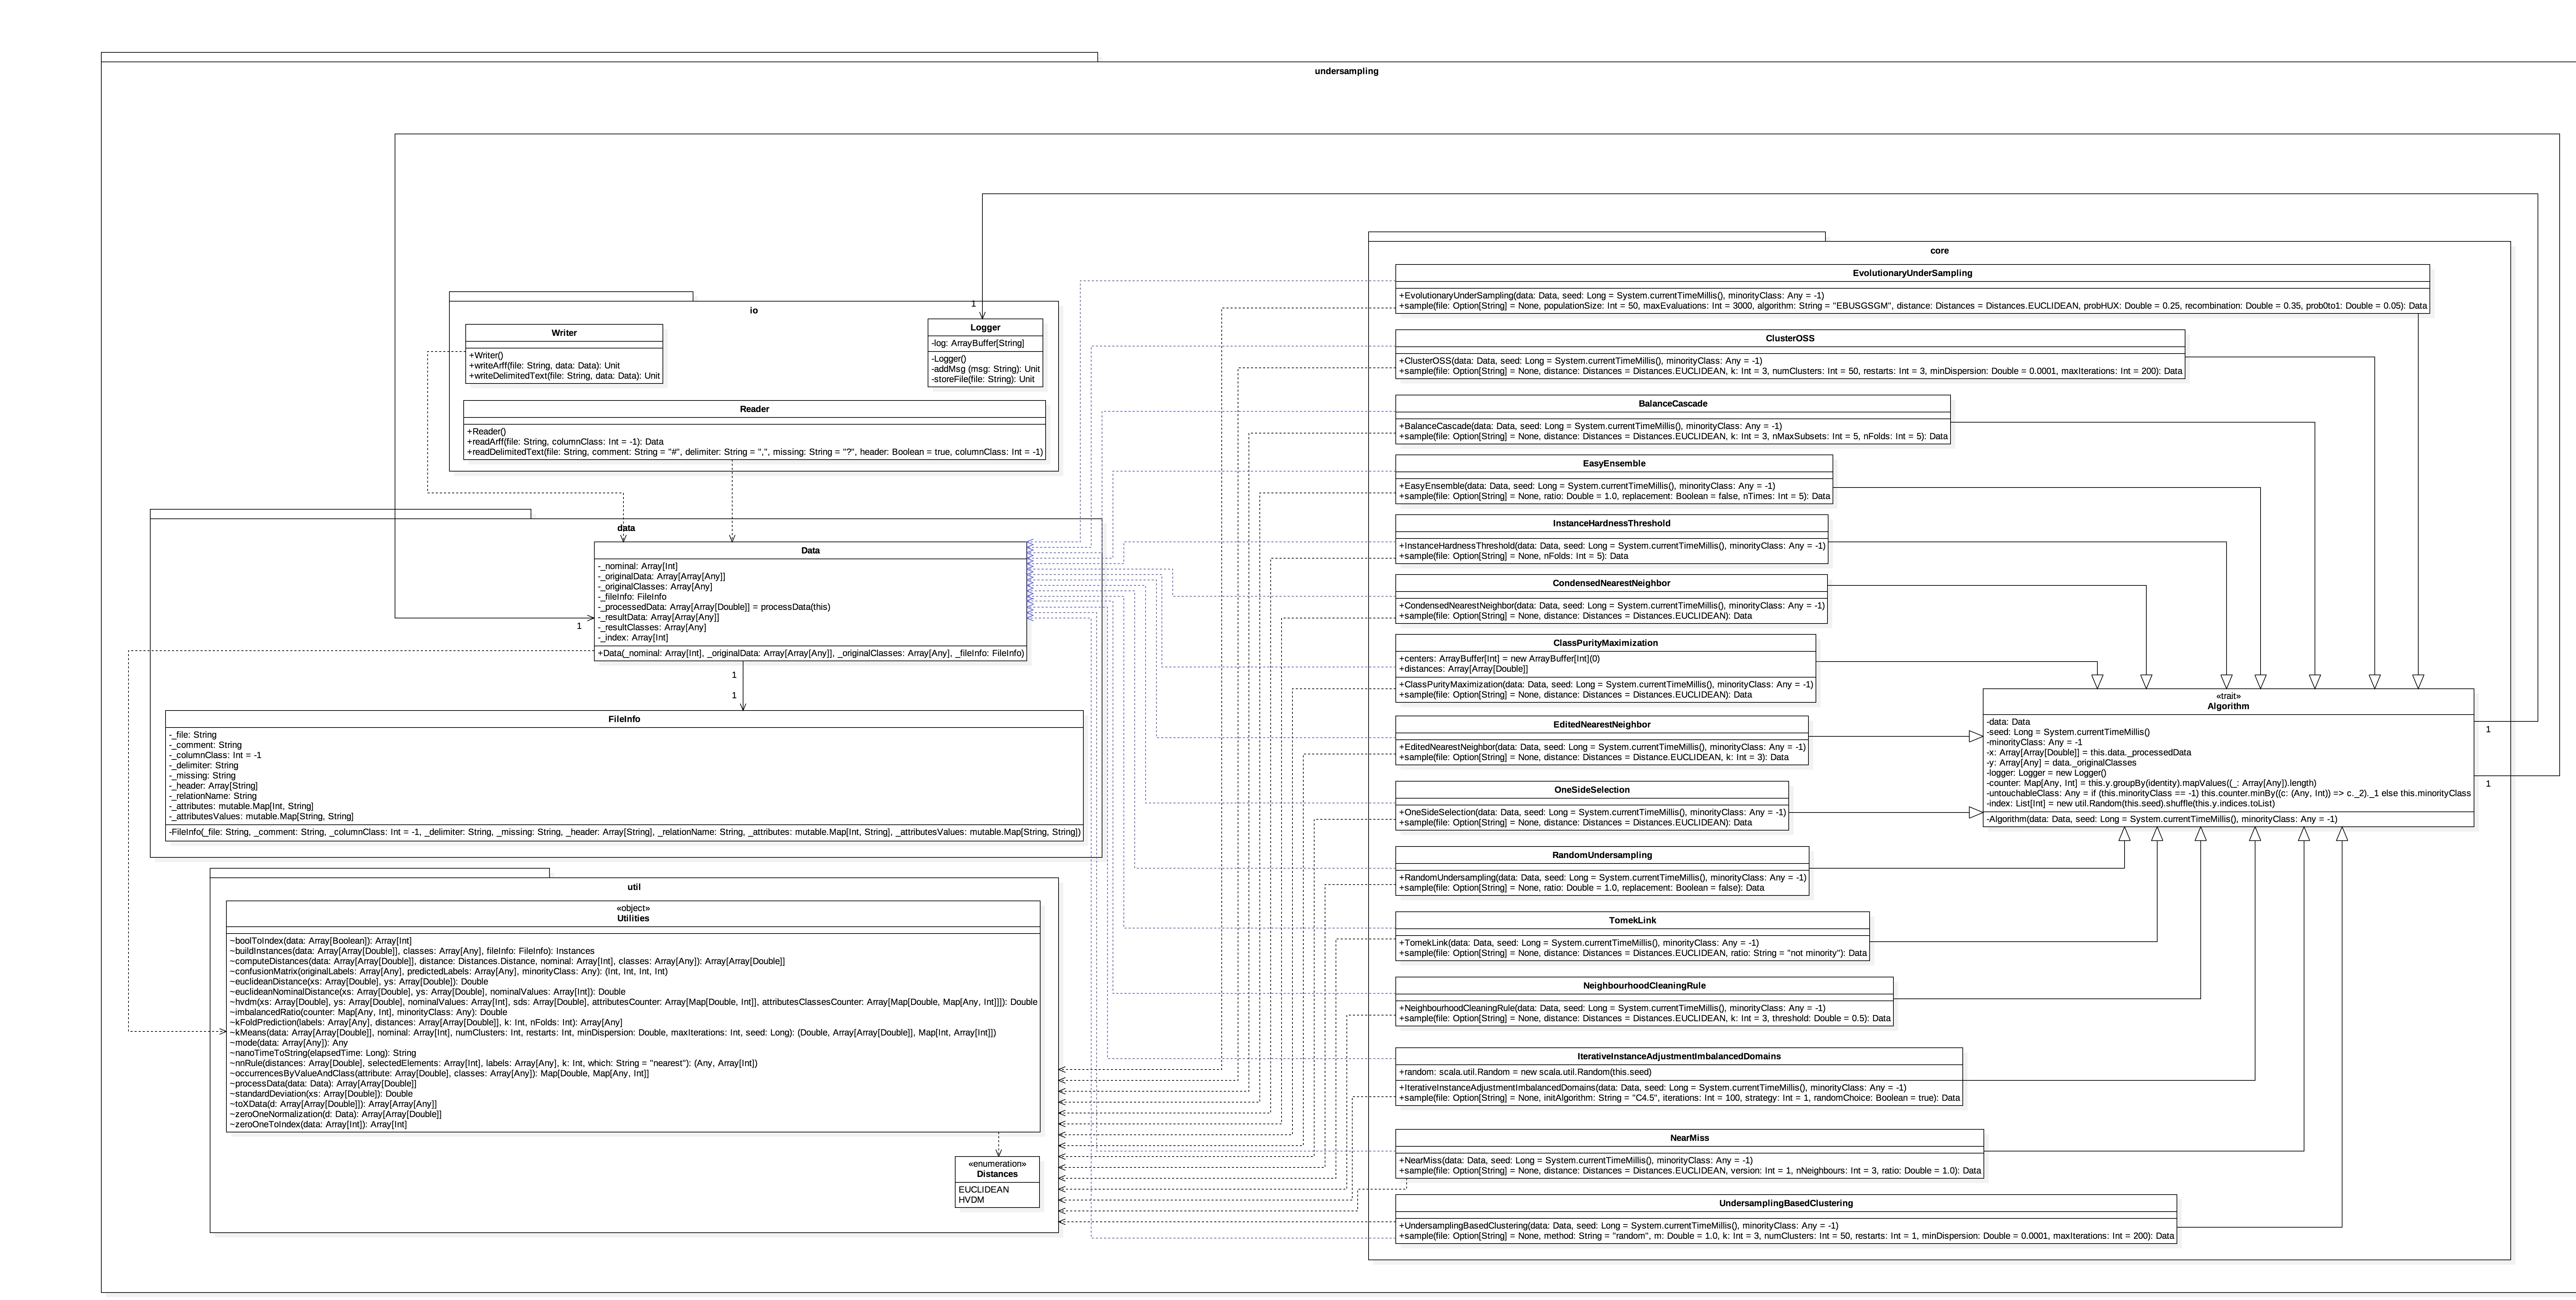
\includegraphics[scale=0.08, angle=90]{./imagenes/3_clases.jpg}
\end{figure}

Dado que no se puede ver con claridad cada clase, en la siguiente figura podemos ver un diagrama de clases simplificado, es decir, sin los métodos ni atributos de cada clase:

\begin{figure}[H]
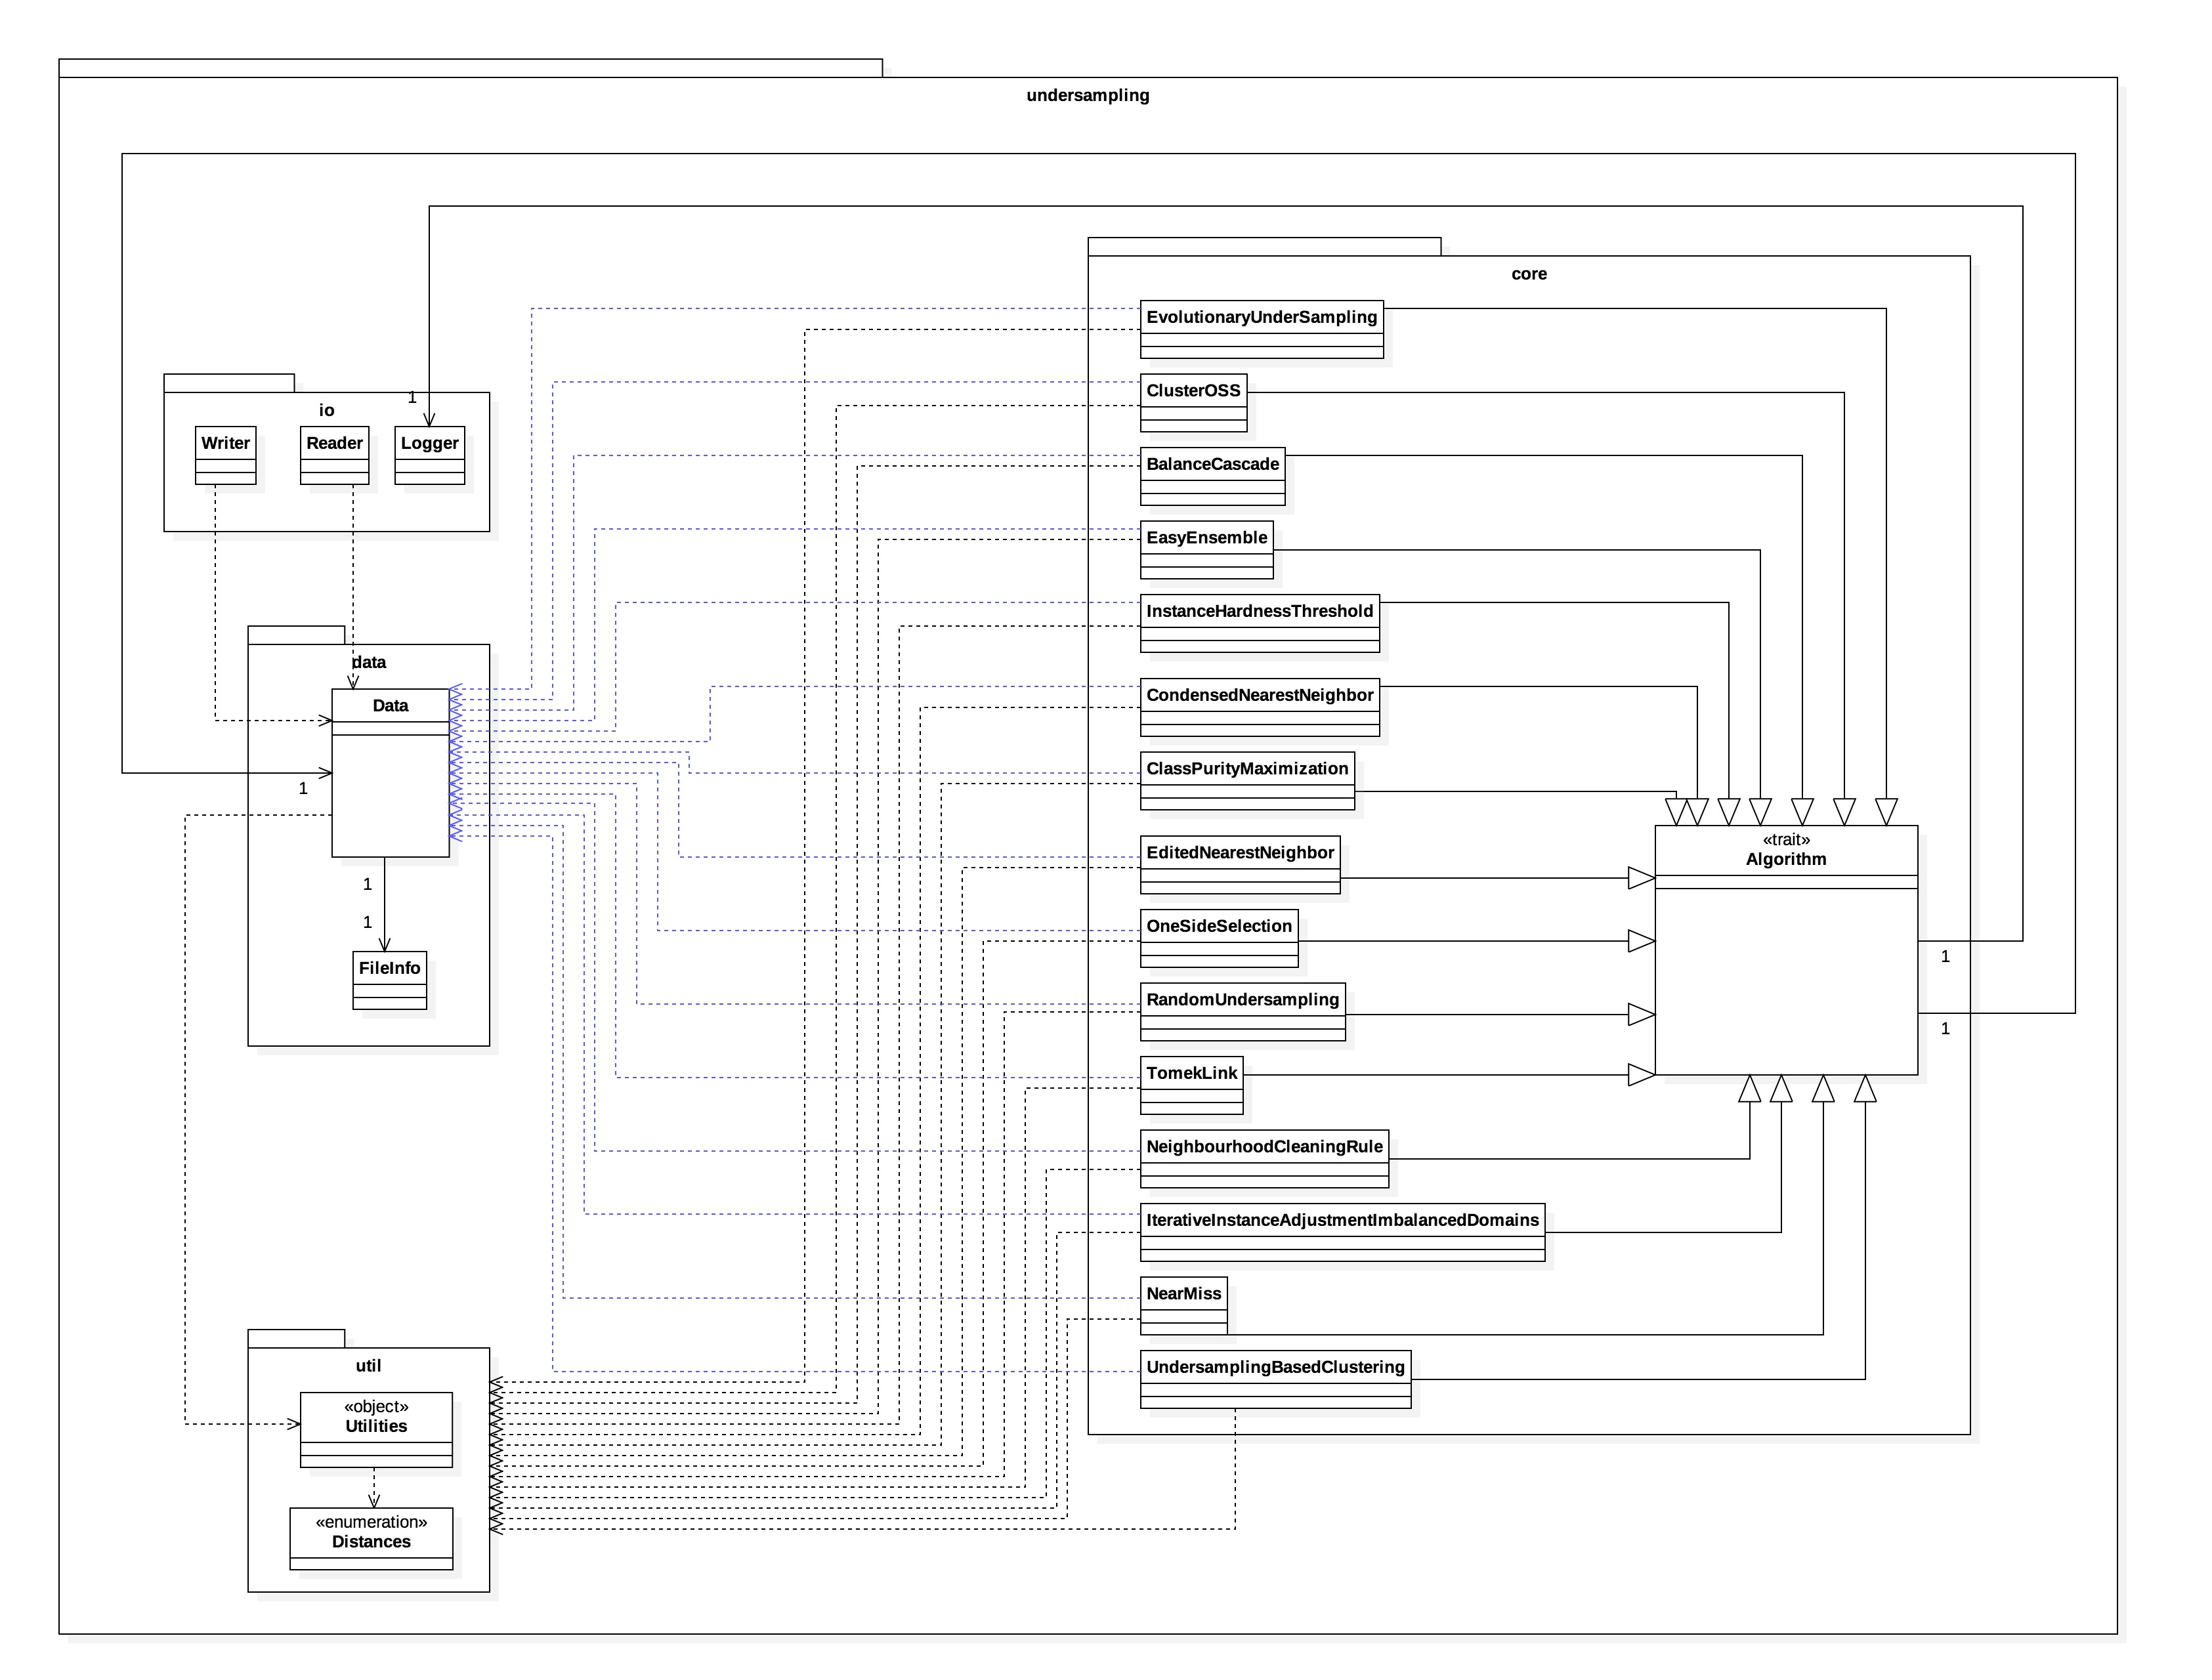
\includegraphics[scale=0.14, angle=90]{./imagenes/3_clases_simplificado.jpg}
\end{figure}

Para poder apreciar los detalles de cada clase, podemos ver las siguientes figuras:

\begin{figure}[H]
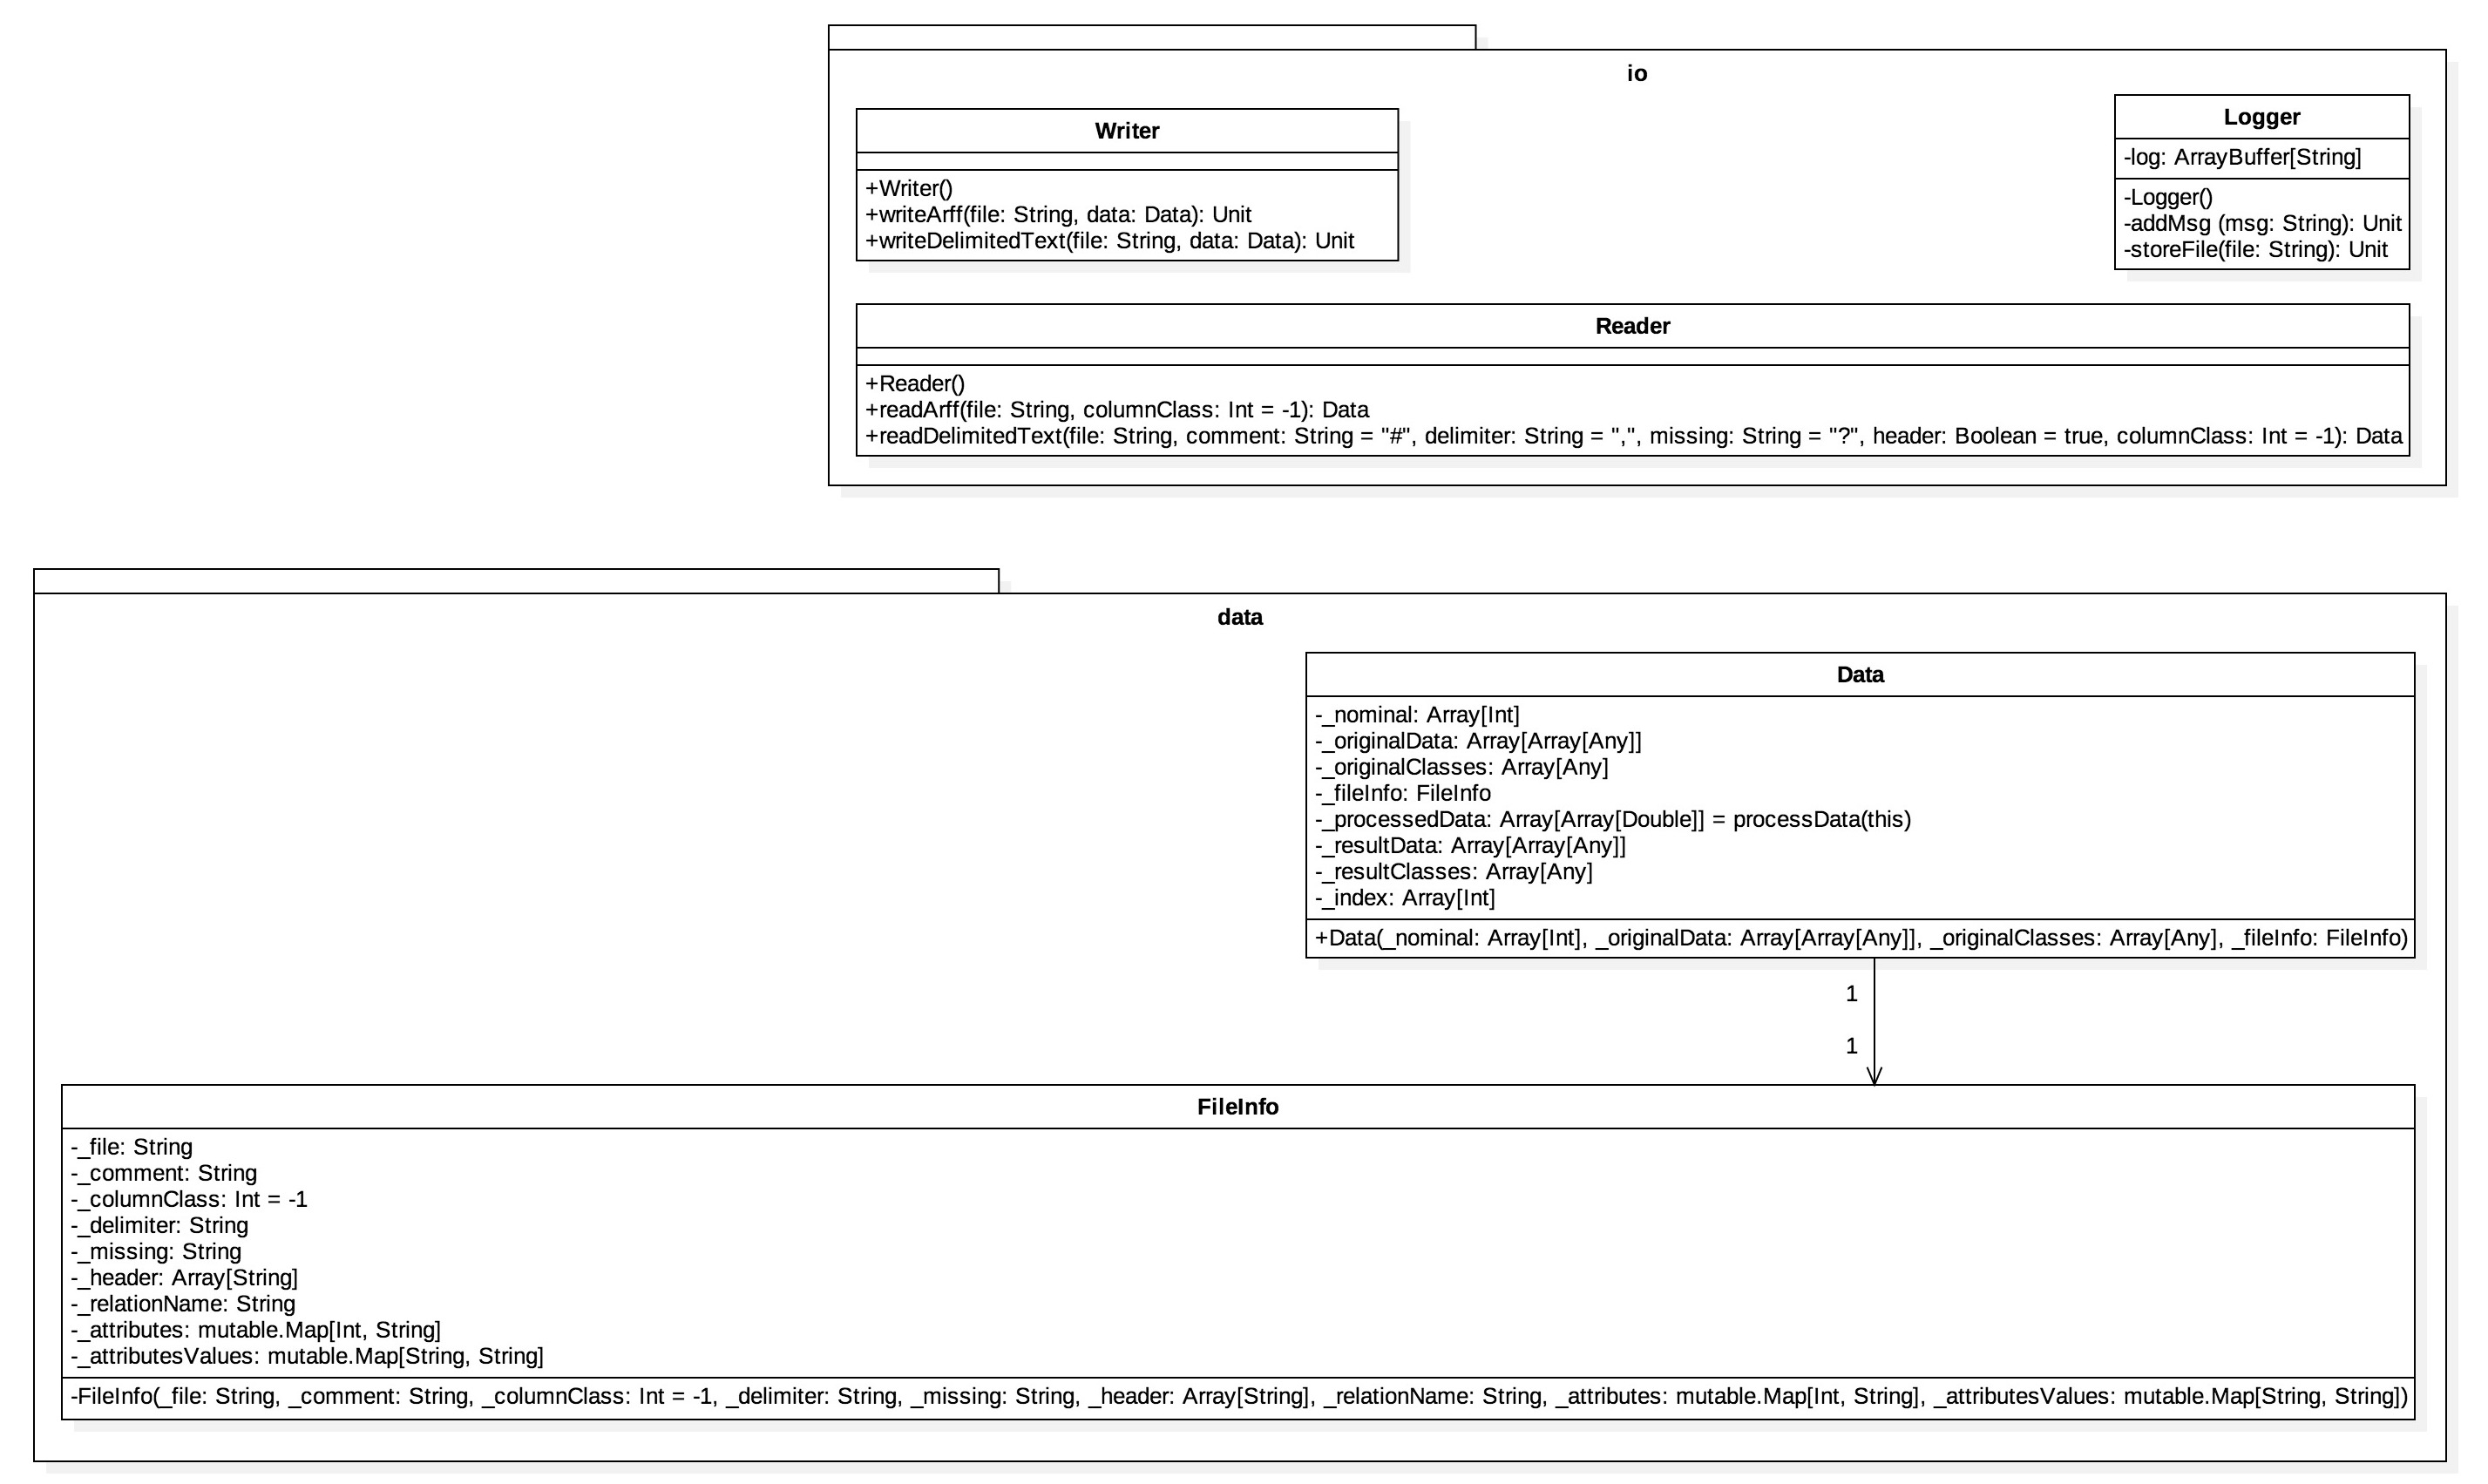
\includegraphics[scale=0.2, angle=90]{./imagenes/3_clases_detalles_pt1.jpg}
\end{figure}

\begin{figure}[H]
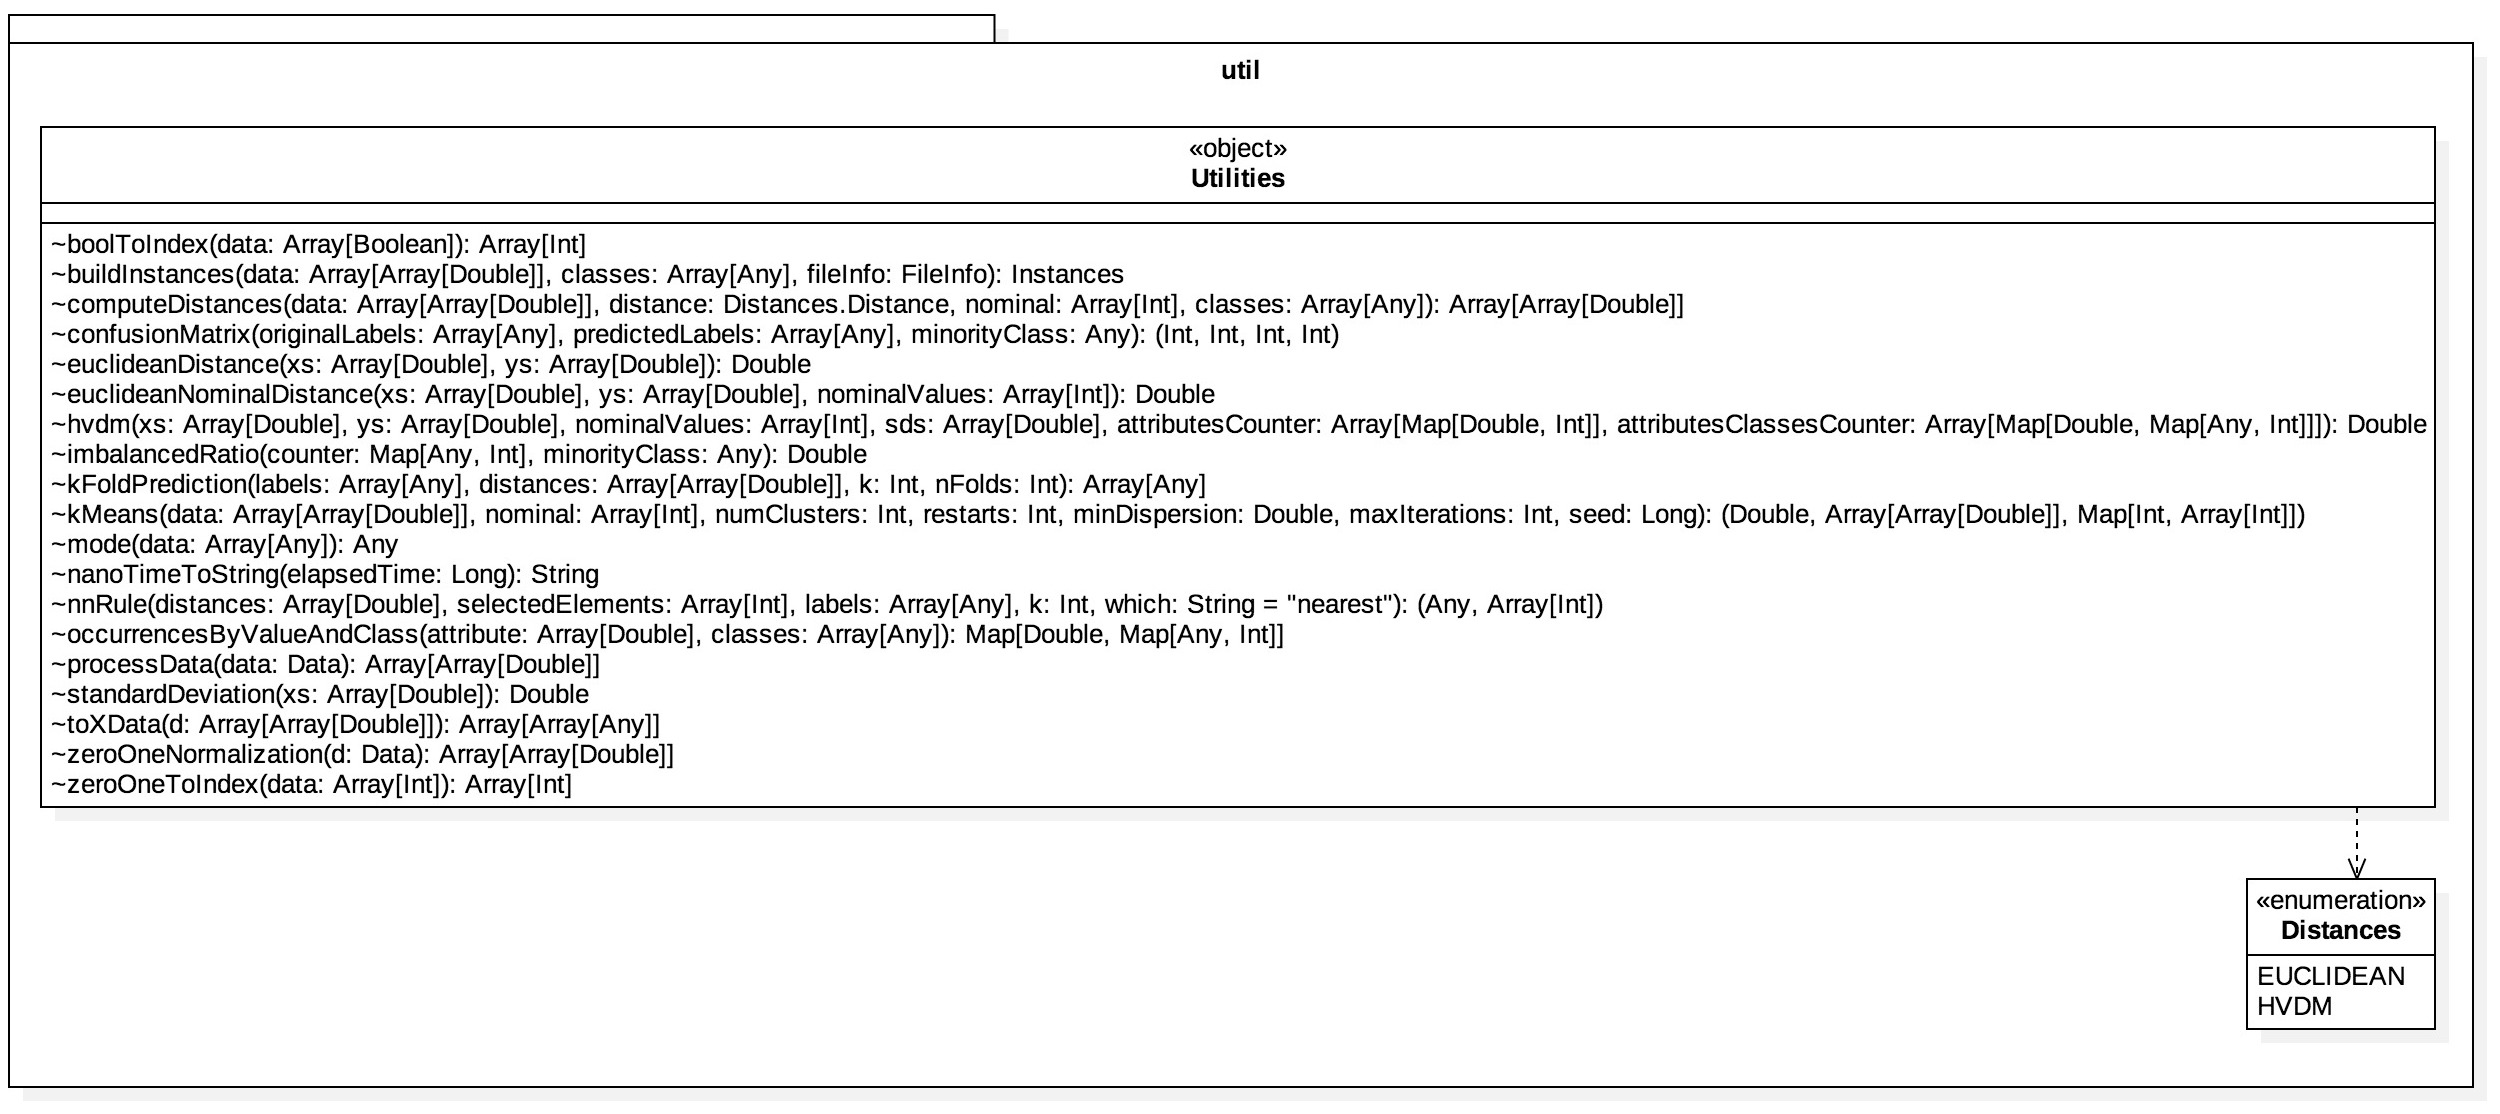
\includegraphics[scale=0.23, angle=90]{./imagenes/3_clases_detalles_pt2.jpg}
\end{figure}

\begin{figure}[H]
\centering
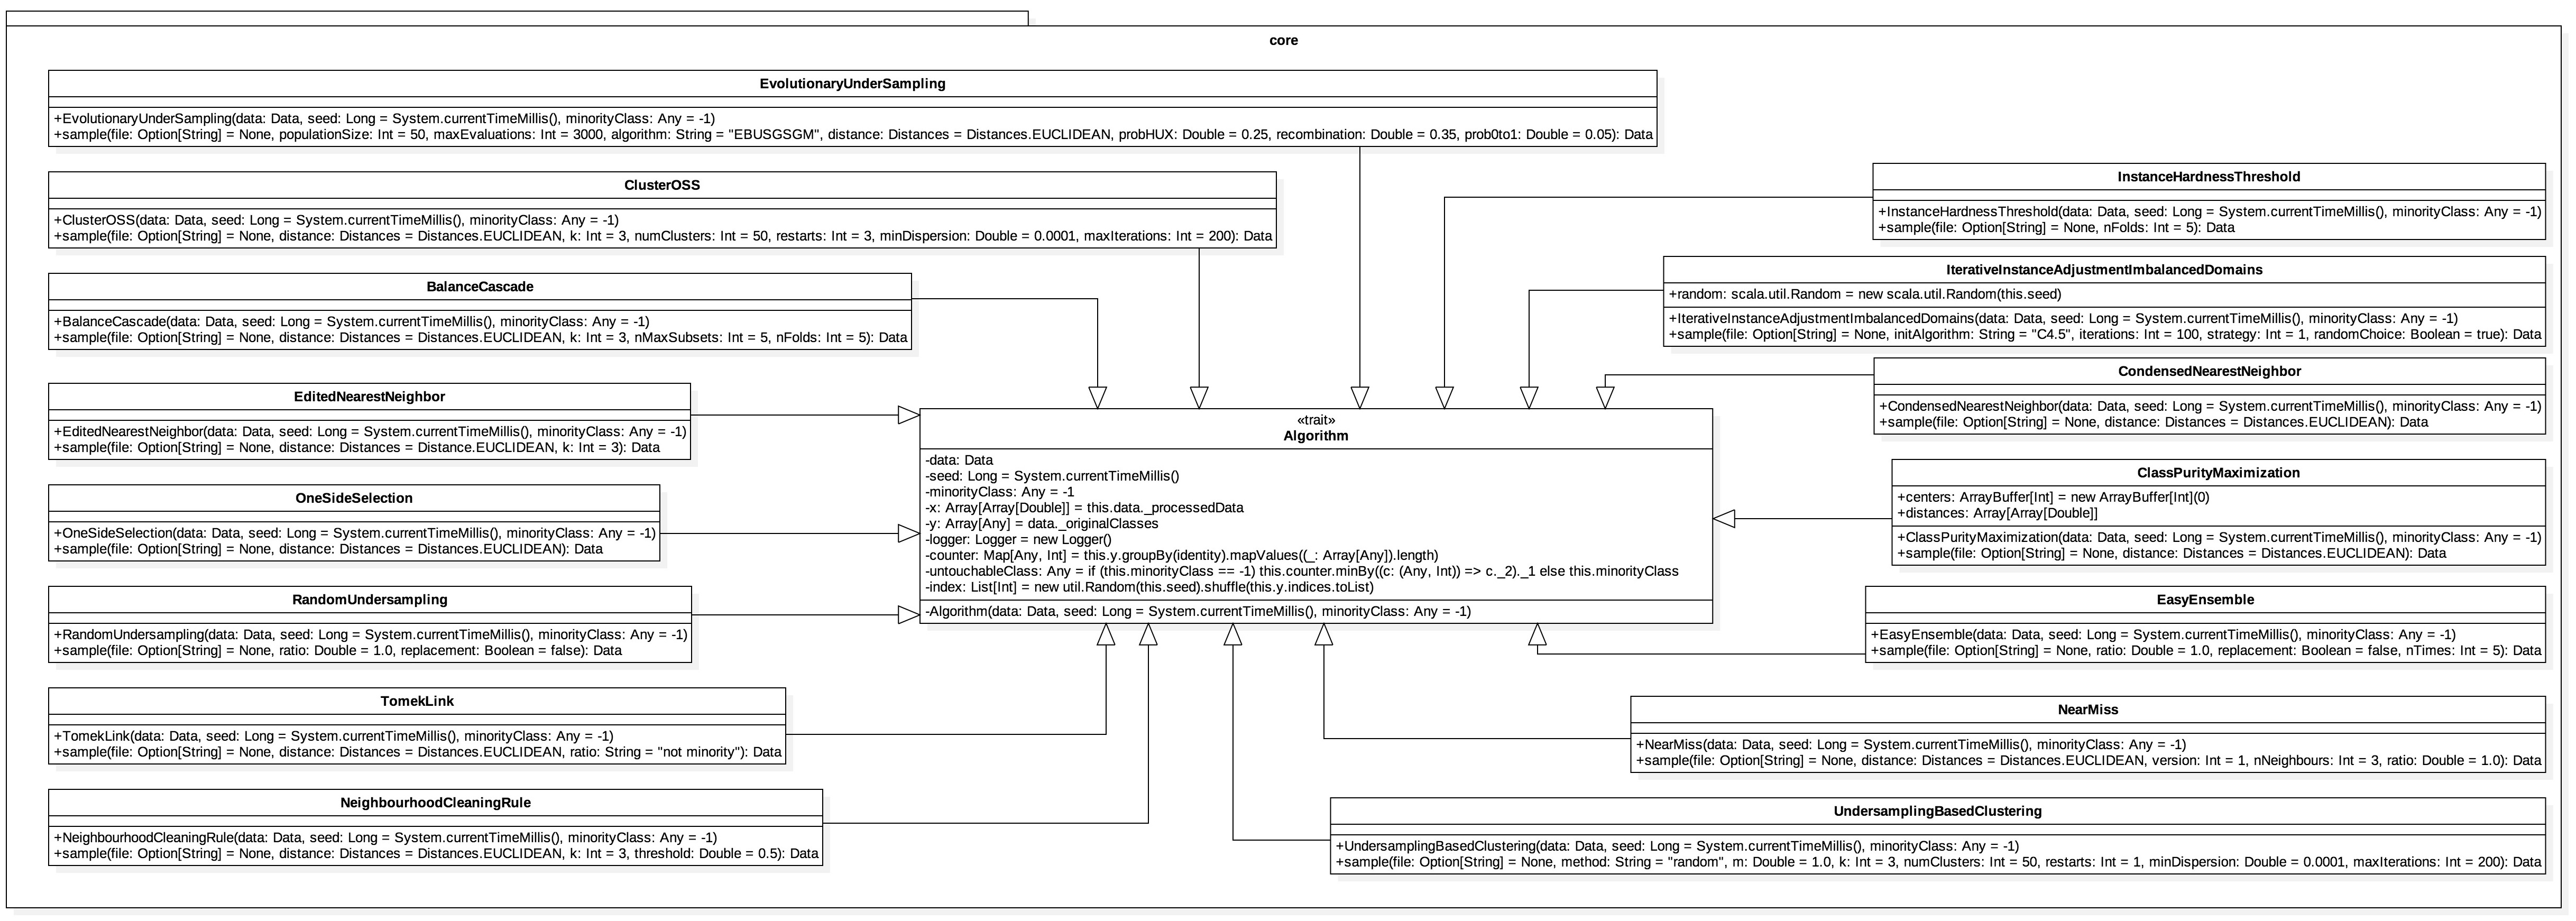
\includegraphics[scale=0.13, angle=90]{./imagenes/3_clases_detalles_pt3.jpg}
\end{figure}

\section{Presupuesto.} \label{sec:presupuesto}

Para la implementación de este proyecto se hubiese necesitado un presupuesto más o menos básico:

\begin{itemize}
	\item \textit{Un ordenador para desarrollo:} en mi caso se ha utilizado un \textit{MacBook Pro} del fabricante \textit{Apple} valorado en \textit{3300 euros}. Este es mi ordenador personal y por eso lo he usado, pero no sería necesario un ordenador tan potente. Un ordenador con un sistema \textit{Unix} y un procesador medianamente en condiciones hubiese sido suficiente, reduciendo el coste a unos \textit{800-1000 euros}.
	\item \textit{Conexión a Internet:} recurso indispensable para acceder a la documentación de \textit{Scala} y los \textit{papers} de los artículos. Dado que no se hacen grandes transferencias de datos, tampoco es necesario una conexión de gran velocidad. En mi caso se ha usado una conexión de fibra óptima de \textit{50Mb} con un precio de unos \textit{30 euros} al mes.
	\item \textit{Suministro eléctrico:} necesario para poder alimentar el ordenador. Dado que se trata de una biblioteca que maneja grande volúmenes de datos se hace un uso intenso del procesador, lo cual supone un alto consumo de batería y por tanto eléctrico.
	\item \textit{Salario:} estimo haber echado unas 350 horas en realizar todo el proyecto, incluyendo todas las partes del mismo. Supongamos que se pagan a diez euros la hora, el dinero necesario rondaría los tres mil quinientos euros.
\end{itemize}

\section{Requisitos funcionales.} \label{sec:requisitos}

Para que se trate de una biblioteca competitiva debe cumplir los siguiente requisitos:

\begin{itemize}
	\item \textit{Alta velocidad de procesamiento:} se trata de una biblioteca que puede manejar grandes volúmenes de datos. Si para conjuntos pequeños el tiempo de ejecución es elevado, este será enorme cuando se introduzca mayor volumen de datos.
	\item \textit{Diferentes formatos de entrada:} hoy en día los datos pueden venir de distintos origines y, por lo tanto, debemos estar preparados para leer una gran variedad de formatos. Esta biblioteca es capaz de leer datos en formato \textit{ARFF} \cite{arffwiki} de \textit{Weka} \cite{weka} \cite{wekaweb} y datos en cualquier formato de texto plano indicando los tokens necesarios, como puede ser el separados de elementos, el token de comentario, el token que representa valores nulos, \textit{etcetera}.
	\item \textit{Diferentes formatos de salida:} al igual que sucede con la entrada de datos, sucede con los datos de salida. Esta biblioteca permite los mismos formatos de salida que de entrada, facilitando así al usuario la posibilidad de tener el resultado de los algoritmos en el mismo formato de entrada —u otro a elegir—.
	\item \textit{Seguro a errores:} este tipo de algoritmos tiene una gran variedad de parámetros y, por lo tanto, distintas configuraciones que el usuario puede elegir. Todos los algoritmos están probados con distintos valores de estos parámetros y los propios algoritmos comprueban que los argumentos son válidos. 
	\item \textit{Datos intactos:} los datos de entrada son modificados en la mayoría de los algoritmos para poder trabajar con ellos, pero no nos podemos permitir devolver los datos modificados, ya que esos no son los datos que ha introducido el usuario. Para evitar esto, todos los algoritmos —con excepción del algoritmo \textit{IPADE-ID} ya que crea nuevos datos sintéticos y, por lo tanto, no es posible garantizar esta condición— trabajan con índices a los datos en vez de con los propios datos, para así no poder devolver los datos originales accediendo a las posiciones indicadas por el índice. Esto también nos proporciona una mayor velocidad de procesamiento, ya que es más eficiente trabajar con una colección de índices que con una matriz de \textit{n $\times$ m} elementos.
\end{itemize}
\chapter{Algoritmos seleccionados.} \label{ch:algoritmos}

En este proyecto se han implementado los siguientes 15 algoritmos: 

\begin{itemize}
	\item \textbf{Balance Cascade}, al cual nos referiremos como \textit{BC}.
	\item \textbf{Class Purity Maximization algorithm}, al cual nos referiremos como \textit{CPM}.
	\item \textbf{ClusterOSS}, al cual nos referiremos como \textit{ClusterOSS}.
	\item \textbf{Condensed Nearest Neighbor decision rule}, al cual nos referiremos como \textit{CNN}.
	\item \textbf{Easy Ensemble}, al cual nos referiremos como \textit{EE}.
	\item \textbf{Edited Nearest Neighbour rule}, al cual nos referiremos como \textit{ENN}.
	\item \textbf{Evolutionary Undersampling}, al cual nos referiremos como \textit{EUS}.
	\item \textbf{Instance Hardness Threshold}, al cual nos referiremos como \textit{IHTS}.
	\item \textbf{Iterative Instance Adjustment for Imbalanced Domains}, al cual nos referiremos como \textit{IPADE-ID}.
	\item \textbf{NearMiss}, al cual nos referiremos como \textit{NM}.
	\item \textbf{Neighbourhood Cleaning Rule}, al cual nos referiremos como \textit{NCL}.
	\item \textbf{One-Side Selection}, al cual nos referiremos como \textit{OSS}.
	\item \textbf{Random Undersampling}, al cual nos referiremos como \textit{RU}.
	\item \textbf{Tomek Link}, al cual nos referiremos como \textit{TL}.
	\item \textbf{Undersampling Based on Clustering}, al cual nos referiremos como \textit{SCB}.
\end{itemize}

En este capítulo vamos a ver el pseudocódigo de cada uno de ellos y explicar un poco su funcionamiento e idea principal.

\section{Balance Cascade.} \label{sec:alg_bc}
El artículo original donde se ha publicado este algoritmo es \textit{``Exploratory Undersampling for Class-Imbalance Learning} escrito por \textit{Xu-Ying Liu, Jianxin Wu y Zhi-Hua Zhou''} \cite{bc-ee}. El pseudocódigo del algoritmo es el siguiente:

\begin{codigo}
\begin{algorithmic}[1]
\Function {BalanceCascade}{Conjunto de instancias minoritaria P, conjuntos de instancias mayoritarias N con $\left | P \right | < \left | N \right |$, numero de subconjuntos T a crear de N, número de iteraciones de AdaBoost $s_i$}
\State \parbox[t]{305pt}{$i \leftarrow 0, f \leftarrow \sqrt[T-1]{\frac{\left | P \right |}{\left | N \right |}}$, f es el ratio de falsos positivos que H$_i$ debe alcanzar\strut}
\While{i != T}
\State i $\leftarrow$ i + 1
\State Coger de forma aleatoria un subconjunto N$_i$ con $\left | P \right | < \left | N_i \right |$
\State \parbox[t]{305pt}{Aprender H$_i$ con P, N$_i$ donde H$_i$ es un clasificador AdaBoost con s$_i$ clasificadores debiles h$_{i, j}$ y correspondientes pesos $\alpha_{i, j}$. El umbral es $\theta_i$. $H_i = sgn(\sum_{j=1}^{s_i} \alpha_{i, j} h_{i, j}(x) - \theta_i)$\strut}
\State Ajustar $\theta_i$ para que el ratio de falsos positivos de H$_i$ sea f.
\State \parbox[t]{305pt}{Quitar de N todos los ejemplos que son clasificados correctamente por H$_i$\strut}
\EndWhile
\State \Return Un conjunto: $H(x) = sgn(\sum_{i=1}^{T} \sum_{j=1}^{s_i} \alpha_{i, j} h_{i, j}(x) - \sum_{i=1}^{T} \theta_i)$
\EndFunction 
\end{algorithmic}
\end{codigo}

La idea de este algoritmo es realizar distintas particiones del conjunto de datos inicial y aprender un clasificador para cada uno de ellos y luego combinar las mejores instancias de cada subconjunto para formar el conjunto final de datos.

\section{Class Purity Maximization algorithm.} \label{sec:alg_cpm}
El artículo original donde se ha publicado este algoritmo es \textit{``An Unsupervised Learning Approach to Resolving the Data Imbalanced Issue in Supervised Learning Problems in Functional Genomics} escrito por \textit{Kihoon Yoon y Stephen Kwek''} \cite{cpm}. El pseudocódigo del algoritmo es el siguiente:

\begin{codigo}
\begin{algorithmic}[1]
\Function {ClassPurityMaximization}{}
\State \parbox[t]{305pt}{Seleccionar como centros una instancia de la clase minoritaria y otra de la clase mayoritaria\strut}
\algstore{break}
\end{algorithmic}
\end{codigo}
	
\begin{codigo}
\begin{algorithmic}[1]
\algrestore{break}
\State \parbox[t]{305pt}{Repartir el resto de instancias en cada uno de los \textit{clúster} generados en el paso dos según su cercanía a cada uno de los centros. Se debe garantizar que uno de los dos \textit{clúster} tiene un mayor valor de pureza\strut}
\State \parbox[t]{305pt}{Repetir el proceso recursivamente —en cada uno de los \textit{clúster} generados en el paso anterior— hasta que no se pueda generar una partición en la cual uno de los \textit{subclúster} tenga mayor pureza que su \textit{clúster} padre\strut}
\State \parbox[t]{305pt}{\Return Añadimos todas las instancias minoritarias a cada \textit{clúster} no puro\strut}
\EndFunction 
\end{algorithmic}
\end{codigo}

La idea de este algoritmo es ir partiendo el conjunto de datos en \textit{clústeres} e ir realizando el particionamiento mientras obtengamos un conjunto más puro —mejor— que el anterior.

\section{ClusterOSS.} \label{sec:alg_clusteross}
El artículo original donde se ha publicado este algoritmo es \textit{``ClusterOSS: a new undersampling method for imbalanced learning.''} escrito por \textit{Victor H Barella, Eduardo P Costa y André C. P. L. F. Carvalho} \cite{clusteross}. El pseudocódigo del algoritmo es el siguiente:

\begin{codigo}
\begin{algorithmic}[1]
\Function {ClusterOSS}{Conjunto de datos D}
\State \parbox[t]{305pt}{Train = $\left \{ \right \}$ Test = $\left \{ \right \}$\strut}
\State \parbox[t]{305pt}{InstanciasMayoritatias = cogerInstanciasMayoritarias(D)\strut}
\State \parbox[t]{305pt}{C = AlgClustering(InstanciasMayoritarias)\strut}
\For{$cluster\ C_i \in C$}
\State x = InstanciaMasCercanaAlCentro(C$_i$)
\State Train = Train $\cup$ $\left \{ x \right \}$
\State Test = Test $\cup\ (C_i\left \{ x \right \})$
\EndFor
\State Resultado = KNN(Train, Test)
\State MalClasificados = ObtenerMalClasificados(Resultado)
\State NuevoD = Train $\cup$ MalClasificados
\State TLinks = TomekLinks(NuevoD)
\For{z $\in$ NuevoD}
\If{z $\in$ TLinks}
\State NuevoD = NuevoD - $\left \{ z \right \}$
\EndIf
\EndFor
\State \Return NuevoD
\EndFunction 
\end{algorithmic}
\end{codigo}

\textit{AlgClustering} es una función que aplica un algoritmo de \textit{clustering}. En este proyecto se ha usado \textit{kMeans} \cite{kmeans}. \\ 

La idea de este algoritmo es construir varios \textit{clústeres} para quedarnos con los elementos más representativos del conjunto de datos original. Una vez tenemos los elementos más representativos, aplicamos un algoritmo \textit{Tomek Link} —el cual podemos ver en la sección \ref{sec:alg_tl}— para limpiar elementos ruidosos.

\section{Condensed Nearest Neighbor decision rule.} \label{sec:alg_cnn}
El artículo original donde se ha publicado este algoritmo es \textit{``The Condensed Nearest Neighbor Rule''} escrito por \textit{P. Hart} \cite{cnn}. El pseudocódigo del algoritmo es el siguiente:

\begin{codigo}
\begin{algorithmic}[1]
\Function {CNN}{}
\State El primer ejemplo se coloca en \textit{STORE}
\State \parbox[t]{305pt}{El segundo ejemplo se clasifica usando la regla NN usando como conjunto de datos el contenido de \textit{STORE}. Si se clasifica correctamente, dicho ejemplo se mete en \textit{GRABBAG}, en caso contrario se pone en \textit{STORE}\strut}
\State \parbox[t]{305pt}{De forma iterativa, se repite el proceso del paso 2 para cada ejemplo restante\strut} 
\State \parbox[t]{305pt}{Tras una primera pasada por los datos, se procede a iterar sobre \textit{GRABBAG} hasta terminar, lo cual puede suceder por:\strut} 
\begin{itemize}
	\item \parbox[t]{305pt}{Todos los elementos de \textit{GRABBAG} se han transferido a \textit{STORE}. En este caso, el conjunto obtenido es igual que el original\strut}
	\item \parbox[t]{305pt}{Se ha realizado una pasada entera sobre \textit{GRABBAG} y ningún elemento ha sido transferido a \textit{STORE}\strut}
\end{itemize}
\State \Return El contenido de \textit{STORE} es el resultado final
\EndFunction 
\end{algorithmic}
\end{codigo}

La idea de este algoritmo es bien sencilla. Busca eliminar puntos innecesarios. Un punto se considera innecesario si con el conjunto de puntos que llevamos guardados hasta el momento somos capaces de predecir correctamente su clase. Si esto es así, no nos interesa ese punto y lo descartamos.

\section{Easy Ensemble.} \label{sec:alg_ee}
El artículo original donde se ha publicado este algoritmo es \textit{``Exploratory Undersampling for Class-Imbalance Learning''} escrito por \textit{Xu-Ying Liu, Jianxin Wu y Zhi-Hua Zhou} \cite{bc-ee}. El pseudocódigo del algoritmo es el siguiente:

\begin{codigo}
\begin{algorithmic}[1]
\Function {EasyEnsemble}{Conjunto de instancias minoritaria P, conjuntos de instancias mayoritarias N con $\left | P \right | < \left | N \right |$, numero de subconjuntos T a crear de N, número de iteraciones de AdaBoost $s_i$}
\State $i \leftarrow 0$
\While{i != T}
\State i $\leftarrow$ i + 1
\State Coger de forma aleatoria un subconjunto N$_i$ con $\left | P \right | < \left | N_i \right |$
\State \parbox[t]{305pt}{Aprender H$_i$ con P, N$_i$ donde H$_i$ es un clasificador AdaBoost con s$_i$ clasificadores debiles h$_{i, j}$ y correspondientes pesos $\alpha_{i, j}$. El umbral es $\theta_i$. $H_i = sgn(\sum_{j=1}^{s_i} \alpha_{i, j} h_{i, j}(x) - \theta_i)$\strut}
\EndWhile
\State \Return Un conjunto: $H(x) = sgn(\sum_{i=1}^{T} \sum_{j=1}^{s_i} \alpha_{i, j} h_{i, j}(x) - \sum_{i=1}^{T} \theta_i)$
\EndFunction 
\end{algorithmic}
\end{codigo}

Este algoritmo sigue la misma idea que \textit{BC} \ref{sec:alg_bc}. Busca realizar distintas particiones del conjunto de datos inicial y aprender un clasificador para cada uno de ellos y luego combinar las mejores instancias de cada subconjunto para formar el conjunto final de datos.

\section{Edited Nearest Neighbour rule.} \label{sec:alg_enn}
El artículo original donde se ha publicado este algoritmo es \textit{``Asymptotic Properties of Nearest Neighbor Rules Using Edited Data''} escrito por \textit{Dennis L. Wilson} \cite{enn}. El pseudocódigo del algoritmo es el siguiente:

\begin{codigo}
\begin{algorithmic}[1]
\Function {ENN}{Conjunto de datos D}
\State S = D
\For{x$_i \in$ S}
\State \parbox[t]{305pt}{Descartamos x$_i$ de S si no se clasifica correctamente usando la relga NN usando como conjunto de datos D - $\left \{ x_i \right \}$\strut}
\EndFor
\State \Return S
\EndFunction 
\end{algorithmic}
\end{codigo}

La idea de este algoritmo es bastante similar a la de \textit{CNN} \ref{sec:alg_cnn}, va eliminando puntos del conjunto de datos si se consideran redundantes, es decir, podemos predecir su clase usando todos los puntos del conjunto original quitando el que estamos tratando.

\section{Evolutionary Undersampling.} \label{sec:alg_eus}
El artículo original donde se ha publicado este algoritmo es \textit{``Evolutionary Under-Sampling for Classification with Imbalanced Data Sets: Proposals y Taxonomy''} escrito por \textit{Salvador Garcia y Francisco Herrera} \cite{eus}. El pseudocódigo de este algoritmo es el pseudocódigo de cualquier algoritmo evolutivo, el cuál es el siguiente:

\begin{codigo}
\begin{algorithmic}[1]
\Function {EUS}{Conjunto de datos D}
\State Generar población aleatoria inicial
\While{numeroEvaluaciones $<$ evaluacionesMaximas}
\State \parbox[t]{305pt}{Generamos los nuevos descendientes a partir de la población actual\strut}
\State \parbox[t]{305pt}{Evaluamos los nuevos descendientes\strut}
\State \parbox[t]{305pt}{Ordenamos la población actual y la nueva población\strut}
\State \parbox[t]{305pt}{Mezclamos las dos poblaciones quedándonos con los N mejores individuos, donde N es el tamaño original de la población.\strut}
\EndWhile
\State \Return El mejor individuo de la población
\EndFunction 
\end{algorithmic}
\end{codigo}

Dado que es un algoritmos evolutivo, podemos describir las características principales del mismo:

\begin{itemize}
	\item \textit{Representación del individuo}: cada individuo es un vector de tamaño $\left | conjunto\_original \right |$ formado por unos y/o ceros. Cada individuo representa un subconjunto de elementos del conjunto original. Si en la posición \textit{i} del vector hay un uno, la instancia \textit{i} está incluida en dicho subconjunto.
	\item \textit{Población inicial:} población aleatoria formada por el número de individuos indicado por el usuario.
	\item \textit{Función de evaluación:} este algoritmo admite distintas funciones de evaluación según la versión deseada a ejecutar.
	\begin{itemize}
		\item Para la versión \textit{EBUSGSGM} se usa
		\begin{equation}
			g - abs(1 - (nPositives / nNegatives)) * 20
		\end{equation}
		 donde \textit{g} es la media geométrica —la cual podemos ver explicada con detalle en la subsección \ref{subsec:gm}—, \textit{nPositives} es el número de instancias positivas en el subconjunto seleccionado y \textit{nNegatives} es el número de instancias negativas en el subconjunto seleccionado.
		\item Para la versión \textit{EBUSMSGM} se usa
		\begin{equation}
			g - abs(1 - (nPositivesTotal / nNegatives)) * 20
		\end{equation}
		donde \textit{g} es la media geométrica, \textit{nPositivesTotal} es el número de instancias positivas en el conjunto original y \textit{nNegatives} es el número de instancias negativas en el subconjunto seleccionado.
		\item Para la versión \textit{EUSCMGSGM} se usa la media geométrica.
		\item Para la versión \textit{EUSCMMSGM} se usa la media geométrica.
		\item Para la versión \textit{EBUSGSAUC} se usa
		\begin{equation}
			auc - abs(1 - (nPositives / nNegatives)) * 0.2	
		\end{equation} 
		donde \textit{auc} es el área bajo la curva \textit{ROC} —la cual podemos ver explicada con detalle en la subsección \ref{subsec:auc}—, \textit{nPositives} es el número de instancias positivas en el subconjunto seleccionado y \textit{nNegatives} es el número de instancias negativas en el subconjunto seleccionado.
		\item Para la versión \textit{EBUSMSAUC} se usa
		\begin{equation}
			auc - abs(1 - (nPositivesTotal / nNegatives)) * 0.2
		\end{equation}
		donde \textit{auc} es el área bajo la curva \textit{ROC} \textit{nPositivesTotal} es el número de instancias positivas en el conjunto original y \textit{nNegatives} es el número de instancias negativas en el subconjunto seleccionado.
		\item Para la versión \textit{EUSCMGSAUC} se usa el área bajo la curva \textit{ROC}.
		\item Para la versión \textit{EUSCMMSAUC} se usa el área bajo la curva \textit{ROC}.
	\end{itemize}
	\item \textit{Criterio de parada:} el algoritmo acepta un parámetro mediante el cual el usuario puede indicar el número de evaluaciones límite que puede hacer el algoritmo.
	\item \textit{Operador de cruce:} se ha usado el operador de cruce \textit{HUX}. Este operador genera dos nuevo descendientes intercambiando los genes —un gen es un elemento del vector que representa al individuo— de sus dos ancestros. El intercambio se produce si la distancia \textit{Hamming} —el número de genes distintos entre los dos ancestros— es mayor que un umbral indicado por el usuario.
\end{itemize}

Las versiones cuyo nombre contiene \textit{GS} indican que se aplica \textit{Global Selection}, es decir, se pueden descartar instancias de la clase minoritaria. Las versiones cuyo nombre contiene \textit{MS} indican que se aplica \textit{Majority Selection}, es decir, sólo se pueden descartar instancias de la clase mayoritaria. \\

Las versiones cuyo nombre contiene \textit{GM} indican que se usa la media geométrica como componente principal de la función de evaluación. Las versiones cuyo nombre contiene \textit{AUC} indican que se usa el área bajo la curva \textit{ROC} como componente principal de la función de evaluación. \\

Las versiones cuyo nombre contiene \textit{EBUS} —que significa \textit{Evolutionary Balancing Under-Sampling}— priorizan obtener un conjunto de datos equilibrado. Las versiones cuyo nombre contiene \textit{EUSCM} —que significa \textit{Evolutionary Under-Sampling guided by Classification Measures}— priorizan obtener un conjunto de datos con buenos resultados a la hora de realizar clasificación, dejando en un segundo plano el objetivo de buscar un conjunto de datos equilibrado.

\section{Instance Hardness Threshold.} \label{sec:alg_ihts}
El artículo original donde se ha publicado este algoritmo es \textit{``An Empirical Study of Instance Hardness''} escrito por \textit{Michael R. Smith, Tony Martinez y Christophe Giraud-Carrier} \cite{ihts}. El pseudocódigo del algoritmo es el siguiente:

\begin{codigo}
\begin{algorithmic}[1]
\Function {IHTS}{Conjunto de datos D}
\State \parbox[t]{305pt}{Calcular $k-Disagreeing Neighbors\ - \ kDN$\strut}
\State \parbox[t]{305pt}{Calcular $Disjunct Size\ - \ DS$\strut}
\State \parbox[t]{305pt}{Calcular $Disjunct Class Percentage\ - \ DCP$\strut}
\State \parbox[t]{305pt}{Calcular $Class Likelihood\ - \ Cl$\strut}
\State \parbox[t]{305pt}{Calcular $Class Likelihood Difference\ - \ CLD$\strut}
\State \parbox[t]{305pt}{Calcular $Minority Value\ - \ MV$\strut}
\State \parbox[t]{305pt}{Calcular $Class Balance\ - \ CB$\strut}
\State \parbox[t]{305pt}{La dureza de una instancia se calcula como $0.5569 * DN - 0.1984 * DCP - 0.124 * CL + 0.0752 * CB - 0.072 * CLD + 0.0365 * DS + 0.0339 * MV + 0.9088$\strut}
\State \parbox[t]{305pt}{Clasificar las instancias según su dureza: alta si $(CLD(x,t(x)) < 0\ y\ ((DS(x) == 0\ y\ DCP(x) < 0.5)\ o\ DN(x) > 0.8))$, baja si $((DS(x) == 0\ y\ DCP(x) < 1)\ o\ DN(x) > 0.2)$ o ninguna en otro caso.\strut}
\State \parbox[t]{305pt}{Las instancias con una dureza alta se consideran que están mal clasificadas o son ruidosas y, por lo tanto, son eliminadas del conjunto de datos.\strut}
\EndFunction 
\end{algorithmic}
\end{codigo}

kDN se puede calcular de la siguiente forma: 

\begin{equation}
	kDN(x) = \frac{\left \{ y:y \in kNN(x) \wedge t(y) \neq t(x) \right \}}{k}
\end{equation}

donde \textit{kNN(x)} es el conjunto de los \textit{k} vecinos más cercanos de \textit{x} y \textit{t(x)} es la clase asociada a \textit{x}. \\

DS se puede calcular de la siguiente forma: 

\begin{equation}
	DS(x) = \frac{\left | disjunct(x) - 1 \right |}{max_{y\in D}\left | disjunct(y) - 1 \right |}
\end{equation}

donde \textit{disjunct(x)} es una función que devuelve el subconjunto de un árbol de decisión \textit{C4.5} que cubre a \textit{x}. \\

DCP se puede calcular de la siguiente forma:

\begin{equation}
	DCP(x) = \frac{\left | \left \{ z:z \in disjunct(x) \wedge t(z) = t(x) \right \} \right |}{\left | disjunct(x) \right |}
\end{equation}

donde \textit{disjunct(x)} es una función que devuelve el subconjunto de un árbol de decisión \textit{C4.5} que cubre a \textit{x} y \textit{t(x)} es la clase asociada a \textit{x}. \\

CL se puede calcular de la siguiente forma:

\begin{equation}
	CL(x, t(x)) = \prod_{i}^{\left | x \right |} P(x_i | t(x))
\end{equation}

donde \textit{x$_i$} es el valor de la instancia \textit{x} en su atributo \textit{i-ésimo}. \\

CLD es la diferencia entre CL y la máxima probabilidad para todas las otras clases. Se puede calcular de la siguiente forma:

\begin{equation}
	CLD(x, t(x)) = CL(x, t(x)) - \underset{y \in Y - t(x)}{argmax} \ CL(x, y)
\end{equation}

MV se puede calcular de la siguiente forma:

\begin{equation}
	MV(x) = \frac{\left | \left \{ z : z \in D \wedge t(z) = t(x) \right \} \right |}{max_{y\in Y} \left | \left \{ z : z \in D \wedge t(z) = y \right \} \right |}
\end{equation}

Finalmente, CB se puede calcular de la siguiente forma:

\begin{equation}
	MV(x) = \frac{\left | \left \{ z : z \in D \wedge t(z) = t(x) \right \} \right |}{\left | D \right |} - \frac{1}{\left | Y \right |}
\end{equation}

\section{Iterative Instance Adjustment for Imbalanced Domains.} \label{sec:alg_ipade_id}
El artículo original donde se ha publicado este algoritmo es \textit{``Addressing imbalanced classification with instance generation techniques: IPADE-ID''} escrito por \textit{Victoria López, Isaac Triguero, Cristóbal J. Carmona, Salvador García y Francisco Herrera} \cite{ipade}. El pseudocódigo del algoritmo es el siguiente:

\begin{codigo}
\begin{algorithmic}[1]
\Function {IPADE-ID}{Conjunto de datos D}
\State \parbox[t]{305pt}{GS = Inicializar la población usando un árbol de decisión C4.5 o kNN\strut}
\State \parbox[t]{305pt}{Mejorar la población GS aplicando un algoritmo de Evolución Diferencial\strut}
\State \parbox[t]{305pt}{AUC = evaluar población GS con TR\strut}
\State \parbox[t]{305pt}{registro de clases$\left [ 0..nClases \right ]$ = optimizable\strut}
\State \parbox[t]{305pt}{numOptim$\left [ 0..nClases \right ]$ = 0\strut}
\While{AUC != 1 quedan clases optimizables}
\State menorPrecision = $\infty$
\For{i=1 to nClases}
\If{registro de clases$\left [ i \right ]$ es optimizable}
\State \parbox[t]{305pt}{precision$\left [ i \right ]$ = Evaluar(GS, ejemplos de TR con clase i)\strut}
\If{precision$\left [ i \right ]$ $<$ menorPrecision}
\State menorPrecision = precision$\left [ i \right ]$
\State claseObj = i
\EndIf
\EndIf
\EndFor
\If{claseObj = minoritaria y numOptim$\left [ claseObj \right ] >$ 0}
\State \parbox[t]{295pt}{Mejorar la población GS$_{trial}$ aplicando un algoritmo de Evolución Diferencial\strut}
\Else
\State \parbox[t]{295pt}{GS$_{trial}$ = GS $\cup$ $\{$ ejemplos aleatorios cogidos de TR pertenecientes a la clase claseObj $\}$ \strut}
\State \parbox[t]{295pt}{Mejorar la población GS$_{trial}$ aplicando un algoritmo de Evolución Diferencial\strut}
\EndIf
\State \parbox[t]{295pt}{AUC$_{trial}$ = evaluar población GS$_{trial}$ con TR\strut}
\If{AUC$_{trial}$ $>$ AUC}
\State \parbox[t]{295pt}{AUC = AUC$_{trial}$\strut}
\State \parbox[t]{295pt}{GS = GS$_{trial}$\strut}
\State \parbox[t]{295pt}{numero de optimizaciones$\left [ i \right ]$ = 0\strut}
\Else
\If{claseObj = minoritaria y numOptim$\left [ claseObj \right ] <$ T}
\State \Comment T es el número máximo de optimizaciones
\State registro de clases$\left [ claseObj \right ]$++
\Else
\State registro de clases$\left [ claseObj \right ]$ = no optimizable
\EndIf
\EndIf
\EndWhile
\State \Return GS
\EndFunction 
\end{algorithmic}
\end{codigo}

Este algoritmo inicia la población con las instancias más relevantes del conjunto de datos original. Para obtener estas instancias seguimos los siguientes pasos:

\begin{itemize}
	\item Se aprende un árbol de decisión \textit{C4.5} con el conjunto de datos original.
	\item Se crean tantos \textit{clústeres} como nodos hoja contenga el árbol. Para cada instancia del conjunto de datos, se determina que hoja del árbol es la que clasifica dicha instancia y se añade a su correspondiente \textit{clúster}.
	\item Se calculan los centroides de cada \textit{clúster}.
	\item Para cada \textit{clúster} calculamos la instancia más cercana al centroide. El conjunto de instancias inicial es el formado por la unión de estas instancias.
\end{itemize}

Con este proceso de selección inicial nos garantizamos coger las instancias más representativas de todo el conjunto de datos. Una vez las tenemos, aplicamos de forma iterativa una versión simplificada del algoritmo \textit{Differential Evolution} \cite{differential_evolution} para mejorar el conjunto de datos obtenido en la iteración anterior. Este proceso lo hacemos hasta que no podamos mejorar el valor de la función evaluación. En este caso, la función de evaluación es el área bajo la curva \textit{ROC} —métrica que explicaremos en la subsección \ref{subsec:auc}—.

\section{NearMiss.} \label{sec:alg_nm}
El artículo original donde se ha publicado este algoritmo es \textit{``kNN Approach to Unbalanced Data Distribution: A Case Study involving Information Extraction''} escrito por \textit{Jianping Zhang y Inderjeet Mani} \cite{nm}. El pseudocódigo del algoritmo es el siguiente:

\begin{codigo}
\begin{algorithmic}[1]
\Function {NM}{}
\If{version = 1}
\State \parbox[t]{295pt}{Seleccionamos los elementos mayoritarios cuya distancia media a sus tres vecinos de la clase minoritaria más cercanos sea menor\strut}
\If{version = 2}
\State \parbox[t]{290pt}{Seleccionamos los elementos mayoritarios cuya distancia media a sus tres vecinos de la clase minoritaria más lejanos sea menor\strut}
\Else
\State \parbox[t]{290pt}{Seleccionamos de forma aleatoria una cantidad de elementos mayoritarios para cada elemento minoritario\strut}
\EndIf
\EndIf
\algstore{break}
\end{algorithmic}
\end{codigo}
	
\begin{codigo}
\begin{algorithmic}[1]
\algrestore{break}
\State \parbox[t]{305pt}{\Return Elementos minoritarios de D $\cup$ Elementos seleccionados en los pasos anteriores del algoritmo\strut}
\EndFunction 
\end{algorithmic}
\end{codigo}

La idea de este algoritmo es eliminar los vecinos mayoritarios que sean redundantes. La definición de redundante varía según la versión del algoritmo a ejecutar.

\section{Neighbourhood Cleaning Rule.} \label{sec:alg_ncl}
El artículo original donde se ha publicado este algoritmo es \textit{``Improving Identification of Difficult Small Classes by Balancing Class Distribution''} escrito por \textit{J. Laurikkala} \cite{ncl}. El pseudocódigo del algoritmo es el siguiente:

\begin{codigo}
\begin{algorithmic}[1]
\Function {NCL}{}
\State \parbox[t]{305pt}{C = elementos de la clase minoritaria\strut}
\State \parbox[t]{305pt}{O = elementos de la clase mayoritaria\strut}
\State \parbox[t]{305pt}{Identificar los elementos ruidosos A$_i$ en O usando ENN\strut}
\For{Clase C$_i$ en O}
\State \parbox[t]{295pt}{Calculamos los 3 vecinos más cercanos para cada elemento que tenga por clase a C$_i$ y su etiqueta predicha por dichos vecinos\strut}
\For{Conjuntos de 3 vecinos v$_i$ y etiqueta predicha}
\If{Si la etiqueta predicha es incorrecta}
\State \parbox[t]{270pt}{Calculamos el número de elementos de las clases asociadas a los 3 elementos de v$_i$\strut}
\State \parbox[t]{270pt}{Añadimos A$_2$ los vecinos cuyo número de elementos de su clase sea mayor que 0.5*número de elementos de la clase minoritaria \strut}
\EndIf
\EndFor
\EndFor
\State \Return T - (A$_1$ $\cup$ A$_2$)
\EndFunction 
\end{algorithmic}
\end{codigo}

Este algoritmo primero elimina instancias ruidosas aplicando \textit{ENN} \ref{sec:alg_enn}. A continuación, para cada instancia, predecimos su clase con los tres vecinos más cercanos. Si la predicción es incorrecta, eliminamos cada uno de sus vecinos si el número de instancias de la clase asociada a cada uno de ellos es mayor que la mitad del número de instancias de la clase minoritaria. De esta manera, lo que hacemos es eliminar vecinos que clasifican de forma errónea otras instancias.

\section{One-Side Selection.} \label{sec:alg_oss}
El artículo original donde se ha publicado este algoritmo es \textit{``Addressing the Curse of Imbalanced Training Sets: One-Side Selection''} escrito por \textit{Miroslav Kubat y Stan Matwin} \cite{oss}. El pseudocódigo del algoritmo es el siguiente:

\begin{codigo}
\begin{algorithmic}[1]
\Function {OSS}{Conjunto de datos S}
\State \parbox[t]{305pt}{C = ejemplos positivos de S y un ejemplo negativo escogido aleatoriamente\strut}
\State \parbox[t]{305pt}{Clasificar S usando la kNN con k = 1 usando los ejemplos de C.\strut}
\State \parbox[t]{305pt}{Añadir a S todos los ejemplos que han sido mal clasificados\strut}
\State \parbox[t]{305pt}{Aplicar TomekLink sobre C\strut}
\State \parbox[t]{305pt}{Eliminar de C todos los elementos negativos que sean parte de un Tomek link\strut}
\State \Return C
\EndFunction 
\end{algorithmic}
\end{codigo}

La idea de este algoritmo es detectar que ejemplos no se pueden clasificar usando las instancias minoritarias y una mayoritaria al azar. Una vez se han detectado, aplicamos el algoritmo \textit{Tomek Link} —el cual veremos detallado en la sección \ref{sec:alg_tl}— sobre un conjunto de datos formado por las instancias minoritarias y las instancias mal clasificadas para eliminar instancias ruidosas. El resultado proporcionado por \textit{Tomek Link} es el conjunto de datos reducido.

\section{Random Undersampling.} \label{sec:alg_ru}

Este algoritmo es muy simple. Lo único que hacer es eliminar instancias mayoritarias de forma aleatoria hasta que el ratio entre las instancias mayoritarias y las instancias minoritarias sea el especificado en un parámetro, siempre y cuando la distribución de las instancias lo permita.

\section{Tomek Link.} \label{sec:alg_tl}
El artículo original donde se ha publicado este algoritmo es \textit{``Two Modifications of CNN''} escrito por \textit{Ivan Tomek} \cite{tl}. El pseudocódigo del algoritmo es el siguiente:

\begin{codigo}
\begin{algorithmic}[1]
\Function {TomekLinks}{Conjunto de datos D}
\For{Cada elemento e$_i$ $\in$ D}
\State TomekLinks = $\left \{ \right\}$
\State \parbox[t]{305pt}{v$_i$ = vecino más cercano de e$_i$ con clase distinta\strut}
\State \parbox[t]{305pt}{Calcular la distancia de e$_i$ a todos los elementos de la clase opuesta\strut}
\algstore{break}
\end{algorithmic}
\end{codigo}
	
\begin{codigo}
\begin{algorithmic}[1]
\algrestore{break}
\State \parbox[t]{305pt}{Calcular la distancia de v$_i$ a todos los elementos de la clase opuesta\strut}
\If{El elemento más cercano a e$_i$ es v$_i$}
\State TomekLinks = TomekLinks $\cup$ $\left \{ e_i, v_i \right\}$
\EndIf
\EndFor
\State \Return D - TomekLinks
\EndFunction 
\end{algorithmic}
\end{codigo}

Este algoritmo busca eliminar instancias ruidosas. Para ello, lo que hace es calcular el vecino más cercano de la clase opuesta para cada instancia y si ambos son el vecino más cercano entre sí, ambos elementos forman un \textit{tomek-link}. Dado que lo estamos aplicando en técnicas de \textit{undersampling}, solo borramos las instancias pertenecientes a la clase mayoritaria en los \textit{tomek-link}.

\section{Undersampling Based on Clustering.} \label{sec:alg_sbc}
El artículo original donde se ha publicado este algoritmo es \textit{``Under-Sampling Approaches for Improving Prediction of the Minority Class in an Imbalanced Dataset''} escrito por \textit{Show-Jane Yen y Yue-Shi Lee} \cite{sbc}. El funcionamiento principal del algoritmo se basa en la siguiente fórmula:

\begin{equation}
\label{eq:sbc}
	SSize_{MA}^{i} = (m \times SizeMI) \times \frac{Size_{MA}^{i} / Size_{MI}^{i}}{\left ( \sum_{i=1}^{K}Size_{MA}^{i} \right ) / Size_{MI}^{i}}
\end{equation}

Dicha fórmula determina que el número de instancias mayoritarias a seleccionar del \textit{clúster} \textit{i} es SSize$_{MA}^{i}$. \textit{m} es un ratio —que normalmente vale \textit{1}—, \textit{SizeMI} es el número de instancias minoritarias del conjunto de datos, \textit{Size$_{MA}^{i}$} es el número de instancias mayoritarias del \textit{clúster} \textit{i} y \textit{Size$_{MI}^{i}$} es el número de instancias minoritarias del \textit{clúster} \textit{i}. \\

El pseudocódigo del algoritmo es el siguiente:

\begin{codigo}
\begin{algorithmic}[1]
\Function {SBC}{Conjunto de datos D}
\State clusters = kMeans(D)
\State \parbox[t]{305pt}{Calcular el número de ejemplos mayoritarios en cada \textit{clúster} aplicando la ecuación \ref{eq:sbc} y seleccionar de forma aleatoria los ejemplos mayoritarios de cada \textit{clúster} \strut}
\State \parbox[t]{305pt}{\Return $\{$ Instancias minoritarias $\}$ $\cup$ $\{$ Instancias mayoritarias seleccionadas en el paso 3.$\}$\strut}
\EndFunction 
\end{algorithmic}
\end{codigo}

La selección de instancias en el paso 3 también se puede hacer aplicando uno de los siguientes criterios:

\begin{itemize}
	\item \textit{random:} selección puramente aleatoria.
	\item \textit{NearMiss1}: seleccionamos los elementos mayoritarios cuya distancia media a sus tres vecinos de la clase minoritaria más cercanos sea menor.
	\item \textit{NearMiss2}: seleccionamos los elementos mayoritarios cuya distancia media a sus tres vecinos de la clase minoritaria más lejanos sea menor.
	\item \textit{NearMiss3}: seleccionamos de forma aleatoria una cantidad de elementos mayoritarios para cada elemento minoritario.
	\item \textit{MostDistant}: seleccionamos los ejemplos cuya distancia media a los \textit{N} vecinos del \textit{clúster i} de la clase minoritaria más cercanos sea mayor.
	\item \textit{MostFar}: seleccionamos los ejemplos cuya distancia media a todos los vecinos de la clase minoritaria sea mayor.
\end{itemize}

La idea de este algoritmo es crear un conjunto de datos balanceado en cada \textit{clúster} y devolver la unión de todos los subconjuntos balanceados formado en cada \textit{clúster}. Haciendo esto, nos quedamos con los elementos más representativos de ambas clases y en una cantidad similar, garantizando así que obtenemos un conjunto balanceado al final del proceso.
\chapter{Introducción a Scala.} \label{ch:scala}

\textit{Scala} \cite{scala} es un lenguaje de programación multi-paradigma. Su nombre viene de la concatenación de dos palabras: \textit{Scalable} y \textit{Language}. Es un lenguaje de programación orientado a objetos —ya que todo valor es un objeto— pero también integra características de los lenguajes funcionales. Su implementación actual corre sobre la máquina virtual de \textit{Java} y, por lo tanto, es totalmente compatible con dicho lenguaje. \\

Junto con \textit{Scala} se ha usado \textit{sbt} \cite{sbt} —acrónimo de \textit{Simple Build Tool}—. Como su nombre indica, es una herramienta que permite compilar y ejecutar proyectos de \textit{Scala} —y de \textit{Java}—. También permite definir un fichero \textit{build.sbt} en el que se pueden incluir dependencias y la metainformación del proyecto —como sucede con otras herramientas de desarrollo, por ejemplo \textit{Maven} \cite{maven} y su fichero \textit{pom.xml}—. El uso de \textit{sbt} facilita las tareas de compilación, gestión de dependencias y ejecución de este proyecto. También se ha usado para generar la documentación de este proyecto, tal y como se explica en la sección \ref{sec:implementacion_algoritmos}.

\section{¿Por qué Scala?} \label{sec:scala}

\subsection{Patrón de diseño mixto.} \label{subsec:patron}

El potencial de\textit{Scala} reside en la combinación de los dos paradigmas de programación, orientado a objetos y el funcional. El paradigma funcional está cogiendo mucha fuerza en los últimos años con el tema del \textit{Big Data}. El \textit{Big Data} requiere de código eficiente y limpio, y esto se puede conseguir con la programación funcional. \textit{Scala} nos permite conseguir nuestro objetivo gracias al uso de valores inmutables, colecciones inmutables, funciones sin efectos colaterales y funciones de primera clase, es decir, las funciones son tratadas como cualquier otra variable.

\subsection{Simplicidad y elegancia.} \label{subsec:simplicidad}

Otro potencial de \textit{Scala} reside en la elegancia y simplicidad para escribir código. Al ser un lenguaje con características funcionales, se pueden hacer muchas operaciones en muy pocas líneas de código. Por ejemplo, crear una matriz de tamaño diez por diez con valores aleatorios entre cero y uno es tan sencillo como:

\begin{lstlisting}[frame=single, basicstyle=\scriptsize, breaklines=true]
val r = new scala.util.Random
val data = (0 until 10).map(_ => (0 until 10).map(_ => r.nextDouble))
\end{lstlisting} 

Por ejemplo, definamos una clase \textit{Persona} con la funcionalidad básica para poder almacenar el nombre y el apellido de una persona. El código en \textit{Java} sería el siguiente: 

\begin{lstlisting}[frame=single, basicstyle=\scriptsize, breaklines=true]
public class Persona {
    private final String nombre;
    private final String apellido;
    public Person(String nombre, String apellido) {
        this.nombre = nombre;
        this.apellido = apellido;
    }
    public String getNombre() {
        return nombre;
    }
    public String getApellido() {
        return apellido;
    }
}
\end{lstlisting} 

El equivalente a esta clase en \textit{Scala} es el siguiente:

\begin{lstlisting}[frame=single, basicstyle=\scriptsize, breaklines=true]
class Persona(val nombre: String, val apellido: String)
\end{lstlisting} 

Como podemos ver, con mucho menos código podemos hacer lo mismo. Además, si hubiésemos definido la clase en \textit{Scala} como:

\begin{lstlisting}[frame=single, basicstyle=\scriptsize, breaklines=true]
case class Persona(val nombre: String, val apellido: String)
\end{lstlisting} 

tendríamos implementadas las funcionalidades de copia y comparación, tal y como podemos ver en la documentación de las clases \textit{case} \cite{scala-cases}.

\subsection{Escalabilidad.} \label{subsec:escalabilidad}

\textit{Scala} es, tal y como indica su nombre, muy escalable, es simple para escribir pequeños \textit{scripts} personales pero muy potente para escribir grandes proyectos, como puede ser el proyecto explicado en este documento.

\subsection{Modificadores de visibilidad.} \label{subsec:visibilidad}

En \textit{Scala} tenemos un mayor control de la visibilidad que en \textit{Java}. Tenemos los siguientes modificadores:

\begin{itemize}
	\item \textit{Publico}: Es la visibilidad por defecto en \textit{Scala}. El objeto con dicha visibilidad es accesible desde cualquier otro objeto.
	\item \textit{Protegido}: Identificado por la palabra reservada \textit{protected}. Visibles por los tipos que lo definen, tipos que heredan y tipos anidados dentro del paquete o subpaquetes donde se define.
	\item \textit{Privado}: Identificado por la palabra reservada \textit{private}. Visibles por los tipos que lo definen y tipos anidados dentro del paquete donde se define.
	\item \textit{Protegido$\left [ scope \right ]$}: Identificado por la palabra reservada \textit{protected $\left [ scope \right ]$}. Visibilidad limitada por \textit{scope}, el cual puede ser un paquete, una clase o el propio \textit{this}, es decir, la propia clase donde se define.
	\item \textit{Privado$\left [ scope \right ]$}: Identificado por la palabra reservada \textit{private $\left [ scope \right ]$}. Visibilidad limitada por \textit{scope}, el cual puede ser un paquete, una clase o el propio \textit{this}, es decir, la propia clase donde se define. Las clases que heredan de esta clase no pueden acceder a dichos objetos.
\end{itemize}

\subsection{Paralelismo.} \label{subsec:paralelismo}

\textit{Scala} tiene implementadas colecciones paralelas. Estas colecciones permiten ejecutar, de forma transparente para el usuario, código en paralelo sin tener que invertir esfuerzo en programar el paralelismo. Por ejemplo, podemos imprimir el contenido de un objeto \textit{Array} de la siguiente forma:

\begin{lstlisting}[frame=single, basicstyle=\scriptsize, breaklines=true]
Array(0, 1, 2, 3, 4, 5).foreach(println)
\end{lstlisting}

obteniendo así el resultado esperado: 0, 1, 2, 3, 4 y 5. Si quisieramos hacerlo de forma paralela, solo debemos convertir el objeto \textit{Array} en un array paralelo, es decir, un \textit{ParArray}:

\begin{lstlisting}[frame=single, basicstyle=\scriptsize, breaklines=true]
Array(0, 1, 2, 3, 4, 5).par.foreach(println)
\end{lstlisting}

obteniendo así como resultado: 0, 3, 5, 4, 2 y 1.

\subsection{Ausencia de Scala.} \label{subsec:ausencia}

Finalmente, otro motivo por el cual se ha elegido \textit{Scala} como lenguaje para este proyecto es que no hay ninguna biblioteca tan compleja y que abarque tantos algoritmos de clasificación no balanceada escrita en \textit{Scala}.
\chapter{Descripción técnica.} \label{ch:tecnica}

En este capítulo vamos a ver un par de aspectos técnicos empleados en el desarrollo del proyecto y como un pequeño manual de usuario que permita recrear parte de los experimentos mostrados en este documento. 

\section{Indices.} \label{sec:indices}

Como se comentó en el capítulo \ref{ch:planificacion_disenio}, uno de los requisitos de este proyecto es mantener los datos intactos siempre que se pueda y, para ello, los algoritmos trabajan con índices en vez de con los propios datos. \textit{Scala} proporciona una manera muy elegante de acceder a los elementos de una colección dado un índice. Por ejemplo, para acceder a los elementos \textit{0, 3 y 4} de un vector con los elementos \textit{0, 10, 20, 30, 40, 50}, solo debemos usar la función \textit{map}:

\begin{lstlisting}[frame=single, basicstyle=\scriptsize, breaklines=true]
scala> val indice = Array(0, 3, 4)
scala> val data = Array(0, 10, 20, 30, 40, 50)
scala> indice map data
res0: Array[Int] = Array(0, 30, 40)
\end{lstlisting} 

Otra función muy interesante para recorrer una colección es \textit{zipWithIndex}. Dicha función aplicada sobre una colección devuelve una colección donde los elementos están formados por el elemento original y su índice dentro de dicha colección. Veamos un ejemplo:

\begin{lstlisting}[frame=single, basicstyle=\scriptsize, breaklines=true]
scala> val data = Array(0, 10, 20, 30)
scala> data.zipWithIndex
res0: Array[(Int, Int)] = Array((0,0), (10,1), (20,2), (30,3))
\end{lstlisting} 

Jugando con estas dos funciones, el trabajo con índices es bastante sencillo y elegante, siendo esta la metodología usada en este proyecto.

\section{Implementación de los algoritmos.} \label{sec:implementacion_algoritmos}

En esta sección vamos a comentar los aspectos de implementación de los algoritmos desarrollados en esta biblioteca. Cabe destacar que todos los algoritmos se ejecutan llamando al método \textit{sample} de la clase correspondiente. Este método varía en los argumentos que recibe —ya que cada uno de ellos necesita unos argumentos concretos—. Para facilitar el uso de esta biblioteca al usuario todos los argumentos usados en todos los algoritmos tienen un valor por defecto, para no forzar a que el usuario deba entender o conocer el algoritmo para así poder decidir que valores usar. Todos los algoritmos devuelven el mismo objeto \textit{Data} que se ha usado como entrada pero con el resultado calculado asignado a los atributos \textit{\_resultData}, \textit{\_resultClasses} y \textit{\_index}. \\

Todos los algoritmos nos permiten obtener información acerca de la ejecución en un fichero de texto gracias a la clase \textit{Logger} implementada en el paquete \textit{io}. Para ellos, los algoritmos esperan un parámetro llamado \textit{file} de tipo \textit{Option[String]}. Un \textit{Option} en \textit{Scala} puede tomar dos valores: \textit{None} para indicar la ausencia de valor o \textit{Some(X)} donde \textit{X} es un objeto del tipo definido por el \textit{Option}. Si a los algoritmos le pasamos \textit{None} en dicho parámetro no se realizará ninguna operación de \textit{log}. Si pasamos un \textit{Option(nombreFichero)} se realizará almacenará información acerca de la ejecución del algoritmo en un fichero —que se creará si no existe— llamado \textit{nombreFichero}. \\

En esta sección vamos a ver las cabeceras y los distintos argumentos de cada algoritmo. Para facilitar esta documentación al usuario, se ha desarrollado una página web con la documentación del proyecto. Se ha utilizado \textit{Scaladoc} \cite{scaladoc} para documentar el código. Una vez está todo el código documentado, solo debemos ejecutar \textit{sbt doc} para generar una página web con toda la documentación. Dicha página web está alojada en \textit{GitHub Pages} \cite{github-pages} y se puede acceder a ella en la dirección \href{https://nestorrv.github.io}{https://nestorrv.github.io}.

\subsection{Logger.} \label{sec:logger}

\textit{Logger} es una clase diseñada para almacenar información de como está funcionando la ejecución de un algoritmo y, al finalizar el mismo, guardarla en un fichero de texto. En dicho fichero se almacena información acerca del tamaño del conjunto de datos, de su \textit{Imbalanced Ratio}, del tiempo de ejecución y cualquier información relevante acerca del algoritmo.

\subsection{Data.} \label{sec:data}

Como se comento en la sección \ref{sec:planificacion} todos los algoritmos hacen uso de la clase \textit{Data} para poder almacenar la información necesaria para el funcionamiento de los algoritmos. Dicha clase es muy sencilla, solo contiene los atributos necesarios para almacenar toda la información y varios métodos para acceder a los atributos. La información almacenada por \textit{Data} es:

\begin{itemize}
    \item \textit{\_nominal}: objeto del tipo \textit{Array[Int]} indicando que atributos —columnas de la matrix de datos— son atributos nominales.
    \item \textit{\_originalData}: objeto del tipo \textit{Array[Array[Any]]} que contiene el conjunto de datos original.
    \item \textit{\_originalClasses}: objeto del tipo \textit{Array[Array[Any]]} que contiene las clases asociadas a \textit{\_originalData}.
    \item \textit{\_fileInfo}: objeto del tipo \textit{FileInfo}. \textit{FileInfo} es una clase implementada en mi biblioteca que contiene información auxiliar del fichero leído, como puede ser el separador de elementos, la cadena que indica elemento vacío, la cabecera del fichero —incluyendo la información de los atributos representados por \textit{ARFF} \cite{arffwiki} si es que existe—, \textit{etcétera}.
    \item \textit{\_processedData}: objeto del tipo \textit{Array[Array[Double]]} que representa los datos procesados para poder ser usados por mis algoritmos.
    \item \textit{\_resultData}: objeto del tipo \textit{Array[Array[Any]]} en el cual se escribe el conjunto resultante de la ejecución de mis algoritmos.
    \item \textit{\_resultClasses}: objeto del tipo \textit{Array[Any]} en el cual se escriben las clases asociadas a \textit{\_resultData}.
    \item \textit{\_index}: objeto del tipo \textit{Array[Int]} que representa los índices de los elementos originales que han sido preservados por mis algoritmos. 
\end{itemize}

\subsection{Algorithm.} \label{sec:algorithm}

En la sección \ref{sec:planificacion} también vimos que cada algoritmo ha sido implementado en una clase distinta, pero todas heredan de \textit{Algorithm}. \textit{Algorithm} es un \textit{trait}. Un \textit{trait} en \textit{Scala} \cite{trait-scala} es el equivalente a una interfaz en \textit{Java}. Permite definir un tipo de objeto especificando el comportamiento mediante métodos. Los \textit{traits} no pueden tener argumentos en el constructor pero, a diferencia de las interfaces de \textit{Java}, si pueden tener métodos implementados. \\

La información almacenada por \textit{Algorithm} es:

\begin{itemize}
    \item \textit{data}: objeto de la clase \textit{Data} comentada en la sección \ref{sec:data}.
    \item \textit{seed}: objeto del tipo \textit{Long} que representa la semilla a usar para inicializar el generador de números aleatorios. Si no se proporciona ninguna, se usan los milisegundos del sistema como semilla.
    \item \textit{minorityClass}: objeto del tipo \textit{Any} que representa cual es la clase minoritaria para el usuario. Si no se proporciona ninguna, se asigna a \textit{-1} para funcionamiento interno de los algoritmos.
    \item \textit{x}: objeto del tipo \textit{Array[Array[Double]]} que contiene los datos sin las clases.     
    \item \textit{y}: objeto del tipo \textit{Array[Any]} que contiene las clases del conjunto de datos.
    \item \textit{logger}: objeto del tipo \textit{Logger} implementado en mi biblioteca. Es una clase encargada de ir almacenando los mensajes de \textit{log} especificados por los algoritmos y escribirlos en un fichero de datos si el usuario ha activado esa opción.
    \item \textit{counter}: objeto del tipo \textit{Map[Any, Int]} el cual almacena el número de instancias que hay en cada clase.
    \item \textit{untouchableClass}: objeto del tipo \textit{Any} usado para representar la clase minoritaria del conjunto de datos. Si el objeto \textit{minorityClass} está especificado por el usuario, \textit{untouchableClass} toma su valor. En caso contrario, se calcula como la clase con menor número de instancias.
    \item \textit{index}: objeto del tipo \textit{List[Int]} que representa un índice barajado de los datos, para aleatorizar el orden de los mismos.
\end{itemize}

\subsection{Clase BalanceCascade} \label{subsec:impl_balancecascade}

Este algoritmo no se ha implementado siguiendo fielmente las indicaciones del \textit{paper} original sino que se ha implementado la versión propuesta en la biblioteca \textit{imbalanced-learn} \cite{imbalanced-learn}. El pseudocódigo implementado es el siguiente:

\begin{codigo}
\begin{algorithmic}[1] \label{pseudocode:bc}
\Function {BalanceCascade}{conjunto de datos D, ratio}
\State search = true 
\State mask = \{true, ..., true\} // size(mask) == size(conjunto de datos)
\While{search}
\State \parbox[t]{305pt}{contadorClases = numero de instancias de cada clase de los elementos que tienen el valor de \textit{mask} a \textit{true}\strut}
\For{c$_i$ $\in$ contadorClases}
\State mismaClase = instancias de la misma clase que c$_i$
\If{c$_i$ no es la clase minoritaria}
\State \parbox[t]{275pt}{targetIndex = instancias de \textit{mismaClase} y que su valor de \textit{mask} está a \textit{true} \strut}
\State instanciasMaj = instanciasMaj $\cup$ targetIndex
\algstore{break}
\end{algorithmic}
\end{codigo}
	
\begin{codigo}
\begin{algorithmic}[1]
\algrestore{break}
\Else
\State \parbox[t]{275pt}{instanciasMinoritarias = mismaClase // guardamos todas las instancias minoritarias \strut}
\EndIf
\EndFor
\State numeroSubSetsCreados += 1
\If{numeroSubSetsCreados == maxSubSets}
\State search = false
\EndIf
\State subset = targetIndex $\cup$ instanciasMinoritarias
\State \parbox[t]{305pt}{prediction = predecimos las clases haciendo \textit{k-fold}\strut}
\State \parbox[t]{305pt}{clasificadas = instancias bien clasificadas\strut}
\State \parbox[t]{305pt}{ponemos los valores de \textit{mask} de las instancias bien clasificadas a \textit{false}\strut}
\State \parbox[t]{305pt}{contadorClasesNuevo = numero de instancias de cada clase de los elementos que tienen el valor de \textit{mask} a \textit{true}\strut}
\State \parbox[t]{305pt}{search = false si alguna clase de contadorClasesNuevo tiene menor número de instancias que la clase minoritaria\strut}
\EndWhile
\State \parbox[t]{305pt}{histogramaMayoritarias = histograma del número de ocurrencias de cada instancia mayoritaria en \textit{instanciasMaj} \strut}
\State \parbox[t]{305pt}{N = $\left | instancias\ de\ la\ clase\ minoritaria \right |$ * ratio\strut}
\State \parbox[t]{305pt}{salida = instancias de la clase minoritaria $\cup$ N instancias más ocurrentes basándonos en \textit{histogramaMayoritarias} \strut}
\State \Return salida
\EndFunction 
\end{algorithmic}
\end{codigo}

Este algoritmo va creando los mismos subconjuntos que se crean en el conjunto original hasta que se hayan creado todos los posibles. Estos conjuntos se crean usando un clasificador —usando la técnica del vecino más cercano— así que mantiene la idea de usar un clasificador del \textit{paper} original. Finalmente nos quedamos con los elementos que más veces hayan aparecido en los \textit{subsets} y las instancias minoritarias. La cabecera que ejecuta este algoritmo es la siguiente:

\begin{lstlisting}[frame=single, basicstyle=\scriptsize, breaklines=true]
sample(file: Option[String] = None, distance: Distances.Distance = Distances.EUCLIDEAN, k: Int = 3, nMaxSubsets: Int = 5, nFolds: Int = 5, ratio: Double = 1.0): Data
\end{lstlisting}

Los argumentos son:

\begin{itemize}
    \item \textit{file:} si está definido, se guardará un fichero de \textit{log} —usando la clase \textit{Logger}— en el fichero indicado por el valor de dicho parámetro.
    \item \textit{distance:} indica el tipo de distancia a usar. Es un valor del enumerado \textit{Distances} implementado en el paquete \textit{util} de esta biblioteca.
    \item \textit{k:} número de vecinos a usar al realizar la predicción de la línea \textit{20} del pseudocódigo mostrado en esta sección.
    \item \textit{nMaxSubsets:} número máximo de subsets a crear.
    \item \textit{nFolds:} número de folds a crear al realizar la predicción de la línea \textit{20} del pseudocódigo mostrado en esta sección.
    \item \textit{ratio:} ratio indicando el número de instancias mayoritarias a coger. Se cogerán $\left | numero\ instancias\ minoritarias \right | \ *\ ratio$.
\end{itemize}

\subsection{Clase ClassPurityMaximization} \label{subsec:impl_classpuritymaximization}

Este algoritmo se ha implementado como indica el \textit{paper} original. La cabecera que ejecuta este algoritmo es la siguiente:

\begin{lstlisting}[frame=single, basicstyle=\scriptsize, breaklines=true]
sample(file: Option[String] = None, distance: Distances.Distance = Distances.EUCLIDEAN): Data
\end{lstlisting}

Los argumentos son:

\begin{itemize}
    \item \textit{file:} si está definido, se guardará un fichero de \textit{log} —usando la clase \textit{Logger}— en el fichero indicado por el valor de dicho parámetro.
    \item \textit{distance:} indica el tipo de distancia a usar. Es un valor del enumerado \textit{Distances} implementado en el paquete \textit{util} de esta biblioteca.
\end{itemize}

\subsection{Clase ClusterOSS} \label{subsec:impl_clusteross}

Este algoritmo se ha implementado como indica el \textit{paper} original. La cabecera que ejecuta este algoritmo es la siguiente:

\begin{lstlisting}[frame=single, basicstyle=\scriptsize, breaklines=true]
sample(file: Option[String] = None, distance: Distances.Distance = Distances.EUCLIDEAN, k: Int = 3, numClusters: Int = 15, restarts: Int = 5, minDispersion: Double = 0.0001, maxIterations: Int = 100): Data
\end{lstlisting}

Los argumentos son:

\begin{itemize}
    \item \textit{file:} si está definido, se guardará un fichero de \textit{log} —usando la clase \textit{Logger}— en el fichero indicado por el valor de dicho parámetro.
    \item \textit{distance:} indica el tipo de distancia a usar. Es un valor del enumerado \textit{Distances} implementado en el paquete \textit{util} de esta biblioteca.
    \item \textit{k:} número de vecinos a usar al realizar la predicción de la línea \textit{20} del pseudocódigo mostrado en esta sección.
    \item \textit{numClusters:} número de \textit{clústeres} a crear.
    \item \textit{restarts:} número de veces a aplicar el algoritmo de clustering —el algoritmo se queda el mejor resultado de todas las ejecuciones—.
    \item \textit{minDispersion:} si la dispersión tras una iteración del algoritmo \textit{kMeans} \cite{kmeans} es menor que este valor, se detiene la ejecución.
    \item \textit{maxIterations:} número máximo de iteraciones permitidas para el algoritmo \textit{kMeans}.
\end{itemize}

\subsection{Clase CondensedNearestNeighbor} \label{subsec:impl_condensednearestneighbor}

Este algoritmo se ha implementado como indica el \textit{paper} original. La cabecera que ejecuta este algoritmo es la siguiente:

\begin{lstlisting}[frame=single, basicstyle=\scriptsize, breaklines=true]
sample(file: Option[String] = None, distance: Distances.Distance = Distances.EUCLIDEAN): Data
\end{lstlisting}

Los argumentos son:

\begin{itemize}
    \item \textit{file:} si está definido, se guardará un fichero de \textit{log} —usando la clase \textit{Logger}— en el fichero indicado por el valor de dicho parámetro.
    \item \textit{distance:} indica el tipo de distancia a usar. Es un valor del enumerado \textit{Distances} implementado en el paquete \textit{util} de esta biblioteca.
\end{itemize}

\subsection{Clase EasyEnsemble} \label{subsec:impl_easyensemble}

Este algoritmo no se ha implementado siguiendo fielmente las indicaciones del \textit{paper} original sino que se ha implementado la versión propuesta en la biblioteca \textit{imbalanced-learn}. El pseudocódigo implementado es el siguiente:

\begin{codigo}
\begin{algorithmic}[1] \label{pseudocode:bc}
\Function {EasyEnsemble}{conjunto de datos D, nVeces, ratio}
\State mayoritarias = $\{\}$
\For{i $\leftarrow$ nVeces}
\State \parbox[t]{305pt}{aux = coger aleatoriamente $\left | instancias\ minoritarias \right | \ *\ ratio$ instancias mayoritarias\strut}
\State mayoritarias = mayoritarias $\cup$ aux
\EndFor
\State \parbox[t]{305pt}{histogramaMayoritarias = histograma del número de ocurrencias de cada instancia mayoritaria en \textit{mayoritarias} \strut}
\State \parbox[t]{305pt}{N = $\left | instancias\ de\ la\ clase\ minoritaria \right |$ * ratio\strut}
\State \parbox[t]{305pt}{salida = instancias de la clase minoritaria $\cup$ N instancias más ocurrentes basándonos en \textit{histogramaMayoritarias} \strut}
\State \Return salida
\EndFunction 
\end{algorithmic}
\end{codigo}

La idea es hacer una mezcla se subconjuntos pero generados de forma aleatoria. La cabecera que ejecuta este algoritmo es la siguiente:

\begin{lstlisting}[frame=single, basicstyle=\scriptsize, breaklines=true]
sample(file: Option[String] = None, ratio: Double = 1.0, replacement: Boolean = false, nTimes: Int = 5): Data
\end{lstlisting}

Los argumentos son:

\begin{itemize}
    \item \textit{file:} si está definido, se guardará un fichero de \textit{log} —usando la clase \textit{Logger}— en el fichero indicado por el valor de dicho parámetro.
    \item \textit{ratio:} ratio indicando el número de instancias mayoritarias a coger. Se cogerán $\left | numero\ instancias\ minoritarias \right | \ *\ ratio$.
    \item \textit{replacement:} indica si aplicar reemplazo o no a la hora de seleccionar los elementos mayoritarios en cada subconjunto. Si se aplica, una instancia puede ser seleccionada múltiples veces para el mismo subconjunto.
    \item \textit{nTimes}: indica el número de subconjuntos a crear.
\end{itemize}

\subsection{Clase EditedNearestNeighbor} \label{subsec:impl_editednearestneighbor}

Este algoritmo se ha implementado como indica el \textit{paper} original. La cabecera que ejecuta este algoritmo es la siguiente:

\begin{lstlisting}[frame=single, basicstyle=\scriptsize, breaklines=true]
sample(file: Option[String] = None, distance: Distances.Distance = Distances.EUCLIDEAN, k: Int = 3): Data
\end{lstlisting}

Los argumentos son:

\begin{itemize}
    \item \textit{file:} si está definido, se guardará un fichero de \textit{log} —usando la clase \textit{Logger}— en el fichero indicado por el valor de dicho parámetro.
    \item \textit{distance:} indica el tipo de distancia a usar. Es un valor del enumerado \textit{Distances} implementado en el paquete \textit{util} de esta biblioteca.
    \item \textit{k:} número de vecinos a usar al realizar la predicción de las etiquetas.
\end{itemize}

\subsection{Clase EvolutionaryUnderSampling} \label{subsec:impl_evolutionaryundersampling}

Este algoritmo se ha implementado como indica el \textit{paper} original. La cabecera que ejecuta este algoritmo es la siguiente:

\begin{lstlisting}[frame=single, basicstyle=\scriptsize, breaklines=true]
sample(file: Option[String] = None, populationSize: Int = 50, maxEvaluations: Int = 1000, algorithm: String = "EBUSMSGM", distance: Distances.Distance = Distances.EUCLIDEAN, probHUX: Double = 0.25, recombination: Double = 0.35, prob0to1: Double = 0.05): Data
\end{lstlisting}

Los argumentos son:

\begin{itemize}
    \item \textit{file:} si está definido, se guardará un fichero de \textit{log} —usando la clase \textit{Logger}— en el fichero indicado por el valor de dicho parámetro.
    \item \textit{populationSize:} número de individuos que contiene la población.
    \item \textit{maxEvaluations:} número máximo de evaluaciones a realizar por el algoritmo.
    \item \textit{algorithm:} cadena de texto indicando la versión del algoritmo a ejecutar. Las distintas versiones están explicadas en la sección \ref{sec:alg_eus}.
    \item \textit{distance:} indica el tipo de distancia a usar. Es un valor del enumerado \textit{Distances} implementado en el paquete \textit{util} de esta biblioteca.
    \item \textit{probHUX:} probabilidad de cambiar un gen de cero a uno, utilizado en el proceso de cruce.
    \item \textit{recombination:} umbral de recombinación, usado en el proceso de reinicialización.
    \item \textit{prob0to1:} probabilidad de cambiar un gen de cero a uno, utilizado en el proceso de reinicialización.
\end{itemize}

\subsection{Clase InstanceHardnessThreshold} \label{subsec:impl_instancehardnessthreshold}

Este algoritmo no se ha implementado siguiendo fielmente las indicaciones del \textit{paper} original sino que se ha implementado la versión propuesta en la biblioteca \textit{imbalanced-learn}. El pseudocódigo implementado es el siguiente:

\begin{codigo}
\begin{algorithmic}[1] \label{pseudocode:bc}
\Function {InstanceHardnessThreshold}{conjunto de datos D, N}
\State particionamiento = aplicar \textit{k-fold} y crear las \textit{N} particiones
\State probabilidades = $\{0.0, ..., 0.0\}$ // size(probabilidades) == size(D)
\For{conjunto de train y test $\in$ particionamiento}
\State c4.5 = entrenar un árbol de decisión C4.5 con el conjunto de \textit{train}
\State \parbox[t]{305pt}{prob = probabilidad de cada instancia de \textit{test} de pertenecer a la clase de dicha instancia\strut}
\State guardar en probabilidades la probabilidad de cada instancia
\EndFor
\State indiceFinal = $\{\}$
\For{c$_i$ $\in$ clasesDisponible}
\If{c$_i$ != claseMinoritaria}
\State nSamples = numero de instancias de la clase c$_i$
\State targetIndex = indice de las instancias que tienen la clase c$_i$
\State \parbox[t]{280pt}{targetProbs = probabilidades de las instancias seleccionadas por targetIndex\strut}
\algstore{break}
\end{algorithmic}
\end{codigo}
	
\begin{codigo}
\begin{algorithmic}[1]
\algrestore{break}

\State n = número de instancias que tienen la clase c$_i$
\State percentil = (1.0 - (nSamples / n)) * 100.0
\State corte = (targetProbs.length - 1) * (percentil / 100.0)
\State \parbox[t]{280pt}{umbral = ordenar targetProbs y coger el elemento en la posición corte\strut}
\State \parbox[t]{280pt}{indexTargetClass = instancias que tienen la clase c$_i$ cuya probabilidad de pertenecer c$_i$ supera el umbral\strut}
\Else
\State indexTargetClass = indice de las clases minoritarias
\EndIf
\State \parbox[t]{280pt}{indiceFinal = indiceFinal $\cup$ instancias seleccionadas por indexTargetClass\strut}
\EndFor
\EndFunction 
\end{algorithmic}
\end{codigo}

La idea detrás de esta implementación es calcular la probabilidad de cada instancia de pertenecer a cada clase y quedarnos con aquellos elementos cuya probabilidad supera un umbral. Dicho umbral viene calculado por el percentil calculado sobre las instancias objetivo. La cabecera que ejecuta este algoritmo es la siguiente:

\begin{lstlisting}[frame=single, basicstyle=\scriptsize, breaklines=true]
sample(file: Option[String] = None, nFolds: Int = 5): Data
\end{lstlisting}

Los argumentos son:

\begin{itemize}
    \item \textit{file:} si está definido, se guardará un fichero de \textit{log} —usando la clase \textit{Logger}— en el fichero indicado por el valor de dicho parámetro.
    \item \textit{nFolds:} número de \textit{folds} a crear al aplicar \textit{cross-validation}.
\end{itemize}

\subsection{Clase IterativeInstanceAdjustmentImbalancedDomains} \label{subsec:impl_iterativeinstanceadjustmentimbalanceddomains}

Este algoritmo se ha implementado como indica el \textit{paper} original. La cabecera que ejecuta este algoritmo es la siguiente:

\begin{lstlisting}[frame=single, basicstyle=\scriptsize, breaklines=true]
sample(file: Option[String] = None, iterations: Int = 100, strategy: Int = 1, randomChoice: Boolean = true): Data
\end{lstlisting}

Los argumentos son:

\begin{itemize}
    \item \textit{file:} si está definido, se guardará un fichero de \textit{log} —usando la clase \textit{Logger}— en el fichero indicado por el valor de dicho parámetro.
    \item \textit{iterations:} número máximo de iteraciones a realizar por el algoritmo.
    \item \textit{strategy:} indica que estrategia a segur en el proceso de mutación del algoritmo \textit{Differential Evolution}.
    \item \textit{randomChoice:} indica si se selecciona un nuevo individuo de forma aleatoria o no en la ejecución del algoritmo.
\end{itemize}


\subsection{Clase NearMiss} \label{subsec:impl_nearmiss}

Este algoritmo se ha implementado como indica el \textit{paper} original. La cabecera que ejecuta este algoritmo es la siguiente:

\begin{lstlisting}[frame=single, basicstyle=\scriptsize, breaklines=true]
sample(file: Option[String] = None, distance: Distances.Distance = Distances.EUCLIDEAN, version: Int = 1, nNeighbours: Int = 3, ratio: Double = 1.0): Data
\end{lstlisting}

Los argumentos son:

\begin{itemize}
    \item \textit{file:} si está definido, se guardará un fichero de \textit{log} —usando la clase \textit{Logger}— en el fichero indicado por el valor de dicho parámetro.
    \item \textit{distance:} indica el tipo de distancia a usar. Es un valor del enumerado \textit{Distances} implementado en el paquete \textit{util} de esta biblioteca.
    \item \textit{version:} indica que versión del algoritmo ejecutar. Las distintas versiones las podemos ver en la sección \ref{sec:alg_nm}.
    \item \textit{nNeighbours:} numero de vecinos de la clase mayoritaria a coger por cada instancia minoritaria. Solo se usa si la versión usada es la \textit{3}.
    \item \textit{ratio:} ratio indicando el número de instancias mayoritarias a coger. Se cogerán $\left | numero\ instancias\ minoritarias \right | \ *\ ratio$.
\end{itemize}

\subsection{Clase NeighbourhoodCleaningRule} \label{subsec:impl_neighbourhoodcleaningrule}

Este algoritmo se ha implementado como indica el \textit{paper} original. La cabecera que ejecuta este algoritmo es la siguiente:

\begin{lstlisting}[frame=single, basicstyle=\scriptsize, breaklines=true]
sample(file: Option[String] = None, distance: Distances.Distance = Distances.EUCLIDEAN, k: Int = 3, threshold: Double = 0.5): Data
\end{lstlisting}

Los argumentos son:

\begin{itemize}
    \item \textit{file:} si está definido, se guardará un fichero de \textit{log} —usando la clase \textit{Logger}— en el fichero indicado por el valor de dicho parámetro.
    \item \textit{distance:} indica el tipo de distancia a usar. Es un valor del enumerado \textit{Distances} implementado en el paquete \textit{util} de esta biblioteca.
    \item \textit{k:} número de vecinos a usar al aplicar la regla \textit{k-NN}.
    \item \textit{thresold:} una clase será reducida si el número de instancias asociadas a dicha clase es mayor que $\left | numero\ instancias\ minoritarias \right | \ *\ thresold$.
\end{itemize}

\subsection{Clase OneSideSelection} \label{subsec:impl_onesideselection}

Este algoritmo se ha implementado como indica el \textit{paper} original. La cabecera que ejecuta este algoritmo es la siguiente:

\begin{lstlisting}[frame=single, basicstyle=\scriptsize, breaklines=true]
sample(file: Option[String] = None, distance: Distances.Distance = Distances.EUCLIDEAN): Data
\end{lstlisting}

Los argumentos son:

\begin{itemize}
    \item \textit{file:} si está definido, se guardará un fichero de \textit{log} —usando la clase \textit{Logger}— en el fichero indicado por el valor de dicho parámetro.
    \item \textit{distance:} indica el tipo de distancia a usar. Es un valor del enumerado \textit{Distances} implementado en el paquete \textit{util} de esta biblioteca.
\end{itemize}

\subsection{Clase RandomUndersampling} \label{subsec:impl_randomundersampling}

Este algoritmo se ha implementado de forma intuitiva, ya que es el más sencillo de toda la biblioteca y no sigue ningún \textit{paper}. La cabecera que ejecuta este algoritmo es la siguiente:

\begin{lstlisting}[frame=single, basicstyle=\scriptsize, breaklines=true]
sample(file: Option[String] = None, ratio: Double = 1.0, replacement: Boolean = false): Data
\end{lstlisting}

Los argumentos son:

\begin{itemize}
    \item \textit{file:} si está definido, se guardará un fichero de \textit{log} —usando la clase \textit{Logger}— en el fichero indicado por el valor de dicho parámetro.
    \item \textit{ratio:} ratio indicando el número de instancias mayoritarias a coger. Se cogerán $\left | numero\ instancias\ minoritarias \right | \ *\ ratio$.
    \item \textit{replacement:} indica si aplicar reemplazo o no a la hora de seleccionar los elementos mayoritarios. Si se aplica, una instancia puede ser seleccionada múltiples veces.
\end{itemize}

\subsection{Clase TomekLink} \label{subsec:impl_tomeklink}

Este algoritmo se ha implementado como indica el \textit{paper} original. Se ha añadido un argumento extra que permite decidir que instancias eliminar una vez se han creado los \textit{tomek links}. La cabecera que ejecuta este algoritmo es la siguiente:

\begin{lstlisting}[frame=single, basicstyle=\scriptsize, breaklines=true]
sample(file: Option[String] = None, distance: Distances.Distance = Distances.EUCLIDEAN, ratio: String = "not minority"): Data
\end{lstlisting}

Los argumentos son:

\begin{itemize}
    \item \textit{file:} si está definido, se guardará un fichero de \textit{log} —usando la clase \textit{Logger}— en el fichero indicado por el valor de dicho parámetro.
    \item \textit{distance:} indica el tipo de distancia a usar. Es un valor del enumerado \textit{Distances} implementado en el paquete \textit{util} de esta biblioteca.
    \item \textit{ratio:} indica que instancias se deben borrar de los \textit{tomek links}. Si su valor es \textit{all}, se borrarán todas las instancias; si su valor es \textit{minority}, se borrarán solo las instancias de la clase minoritaria y si su valor es \textit{not minority}, se borrarán las instancias de las clases que no sean la minoritaria.
\end{itemize}

\subsection{Clase UndersamplingBasedClustering} \label{subsec:impl_undersamplingbasedclustering}

Este algoritmo se ha implementado como indica el \textit{paper} original. La cabecera que ejecuta este algoritmo es la siguiente:

\begin{lstlisting}[frame=single, basicstyle=\scriptsize, breaklines=true]
sample(file: Option[String] = None, method: String = "random", m: Double = 1.0, k: Int = 3, numClusters: Int = 50, restarts: Int = 1, minDispersion: Double = 0.0001, maxIterations: Int = 200): Data
\end{lstlisting}

Los argumentos son:

\begin{itemize}
    \item \textit{file:} si está definido, se guardará un fichero de \textit{log} —usando la clase \textit{Logger}— en el fichero indicado por el valor de dicho parámetro.
    \item \textit{method:} indica que método a ejecutar a la hora de seleccionar las instancias mayoritarias. Los posibles valores son \textit{random}, \textit{NearMiss1}, \textit{NearMiss2}, \textit{NearMiss3}, \textit{MostDistant} y \textit{MostFar}. El significado de cada uno de ellos está explicado en la sección \ref {sec:alg_nm}.
    \item \textit{m:} ratio usado en el cálculo de $SSize_{MA}^{i}$ explicado en la equación \label{eq:sbc}.
    \item \textit{k:} número de vecinos a usar al aplicar la regla \textit{k-NN}.
    \item \textit{numClusters:} número de \textit{clústeres} a crear.
    \item \textit{restarts:} número de veces a aplicar el algoritmo de clustering —el algoritmo se queda el mejor resultado de todas las ejecuciones—.
    \item \textit{minDispersion:} si la dispersión tras una iteración del algoritmo \textit{kMeans} es menor que este valor, se detiene la ejecución.
    \item \textit{maxIterations:} número máximo de iteraciones permitidas para el algoritmo \textit{kMeans}.
\end{itemize}

\section{Funciones de entrada y salida.} \label{sec:entrada_salida}

Esta biblioteca tiene una clase destinada a la lectura de datos y otra a la escritura de datos, facilitando así la ejecución de los algoritmos y el guardado del resultado de los mismos. Estás clases son \textit{Reader} y \textit{Writer}, implementadas dentro del paquete \textit{io}. La clase \textit{Reader} lee los datos de un fichero de datos y crear un objeto de tipo \textit{Data} listo para ser pasado directamente a un algoritmo. Una vez se ha aplicado el algoritmo, se puede pasar el objeto \textit{Data} a la clase \textit{Writer} para escribirlo en un fichero de salida.

\section{Manual de usuario.} \label{sec:manual}

En esta sección vamos a comentar los pasos que tendría que hacer un usuario para hacer uso de esta biblioteca. Lo primero que debe hacer el usuario es leer un conjunto de datos para poder ser usado. Supongamos que tiene un conjunto de datos en formato \textit{ARFF} y otro en formato \textit{csv} \cite{csv}. Para leer dichos conjuntos debemos hacer lo siguiente:

\begin{lstlisting}[frame=single, basicstyle=\scriptsize, breaklines=true]
import undersampling.io.Reader

val reader = new Reader

val csvData: Data = reader.readDelimitedText(file = pathToFile)
val arffData: Data = reader.readArff(file = pathToFile)
\end{lstlisting}

Una vez tenemos los conjuntos de datos, solo debemos decidir que algoritmo queremos aplicar y llamar a su método \textit{sample}. Veamos como aplicar, por ejemplo, el algoritmo \textit{NCL} \cite{ncl} —para todos los algoritmos el proceso es el mismo—. Lo vamos sobre ambos conjuntos de datos, aunque el proceso es el mismo. Supongamos que queremos crear un fichero de \textit{log} para obtener la información de ejecución del algoritmo y que queremos que este fichero de \textit{log} se llame \textit{milogX}, donde \textit{X} es el formato del fichero de datos de entrada:

\begin{lstlisting}[frame=single, basicstyle=\scriptsize, breaklines=true]
import undersampling.core.NeighbourhoodCleaningRule

val nclCSV = new NeighbourhoodCleaningRule(csvData, seed = 0L)
val resultCSV: Data = nclCSV.sample(file = Option("milogCSV.log"))

val nclARFF = new NeighbourhoodCleaningRule(arffData, seed = 0L)
val resultARFF: Data = nclCSV.sample(file = Option("milogARFF.log"))
\end{lstlisting}

En este ejemplo hemos usado los valores por defecto de todos los parámetros del algoritmo para facilitar el uso del mismo, pero en la página de la documentación —\href{https://nestorrv.github.io}{https://nestorrv.github.io}— podemos ver que argumentos espera cada algoritmo así como una descripción de que es cada uno de ellos. \\

Finalmente, podemos volcar el resultado del algoritmo a un fichero de datos llamado \textit{resultX.X}, donde \textit{X} es el formato del fichero de datos de entrada. Para ello, solo debemos ejecutar:

\begin{lstlisting}[frame=single, basicstyle=\scriptsize, breaklines=true]
import undersampling.io.Writer

val writer: Writer = new Writer

writer.writeDelimitedText(file = "salidaCSV.csv", data = resultCSV)
writer.writeArff(file = "salidaARFF.arff", data = resultARFF)
\end{lstlisting}

Con estos sencillos pasos tenemos un conjunto de datos reducido por el algoritmo \textit{NCL} almacenado en un fichero de datos con el mismo formato que el conjunto de datos original y un fichero de \textit{log} donde ver información sobre como ha ido el proceso.
\chapter{Experimentación.} \label{ch:experimentacion}

\section{Introducción.} \label{sec:introduccion}

Todos los algoritmos implementados en esta biblioteca son algoritmos de preprocesamiento, es decir, algoritmos que se aplican sobre los conjuntos de datos previo a los algoritmos de aprendizaje automático. Los experimentos realizados implementan los siguientes pasos:

\begin{itemize}
	\item Aplicar los distintos algoritmos de \textit{undersampling} a los conjuntos de datos.
	\item Aprender un clasificador \textit{C4.5} \cite{c4.5} y un clasificador \textit{SVM} \cite{svm} para los conjuntos de datos originales, aplicando la técnica \textit{k-fold cross validation} con \textit{k=5}.
	\item Aprender un clasificador \textit{C4.5}y un clasificador \textit{SVM} para los conjuntos de datos reducidos por los algoritmos, aplicando la técnica \textit{k-fold cross validation} con \textit{k=5}. Para ello, dividimos el conjunto de datos original aplicando la técnica \textit{k-fold cross validation} descrita en la sección \ref{sec:clasificacion}. A continuación, aplicamos el algoritmo de \textit{undersampling} correspondiente al conjunto de entrenamiento —\textit{train}— y probamos a clasificar el conjunto de prueba —\textit{test}—, el cual no ha sido reducido por el algoritmo de \textit{undersampling}.
	\item Comparar las distintas métricas obtenidos de los clasificadores para los conjuntos de datos originales y para los conjuntos de datos reducidos.
\end{itemize}

\section{undersampling} \label{sec:undersampling}

Lo primero a realizar es aplicar los quince algoritmos sobre los conjuntos de datos seleccionados. Estos conjuntos de datos han sido obtenidos de la página web de \textit{Keel} \cite{keel} \cite{keelweb}. Los conjuntos seleccionados son conjuntos clásicos empleados en problemas de clasificación binaria. Algunos de ellos tiene una gran diferencia entre el número de instancias positivas —instancias pertenecientes a la clase de interés— y el número de instancias negativas —instancias asociadas a una clase distinta de la clase de interés—. Los conjuntos de datos seleccionados han sido: \textit{ecoli-0\_vs\_1}, \textit{ecoli1}, \textit{ecoli2}, \textit{ecoli3}, \textit{glass-0-1-2-3\_vs\_4-5-6}, \textit{glass0}, \textit{glass1}, \textit{glass6}, \textit{haberman}, \textit{iris0}, \textit{new-thyroid1}, \textit{new-thyroid2}, \textit{page-blocks0}, \textit{pima}, \textit{segment0}, \textit{vehicle0}, \textit{vehicle1}, \textit{vehicle2}, \textit{vehicle3}, \textit{wisconsin}, \textit{yeast1}, \textit{yeast3}. Se ha modificado el formato de los conjuntos de datos para convertirlos en formato \textit{ARFF} \cite{arffwiki} de \textit{WEKA} \cite{weka} \cite{wekaweb}, formato el cuál es capaz de leer esta biblioteca —entre otros—.\\

En problemas de clasificación no balanceada se define una métrica denominada \textit{Imbalanced Ratio} —o \textit{ratio de desbalanceo}—. Dicha medida se calcula como:

\begin{equation}
	IR = \frac{\left | instancias\ negativas \right |}{\left | instancias\ positivas \right |}
\end{equation}

Cuanto más desbalanceado está el conjunto, mayor es dicho valor. 

\section{Clasificación.} \label{sec:clasificacion}

La técnica \textit{k-fold cross validation} es un proceso muy típico usado en \textit{Machine Learning}. Tal y como se comentó en la introducción, nuestro objetivo es aprender las características de un conjunto de datos para poder predecir resultados futuros. Para simular este proceso y ver el rendimiento de los algoritmos lo que hacemos es particionar el conjunto de datos que tenemos disponible en un conjunto con el que entrenamos nuestro algoritmo —al que denominaremos conjunto de entrenamiento o conjunto de \textit{train}— y un conjunto con el que probar su rendimiento —al que denominaremos conjunto de \textit{test}—. Si realizamos este particionamiento una única vez, puede darse el caso en el que hayamos dado con la mejor partición y los resultados obtenidos no sean fiables. Para evitar esto, se aplica la técnica \textit{k-fold cross validation}. La idea es dividir en \textit{k} el conjunto de datos original e ir cambiando que partición se usa como conjunto de \textit{test} y usar el resto como conjunto de \textit{train}. En nuestro caso hemos usado \textit{k=5} —usando así un ochenta por ciento del conjunto de datos original como conjunto de \textit{train} y un veinte por ciento como conjunto de \textit{test}—. Una representación gráfica del proceso es la siguiente:

\newpage

\begin{center}
	\begin{tikzpicture}
    \draw[xstep=2cm,ystep=1,color=gray] (0, 0) grid (10, 1);
    \node at (-1,0.5) {Iteracion 1};
    \node at (1,0.5) {Test};
    \node at (3,0.5) {Train};
    \node at (5,0.5) {Train};
    \node at (7,0.5) {Train};
    \node at (9,0.5) {Train};
    \end{tikzpicture}
    
    \begin{tikzpicture}
    \node at (1,0.5) {};
    \end{tikzpicture}
    
    \begin{tikzpicture}
    \draw[xstep=2cm,ystep=1,color=gray] (0, 0) grid (10, 1);
    \node at (-1,0.5) {Iteracion 2};
    \node at (1,0.5) {Train};
    \node at (3,0.5) {Test};
    \node at (5,0.5) {Train};
    \node at (7,0.5) {Train};
    \node at (9,0.5) {Train};
    \end{tikzpicture}
    
    \begin{tikzpicture}
    \node at (1,0.5) {};
    \end{tikzpicture}
    
    \begin{tikzpicture}
    \draw[xstep=2cm,ystep=1,color=gray] (0, 0) grid (10, 1);
    \node at (-1,0.5) {Iteracion 3};
    \node at (1,0.5) {Train};
    \node at (3,0.5) {Train};
    \node at (5,0.5) {Test};
    \node at (7,0.5) {Train};
    \node at (9,0.5) {Train};
    \end{tikzpicture}
    
    \begin{tikzpicture}
    \node at (1,0.5) {};
    \end{tikzpicture}
    
    \begin{tikzpicture}
    \draw[xstep=2cm,ystep=1,color=gray] (0, 0) grid (10, 1);
    \node at (-1,0.5) {Iteracion 4};
    \node at (1,0.5) {Train};
    \node at (3,0.5) {Train};
    \node at (5,0.5) {Train};
    \node at (7,0.5) {Test};
    \node at (9,0.5) {Train};
    \end{tikzpicture}
    
    \begin{tikzpicture}
    \node at (1,0.5) {};
    \end{tikzpicture}
    
    \begin{tikzpicture}
    \draw[xstep=2cm,ystep=1,color=gray] (0, 0) grid (10, 1);
    \node at (-1,0.5) {Iteracion 5};
    \node at (1,0.5) {Train};
    \node at (3,0.5) {Train};
    \node at (5,0.5) {Train};
    \node at (7,0.5) {Train};
    \node at (9,0.5) {Test};
    \end{tikzpicture}
\end{center}

Para poder comparar la calidad de los conjuntos de datos generados por los algoritmos de esta biblioteca, se ha entrenado un clasificador \textit{C4.5} \cite{c4.5} y una \textit{SVM} \cite{svm}—. Ambos clasificadores son los implementados en la librería \textit{WEKA} \cite{weka} \cite{wekaweb}. Dichos clasificadores han sido entrenados para cada una de las cinco particiones de \textit{train} comentadas anteriormente y probados contra la correspondiente partición de \textit{test}. Este proceso se ha hecho para los conjuntos de datos originales y para los conjuntos de datos reducidos por cada algoritmo. Para poder comparar los resultados se han usado las 3 métricas descritas a continuación.

\subsection{Porcentaje de acierto.} \label{subsec:porcentaje}

Es la métrica más usada en este tipo de problems y, probablemente, la más fácil de calcular y obtener. Este tipo de algoritmos pretende predecir un comportamiento y que mejor manera de medir como de bueno es el algoritmo que calculando como de buenos es prediciendo nuevas instancias. Para obtener esta métrica solo debemos predecir las clases del conjunto de \textit{test}, compararlas con las etiquetas reales de dicho conjunto y calcular que porcentaje son correctas. A mayor porcentaje, mejor es el algoritmo, ya que consigue predecir un mayor número de instancias.

\subsection{AUC.} \label{subsec:auc}

Acrónimo de \textit{Area Under Curve}, o \textit{Area Bajo la Curva}. En este proyecto se ha usado la curva \textit{ROC} —acrónimo de \textit{Receiver Operating Characteristic}, \textit{Característica Operativa del Receptor} es español— \cite{roc}. La curva ROC se obtiene dibujando el ratio de verdaderos positivos —\textit{True Positive Rate, TPR}— frente al ratio de falsos positivos —\textit{False Positive Rate, FPR}— para diferentes valores de los parámetros empleados en el algoritmo. El ratio de verdaderos positivos se puede calcular aplicando la siguiente fórmula:
\begin{equation}
	\label{eq:tpr}
	TPR = TP / (TP + FN)
\end{equation}
donde \textit{TP} representa los \textit{True Positives} —instancias positivas que se han clasificado correctamente como positivas— y \textit{FN} representa los \textit{False Negatives} —instancias positivas que se han clasificado incorrectamente como negativas—. El ratio de falsos positivos se puede calcular aplicando la siguiente fórmula:
\begin{equation}
	FPR = FN / (FP + TN)
\end{equation}
donde \textit{FN} representa los \textit{False Negatives} —instancias positivas que se han clasificado incorrectamente como negativas—, \textit{FP} representa los \textit{False Positives} —instancias negativas que se han clasificado incorrectamente como positivas— y \textit{TN} representa los \textit{True Negatives} —instancias negativas que se han clasificado correctamente como negativas—. \\

La gráfica de la curva ROC tiene la siguiente forma \footnote{Imagen creada por mí usando \textit{Python} \cite{pythonweb} y \textit{scikit-learn.} \cite{scikit-learn}}:

\begin{figure}[H]
	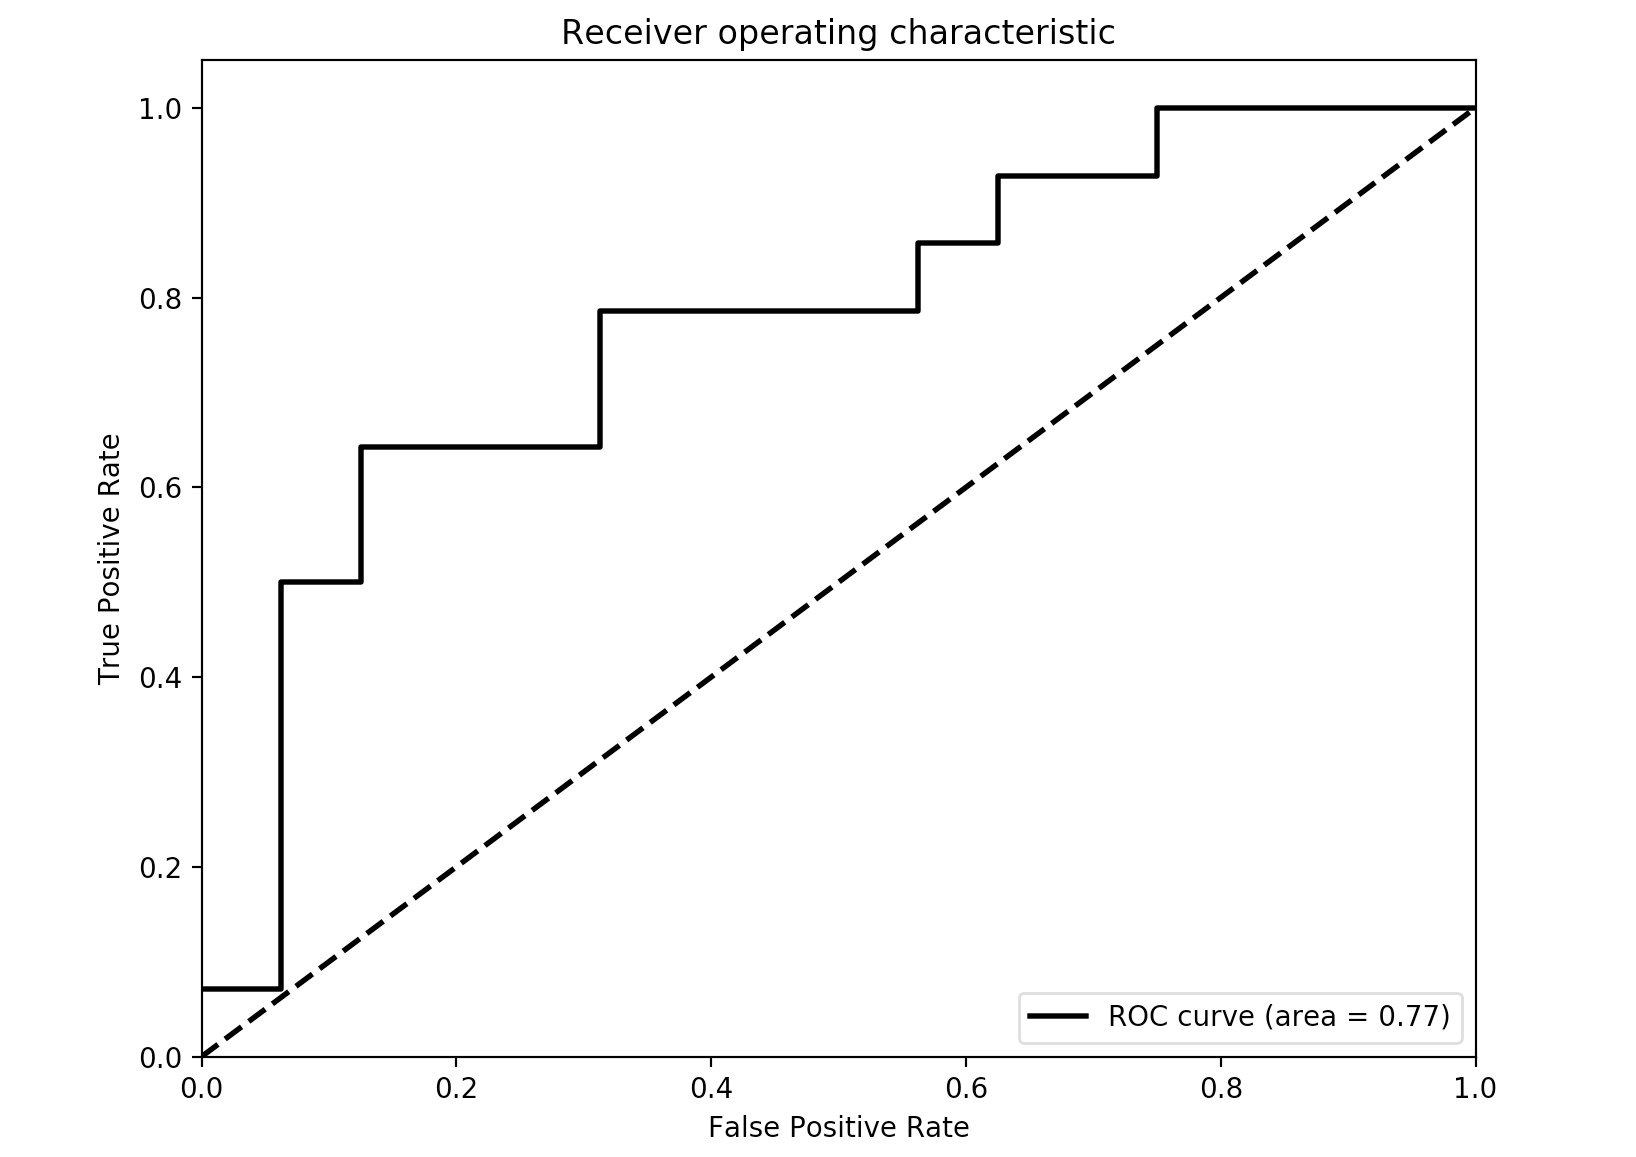
\includegraphics[width=\linewidth]{./imagenes/7_roc.png}
	\caption{Ejemplo curva ROC.}
	\label{img:roc}
\end{figure}

Para ver si un clasificador es bueno podemos calcular el área bajo la curva ROC. A mayor valor de área, mejor es el clasificador. En la imagen \ref{img:roc} podemos ver una línea discontinua. Dicha línea representa un área de \textit{0.5}. En dicha imagen también podemos ver que el área calculada es de \textit{0.77}, un valor bastante aceptable.

\subsection{Media geométrica.} \label{subsec:gm}

La media geométrica \cite{gm} se define como:

\begin{equation}
	g = \sqrt{a^+ \cdot a^-}
\end{equation}

donde a$^+$ denota la precisión en las instancias positivas —esto es \textit{TPR}— y a$^-$ denota la precisión en las instancias positivas —esto es \textit{TNR}—. \textit{TPR} calcula como hemos visto en la ecuación \ref{eq:tpr} y \textit{TNR} se calcula de la siguiente forma:

\begin{equation}
	TNR = \frac{TP}{TP + FN}
\end{equation}

Esta métrica une dos objetivos; busca maximizar la precisión a la vez que equilibrar el tamaño de ambas clases.

\section{Resultados numéricos.} \label{sec:resultados_numericos}

A continuación se muestran varias tablas donde iremos analizando los resultados obtenidos por los distintos algoritmos. Como se ha comentado en la sección \ref{sec:clasificacion} se ha usado \textit{k-fold} y la cantidad de datos recogida es abrumadora. Es por ello que, a continuación, se muestran las tablas con los valores medios de las cinco ejecuciones. Dichas tablas tienen un formato bastante colorido, ya que se ha aplicado un coloreado basado en \textit{mapas de calor}. Esta técnica colorea las celdas con un color más cálido —en este caso colores rojizos— cuanto mejor es el valor representado por dicha celda y un color más frío —en este caso colores azules— cuanto peor es el valor representado por dicha celda. En las tablas \ref{tab:tamanio_reducido}, \ref{tab:porcentaje_reducido} y \ref{tab:ir} se ha aplicado por filas, pudiendo comparar así el comportamiento de cada algoritmo. En las tablas \ref{tab:metricas_pt1}, \ref{tab:metricas_pt2}, \ref{tab:metricas_pt3} y \ref{tab:metricas_pt4} se ha aplicado por columnas, permitiendo comparar los algoritmos y ver el mejor valor de cada métrica. En el apéndice \ref{ch:apendice} se encuentran las tablas con toda la información recogida, para que se pueda verificar que las tablas presentadas en esta sección son reales. \\

Todas las ejecuciones han sido realizadas con los valores por defecto de los parámetros. Dichos valores los podemos ver en la sección \ref{sec:implementacion_algoritmos} o en la página web que contiene la documentación del proyecto, \href{https://nestorrv.github.io}{https://nestorrv.github.io}. \\

Para comparar como de efectivo es el proceso de reducción se ha comparado el tamaño del conjunto de datos antes y después de la aplicación de los algoritmos. Esta comparación la podemos ver en la tabla \ref{tab:tamanio_reducido}. Por lo general, el algoritmo que mejor se comporta es \textit{IPADE-ID} \cite{ipade}, junto con \textit{CPM} \cite{cpm}. En la tabla \ref{tab:porcentaje_reducido} podemos ver los porcentajes de reducción para los distintos algoritmos. Si nos fijamos en los valores medios, podemos ver que se obtiene un alto porcentaje de reducción, en torno a la mitad del tamaño original. \\

En la tabla \ref{tab:ir} podemos ver como se comporta el \textit{Imbalanced Ratio} tras aplicar los distintos algoritmos. En este caso, el algoritmo que mejor se comporta —por lo general— es \textit{IHTS} \cite{ihts} junto con \textit{ClusterOSS} \cite{clusteross}. Si nos fijamos en los valores medios, podemos ver que se obtiene un \textit{Imbalanced Ratio} bastante menor que en el conjunto de datos original, lo cual nos indica que se ha conseguido una mejor proporción de instancias positivas con respecto a instancias negativas. \\

En las tablas \ref{tab:metricas_pt1}, \ref{tab:metricas_pt2}, \ref{tab:metricas_pt3} y \ref{tab:metricas_pt4} podemos ver los valores medios de las métricas comentadas en la sección \ref{sec:clasificacion} para las cinco ejecuciones —obtenidas al aplicar \textit{k-fold}— de los conjuntos de datos antes y después de ser reducidos por los algoritmos. Como podemos ver, los valores medios obtenidos tras aplicar los algoritmos es bastante similar a la media de los conjuntos de datos original —los cuales podemos ver en la fila identificada por \textit{original}—. En todos los casos, hay un algoritmo que mejora los valores del conjunto original. \\

Tal y como hemos visto en esta sección, realizar un proceso de \textit{undersampling} aporta ventajas, pero tiene un inconveniente, y es que no es un proceso gratis. Este proceso lleva asociado un tiempo de ejecución. En la tabla \ref{tab:tiempos} podemos ver los tiempos de ejecución de cada algoritmo en cada conjunto de datos. El formato de dicha tabla es: \textit{minutos:segundos:milisegundos}. Como podemos ver, la mayoría de los algoritmos son bastante rápidos, excepto \textit{EUS} \cite{eus} e \textit{IPADE-ID}, ya que al ser algoritmos evolutivos necesitan más tiempo de ejecución. 

\hvFloat[
 floatPos=!htb,
 capWidth=h,
 capPos=r,
 capAngle=90,
 objectAngle=90,
 capVPos=c,
 objectPos=c]{table}{\scalebox{0.7}{\begin{tabular}{l|c|ccccccccccccccc|c}
\textbf{Dataset} & \textbf{Tamaño Original} & \textbf{BC} & \textbf{ClusterOSS} & \textbf{CNN} & \textbf{CPM} & \textbf{EE} & \textbf{ENN} & \textbf{EUS} & \textbf{IHTS} & \textbf{IPADE} & \textbf{NCL} & \textbf{NM} & \textbf{OSS} & \textbf{RU} & \textbf{SBC} & \textbf{TL} & \textbf{Media} \\
\midrule
\textbf{ecoli-0\_vs\_1} & 220   & \cellcolor[rgb]{ .988,  .988,  1}154 & \cellcolor[rgb]{ .976,  .608,  .616}64 & \cellcolor[rgb]{ .973,  .412,  .42}17 & \cellcolor[rgb]{ .973,  .416,  .424}18 & \cellcolor[rgb]{ .988,  .988,  1}154 & \cellcolor[rgb]{ .353,  .541,  .776}220 & \cellcolor[rgb]{ .988,  .988,  1}154 & \cellcolor[rgb]{ .98,  .784,  .796}106 & \cellcolor[rgb]{ .973,  .42,  .427}19 & \cellcolor[rgb]{ .451,  .612,  .812}210 & \cellcolor[rgb]{ .988,  .988,  1}154 & \cellcolor[rgb]{ .984,  .875,  .882}127 & \cellcolor[rgb]{ .988,  .988,  1}154 & \cellcolor[rgb]{ .443,  .604,  .808}211 & \cellcolor[rgb]{ .451,  .612,  .812}210 & 131.46667 \\
\textbf{ecoli1} & 336   & \cellcolor[rgb]{ .988,  .988,  1}154 & \cellcolor[rgb]{ .973,  .502,  .514}56 & \cellcolor[rgb]{ .976,  .624,  .631}80 & \cellcolor[rgb]{ .976,  .647,  .655}85 & \cellcolor[rgb]{ .988,  .988,  1}154 & \cellcolor[rgb]{ .353,  .541,  .776}321 & \cellcolor[rgb]{ .988,  .988,  1}154 & \cellcolor[rgb]{ .976,  .663,  .671}88 & \cellcolor[rgb]{ .973,  .412,  .42}37 & \cellcolor[rgb]{ .439,  .604,  .808}299 & \cellcolor[rgb]{ .988,  .988,  1}154 & \cellcolor[rgb]{ .718,  .796,  .906}226 & \cellcolor[rgb]{ .988,  .988,  1}154 & \cellcolor[rgb]{ .471,  .624,  .82}291 & \cellcolor[rgb]{ .451,  .612,  .812}296 & 169.93333 \\
\textbf{ecoli2} & 336   & \cellcolor[rgb]{ .988,  .988,  1}104 & \cellcolor[rgb]{ .973,  .482,  .49}34 & \cellcolor[rgb]{ .98,  .722,  .729}67 & \cellcolor[rgb]{ .976,  .69,  .702}63 & \cellcolor[rgb]{ .988,  .988,  1}104 & \cellcolor[rgb]{ .353,  .541,  .776}329 & \cellcolor[rgb]{ .988,  .988,  1}104 & \cellcolor[rgb]{ .976,  .69,  .702}63 & \cellcolor[rgb]{ .973,  .412,  .42}24 & \cellcolor[rgb]{ .388,  .569,  .792}317 & \cellcolor[rgb]{ .988,  .988,  1}104 & \cellcolor[rgb]{ .49,  .639,  .827}281 & \cellcolor[rgb]{ .988,  .988,  1}104 & \cellcolor[rgb]{ .412,  .584,  .8}309 & \cellcolor[rgb]{ .404,  .576,  .796}312 & 154.6 \\
\textbf{ecoli3} & 336   & \cellcolor[rgb]{ .988,  .988,  1}70 & \cellcolor[rgb]{ .973,  .549,  .561}42 & \cellcolor[rgb]{ .984,  .894,  .906}64 & \cellcolor[rgb]{ .976,  .675,  .686}50 & \cellcolor[rgb]{ .988,  .988,  1}70 & \cellcolor[rgb]{ .353,  .541,  .776}324 & \cellcolor[rgb]{ .988,  .988,  1}70 & \cellcolor[rgb]{ .976,  .627,  .639}47 & \cellcolor[rgb]{ .973,  .412,  .42}33 & \cellcolor[rgb]{ .38,  .561,  .788}314 & \cellcolor[rgb]{ .988,  .988,  1}70 & \cellcolor[rgb]{ .541,  .675,  .843}250 & \cellcolor[rgb]{ .988,  .988,  1}70 & \cellcolor[rgb]{ .408,  .58,  .796}303 & \cellcolor[rgb]{ .388,  .569,  .792}310 & 139.13333 \\
\textbf{glass-0-1-2-3\_vs\_4-5-6} & 214   & \cellcolor[rgb]{ .988,  .988,  1}102 & \cellcolor[rgb]{ .973,  .424,  .435}30 & \cellcolor[rgb]{ .973,  .431,  .443}31 & \cellcolor[rgb]{ .973,  .412,  .42}28 & \cellcolor[rgb]{ .988,  .988,  1}102 & \cellcolor[rgb]{ .353,  .541,  .776}206 & \cellcolor[rgb]{ .988,  .988,  1}102 & \cellcolor[rgb]{ .976,  .627,  .639}56 & \cellcolor[rgb]{ .973,  .431,  .443}31 & \cellcolor[rgb]{ .416,  .584,  .8}196 & \cellcolor[rgb]{ .988,  .988,  1}102 & \cellcolor[rgb]{ .416,  .584,  .8}196 & \cellcolor[rgb]{ .988,  .988,  1}102 & \cellcolor[rgb]{ .38,  .561,  .788}202 & \cellcolor[rgb]{ .38,  .561,  .788}202 & 112.53333 \\
\textbf{glass0} & 214   & \cellcolor[rgb]{ .988,  .988,  1}140 & \cellcolor[rgb]{ .973,  .427,  .435}41 & \cellcolor[rgb]{ .976,  .635,  .647}78 & \cellcolor[rgb]{ .976,  .604,  .612}72 & \cellcolor[rgb]{ .988,  .988,  1}140 & \cellcolor[rgb]{ .353,  .541,  .776}183 & \cellcolor[rgb]{ .988,  .988,  1}140 & \cellcolor[rgb]{ .98,  .749,  .761}98 & \cellcolor[rgb]{ .973,  .412,  .42}38 & \cellcolor[rgb]{ .533,  .667,  .839}171 & \cellcolor[rgb]{ .988,  .988,  1}140 & \cellcolor[rgb]{ .984,  .953,  .965}134 & \cellcolor[rgb]{ .988,  .988,  1}140 & \cellcolor[rgb]{ .443,  .604,  .808}177 & \cellcolor[rgb]{ .545,  .678,  .847}170 & 124.13333 \\
\textbf{glass1} & 214   & \cellcolor[rgb]{ .988,  .988,  1}152 & \cellcolor[rgb]{ .973,  .412,  .42}34 & \cellcolor[rgb]{ .976,  .671,  .678}87 & \cellcolor[rgb]{ .976,  .639,  .647}81 & \cellcolor[rgb]{ .988,  .988,  1}152 & \cellcolor[rgb]{ .353,  .541,  .776}192 & \cellcolor[rgb]{ .988,  .988,  1}152 & \cellcolor[rgb]{ .98,  .804,  .816}115 & \cellcolor[rgb]{ .973,  .439,  .447}40 & \cellcolor[rgb]{ .69,  .776,  .894}171 & \cellcolor[rgb]{ .988,  .988,  1}152 & \cellcolor[rgb]{ .816,  .867,  .941}163 & \cellcolor[rgb]{ .988,  .988,  1}152 & \cellcolor[rgb]{ .467,  .62,  .816}185 & \cellcolor[rgb]{ .671,  .765,  .89}172 & 133.33333 \\
\textbf{glass6} & 214   & \cellcolor[rgb]{ .988,  .988,  1}58 & \cellcolor[rgb]{ .976,  .663,  .671}36 & \cellcolor[rgb]{ .973,  .412,  .42}19 & \cellcolor[rgb]{ .973,  .455,  .463}22 & \cellcolor[rgb]{ .988,  .988,  1}58 & \cellcolor[rgb]{ .353,  .541,  .776}213 & \cellcolor[rgb]{ .988,  .988,  1}58 & \cellcolor[rgb]{ .976,  .631,  .639}34 & \cellcolor[rgb]{ .973,  .514,  .522}26 & \cellcolor[rgb]{ .416,  .588,  .8}198 & \cellcolor[rgb]{ .988,  .988,  1}58 & \cellcolor[rgb]{ .871,  .906,  .961}87 & \cellcolor[rgb]{ .988,  .988,  1}58 & \cellcolor[rgb]{ .4,  .576,  .796}202 & \cellcolor[rgb]{ .4,  .576,  .796}202 & 88.6 \\
\textbf{haberman} & 306   & \cellcolor[rgb]{ .988,  .988,  1}162 & \cellcolor[rgb]{ .973,  .49,  .498}55 & \cellcolor[rgb]{ .984,  .984,  1}163 & \cellcolor[rgb]{ .984,  .918,  .929}147 & \cellcolor[rgb]{ .988,  .988,  1}162 & \cellcolor[rgb]{ .353,  .541,  .776}273 & \cellcolor[rgb]{ .984,  .984,  1}163 & \cellcolor[rgb]{ .976,  .616,  .624}82 & \cellcolor[rgb]{ .973,  .412,  .42}38 & \cellcolor[rgb]{ .573,  .698,  .855}235 & \cellcolor[rgb]{ .988,  .988,  1}162 & \cellcolor[rgb]{ .769,  .831,  .922}201 & \cellcolor[rgb]{ .988,  .988,  1}162 & \cellcolor[rgb]{ .722,  .8,  .906}209 & \cellcolor[rgb]{ .706,  .788,  .902}212 & 161.73333 \\
\textbf{iris0} & 150   & \cellcolor[rgb]{ .988,  .988,  1}100 & \cellcolor[rgb]{ .973,  .475,  .482}13 & \cellcolor[rgb]{ .973,  .412,  .42}2 & \cellcolor[rgb]{ .973,  .412,  .42}2 & \cellcolor[rgb]{ .988,  .988,  1}100 & \cellcolor[rgb]{ .353,  .541,  .776}150 & \cellcolor[rgb]{ .988,  .988,  1}100 & \cellcolor[rgb]{ .98,  .8,  .808}68 & \cellcolor[rgb]{ .973,  .475,  .482}13 & \cellcolor[rgb]{ .353,  .541,  .776}150 & \cellcolor[rgb]{ .988,  .988,  1}100 & \cellcolor[rgb]{ .976,  .686,  .694}49 & \cellcolor[rgb]{ .988,  .988,  1}100 & \cellcolor[rgb]{ .38,  .561,  .788}148 & \cellcolor[rgb]{ .404,  .58,  .796}146 & 82.73333 \\
\textbf{new-thyroid1} & 215   & \cellcolor[rgb]{ .988,  .988,  1}70 & \cellcolor[rgb]{ .98,  .702,  .714}41 & \cellcolor[rgb]{ .973,  .412,  .42}11 & \cellcolor[rgb]{ .973,  .427,  .439}13 & \cellcolor[rgb]{ .988,  .988,  1}70 & \cellcolor[rgb]{ .353,  .541,  .776}213 & \cellcolor[rgb]{ .988,  .988,  1}70 & \cellcolor[rgb]{ .984,  .969,  .976}68 & \cellcolor[rgb]{ .973,  .537,  .545}24 & \cellcolor[rgb]{ .404,  .576,  .796}202 & \cellcolor[rgb]{ .988,  .988,  1}70 & \cellcolor[rgb]{ .984,  .898,  .91}61 & \cellcolor[rgb]{ .988,  .988,  1}70 & \cellcolor[rgb]{ .376,  .557,  .784}208 & \cellcolor[rgb]{ .392,  .569,  .792}205 & 93.06667 \\
\textbf{new-thyroid2} & 215   & \cellcolor[rgb]{ .988,  .988,  1}70 & \cellcolor[rgb]{ .976,  .631,  .639}36 & \cellcolor[rgb]{ .973,  .412,  .42}15 & \cellcolor[rgb]{ .973,  .42,  .427}16 & \cellcolor[rgb]{ .988,  .988,  1}70 & \cellcolor[rgb]{ .353,  .541,  .776}213 & \cellcolor[rgb]{ .988,  .988,  1}70 & \cellcolor[rgb]{ .976,  .671,  .682}40 & \cellcolor[rgb]{ .973,  .494,  .502}23 & \cellcolor[rgb]{ .4,  .573,  .792}203 & \cellcolor[rgb]{ .988,  .988,  1}70 & \cellcolor[rgb]{ .886,  .918,  .965}93 & \cellcolor[rgb]{ .988,  .988,  1}70 & \cellcolor[rgb]{ .384,  .565,  .788}206 & \cellcolor[rgb]{ .392,  .569,  .792}205 & 93.33333 \\
\textbf{page-blocks0} & 5472  & \cellcolor[rgb]{ .988,  .988,  1}1118 & \cellcolor[rgb]{ .976,  .624,  .635}502 & \cellcolor[rgb]{ .976,  .631,  .643}514 & \cellcolor[rgb]{ .976,  .631,  .643}514 & \cellcolor[rgb]{ .988,  .988,  1}1118 & \cellcolor[rgb]{ .353,  .541,  .776}5410 & \cellcolor[rgb]{ .984,  .984,  .996}1117 & \cellcolor[rgb]{ .98,  .722,  .729}665 & \cellcolor[rgb]{ .973,  .412,  .42}135 & \cellcolor[rgb]{ .376,  .561,  .788}5255 & \cellcolor[rgb]{ .988,  .988,  1}1118 & \cellcolor[rgb]{ .475,  .627,  .82}4598 & \cellcolor[rgb]{ .988,  .988,  1}1118 & \cellcolor[rgb]{ .667,  .761,  .886}3312 & \cellcolor[rgb]{ .388,  .565,  .788}5186 & 2112 \\
\textbf{pima} & 768   & \cellcolor[rgb]{ .988,  .988,  1}536 & \cellcolor[rgb]{ .973,  .537,  .545}161 & \cellcolor[rgb]{ .98,  .796,  .808}377 & \cellcolor[rgb]{ .98,  .792,  .804}374 & \cellcolor[rgb]{ .988,  .988,  1}536 & \cellcolor[rgb]{ .353,  .541,  .776}678 & \cellcolor[rgb]{ .984,  .984,  .996}535 & \cellcolor[rgb]{ .976,  .686,  .698}287 & \cellcolor[rgb]{ .973,  .412,  .42}55 & \cellcolor[rgb]{ .792,  .851,  .933}580 & \cellcolor[rgb]{ .988,  .988,  1}536 & \cellcolor[rgb]{ .98,  .984,  1}538 & \cellcolor[rgb]{ .988,  .988,  1}536 & \cellcolor[rgb]{ .988,  .988,  1}536 & \cellcolor[rgb]{ .89,  .922,  .969}558 & 454.86667 \\
\textbf{segment0} & 2308  & \cellcolor[rgb]{ .988,  .988,  1}658 & \cellcolor[rgb]{ .976,  .643,  .651}287 & \cellcolor[rgb]{ .973,  .439,  .447}69 & \cellcolor[rgb]{ .973,  .435,  .443}65 & \cellcolor[rgb]{ .988,  .988,  1}658 & \cellcolor[rgb]{ .353,  .541,  .776}2290 & \cellcolor[rgb]{ .984,  .98,  .992}652 & \cellcolor[rgb]{ .965,  .973,  .992}725 & \cellcolor[rgb]{ .973,  .412,  .42}38 & \cellcolor[rgb]{ .361,  .545,  .78}2277 & \cellcolor[rgb]{ .988,  .988,  1}658 & \cellcolor[rgb]{ .529,  .667,  .839}1841 & \cellcolor[rgb]{ .988,  .988,  1}658 & \cellcolor[rgb]{ .533,  .671,  .843}1830 & \cellcolor[rgb]{ .4,  .576,  .796}2172 & 991.86667 \\
\textbf{vehicle0} & 846   & \cellcolor[rgb]{ .988,  .988,  1}398 & \cellcolor[rgb]{ .973,  .541,  .553}148 & \cellcolor[rgb]{ .973,  .518,  .525}133 & \cellcolor[rgb]{ .973,  .553,  .561}154 & \cellcolor[rgb]{ .988,  .988,  1}398 & \cellcolor[rgb]{ .353,  .541,  .776}829 & \cellcolor[rgb]{ .988,  .988,  1}399 & \cellcolor[rgb]{ .984,  .894,  .902}345 & \cellcolor[rgb]{ .973,  .412,  .42}73 & \cellcolor[rgb]{ .416,  .588,  .8}787 & \cellcolor[rgb]{ .988,  .988,  1}398 & \cellcolor[rgb]{ .51,  .651,  .831}724 & \cellcolor[rgb]{ .988,  .988,  1}398 & \cellcolor[rgb]{ .561,  .686,  .851}690 & \cellcolor[rgb]{ .494,  .643,  .827}734 & 440.53333 \\
\textbf{vehicle1} & 846   & \cellcolor[rgb]{ .988,  .988,  1}434 & \cellcolor[rgb]{ .973,  .467,  .475}187 & \cellcolor[rgb]{ .984,  .871,  .882}380 & \cellcolor[rgb]{ .984,  .886,  .894}386 & \cellcolor[rgb]{ .988,  .988,  1}434 & \cellcolor[rgb]{ .353,  .541,  .776}756 & \cellcolor[rgb]{ .984,  .961,  .973}422 & \cellcolor[rgb]{ .976,  .69,  .698}293 & \cellcolor[rgb]{ .973,  .412,  .42}161 & \cellcolor[rgb]{ .541,  .675,  .843}661 & \cellcolor[rgb]{ .988,  .988,  1}434 & \cellcolor[rgb]{ .639,  .741,  .878}612 & \cellcolor[rgb]{ .988,  .988,  1}434 & \cellcolor[rgb]{ .733,  .808,  .91}565 & \cellcolor[rgb]{ .627,  .733,  .875}618 & 451.8 \\
\textbf{vehicle2} & 846   & \cellcolor[rgb]{ .988,  .988,  1}436 & \cellcolor[rgb]{ .976,  .573,  .58}161 & \cellcolor[rgb]{ .973,  .537,  .545}138 & \cellcolor[rgb]{ .973,  .545,  .553}143 & \cellcolor[rgb]{ .988,  .988,  1}436 & \cellcolor[rgb]{ .353,  .541,  .776}816 & \cellcolor[rgb]{ .984,  .98,  .992}433 & \cellcolor[rgb]{ .984,  .863,  .871}353 & \cellcolor[rgb]{ .973,  .412,  .42}53 & \cellcolor[rgb]{ .412,  .58,  .796}783 & \cellcolor[rgb]{ .988,  .988,  1}436 & \cellcolor[rgb]{ .502,  .647,  .831}729 & \cellcolor[rgb]{ .988,  .988,  1}436 & \cellcolor[rgb]{ .69,  .78,  .898}616 & \cellcolor[rgb]{ .49,  .635,  .824}736 & 447 \\
\textbf{vehicle3} & 846   & \cellcolor[rgb]{ .988,  .988,  1}424 & \cellcolor[rgb]{ .973,  .412,  .42}127 & \cellcolor[rgb]{ .984,  .855,  .867}356 & \cellcolor[rgb]{ .984,  .882,  .894}370 & \cellcolor[rgb]{ .988,  .988,  1}424 & \cellcolor[rgb]{ .353,  .541,  .776}774 & \cellcolor[rgb]{ .984,  .973,  .984}417 & \cellcolor[rgb]{ .929,  .945,  .98}458 & \cellcolor[rgb]{ .973,  .416,  .424}131 & \cellcolor[rgb]{ .537,  .671,  .843}674 & \cellcolor[rgb]{ .988,  .988,  1}424 & \cellcolor[rgb]{ .651,  .753,  .882}610 & \cellcolor[rgb]{ .988,  .988,  1}424 & \cellcolor[rgb]{ .745,  .82,  .918}558 & \cellcolor[rgb]{ .627,  .733,  .875}624 & 453 \\
\textbf{wisconsin} & 683   & \cellcolor[rgb]{ .988,  .988,  1}478 & \cellcolor[rgb]{ .973,  .412,  .42}28 & \cellcolor[rgb]{ .973,  .471,  .478}74 & \cellcolor[rgb]{ .973,  .467,  .475}73 & \cellcolor[rgb]{ .988,  .988,  1}478 & \cellcolor[rgb]{ .384,  .565,  .788}672 & \cellcolor[rgb]{ .988,  .988,  1}478 & \cellcolor[rgb]{ .984,  .914,  .925}421 & \cellcolor[rgb]{ .973,  .439,  .447}52 & \cellcolor[rgb]{ .416,  .584,  .8}662 & \cellcolor[rgb]{ .988,  .988,  1}478 & \cellcolor[rgb]{ .98,  .761,  .773}303 & \cellcolor[rgb]{ .988,  .988,  1}478 & \cellcolor[rgb]{ .353,  .541,  .776}681 & \cellcolor[rgb]{ .412,  .584,  .8}663 & 401.26667 \\
\textbf{yeast1} & 1484  & \cellcolor[rgb]{ .988,  .988,  1}858 & \cellcolor[rgb]{ .973,  .525,  .537}294 & \cellcolor[rgb]{ .984,  .843,  .855}681 & \cellcolor[rgb]{ .984,  .855,  .867}696 & \cellcolor[rgb]{ .988,  .988,  1}858 & \cellcolor[rgb]{ .514,  .655,  .835}1325 & \cellcolor[rgb]{ .988,  .988,  1}859 & \cellcolor[rgb]{ .98,  .702,  .71}508 & \cellcolor[rgb]{ .973,  .412,  .42}150 & \cellcolor[rgb]{ .698,  .784,  .898}1146 & \cellcolor[rgb]{ .988,  .988,  1}858 & \cellcolor[rgb]{ .733,  .808,  .91}1111 & \cellcolor[rgb]{ .988,  .988,  1}858 & \cellcolor[rgb]{ .353,  .541,  .776}1481 & \cellcolor[rgb]{ .729,  .808,  .91}1114 & 853.13333 \\
\textbf{yeast3} & 1484  & \cellcolor[rgb]{ .988,  .988,  1}326 & \cellcolor[rgb]{ .976,  .557,  .565}151 & \cellcolor[rgb]{ .98,  .788,  .796}245 & \cellcolor[rgb]{ .98,  .769,  .78}238 & \cellcolor[rgb]{ .988,  .988,  1}326 & \cellcolor[rgb]{ .353,  .541,  .776}1451 & \cellcolor[rgb]{ .988,  .988,  1}326 & \cellcolor[rgb]{ .976,  .624,  .635}179 & \cellcolor[rgb]{ .973,  .412,  .42}92 & \cellcolor[rgb]{ .388,  .565,  .788}1395 & \cellcolor[rgb]{ .988,  .988,  1}326 & \cellcolor[rgb]{ .404,  .58,  .796}1362 & \cellcolor[rgb]{ .988,  .988,  1}326 & \cellcolor[rgb]{ .549,  .678,  .847}1109 & \cellcolor[rgb]{ .404,  .58,  .796}1362 & 614.26667 \\
\end{tabular}}}{Tamaño de los conjuntos de datos reducidos.}{tab:tamanio_reducido}

\hvFloat[
 floatPos=!htb,
 capWidth=h,
 capPos=r,
 capAngle=90,
 objectAngle=90,
 capVPos=c,
 objectPos=c]{table}{\scalebox{0.7}{\begin{tabular}{l|ccccccccccccccc|c}
\textbf{Dataset} & \textbf{BC} & \textbf{ClusterOSS} & \textbf{CNN} & \textbf{CPM} & \textbf{EE} & \textbf{ENN} & \textbf{EUS} & \textbf{IHTS} & \textbf{IPADE} & \textbf{NCL} & \textbf{NM} & \textbf{OSS} & \textbf{RU} & \textbf{SBC} & \textbf{TL} & \textbf{Media} \\
\midrule
\textbf{ecoli-0\_vs\_1} & \cellcolor[rgb]{ .988,  .988,  1}30 & \cellcolor[rgb]{ .98,  .612,  .62}70.91 & \cellcolor[rgb]{ .973,  .412,  .42}92.27 & \cellcolor[rgb]{ .976,  .42,  .427}91.82 & \cellcolor[rgb]{ .988,  .988,  1}30 & \cellcolor[rgb]{ .353,  .541,  .776}0 & \cellcolor[rgb]{ .988,  .988,  1}30 & \cellcolor[rgb]{ .984,  .788,  .8}51.82 & \cellcolor[rgb]{ .976,  .424,  .431}91.36 & \cellcolor[rgb]{ .447,  .608,  .808}4.55 & \cellcolor[rgb]{ .988,  .988,  1}30 & \cellcolor[rgb]{ .988,  .878,  .886}42.27 & \cellcolor[rgb]{ .988,  .988,  1}30 & \cellcolor[rgb]{ .439,  .6,  .804}4.09 & \cellcolor[rgb]{ .447,  .608,  .808}4.55 & 40.24 \\
\textbf{ecoli1} & \cellcolor[rgb]{ .988,  .988,  1}54.17 & \cellcolor[rgb]{ .976,  .506,  .518}83.33 & \cellcolor[rgb]{ .98,  .627,  .635}76.19 & \cellcolor[rgb]{ .98,  .651,  .659}74.7 & \cellcolor[rgb]{ .988,  .988,  1}54.17 & \cellcolor[rgb]{ .353,  .541,  .776}4.46 & \cellcolor[rgb]{ .988,  .988,  1}54.17 & \cellcolor[rgb]{ .98,  .667,  .675}73.81 & \cellcolor[rgb]{ .973,  .412,  .42}88.99 & \cellcolor[rgb]{ .435,  .6,  .804}11.01 & \cellcolor[rgb]{ .988,  .988,  1}54.17 & \cellcolor[rgb]{ .714,  .792,  .902}32.74 & \cellcolor[rgb]{ .988,  .988,  1}54.17 & \cellcolor[rgb]{ .467,  .62,  .816}13.39 & \cellcolor[rgb]{ .447,  .608,  .808}11.9 & 49.42 \\
\textbf{ecoli2} & \cellcolor[rgb]{ .988,  .988,  1}69.05 & \cellcolor[rgb]{ .976,  .486,  .494}89.88 & \cellcolor[rgb]{ .984,  .725,  .733}80.06 & \cellcolor[rgb]{ .98,  .694,  .706}81.25 & \cellcolor[rgb]{ .988,  .988,  1}69.05 & \cellcolor[rgb]{ .353,  .541,  .776}2.08 & \cellcolor[rgb]{ .988,  .988,  1}69.05 & \cellcolor[rgb]{ .98,  .694,  .706}81.25 & \cellcolor[rgb]{ .973,  .412,  .42}92.86 & \cellcolor[rgb]{ .384,  .565,  .788}5.65 & \cellcolor[rgb]{ .988,  .988,  1}69.05 & \cellcolor[rgb]{ .486,  .635,  .824}16.37 & \cellcolor[rgb]{ .988,  .988,  1}69.05 & \cellcolor[rgb]{ .408,  .58,  .796}8.04 & \cellcolor[rgb]{ .4,  .573,  .792}7.14 & 53.99 \\
\textbf{ecoli3} & \cellcolor[rgb]{ .988,  .988,  1}79.17 & \cellcolor[rgb]{ .976,  .553,  .565}87.5 & \cellcolor[rgb]{ .988,  .898,  .91}80.95 & \cellcolor[rgb]{ .98,  .678,  .69}85.12 & \cellcolor[rgb]{ .988,  .988,  1}79.17 & \cellcolor[rgb]{ .353,  .541,  .776}3.57 & \cellcolor[rgb]{ .988,  .988,  1}79.17 & \cellcolor[rgb]{ .98,  .631,  .643}86.01 & \cellcolor[rgb]{ .973,  .412,  .42}90.18 & \cellcolor[rgb]{ .376,  .557,  .784}6.55 & \cellcolor[rgb]{ .988,  .988,  1}79.17 & \cellcolor[rgb]{ .537,  .671,  .839}25.6 & \cellcolor[rgb]{ .988,  .988,  1}79.17 & \cellcolor[rgb]{ .404,  .576,  .792}9.82 & \cellcolor[rgb]{ .384,  .565,  .788}7.74 & 58.59 \\
\textbf{glass-0-1-2-3\_vs\_4-5-6} & \cellcolor[rgb]{ .988,  .988,  1}52.34 & \cellcolor[rgb]{ .976,  .427,  .439}85.98 & \cellcolor[rgb]{ .976,  .435,  .447}85.51 & \cellcolor[rgb]{ .973,  .412,  .42}86.92 & \cellcolor[rgb]{ .988,  .988,  1}52.34 & \cellcolor[rgb]{ .353,  .541,  .776}3.74 & \cellcolor[rgb]{ .988,  .988,  1}52.34 & \cellcolor[rgb]{ .98,  .631,  .643}73.83 & \cellcolor[rgb]{ .976,  .435,  .447}85.51 & \cellcolor[rgb]{ .412,  .58,  .796}8.41 & \cellcolor[rgb]{ .988,  .988,  1}52.34 & \cellcolor[rgb]{ .412,  .58,  .796}8.41 & \cellcolor[rgb]{ .988,  .988,  1}52.34 & \cellcolor[rgb]{ .376,  .557,  .784}5.61 & \cellcolor[rgb]{ .376,  .557,  .784}5.61 & 47.41 \\
\textbf{glass0} & \cellcolor[rgb]{ .988,  .988,  1}34.58 & \cellcolor[rgb]{ .976,  .431,  .439}80.84 & \cellcolor[rgb]{ .98,  .639,  .651}63.55 & \cellcolor[rgb]{ .98,  .604,  .616}66.36 & \cellcolor[rgb]{ .988,  .988,  1}34.58 & \cellcolor[rgb]{ .353,  .541,  .776}14.49 & \cellcolor[rgb]{ .988,  .988,  1}34.58 & \cellcolor[rgb]{ .984,  .753,  .765}54.21 & \cellcolor[rgb]{ .973,  .412,  .42}82.24 & \cellcolor[rgb]{ .529,  .663,  .835}20.09 & \cellcolor[rgb]{ .988,  .988,  1}34.58 & \cellcolor[rgb]{ .988,  .957,  .969}37.38 & \cellcolor[rgb]{ .988,  .988,  1}34.58 & \cellcolor[rgb]{ .439,  .6,  .804}17.29 & \cellcolor[rgb]{ .541,  .675,  .843}20.56 & 41.99 \\
\textbf{glass1} & \cellcolor[rgb]{ .988,  .988,  1}28.97 & \cellcolor[rgb]{ .973,  .412,  .42}84.11 & \cellcolor[rgb]{ .98,  .675,  .682}59.35 & \cellcolor[rgb]{ .98,  .643,  .651}62.15 & \cellcolor[rgb]{ .988,  .988,  1}28.97 & \cellcolor[rgb]{ .353,  .541,  .776}10.28 & \cellcolor[rgb]{ .988,  .988,  1}28.97 & \cellcolor[rgb]{ .984,  .808,  .82}46.26 & \cellcolor[rgb]{ .976,  .443,  .451}81.31 & \cellcolor[rgb]{ .686,  .773,  .89}20.09 & \cellcolor[rgb]{ .988,  .988,  1}28.97 & \cellcolor[rgb]{ .812,  .863,  .937}23.83 & \cellcolor[rgb]{ .988,  .988,  1}28.97 & \cellcolor[rgb]{ .463,  .616,  .812}13.55 & \cellcolor[rgb]{ .671,  .765,  .886}19.63 & 37.69 \\
\textbf{glass6} & \cellcolor[rgb]{ .988,  .988,  1}72.9 & \cellcolor[rgb]{ .98,  .667,  .675}83.18 & \cellcolor[rgb]{ .973,  .412,  .42}91.12 & \cellcolor[rgb]{ .976,  .459,  .467}89.72 & \cellcolor[rgb]{ .988,  .988,  1}72.9 & \cellcolor[rgb]{ .353,  .541,  .776}0.47 & \cellcolor[rgb]{ .988,  .988,  1}72.9 & \cellcolor[rgb]{ .98,  .635,  .643}84.11 & \cellcolor[rgb]{ .976,  .518,  .525}87.85 & \cellcolor[rgb]{ .412,  .584,  .796}7.48 & \cellcolor[rgb]{ .988,  .988,  1}72.9 & \cellcolor[rgb]{ .867,  .902,  .957}59.35 & \cellcolor[rgb]{ .988,  .988,  1}72.9 & \cellcolor[rgb]{ .396,  .573,  .792}5.61 & \cellcolor[rgb]{ .396,  .573,  .792}5.61 & 58.6 \\
\textbf{haberman} & \cellcolor[rgb]{ .988,  .988,  1}47.06 & \cellcolor[rgb]{ .976,  .494,  .502}82.03 & \cellcolor[rgb]{ .98,  .98,  .996}46.73 & \cellcolor[rgb]{ .988,  .922,  .933}51.96 & \cellcolor[rgb]{ .988,  .988,  1}47.06 & \cellcolor[rgb]{ .353,  .541,  .776}10.78 & \cellcolor[rgb]{ .98,  .98,  .996}46.73 & \cellcolor[rgb]{ .98,  .62,  .627}73.2 & \cellcolor[rgb]{ .973,  .412,  .42}87.58 & \cellcolor[rgb]{ .569,  .694,  .851}23.2 & \cellcolor[rgb]{ .988,  .988,  1}47.06 & \cellcolor[rgb]{ .765,  .827,  .918}34.31 & \cellcolor[rgb]{ .988,  .988,  1}47.06 & \cellcolor[rgb]{ .718,  .796,  .902}31.7 & \cellcolor[rgb]{ .702,  .784,  .898}30.72 & 47.15 \\
\textbf{iris0} & \cellcolor[rgb]{ .988,  .988,  1}33.33 & \cellcolor[rgb]{ .976,  .478,  .486}91.33 & \cellcolor[rgb]{ .973,  .412,  .42}98.67 & \cellcolor[rgb]{ .973,  .412,  .42}98.67 & \cellcolor[rgb]{ .988,  .988,  1}33.33 & \cellcolor[rgb]{ .353,  .541,  .776}0 & \cellcolor[rgb]{ .988,  .988,  1}33.33 & \cellcolor[rgb]{ .984,  .8,  .812}54.67 & \cellcolor[rgb]{ .976,  .478,  .486}91.33 & \cellcolor[rgb]{ .353,  .541,  .776}0 & \cellcolor[rgb]{ .988,  .988,  1}33.33 & \cellcolor[rgb]{ .98,  .69,  .698}67.33 & \cellcolor[rgb]{ .988,  .988,  1}33.33 & \cellcolor[rgb]{ .376,  .557,  .784}1.33 & \cellcolor[rgb]{ .4,  .576,  .792}2.67 & 44.84 \\
\textbf{new-thyroid1} & \cellcolor[rgb]{ .988,  .988,  1}67.44 & \cellcolor[rgb]{ .984,  .706,  .718}80.93 & \cellcolor[rgb]{ .973,  .412,  .42}94.88 & \cellcolor[rgb]{ .976,  .431,  .443}93.95 & \cellcolor[rgb]{ .988,  .988,  1}67.44 & \cellcolor[rgb]{ .353,  .541,  .776}0.93 & \cellcolor[rgb]{ .988,  .988,  1}67.44 & \cellcolor[rgb]{ .988,  .973,  .98}68.37 & \cellcolor[rgb]{ .976,  .541,  .549}88.84 & \cellcolor[rgb]{ .4,  .573,  .792}6.05 & \cellcolor[rgb]{ .988,  .988,  1}67.44 & \cellcolor[rgb]{ .988,  .902,  .914}71.63 & \cellcolor[rgb]{ .988,  .988,  1}67.44 & \cellcolor[rgb]{ .373,  .553,  .78}3.26 & \cellcolor[rgb]{ .388,  .565,  .788}4.65 & 56.71 \\
\textbf{new-thyroid2} & \cellcolor[rgb]{ .988,  .988,  1}67.44 & \cellcolor[rgb]{ .98,  .635,  .643}83.26 & \cellcolor[rgb]{ .973,  .412,  .42}93.02 & \cellcolor[rgb]{ .976,  .424,  .431}92.56 & \cellcolor[rgb]{ .988,  .988,  1}67.44 & \cellcolor[rgb]{ .353,  .541,  .776}0.93 & \cellcolor[rgb]{ .988,  .988,  1}67.44 & \cellcolor[rgb]{ .98,  .675,  .686}81.4 & \cellcolor[rgb]{ .976,  .498,  .506}89.3 & \cellcolor[rgb]{ .396,  .569,  .788}5.58 & \cellcolor[rgb]{ .988,  .988,  1}67.44 & \cellcolor[rgb]{ .882,  .914,  .961}56.74 & \cellcolor[rgb]{ .988,  .988,  1}67.44 & \cellcolor[rgb]{ .38,  .561,  .784}4.19 & \cellcolor[rgb]{ .388,  .565,  .788}4.65 & 56.59 \\
\textbf{page-blocks0} & \cellcolor[rgb]{ .988,  .988,  1}79.57 & \cellcolor[rgb]{ .98,  .627,  .639}90.83 & \cellcolor[rgb]{ .98,  .635,  .647}90.61 & \cellcolor[rgb]{ .98,  .635,  .647}90.61 & \cellcolor[rgb]{ .988,  .988,  1}79.57 & \cellcolor[rgb]{ .353,  .541,  .776}1.13 & \cellcolor[rgb]{ .988,  .988,  1}79.59 & \cellcolor[rgb]{ .984,  .725,  .733}87.85 & \cellcolor[rgb]{ .973,  .412,  .42}97.53 & \cellcolor[rgb]{ .373,  .557,  .784}3.97 & \cellcolor[rgb]{ .988,  .988,  1}79.57 & \cellcolor[rgb]{ .471,  .624,  .816}15.97 & \cellcolor[rgb]{ .988,  .988,  1}79.57 & \cellcolor[rgb]{ .663,  .757,  .882}39.47 & \cellcolor[rgb]{ .384,  .561,  .784}5.23 & 61.4 \\
\textbf{pima} & \cellcolor[rgb]{ .988,  .988,  1}30.21 & \cellcolor[rgb]{ .976,  .541,  .549}79.04 & \cellcolor[rgb]{ .984,  .8,  .812}50.91 & \cellcolor[rgb]{ .984,  .796,  .808}51.3 & \cellcolor[rgb]{ .988,  .988,  1}30.21 & \cellcolor[rgb]{ .353,  .541,  .776}11.72 & \cellcolor[rgb]{ .988,  .988,  1}30.34 & \cellcolor[rgb]{ .98,  .69,  .702}62.63 & \cellcolor[rgb]{ .973,  .412,  .42}92.84 & \cellcolor[rgb]{ .788,  .847,  .929}24.48 & \cellcolor[rgb]{ .988,  .988,  1}30.21 & \cellcolor[rgb]{ .976,  .98,  .996}29.95 & \cellcolor[rgb]{ .988,  .988,  1}30.21 & \cellcolor[rgb]{ .988,  .988,  1}30.21 & \cellcolor[rgb]{ .886,  .918,  .965}27.34 & 40.77 \\
\textbf{segment0} & \cellcolor[rgb]{ .988,  .988,  1}71.49 & \cellcolor[rgb]{ .98,  .647,  .655}87.56 & \cellcolor[rgb]{ .976,  .443,  .451}97.01 & \cellcolor[rgb]{ .976,  .439,  .447}97.18 & \cellcolor[rgb]{ .988,  .988,  1}71.49 & \cellcolor[rgb]{ .353,  .541,  .776}0.78 & \cellcolor[rgb]{ .988,  .984,  .996}71.75 & \cellcolor[rgb]{ .961,  .969,  .988}68.59 & \cellcolor[rgb]{ .973,  .412,  .42}98.35 & \cellcolor[rgb]{ .357,  .541,  .776}1.34 & \cellcolor[rgb]{ .988,  .988,  1}71.49 & \cellcolor[rgb]{ .525,  .663,  .835}20.23 & \cellcolor[rgb]{ .988,  .988,  1}71.49 & \cellcolor[rgb]{ .529,  .667,  .839}20.71 & \cellcolor[rgb]{ .396,  .573,  .792}5.89 & 57.02 \\
\textbf{vehicle0} & \cellcolor[rgb]{ .988,  .988,  1}52.96 & \cellcolor[rgb]{ .976,  .545,  .557}82.51 & \cellcolor[rgb]{ .976,  .522,  .529}84.28 & \cellcolor[rgb]{ .976,  .557,  .565}81.8 & \cellcolor[rgb]{ .988,  .988,  1}52.96 & \cellcolor[rgb]{ .353,  .541,  .776}2.01 & \cellcolor[rgb]{ .984,  .984,  .996}52.84 & \cellcolor[rgb]{ .988,  .898,  .906}59.22 & \cellcolor[rgb]{ .973,  .412,  .42}91.37 & \cellcolor[rgb]{ .412,  .584,  .796}6.97 & \cellcolor[rgb]{ .988,  .988,  1}52.96 & \cellcolor[rgb]{ .506,  .647,  .827}14.42 & \cellcolor[rgb]{ .988,  .988,  1}52.96 & \cellcolor[rgb]{ .557,  .682,  .847}18.44 & \cellcolor[rgb]{ .49,  .639,  .824}13.24 & 47.93 \\
\textbf{vehicle1} & \cellcolor[rgb]{ .988,  .988,  1}48.7 & \cellcolor[rgb]{ .976,  .467,  .478}77.9 & \cellcolor[rgb]{ .988,  .875,  .886}55.08 & \cellcolor[rgb]{ .988,  .89,  .898}54.37 & \cellcolor[rgb]{ .988,  .988,  1}48.7 & \cellcolor[rgb]{ .353,  .541,  .776}10.64 & \cellcolor[rgb]{ .988,  .965,  .976}50.12 & \cellcolor[rgb]{ .98,  .694,  .702}65.37 & \cellcolor[rgb]{ .973,  .412,  .42}80.97 & \cellcolor[rgb]{ .537,  .671,  .839}21.87 & \cellcolor[rgb]{ .988,  .988,  1}48.7 & \cellcolor[rgb]{ .635,  .737,  .875}27.66 & \cellcolor[rgb]{ .988,  .988,  1}48.7 & \cellcolor[rgb]{ .729,  .804,  .906}33.22 & \cellcolor[rgb]{ .624,  .729,  .871}26.95 & 46.6 \\
\textbf{vehicle2} & \cellcolor[rgb]{ .988,  .988,  1}48.46 & \cellcolor[rgb]{ .98,  .576,  .584}80.97 & \cellcolor[rgb]{ .976,  .541,  .549}83.69 & \cellcolor[rgb]{ .976,  .549,  .557}83.1 & \cellcolor[rgb]{ .988,  .988,  1}48.46 & \cellcolor[rgb]{ .353,  .541,  .776}3.55 & \cellcolor[rgb]{ .988,  .984,  .996}48.82 & \cellcolor[rgb]{ .988,  .867,  .875}58.27 & \cellcolor[rgb]{ .973,  .412,  .42}93.74 & \cellcolor[rgb]{ .408,  .576,  .792}7.45 & \cellcolor[rgb]{ .988,  .988,  1}48.46 & \cellcolor[rgb]{ .498,  .643,  .827}13.83 & \cellcolor[rgb]{ .988,  .988,  1}48.46 & \cellcolor[rgb]{ .686,  .776,  .894}27.19 & \cellcolor[rgb]{ .486,  .631,  .82}13 & 47.16 \\
\textbf{vehicle3} & \cellcolor[rgb]{ .988,  .988,  1}49.88 & \cellcolor[rgb]{ .973,  .412,  .42}84.99 & \cellcolor[rgb]{ .988,  .859,  .871}57.92 & \cellcolor[rgb]{ .988,  .886,  .898}56.26 & \cellcolor[rgb]{ .988,  .988,  1}49.88 & \cellcolor[rgb]{ .353,  .541,  .776}8.51 & \cellcolor[rgb]{ .988,  .976,  .988}50.71 & \cellcolor[rgb]{ .925,  .941,  .976}45.86 & \cellcolor[rgb]{ .976,  .42,  .427}84.52 & \cellcolor[rgb]{ .533,  .667,  .839}20.33 & \cellcolor[rgb]{ .988,  .988,  1}49.88 & \cellcolor[rgb]{ .647,  .749,  .878}27.9 & \cellcolor[rgb]{ .988,  .988,  1}49.88 & \cellcolor[rgb]{ .741,  .816,  .914}34.04 & \cellcolor[rgb]{ .624,  .729,  .871}26.24 & 46.45 \\
\textbf{wisconsin} & \cellcolor[rgb]{ .988,  .988,  1}30.01 & \cellcolor[rgb]{ .973,  .412,  .42}95.9 & \cellcolor[rgb]{ .976,  .475,  .482}89.17 & \cellcolor[rgb]{ .976,  .471,  .478}89.31 & \cellcolor[rgb]{ .988,  .988,  1}30.01 & \cellcolor[rgb]{ .38,  .561,  .784}1.61 & \cellcolor[rgb]{ .988,  .988,  1}30.01 & \cellcolor[rgb]{ .988,  .918,  .929}38.36 & \cellcolor[rgb]{ .976,  .443,  .451}92.39 & \cellcolor[rgb]{ .412,  .58,  .796}3.07 & \cellcolor[rgb]{ .988,  .988,  1}30.01 & \cellcolor[rgb]{ .984,  .765,  .776}55.64 & \cellcolor[rgb]{ .988,  .988,  1}30.01 & \cellcolor[rgb]{ .353,  .541,  .776}0.29 & \cellcolor[rgb]{ .408,  .58,  .796}2.93 & 41.25 \\
\textbf{yeast1} & \cellcolor[rgb]{ .988,  .988,  1}42.18 & \cellcolor[rgb]{ .976,  .529,  .541}80.19 & \cellcolor[rgb]{ .984,  .847,  .855}54.11 & \cellcolor[rgb]{ .988,  .859,  .871}53.1 & \cellcolor[rgb]{ .988,  .988,  1}42.18 & \cellcolor[rgb]{ .51,  .651,  .831}10.71 & \cellcolor[rgb]{ .984,  .984,  .996}42.12 & \cellcolor[rgb]{ .984,  .706,  .714}65.77 & \cellcolor[rgb]{ .973,  .412,  .42}89.89 & \cellcolor[rgb]{ .694,  .78,  .894}22.78 & \cellcolor[rgb]{ .988,  .988,  1}42.18 & \cellcolor[rgb]{ .729,  .804,  .906}25.13 & \cellcolor[rgb]{ .988,  .988,  1}42.18 & \cellcolor[rgb]{ .353,  .541,  .776}0.2 & \cellcolor[rgb]{ .725,  .804,  .906}24.93 & 42.51 \\
\textbf{yeast3} & \cellcolor[rgb]{ .988,  .988,  1}78.03 & \cellcolor[rgb]{ .98,  .561,  .569}89.82 & \cellcolor[rgb]{ .984,  .792,  .8}83.49 & \cellcolor[rgb]{ .984,  .773,  .784}83.96 & \cellcolor[rgb]{ .988,  .988,  1}78.03 & \cellcolor[rgb]{ .353,  .541,  .776}2.22 & \cellcolor[rgb]{ .988,  .988,  1}78.03 & \cellcolor[rgb]{ .98,  .627,  .635}87.94 & \cellcolor[rgb]{ .973,  .412,  .42}93.8 & \cellcolor[rgb]{ .384,  .561,  .784}6 & \cellcolor[rgb]{ .988,  .988,  1}78.03 & \cellcolor[rgb]{ .4,  .576,  .792}8.22 & \cellcolor[rgb]{ .988,  .988,  1}78.03 & \cellcolor[rgb]{ .545,  .675,  .843}25.27 & \cellcolor[rgb]{ .4,  .576,  .792}8.22 & 58.61 \\
\end{tabular}}}%
{Porcentaje de reducción.}{tab:porcentaje_reducido}

\hvFloat[
 floatPos=!htb,
 capWidth=h,
 capPos=r,
 capAngle=90,
 objectAngle=90,
 capVPos=c,
 objectPos=c]{table}{\scalebox{0.67}{\begin{tabular}{l|c|ccccccccccccccc|c}
\textbf{Dataset} & \textbf{IR Original} & \textbf{BC} & \textbf{ClusterOSS} & \textbf{CNN} & \textbf{CPM} & \textbf{EE} & \textbf{ENN} & \textbf{EUS} & \textbf{IHTS} & \textbf{IPADE} & \textbf{NCL} & \textbf{NM} & \textbf{OSS} & \textbf{RU} & \textbf{SBC} & \textbf{TL} & \textbf{Media} \\
\midrule
\textbf{ecoli-0\_vs\_1} & \textbf{1.85714} & \cellcolor[rgb]{ .988,  .988,  1}1 & \cellcolor[rgb]{ .973,  .412,  .42}0.30612 & \cellcolor[rgb]{ .91,  .933,  .973}1.125 & \cellcolor[rgb]{ .353,  .541,  .776}2 & \cellcolor[rgb]{ .988,  .988,  1}1 & \cellcolor[rgb]{ .447,  .608,  .812}1.85714 & \cellcolor[rgb]{ .988,  .988,  1}1 & \cellcolor[rgb]{ .973,  .467,  .478}0.37662 & \cellcolor[rgb]{ .98,  .761,  .769}0.72727 & \cellcolor[rgb]{ .529,  .667,  .839}1.72727 & \cellcolor[rgb]{ .988,  .988,  1}1 & \cellcolor[rgb]{ .98,  .788,  .8}0.76389 & \cellcolor[rgb]{ .988,  .988,  1}1 & \cellcolor[rgb]{ .522,  .659,  .835}1.74026 & \cellcolor[rgb]{ .408,  .58,  .796}1.91667 & 1.16935 \\
\textbf{ecoli1} & \textbf{3.36364} & \cellcolor[rgb]{ .984,  .973,  .98}1 & \cellcolor[rgb]{ .8,  .855,  .933}1.66667 & \cellcolor[rgb]{ .965,  .973,  .992}1.10526 & \cellcolor[rgb]{ .988,  .988,  1}1.02381 & \cellcolor[rgb]{ .984,  .973,  .98}1 & \cellcolor[rgb]{ .357,  .545,  .78}3.16883 & \cellcolor[rgb]{ .984,  .973,  .98}1 & \cellcolor[rgb]{ .973,  .412,  .42}0.14286 & \cellcolor[rgb]{ .976,  .671,  .682}0.54167 & \cellcolor[rgb]{ .408,  .58,  .796}2.98667 & \cellcolor[rgb]{ .984,  .973,  .98}1 & \cellcolor[rgb]{ .576,  .698,  .855}2.42424 & \cellcolor[rgb]{ .984,  .973,  .98}1 & \cellcolor[rgb]{ .471,  .624,  .82}2.77922 & \cellcolor[rgb]{ .353,  .541,  .776}3.16901 & 1.60055 \\
\textbf{ecoli2} & \textbf{5.46154} & \cellcolor[rgb]{ .976,  .624,  .631}1 & \cellcolor[rgb]{ .831,  .878,  .945}3.25 & \cellcolor[rgb]{ .988,  .988,  1}2.35 & \cellcolor[rgb]{ .925,  .945,  .98}2.70588 & \cellcolor[rgb]{ .976,  .624,  .631}1 & \cellcolor[rgb]{ .463,  .62,  .816}5.32692 & \cellcolor[rgb]{ .976,  .624,  .631}1 & \cellcolor[rgb]{ .973,  .412,  .42}0.21154 & \cellcolor[rgb]{ .973,  .486,  .494}0.5 & \cellcolor[rgb]{ .482,  .631,  .824}5.21569 & \cellcolor[rgb]{ .976,  .624,  .631}1 & \cellcolor[rgb]{ .569,  .694,  .855}4.73469 & \cellcolor[rgb]{ .976,  .624,  .631}1 & \cellcolor[rgb]{ .529,  .667,  .839}4.94231 & \cellcolor[rgb]{ .353,  .541,  .776}5.93333 & 2.67802 \\
\textbf{ecoli3} & \textbf{8.6} & \cellcolor[rgb]{ .988,  .988,  1}1 & \cellcolor[rgb]{ .973,  .549,  .557}0.5 & \cellcolor[rgb]{ .949,  .961,  .988}1.56 & \cellcolor[rgb]{ .969,  .976,  .996}1.27273 & \cellcolor[rgb]{ .988,  .988,  1}1 & \cellcolor[rgb]{ .435,  .6,  .808}8.25714 & \cellcolor[rgb]{ .988,  .988,  1}1 & \cellcolor[rgb]{ .973,  .412,  .42}0.34286 & \cellcolor[rgb]{ .98,  .757,  .765}0.73684 & \cellcolor[rgb]{ .439,  .604,  .808}8.23529 & \cellcolor[rgb]{ .988,  .988,  1}1 & \cellcolor[rgb]{ .565,  .69,  .851}6.57576 & \cellcolor[rgb]{ .988,  .988,  1}1 & \cellcolor[rgb]{ .482,  .631,  .824}7.65714 & \cellcolor[rgb]{ .353,  .541,  .776}9.33333 & 3.29807 \\
\textbf{glass-0-1-2-3\_vs\_4-5-6} & \textbf{3.19608} & \cellcolor[rgb]{ .988,  .988,  1}1 & \cellcolor[rgb]{ .725,  .804,  .91}2 & \cellcolor[rgb]{ .984,  .945,  .957}0.9375 & \cellcolor[rgb]{ .949,  .961,  .988}1.15385 & \cellcolor[rgb]{ .988,  .988,  1}1 & \cellcolor[rgb]{ .447,  .608,  .812}3.03922 & \cellcolor[rgb]{ .988,  .988,  1}1 & \cellcolor[rgb]{ .973,  .412,  .42}0.09804 & \cellcolor[rgb]{ .976,  .651,  .663}0.47619 & \cellcolor[rgb]{ .478,  .631,  .824}2.92 & \cellcolor[rgb]{ .988,  .988,  1}1 & \cellcolor[rgb]{ .412,  .584,  .8}3.17021 & \cellcolor[rgb]{ .988,  .988,  1}1 & \cellcolor[rgb]{ .471,  .624,  .82}2.96078 & \cellcolor[rgb]{ .353,  .541,  .776}3.3913 & 1.67647 \\
\textbf{glass0} & \textbf{2.05714} & \cellcolor[rgb]{ .98,  .729,  .741}1 & \cellcolor[rgb]{ .353,  .541,  .776}1.92857 & \cellcolor[rgb]{ .941,  .957,  .984}1.51613 & \cellcolor[rgb]{ .988,  .988,  1}1.48276 & \cellcolor[rgb]{ .98,  .729,  .741}1 & \cellcolor[rgb]{ .804,  .859,  .937}1.61429 & \cellcolor[rgb]{ .98,  .729,  .741}1 & \cellcolor[rgb]{ .973,  .412,  .42}0.4 & \cellcolor[rgb]{ .98,  .788,  .8}1.11111 & \cellcolor[rgb]{ .396,  .573,  .792}1.89831 & \cellcolor[rgb]{ .98,  .729,  .741}1 & \cellcolor[rgb]{ .855,  .894,  .953}1.57692 & \cellcolor[rgb]{ .98,  .729,  .741}1 & \cellcolor[rgb]{ .925,  .945,  .98}1.52857 & \cellcolor[rgb]{ .49,  .639,  .827}1.83333 & 1.326 \\
\textbf{glass1} & \textbf{1.81579} & \cellcolor[rgb]{ .988,  .988,  1}1 & \cellcolor[rgb]{ .973,  .533,  .545}0.61905 & \cellcolor[rgb]{ .847,  .89,  .953}1.175 & \cellcolor[rgb]{ .784,  .847,  .929}1.25 & \cellcolor[rgb]{ .988,  .988,  1}1 & \cellcolor[rgb]{ .557,  .686,  .851}1.52632 & \cellcolor[rgb]{ .988,  .988,  1}1 & \cellcolor[rgb]{ .973,  .412,  .42}0.51316 & \cellcolor[rgb]{ .976,  .592,  .6}0.66667 & \cellcolor[rgb]{ .682,  .773,  .894}1.375 & \cellcolor[rgb]{ .988,  .988,  1}1 & \cellcolor[rgb]{ .365,  .549,  .78}1.76271 & \cellcolor[rgb]{ .988,  .988,  1}1 & \cellcolor[rgb]{ .635,  .741,  .878}1.43421 & \cellcolor[rgb]{ .353,  .541,  .776}1.77419 & 1.13975 \\
\textbf{glass6} & \textbf{6.37931} & \cellcolor[rgb]{ .988,  .988,  1}1 & \cellcolor[rgb]{ .976,  .682,  .694}0.56522 & \cellcolor[rgb]{ .851,  .894,  .953}2.16667 & \cellcolor[rgb]{ .706,  .788,  .902}3.4 & \cellcolor[rgb]{ .988,  .988,  1}1 & \cellcolor[rgb]{ .353,  .541,  .776}6.34483 & \cellcolor[rgb]{ .988,  .988,  1}1 & \cellcolor[rgb]{ .973,  .412,  .42}0.17241 & \cellcolor[rgb]{ .984,  .886,  .898}0.85714 & \cellcolor[rgb]{ .416,  .588,  .8}5.82759 & \cellcolor[rgb]{ .988,  .988,  1}1 & \cellcolor[rgb]{ .843,  .886,  .949}2.22222 & \cellcolor[rgb]{ .988,  .988,  1}1 & \cellcolor[rgb]{ .4,  .576,  .796}5.96552 & \cellcolor[rgb]{ .369,  .553,  .784}6.21429 & 2.58239 \\
\textbf{haberman} & \textbf{2.77778} & \cellcolor[rgb]{ .984,  .98,  .992}1 & \cellcolor[rgb]{ .984,  .918,  .929}0.89655 & \cellcolor[rgb]{ .8,  .855,  .933}1.50769 & \cellcolor[rgb]{ .878,  .914,  .965}1.29688 & \cellcolor[rgb]{ .984,  .98,  .992}1 & \cellcolor[rgb]{ .467,  .62,  .816}2.37037 & \cellcolor[rgb]{ .988,  .988,  1}1.01235 & \cellcolor[rgb]{ .973,  .412,  .42}0.01235 & \cellcolor[rgb]{ .98,  .702,  .714}0.52 & \cellcolor[rgb]{ .506,  .651,  .831}2.26389 & \cellcolor[rgb]{ .984,  .98,  .992}1 & \cellcolor[rgb]{ .357,  .545,  .78}2.65455 & \cellcolor[rgb]{ .984,  .98,  .992}1 & \cellcolor[rgb]{ .769,  .835,  .925}1.58025 & \cellcolor[rgb]{ .353,  .541,  .776}2.65517 & 1.38467 \\
\textbf{iris0} & \textbf{2} & \cellcolor[rgb]{ .988,  .988,  1}1 & \cellcolor[rgb]{ .353,  .541,  .776}12 & \cellcolor[rgb]{ .988,  .988,  1}1 & \cellcolor[rgb]{ .988,  .988,  1}1 & \cellcolor[rgb]{ .988,  .988,  1}1 & \cellcolor[rgb]{ .933,  .949,  .98}2 & \cellcolor[rgb]{ .988,  .988,  1}1 & \cellcolor[rgb]{ .976,  .608,  .62}0.36 & \cellcolor[rgb]{ .973,  .506,  .514}0.18182 & \cellcolor[rgb]{ .933,  .949,  .98}2 & \cellcolor[rgb]{ .988,  .988,  1}1 & \cellcolor[rgb]{ .973,  .412,  .42}0.02083 & \cellcolor[rgb]{ .988,  .988,  1}1 & \cellcolor[rgb]{ .933,  .953,  .984}1.96 & \cellcolor[rgb]{ .929,  .949,  .98}2.04167 & 1.83762 \\
\textbf{new-thyroid1} & \textbf{5.14286} & \cellcolor[rgb]{ .988,  .988,  1}1 & \cellcolor[rgb]{ .976,  .569,  .58}0.51852 & \cellcolor[rgb]{ .961,  .969,  .992}1.2 & \cellcolor[rgb]{ .984,  .863,  .875}0.85714 & \cellcolor[rgb]{ .988,  .988,  1}1 & \cellcolor[rgb]{ .373,  .557,  .784}5.08571 & \cellcolor[rgb]{ .988,  .988,  1}1 & \cellcolor[rgb]{ .984,  .937,  .949}0.94286 & \cellcolor[rgb]{ .973,  .412,  .42}0.33333 & \cellcolor[rgb]{ .396,  .573,  .792}4.94118 & \cellcolor[rgb]{ .988,  .988,  1}1 & \cellcolor[rgb]{ .976,  .98,  .996}1.10345 & \cellcolor[rgb]{ .988,  .988,  1}1 & \cellcolor[rgb]{ .396,  .573,  .792}4.94286 & \cellcolor[rgb]{ .353,  .541,  .776}5.21212 & 2.00914 \\
\textbf{new-thyroid2} & \textbf{5.14286} & \cellcolor[rgb]{ .988,  .988,  1}1 & \cellcolor[rgb]{ .976,  .608,  .62}0.44 & \cellcolor[rgb]{ .969,  .976,  .996}1.14286 & \cellcolor[rgb]{ .98,  .835,  .847}0.77778 & \cellcolor[rgb]{ .988,  .988,  1}1 & \cellcolor[rgb]{ .373,  .557,  .784}5.08571 & \cellcolor[rgb]{ .988,  .988,  1}1 & \cellcolor[rgb]{ .973,  .412,  .42}0.14286 & \cellcolor[rgb]{ .973,  .553,  .561}0.35294 & \cellcolor[rgb]{ .392,  .569,  .792}4.97059 & \cellcolor[rgb]{ .988,  .988,  1}1 & \cellcolor[rgb]{ .855,  .894,  .953}1.90625 & \cellcolor[rgb]{ .988,  .988,  1}1 & \cellcolor[rgb]{ .404,  .576,  .796}4.88571 & \cellcolor[rgb]{ .353,  .541,  .776}5.21212 & 1.99445 \\
\textbf{page-blocks0} & \textbf{8.78891} & \cellcolor[rgb]{ .988,  .988,  1}1 & \cellcolor[rgb]{ .973,  .412,  .42}0.0308 & \cellcolor[rgb]{ .957,  .969,  .992}1.41315 & \cellcolor[rgb]{ .953,  .965,  .988}1.45933 & \cellcolor[rgb]{ .988,  .988,  1}1 & \cellcolor[rgb]{ .376,  .557,  .784}8.678 & \cellcolor[rgb]{ .984,  .984,  .996}0.99821 & \cellcolor[rgb]{ .973,  .506,  .514}0.18962 & \cellcolor[rgb]{ .984,  .929,  .937}0.90141 & \cellcolor[rgb]{ .388,  .569,  .792}8.51993 & \cellcolor[rgb]{ .988,  .988,  1}1 & \cellcolor[rgb]{ .459,  .616,  .816}7.65913 & \cellcolor[rgb]{ .988,  .988,  1}1 & \cellcolor[rgb]{ .678,  .769,  .89}4.92487 & \cellcolor[rgb]{ .353,  .541,  .776}8.95393 & 3.18189 \\
\textbf{pima} & \textbf{1.86567} & \cellcolor[rgb]{ .988,  .988,  1}1 & \cellcolor[rgb]{ .973,  .455,  .463}0.14184 & \cellcolor[rgb]{ .859,  .898,  .957}1.17919 & \cellcolor[rgb]{ .882,  .914,  .965}1.14943 & \cellcolor[rgb]{ .988,  .988,  1}1 & \cellcolor[rgb]{ .608,  .722,  .867}1.52985 & \cellcolor[rgb]{ .984,  .984,  .996}0.99627 & \cellcolor[rgb]{ .973,  .412,  .42}0.0709 & \cellcolor[rgb]{ .984,  .847,  .859}0.77419 & \cellcolor[rgb]{ .651,  .753,  .882}1.46809 & \cellcolor[rgb]{ .988,  .988,  1}1 & \cellcolor[rgb]{ .49,  .639,  .827}1.69 & \cellcolor[rgb]{ .988,  .988,  1}1 & \cellcolor[rgb]{ .988,  .988,  1}1 & \cellcolor[rgb]{ .353,  .541,  .776}1.87629 & 1.0584 \\
\textbf{segment0} & \textbf{6.0152} & \cellcolor[rgb]{ .984,  .882,  .894}1 & \cellcolor[rgb]{ .973,  .412,  .42}0.05515 & \cellcolor[rgb]{ .867,  .902,  .957}2.13636 & \cellcolor[rgb]{ .827,  .878,  .945}2.42105 & \cellcolor[rgb]{ .984,  .882,  .894}1 & \cellcolor[rgb]{ .361,  .549,  .78}5.96049 & \cellcolor[rgb]{ .984,  .875,  .886}0.98176 & \cellcolor[rgb]{ .988,  .988,  1}1.20365 & \cellcolor[rgb]{ .98,  .749,  .757}0.72727 & \cellcolor[rgb]{ .353,  .541,  .776}6.00615 & \cellcolor[rgb]{ .984,  .882,  .894}1 & \cellcolor[rgb]{ .482,  .631,  .824}5.05592 & \cellcolor[rgb]{ .984,  .882,  .894}1 & \cellcolor[rgb]{ .545,  .678,  .847}4.56231 & \cellcolor[rgb]{ .361,  .549,  .78}5.96154 & 2.60478 \\
\textbf{vehicle0} & \textbf{3.25126} & \cellcolor[rgb]{ .984,  .984,  .996}1 & \cellcolor[rgb]{ .973,  .412,  .42}0.0963 & \cellcolor[rgb]{ .906,  .929,  .973}1.33333 & \cellcolor[rgb]{ .984,  .988,  1}1.02632 & \cellcolor[rgb]{ .984,  .984,  .996}1 & \cellcolor[rgb]{ .427,  .596,  .804}3.16583 & \cellcolor[rgb]{ .988,  .988,  1}1.00503 & \cellcolor[rgb]{ .98,  .816,  .824}0.73367 & \cellcolor[rgb]{ .984,  .843,  .855}0.78049 & \cellcolor[rgb]{ .439,  .604,  .808}3.12042 & \cellcolor[rgb]{ .984,  .984,  .996}1 & \cellcolor[rgb]{ .467,  .62,  .816}3.02222 & \cellcolor[rgb]{ .984,  .984,  .996}1 & \cellcolor[rgb]{ .612,  .722,  .867}2.46734 & \cellcolor[rgb]{ .353,  .541,  .776}3.44848 & 1.6133 \\
\textbf{vehicle1} & \textbf{2.89862} & \cellcolor[rgb]{ .98,  .812,  .824}1 & \cellcolor[rgb]{ .988,  .988,  1}1.28049 & \cellcolor[rgb]{ .894,  .922,  .969}1.55034 & \cellcolor[rgb]{ .886,  .918,  .965}1.57333 & \cellcolor[rgb]{ .98,  .812,  .824}1 & \cellcolor[rgb]{ .557,  .682,  .847}2.48387 & \cellcolor[rgb]{ .98,  .776,  .788}0.9447 & \cellcolor[rgb]{ .973,  .412,  .42}0.35023 & \cellcolor[rgb]{ .984,  .976,  .988}1.26761 & \cellcolor[rgb]{ .6,  .718,  .867}2.35533 & \cellcolor[rgb]{ .98,  .812,  .824}1 & \cellcolor[rgb]{ .451,  .608,  .812}2.77778 & \cellcolor[rgb]{ .98,  .812,  .824}1 & \cellcolor[rgb]{ .875,  .91,  .961}1.60369 & \cellcolor[rgb]{ .353,  .541,  .776}3.03922 & 1.54844 \\
\textbf{vehicle2} & \textbf{2.88073} & \cellcolor[rgb]{ .988,  .988,  1}1 & \cellcolor[rgb]{ .973,  .412,  .42}0.11034 & \cellcolor[rgb]{ .69,  .78,  .898}1.875 & \cellcolor[rgb]{ .871,  .906,  .961}1.34426 & \cellcolor[rgb]{ .988,  .988,  1}1 & \cellcolor[rgb]{ .392,  .569,  .792}2.74312 & \cellcolor[rgb]{ .984,  .976,  .988}0.98624 & \cellcolor[rgb]{ .98,  .741,  .749}0.61927 & \cellcolor[rgb]{ .98,  .729,  .741}0.60606 & \cellcolor[rgb]{ .396,  .573,  .792}2.72857 & \cellcolor[rgb]{ .988,  .988,  1}1 & \cellcolor[rgb]{ .361,  .549,  .78}2.83684 & \cellcolor[rgb]{ .988,  .988,  1}1 & \cellcolor[rgb]{ .706,  .792,  .902}1.82569 & \cellcolor[rgb]{ .353,  .541,  .776}2.8534 & 1.50192 \\
\textbf{vehicle3} & \textbf{2.99057} & \cellcolor[rgb]{ .98,  .804,  .816}1 & \cellcolor[rgb]{ .973,  .412,  .42}0.64935 & \cellcolor[rgb]{ .875,  .91,  .961}1.45517 & \cellcolor[rgb]{ .871,  .906,  .961}1.46667 & \cellcolor[rgb]{ .98,  .804,  .816}1 & \cellcolor[rgb]{ .408,  .58,  .796}2.65094 & \cellcolor[rgb]{ .98,  .769,  .776}0.96698 & \cellcolor[rgb]{ .988,  .988,  1}1.16038 & \cellcolor[rgb]{ .98,  .824,  .835}1.01538 & \cellcolor[rgb]{ .463,  .62,  .816}2.51042 & \cellcolor[rgb]{ .98,  .804,  .816}1 & \cellcolor[rgb]{ .369,  .553,  .784}2.74233 & \cellcolor[rgb]{ .98,  .804,  .816}1 & \cellcolor[rgb]{ .804,  .859,  .937}1.63208 & \cellcolor[rgb]{ .353,  .541,  .776}2.78182 & 1.53543 \\
\textbf{wisconsin} & \textbf{1.85774} & \cellcolor[rgb]{ .988,  .988,  1}1 & \cellcolor[rgb]{ .976,  .671,  .678}0.64706 & \cellcolor[rgb]{ .973,  .443,  .451}0.39623 & \cellcolor[rgb]{ .973,  .451,  .459}0.40385 & \cellcolor[rgb]{ .988,  .988,  1}1 & \cellcolor[rgb]{ .384,  .565,  .788}1.81172 & \cellcolor[rgb]{ .988,  .988,  1}1 & \cellcolor[rgb]{ .98,  .773,  .78}0.76151 & \cellcolor[rgb]{ .976,  .651,  .659}0.625 & \cellcolor[rgb]{ .396,  .573,  .792}1.79325 & \cellcolor[rgb]{ .988,  .988,  1}1 & \cellcolor[rgb]{ .973,  .412,  .42}0.35874 & \cellcolor[rgb]{ .988,  .988,  1}1 & \cellcolor[rgb]{ .353,  .541,  .776}1.84937 & \cellcolor[rgb]{ .357,  .545,  .78}1.84549 & 1.03281 \\
\textbf{yeast1} & \textbf{2.45921} & \cellcolor[rgb]{ .98,  .827,  .839}1 & \cellcolor[rgb]{ .635,  .741,  .878}1.9697 & \cellcolor[rgb]{ .929,  .949,  .98}1.42349 & \cellcolor[rgb]{ .988,  .988,  1}1.31229 & \cellcolor[rgb]{ .98,  .827,  .839}1 & \cellcolor[rgb]{ .573,  .694,  .855}2.08858 & \cellcolor[rgb]{ .98,  .827,  .839}1.00233 & \cellcolor[rgb]{ .973,  .412,  .42}0.18415 & \cellcolor[rgb]{ .98,  .718,  .725}0.78571 & \cellcolor[rgb]{ .58,  .702,  .859}2.07239 & \cellcolor[rgb]{ .98,  .827,  .839}1 & \cellcolor[rgb]{ .384,  .565,  .788}2.43963 & \cellcolor[rgb]{ .98,  .827,  .839}1 & \cellcolor[rgb]{ .376,  .557,  .784}2.45221 & \cellcolor[rgb]{ .353,  .541,  .776}2.49216 & 1.48151 \\
\textbf{yeast3} & \textbf{8.10429} & \cellcolor[rgb]{ .984,  .863,  .875}1 & \cellcolor[rgb]{ .973,  .412,  .42}0.10219 & \cellcolor[rgb]{ .918,  .941,  .976}2.02469 & \cellcolor[rgb]{ .941,  .953,  .984}1.8 & \cellcolor[rgb]{ .984,  .863,  .875}1 & \cellcolor[rgb]{ .384,  .561,  .788}7.90184 & \cellcolor[rgb]{ .984,  .863,  .875}1 & \cellcolor[rgb]{ .973,  .412,  .42}0.09816 & \cellcolor[rgb]{ .988,  .988,  1}1.2439 & \cellcolor[rgb]{ .392,  .573,  .792}7.77358 & \cellcolor[rgb]{ .984,  .863,  .875}1 & \cellcolor[rgb]{ .353,  .541,  .776}8.2027 & \cellcolor[rgb]{ .984,  .863,  .875}1 & \cellcolor[rgb]{ .573,  .698,  .855}5.80368 & \cellcolor[rgb]{ .373,  .553,  .784}8.01987 & 3.19804 \\
\end{tabular}}}%
{\textit{Imbalanced Ratio} de los conjuntos de datos reducidos.}{tab:ir}

\hvFloat[
 floatPos=!htb,
 capWidth=h,
 capPos=r,
 capAngle=90,
 objectAngle=90,
 capVPos=c,
 objectPos=c]{table}{\scalebox{0.6}{\begin{tabular}{l|cccccc|cccccc|cccccc}
\multicolumn{1}{r}{} & \multicolumn{6}{c|}{\textbf{ecoli0}}          & \multicolumn{6}{c|}{\textbf{ecoli1}}          & \multicolumn{6}{c}{\textbf{ecoli2}} \\
\midrule
\textbf{Algoritmo} & \multicolumn{1}{l}{\textbf{j48auc}} & \multicolumn{1}{l}{\textbf{j48gm}} & \multicolumn{1}{l}{\textbf{j48\_\%}} & \multicolumn{1}{l}{\textbf{SVMauc}} & \multicolumn{1}{l}{\textbf{SVMgm}} & \multicolumn{1}{l|}{\textbf{SVM\_\%}} & \multicolumn{1}{l}{\textbf{j48auc}} & \multicolumn{1}{l}{\textbf{j48gm}} & \multicolumn{1}{l}{\textbf{j48\_\%}} & \multicolumn{1}{l}{\textbf{SVMauc}} & \multicolumn{1}{l}{\textbf{SVMgm}} & \multicolumn{1}{l|}{\textbf{SVM\_\%}} & \multicolumn{1}{l}{\textbf{j48auc}} & \multicolumn{1}{l}{\textbf{j48gm}} & \multicolumn{1}{l}{\textbf{j48\_\%}} & \multicolumn{1}{l}{\textbf{SVMauc}} & \multicolumn{1}{l}{\textbf{SVMgm}} & \multicolumn{1}{l}{\textbf{SVM\_\%}} \\
\midrule
\textbf{BC} & \cellcolor[rgb]{ .988,  .988,  1}0.979 & \cellcolor[rgb]{ .831,  .878,  .945}0.961 & \cellcolor[rgb]{ .82,  .867,  .937}95.944 & \cellcolor[rgb]{ .973,  .412,  .42}0.976 & \cellcolor[rgb]{ .973,  .412,  .42}0.976 & \cellcolor[rgb]{ .973,  .412,  .42}98.167 & \cellcolor[rgb]{ .957,  .965,  .988}0.877 & \cellcolor[rgb]{ .984,  .725,  .733}0.869 & \cellcolor[rgb]{ .886,  .918,  .965}85.404 & \cellcolor[rgb]{ .976,  .529,  .537}0.873 & \cellcolor[rgb]{ .976,  .518,  .525}0.871 & \multicolumn{1}{r}{\cellcolor[rgb]{ .976,  .98,  .996}85.68} & \cellcolor[rgb]{ .976,  .529,  .537}0.873 & \cellcolor[rgb]{ .98,  .608,  .616}0.866 & \cellcolor[rgb]{ .988,  .91,  .922}87.61 & \cellcolor[rgb]{ .976,  .514,  .522}0.892 & \cellcolor[rgb]{ .976,  .502,  .514}0.889 & \cellcolor[rgb]{ .969,  .976,  .992}86.654 \\
\textbf{CNN} & \cellcolor[rgb]{ .988,  .875,  .886}0.98 & \cellcolor[rgb]{ .98,  .671,  .678}0.98 & \cellcolor[rgb]{ .984,  .737,  .749}98.111 & \cellcolor[rgb]{ .988,  .875,  .886}0.964 & \cellcolor[rgb]{ .984,  .847,  .855}0.964 & \cellcolor[rgb]{ .984,  .984,  .996}96.833 & \cellcolor[rgb]{ .98,  .655,  .667}0.904 & \cellcolor[rgb]{ .894,  .922,  .965}0.81 & \cellcolor[rgb]{ .98,  .592,  .6}89.614 & \cellcolor[rgb]{ .988,  .988,  1}0.825 & \cellcolor[rgb]{ .984,  .984,  .996}0.813 & \multicolumn{1}{r}{\cellcolor[rgb]{ .98,  .647,  .659}88.125} & \cellcolor[rgb]{ .729,  .804,  .906}0.757 & \cellcolor[rgb]{ .875,  .906,  .957}0.747 & \cellcolor[rgb]{ .984,  .773,  .784}89.632 & \cellcolor[rgb]{ .745,  .816,  .914}0.691 & \cellcolor[rgb]{ .761,  .827,  .918}0.548 & \cellcolor[rgb]{ .984,  .757,  .765}89.963 \\
\textbf{CPM} & \cellcolor[rgb]{ .976,  .529,  .537}0.983 & \cellcolor[rgb]{ .976,  .541,  .549}0.982 & \cellcolor[rgb]{ .973,  .412,  .42}98.611 & \cellcolor[rgb]{ .988,  .988,  1}0.961 & \cellcolor[rgb]{ .988,  .988,  1}0.96 & \cellcolor[rgb]{ .984,  .816,  .824}97.278 & \cellcolor[rgb]{ .8,  .855,  .933}0.832 & \cellcolor[rgb]{ .725,  .804,  .906}0.765 & \cellcolor[rgb]{ .918,  .937,  .973}86.324 & \cellcolor[rgb]{ .604,  .718,  .863}0.629 & \cellcolor[rgb]{ .678,  .769,  .89}0.421 & \multicolumn{1}{r}{\cellcolor[rgb]{ .89,  .918,  .965}82.224} & \cellcolor[rgb]{ .722,  .8,  .906}0.755 & \cellcolor[rgb]{ .898,  .925,  .969}0.763 & \cellcolor[rgb]{ .988,  .988,  1}86.415 & \cellcolor[rgb]{ .576,  .698,  .855}0.63 & \cellcolor[rgb]{ .569,  .694,  .851}0.378 & \cellcolor[rgb]{ .961,  .969,  .988}85.827 \\
\textbf{ClusterOSS} & \cellcolor[rgb]{ .353,  .541,  .776}0.924 & \cellcolor[rgb]{ .373,  .553,  .78}0.919 & \cellcolor[rgb]{ .353,  .541,  .776}91 & \cellcolor[rgb]{ .969,  .976,  .992}0.952 & \cellcolor[rgb]{ .976,  .98,  .996}0.95 & \cellcolor[rgb]{ .961,  .969,  .988}95.056 & \cellcolor[rgb]{ .353,  .541,  .776}0.7 & \cellcolor[rgb]{ .384,  .565,  .788}0.675 & \cellcolor[rgb]{ .439,  .6,  .804}71.746 & \cellcolor[rgb]{ .78,  .843,  .925}0.72 & \cellcolor[rgb]{ .788,  .847,  .929}0.561 & \multicolumn{1}{r}{\cellcolor[rgb]{ .91,  .933,  .973}83.125} & \cellcolor[rgb]{ .745,  .82,  .914}0.763 & \cellcolor[rgb]{ .698,  .784,  .898}0.622 & \cellcolor[rgb]{ .965,  .969,  .988}84.504 & \cellcolor[rgb]{ .882,  .914,  .961}0.741 & \cellcolor[rgb]{ .753,  .824,  .918}0.541 & \cellcolor[rgb]{ .969,  .976,  .992}86.691 \\
\textbf{EE} & \cellcolor[rgb]{ .953,  .961,  .984}0.976 & \cellcolor[rgb]{ .988,  .988,  1}0.975 & \cellcolor[rgb]{ .988,  .988,  1}97.722 & \cellcolor[rgb]{ .961,  .969,  .988}0.947 & \cellcolor[rgb]{ .973,  .976,  .992}0.946 & \cellcolor[rgb]{ .965,  .973,  .992}95.389 & \cellcolor[rgb]{ .973,  .412,  .42}0.917 & \cellcolor[rgb]{ .976,  .541,  .553}0.893 & \cellcolor[rgb]{ .965,  .973,  .992}87.813 & \cellcolor[rgb]{ .976,  .471,  .478}0.879 & \cellcolor[rgb]{ .976,  .467,  .475}0.877 & \multicolumn{1}{r}{\cellcolor[rgb]{ .984,  .984,  .996}86.029} & \cellcolor[rgb]{ .976,  .557,  .565}0.871 & \cellcolor[rgb]{ .988,  .902,  .914}0.835 & \cellcolor[rgb]{ .937,  .953,  .98}82.463 & \cellcolor[rgb]{ .976,  .455,  .463}0.906 & \cellcolor[rgb]{ .976,  .451,  .459}0.904 & \cellcolor[rgb]{ .988,  .988,  1}88.346 \\
\textbf{ENN} & \cellcolor[rgb]{ .976,  .529,  .537}0.983 & \cellcolor[rgb]{ .976,  .541,  .549}0.982 & \cellcolor[rgb]{ .973,  .412,  .42}98.611 & \cellcolor[rgb]{ .973,  .976,  .992}0.953 & \cellcolor[rgb]{ .976,  .98,  .996}0.951 & \cellcolor[rgb]{ .984,  .984,  .996}96.778 & \cellcolor[rgb]{ .98,  .62,  .627}0.906 & \cellcolor[rgb]{ .98,  .643,  .651}0.88 & \cellcolor[rgb]{ .973,  .412,  .42}90.147 & \cellcolor[rgb]{ .984,  .8,  .808}0.845 & \cellcolor[rgb]{ .984,  .765,  .773}0.843 & \multicolumn{1}{r}{\cellcolor[rgb]{ .984,  .8,  .808}87.224} & \cellcolor[rgb]{ .973,  .412,  .42}0.881 & \cellcolor[rgb]{ .973,  .412,  .42}0.886 & \cellcolor[rgb]{ .973,  .412,  .42}94.982 & \cellcolor[rgb]{ .988,  .988,  1}0.779 & \cellcolor[rgb]{ .988,  .988,  1}0.748 & \cellcolor[rgb]{ .984,  .757,  .769}89.945 \\
\textbf{EUS} & \cellcolor[rgb]{ .871,  .906,  .957}0.969 & \cellcolor[rgb]{ .91,  .933,  .973}0.968 & \cellcolor[rgb]{ .902,  .925,  .969}96.833 & \cellcolor[rgb]{ .984,  .761,  .769}0.967 & \cellcolor[rgb]{ .984,  .773,  .784}0.966 & \cellcolor[rgb]{ .984,  .816,  .824}97.278 & \cellcolor[rgb]{ .976,  .451,  .459}0.915 & \cellcolor[rgb]{ .973,  .412,  .42}0.91 & \cellcolor[rgb]{ .976,  .475,  .482}89.963 & \cellcolor[rgb]{ .976,  .471,  .478}0.879 & \cellcolor[rgb]{ .976,  .467,  .475}0.877 & \multicolumn{1}{r}{\cellcolor[rgb]{ .988,  .988,  1}86.085} & \cellcolor[rgb]{ .984,  .847,  .855}0.851 & \cellcolor[rgb]{ .984,  .827,  .839}0.843 & \cellcolor[rgb]{ .973,  .976,  .992}85.404 & \cellcolor[rgb]{ .973,  .412,  .42}0.916 & \cellcolor[rgb]{ .973,  .412,  .42}0.915 & \cellcolor[rgb]{ .984,  .812,  .824}89.577 \\
\textbf{IHTS} & \cellcolor[rgb]{ .906,  .929,  .969}0.972 & \cellcolor[rgb]{ .878,  .91,  .961}0.965 & \cellcolor[rgb]{ .851,  .89,  .949}96.278 & \cellcolor[rgb]{ .976,  .49,  .498}0.974 & \cellcolor[rgb]{ .976,  .486,  .494}0.974 & \cellcolor[rgb]{ .988,  .914,  .925}97.056 & \cellcolor[rgb]{ .447,  .608,  .808}0.728 & \cellcolor[rgb]{ .353,  .541,  .776}0.666 & \cellcolor[rgb]{ .353,  .541,  .776}69.063 & \cellcolor[rgb]{ .8,  .855,  .933}0.729 & \cellcolor[rgb]{ .8,  .855,  .933}0.577 & \multicolumn{1}{r}{\cellcolor[rgb]{ .353,  .541,  .776}60.864} & \cellcolor[rgb]{ .353,  .541,  .776}0.634 & \cellcolor[rgb]{ .353,  .541,  .776}0.377 & \cellcolor[rgb]{ .353,  .541,  .776}33.713 & \cellcolor[rgb]{ .353,  .541,  .776}0.548 & \cellcolor[rgb]{ .353,  .541,  .776}0.187 & \cellcolor[rgb]{ .353,  .541,  .776}23.842 \\
\textbf{IPADE-ID} & \cellcolor[rgb]{ .859,  .898,  .953}0.968 & \cellcolor[rgb]{ .353,  .541,  .776}0.917 & \cellcolor[rgb]{ .376,  .557,  .784}91.278 & \cellcolor[rgb]{ .353,  .541,  .776}0.607 & \cellcolor[rgb]{ .353,  .541,  .776}0.365 & \cellcolor[rgb]{ .353,  .541,  .776}48.722 & \cellcolor[rgb]{ .624,  .733,  .871}0.78 & \cellcolor[rgb]{ .49,  .639,  .824}0.703 & \cellcolor[rgb]{ .929,  .945,  .976}86.691 & \cellcolor[rgb]{ .353,  .541,  .776}0.5 & \cellcolor[rgb]{ .353,  .541,  .776}0 & \multicolumn{1}{r}{\cellcolor[rgb]{ .761,  .827,  .918}77.114} & \cellcolor[rgb]{ .745,  .82,  .914}0.763 & \cellcolor[rgb]{ .745,  .816,  .914}0.656 & \cellcolor[rgb]{ .878,  .91,  .961}77.574 & \cellcolor[rgb]{ .451,  .608,  .808}0.584 & \cellcolor[rgb]{ .353,  .541,  .776}0.184 & \cellcolor[rgb]{ .965,  .973,  .992}86.324 \\
\textbf{NCL} & \cellcolor[rgb]{ .984,  .761,  .769}0.981 & \cellcolor[rgb]{ .98,  .608,  .616}0.981 & \cellcolor[rgb]{ .98,  .667,  .675}98.222 & \cellcolor[rgb]{ .98,  .682,  .694}0.969 & \cellcolor[rgb]{ .98,  .702,  .71}0.968 & \cellcolor[rgb]{ .98,  .588,  .6}97.778 & \cellcolor[rgb]{ .988,  .988,  1}0.886 & \cellcolor[rgb]{ .914,  .937,  .973}0.815 & \cellcolor[rgb]{ .988,  .988,  1}88.419 & \cellcolor[rgb]{ .984,  .984,  .996}0.824 & \cellcolor[rgb]{ .988,  .988,  1}0.817 & \multicolumn{1}{r}{\cellcolor[rgb]{ .984,  .984,  .996}86.029} & \cellcolor[rgb]{ .988,  .89,  .902}0.848 & \cellcolor[rgb]{ .976,  .502,  .51}0.877 & \cellcolor[rgb]{ .976,  .455,  .463}94.375 & \cellcolor[rgb]{ .976,  .98,  .996}0.776 & \cellcolor[rgb]{ .98,  .98,  .996}0.742 & \cellcolor[rgb]{ .98,  .588,  .6}91.103 \\
\textbf{NM} & \cellcolor[rgb]{ .988,  .875,  .886}0.98 & \cellcolor[rgb]{ .98,  .671,  .678}0.98 & \cellcolor[rgb]{ .98,  .702,  .71}98.167 & \cellcolor[rgb]{ .98,  .984,  .996}0.958 & \cellcolor[rgb]{ .98,  .984,  .996}0.956 & \cellcolor[rgb]{ .988,  .867,  .875}97.167 & \cellcolor[rgb]{ .973,  .412,  .42}0.917 & \cellcolor[rgb]{ .98,  .635,  .643}0.881 & \cellcolor[rgb]{ .984,  .714,  .725}89.246 & \cellcolor[rgb]{ .984,  .729,  .741}0.852 & \cellcolor[rgb]{ .984,  .71,  .722}0.849 & \multicolumn{1}{r}{\cellcolor[rgb]{ .98,  .671,  .678}87.996} & \cellcolor[rgb]{ .875,  .91,  .961}0.805 & \cellcolor[rgb]{ .902,  .929,  .969}0.767 & \cellcolor[rgb]{ .859,  .898,  .953}75.809 & \cellcolor[rgb]{ .984,  .753,  .765}0.835 & \cellcolor[rgb]{ .984,  .718,  .725}0.827 & \cellcolor[rgb]{ .878,  .91,  .961}77.555 \\
\textbf{OSS} & \cellcolor[rgb]{ .973,  .412,  .42}0.984 & \cellcolor[rgb]{ .98,  .671,  .678}0.98 & \cellcolor[rgb]{ .98,  .702,  .71}98.167 & \cellcolor[rgb]{ .988,  .953,  .965}0.962 & \cellcolor[rgb]{ .988,  .953,  .965}0.961 & \cellcolor[rgb]{ .988,  .988,  1}96.889 & \cellcolor[rgb]{ .902,  .925,  .969}0.861 & \cellcolor[rgb]{ .957,  .965,  .988}0.826 & \cellcolor[rgb]{ .976,  .498,  .51}89.89 & \cellcolor[rgb]{ .969,  .973,  .992}0.815 & \cellcolor[rgb]{ .976,  .98,  .996}0.805 & \multicolumn{1}{r}{\cellcolor[rgb]{ .98,  .6,  .612}88.401} & \cellcolor[rgb]{ .988,  .988,  1}0.841 & \cellcolor[rgb]{ .988,  .875,  .886}0.838 & \cellcolor[rgb]{ .976,  .514,  .525}93.474 & \cellcolor[rgb]{ .941,  .957,  .984}0.763 & \cellcolor[rgb]{ .961,  .969,  .988}0.724 & \cellcolor[rgb]{ .976,  .463,  .471}91.985 \\
\textbf{RU} & \cellcolor[rgb]{ .745,  .816,  .914}0.958 & \cellcolor[rgb]{ .788,  .847,  .929}0.957 & \cellcolor[rgb]{ .776,  .839,  .925}95.5 & \cellcolor[rgb]{ .965,  .969,  .988}0.948 & \cellcolor[rgb]{ .973,  .976,  .992}0.946 & \cellcolor[rgb]{ .973,  .976,  .992}95.944 & \cellcolor[rgb]{ .98,  .561,  .573}0.909 & \cellcolor[rgb]{ .98,  .627,  .635}0.882 & \cellcolor[rgb]{ .918,  .937,  .973}86.305 & \cellcolor[rgb]{ .973,  .412,  .42}0.885 & \cellcolor[rgb]{ .973,  .412,  .42}0.883 & \multicolumn{1}{r}{\cellcolor[rgb]{ .988,  .953,  .965}86.305} & \cellcolor[rgb]{ .988,  .902,  .914}0.847 & \cellcolor[rgb]{ .984,  .808,  .82}0.845 & \cellcolor[rgb]{ .949,  .961,  .984}83.438 & \cellcolor[rgb]{ .976,  .502,  .51}0.895 & \cellcolor[rgb]{ .976,  .486,  .494}0.894 & \cellcolor[rgb]{ .969,  .973,  .992}86.563 \\
\textbf{SCB} & \cellcolor[rgb]{ .882,  .914,  .961}0.97 & \cellcolor[rgb]{ .878,  .91,  .961}0.965 & \cellcolor[rgb]{ .851,  .89,  .949}96.278 & \cellcolor[rgb]{ .984,  .761,  .769}0.967 & \cellcolor[rgb]{ .984,  .737,  .749}0.967 & \cellcolor[rgb]{ .98,  .616,  .624}97.722 & \cellcolor[rgb]{ .98,  .6,  .608}0.907 & \cellcolor[rgb]{ .98,  .565,  .573}0.89 & \cellcolor[rgb]{ .988,  .973,  .984}88.474 & \cellcolor[rgb]{ .976,  .451,  .459}0.881 & \cellcolor[rgb]{ .976,  .439,  .447}0.88 & \multicolumn{1}{r}{\cellcolor[rgb]{ .984,  .788,  .8}87.279} & \cellcolor[rgb]{ .976,  .471,  .478}0.877 & \cellcolor[rgb]{ .988,  .988,  1}0.826 & \cellcolor[rgb]{ .976,  .514,  .525}93.474 & \cellcolor[rgb]{ .988,  .906,  .918}0.799 & \cellcolor[rgb]{ .988,  .898,  .91}0.775 & \cellcolor[rgb]{ .976,  .545,  .553}91.415 \\
\textbf{TL} & \cellcolor[rgb]{ .973,  .412,  .42}0.984 & \cellcolor[rgb]{ .973,  .412,  .42}0.984 & \cellcolor[rgb]{ .973,  .412,  .42}98.611 & \cellcolor[rgb]{ .976,  .98,  .996}0.955 & \cellcolor[rgb]{ .98,  .98,  .996}0.953 & \cellcolor[rgb]{ .984,  .984,  .996}96.833 & \cellcolor[rgb]{ .976,  .98,  .996}0.883 & \cellcolor[rgb]{ .988,  .988,  1}0.834 & \cellcolor[rgb]{ .98,  .612,  .62}89.559 & \cellcolor[rgb]{ .976,  .98,  .996}0.82 & \cellcolor[rgb]{ .973,  .976,  .992}0.801 & \multicolumn{1}{r}{\cellcolor[rgb]{ .973,  .412,  .42}89.522} & \cellcolor[rgb]{ .812,  .863,  .937}0.784 & \cellcolor[rgb]{ .925,  .945,  .976}0.784 & \cellcolor[rgb]{ .976,  .553,  .561}92.904 & \cellcolor[rgb]{ .988,  .961,  .973}0.786 & \cellcolor[rgb]{ .988,  .957,  .969}0.758 & \cellcolor[rgb]{ .973,  .412,  .42}92.316 \\
\midrule
\textbf{original} & \textbf{0.979} & \textbf{0.975} & \textbf{97.722} & \textbf{0.967} & \textbf{0.967} & \textbf{97.722} & \textbf{0.876} & \textbf{0.819} & \textbf{89.228} & \textbf{0.794} & \textbf{0.773} & \multicolumn{1}{r}{\textbf{87.702}} & \textbf{0.867} & \textbf{0.856} & \textbf{94.393} & \textbf{0.777} & \textbf{0.739} & \textbf{91.415} \\
\multicolumn{1}{r}{} &       &       &       &       &       & \multicolumn{1}{r}{} &       &       &       &       &       & \multicolumn{1}{r}{} &       &       &       &       &       &  \\
\multicolumn{1}{r}{} & \multicolumn{6}{c|}{\textbf{ecoli3}}          & \multicolumn{6}{c|}{\textbf{glass-0-1-2-3\_vs\_4-5-6}} & \multicolumn{6}{c}{\textbf{glass0}} \\
\midrule
\textbf{Algoritmo} & \multicolumn{1}{l}{\textbf{j48auc}} & \multicolumn{1}{l}{\textbf{j48gm}} & \multicolumn{1}{l}{\textbf{j48\_\%}} & \multicolumn{1}{l}{\textbf{SVMauc}} & \multicolumn{1}{l}{\textbf{SVMgm}} & \multicolumn{1}{l|}{\textbf{SVM\_\%}} & \multicolumn{1}{l}{\textbf{j48auc}} & \multicolumn{1}{l}{\textbf{j48gm}} & \multicolumn{1}{l}{\textbf{j48\_\%}} & \multicolumn{1}{l}{\textbf{SVMauc}} & \multicolumn{1}{l}{\textbf{SVMgm}} & \multicolumn{1}{l|}{\textbf{SVM\_\%}} & \multicolumn{1}{l}{\textbf{j48auc}} & \multicolumn{1}{l}{\textbf{j48gm}} & \multicolumn{1}{l}{\textbf{j48\_\%}} & \multicolumn{1}{l}{\textbf{SVMauc}} & \multicolumn{1}{l}{\textbf{SVMgm}} & \multicolumn{1}{l}{\textbf{SVM\_\%}} \\
\midrule
\textbf{BC} & \cellcolor[rgb]{ .871,  .906,  .957}0.768 & \cellcolor[rgb]{ .976,  .98,  .996}0.751 & \cellcolor[rgb]{ .918,  .937,  .973}79.485 & \cellcolor[rgb]{ .976,  .459,  .467}0.87 & \cellcolor[rgb]{ .976,  .439,  .447}0.866 & \cellcolor[rgb]{ .98,  .98,  .996}81.287 & \cellcolor[rgb]{ .984,  .737,  .749}0.905 & \cellcolor[rgb]{ .988,  .988,  1}0.892 & \cellcolor[rgb]{ .988,  .988,  1}91.077 & \cellcolor[rgb]{ .98,  .576,  .588}0.885 & \cellcolor[rgb]{ .976,  .435,  .443}0.883 & \cellcolor[rgb]{ .988,  .988,  1}90.55 & \cellcolor[rgb]{ .988,  .882,  .894}0.79 & \cellcolor[rgb]{ .98,  .69,  .698}0.78 & \cellcolor[rgb]{ .988,  .937,  .949}77.065 & \cellcolor[rgb]{ .98,  .62,  .627}0.712 & \cellcolor[rgb]{ .98,  .631,  .639}0.649 & \cellcolor[rgb]{ .843,  .886,  .949}61.196 \\
\textbf{CNN} & \cellcolor[rgb]{ .533,  .667,  .839}0.653 & \cellcolor[rgb]{ .541,  .671,  .839}0.512 & \cellcolor[rgb]{ .976,  .506,  .514}91.085 & \cellcolor[rgb]{ .353,  .541,  .776}0.5 & \cellcolor[rgb]{ .353,  .541,  .776}0 & \cellcolor[rgb]{ .98,  .557,  .569}89.577 & \cellcolor[rgb]{ .561,  .686,  .847}0.811 & \cellcolor[rgb]{ .733,  .808,  .91}0.788 & \cellcolor[rgb]{ .455,  .612,  .812}79.402 & \cellcolor[rgb]{ .886,  .914,  .961}0.807 & \cellcolor[rgb]{ .933,  .949,  .98}0.786 & \cellcolor[rgb]{ .965,  .969,  .988}88.947 & \cellcolor[rgb]{ .353,  .541,  .776}0.579 & \cellcolor[rgb]{ .518,  .655,  .831}0.378 & \cellcolor[rgb]{ .396,  .573,  .792}64.507 & \cellcolor[rgb]{ .463,  .62,  .816}0.5 & \cellcolor[rgb]{ .353,  .541,  .776}0 & \cellcolor[rgb]{ .984,  .722,  .729}67.287 \\
\textbf{CPM} & \cellcolor[rgb]{ .545,  .675,  .843}0.657 & \cellcolor[rgb]{ .557,  .686,  .847}0.522 & \cellcolor[rgb]{ .627,  .733,  .871}64.007 & \cellcolor[rgb]{ .533,  .667,  .839}0.557 & \cellcolor[rgb]{ .651,  .749,  .878}0.274 & \cellcolor[rgb]{ .98,  .624,  .631}88.401 & \cellcolor[rgb]{ .651,  .749,  .878}0.825 & \cellcolor[rgb]{ .773,  .835,  .922}0.803 & \cellcolor[rgb]{ .463,  .616,  .812}79.569 & \cellcolor[rgb]{ .875,  .906,  .957}0.8 & \cellcolor[rgb]{ .925,  .945,  .976}0.776 & \cellcolor[rgb]{ .831,  .878,  .945}79.785 & \cellcolor[rgb]{ .667,  .761,  .886}0.677 & \cellcolor[rgb]{ .875,  .906,  .957}0.665 & \cellcolor[rgb]{ .6,  .718,  .863}68.715 & \cellcolor[rgb]{ .463,  .62,  .816}0.5 & \cellcolor[rgb]{ .353,  .541,  .776}0 & \cellcolor[rgb]{ .984,  .722,  .729}67.287 \\
\textbf{ClusterOSS} & \cellcolor[rgb]{ .988,  .988,  1}0.807 & \cellcolor[rgb]{ .988,  .988,  1}0.757 & \cellcolor[rgb]{ .824,  .871,  .941}74.522 & \cellcolor[rgb]{ .984,  .729,  .737}0.782 & \cellcolor[rgb]{ .984,  .804,  .812}0.678 & \cellcolor[rgb]{ .98,  .98,  .996}81.232 & \cellcolor[rgb]{ .851,  .894,  .953}0.857 & \cellcolor[rgb]{ .827,  .875,  .941}0.827 & \cellcolor[rgb]{ .757,  .827,  .918}86.077 & \cellcolor[rgb]{ .941,  .953,  .98}0.839 & \cellcolor[rgb]{ .961,  .969,  .988}0.822 & \cellcolor[rgb]{ .988,  .957,  .969}90.694 & \cellcolor[rgb]{ .714,  .796,  .902}0.692 & \cellcolor[rgb]{ .875,  .91,  .961}0.667 & \cellcolor[rgb]{ .576,  .698,  .855}68.217 & \cellcolor[rgb]{ .765,  .827,  .918}0.581 & \cellcolor[rgb]{ .988,  .988,  1}0.506 & \cellcolor[rgb]{ .98,  .682,  .69}67.763 \\
\textbf{EE} & \cellcolor[rgb]{ .98,  .604,  .612}0.875 & \cellcolor[rgb]{ .973,  .412,  .42}0.858 & \cellcolor[rgb]{ .961,  .969,  .988}81.985 & \cellcolor[rgb]{ .976,  .459,  .467}0.869 & \cellcolor[rgb]{ .976,  .439,  .447}0.866 & \cellcolor[rgb]{ .976,  .98,  .996}81.121 & \cellcolor[rgb]{ .98,  .608,  .62}0.919 & \cellcolor[rgb]{ .988,  .859,  .871}0.901 & \cellcolor[rgb]{ .961,  .969,  .988}90.478 & \cellcolor[rgb]{ .98,  .682,  .69}0.88 & \cellcolor[rgb]{ .98,  .592,  .6}0.876 & \cellcolor[rgb]{ .984,  .792,  .8}91.388 & \cellcolor[rgb]{ .988,  .847,  .859}0.794 & \cellcolor[rgb]{ .984,  .812,  .82}0.77 & \cellcolor[rgb]{ .984,  .831,  .843}78.018 & \cellcolor[rgb]{ .98,  .675,  .686}0.701 & \cellcolor[rgb]{ .98,  .659,  .671}0.637 & \cellcolor[rgb]{ .8,  .855,  .933}60.288 \\
\textbf{ENN} & \cellcolor[rgb]{ .988,  .898,  .91}0.823 & \cellcolor[rgb]{ .988,  .945,  .957}0.765 & \cellcolor[rgb]{ .976,  .416,  .424}92.5 & \cellcolor[rgb]{ .871,  .906,  .957}0.661 & \cellcolor[rgb]{ .969,  .973,  .992}0.565 & \cellcolor[rgb]{ .976,  .463,  .471}91.36 & \cellcolor[rgb]{ .973,  .412,  .42}0.94 & \cellcolor[rgb]{ .973,  .412,  .42}0.932 & \cellcolor[rgb]{ .973,  .412,  .42}94.928 & \cellcolor[rgb]{ .953,  .961,  .984}0.845 & \cellcolor[rgb]{ .969,  .973,  .992}0.833 & \cellcolor[rgb]{ .976,  .98,  .996}89.785 & \cellcolor[rgb]{ .988,  .89,  .902}0.789 & \cellcolor[rgb]{ .98,  .702,  .71}0.779 & \cellcolor[rgb]{ .984,  .831,  .843}78.04 & \cellcolor[rgb]{ .973,  .412,  .42}0.751 & \cellcolor[rgb]{ .973,  .412,  .42}0.735 & \cellcolor[rgb]{ .973,  .412,  .42}71.008 \\
\textbf{EUS} & \cellcolor[rgb]{ .984,  .8,  .812}0.84 & \cellcolor[rgb]{ .976,  .541,  .549}0.836 & \cellcolor[rgb]{ .988,  .988,  1}83.272 & \cellcolor[rgb]{ .973,  .412,  .42}0.884 & \cellcolor[rgb]{ .973,  .412,  .42}0.879 & \cellcolor[rgb]{ .988,  .988,  1}81.544 & \cellcolor[rgb]{ .988,  .988,  1}0.878 & \cellcolor[rgb]{ .937,  .949,  .98}0.871 & \cellcolor[rgb]{ .839,  .882,  .945}87.823 & \cellcolor[rgb]{ .984,  .984,  .996}0.863 & \cellcolor[rgb]{ .984,  .984,  .996}0.857 & \cellcolor[rgb]{ .988,  .988,  1}90.55 & \cellcolor[rgb]{ .973,  .412,  .42}0.846 & \cellcolor[rgb]{ .976,  .51,  .518}0.795 & \cellcolor[rgb]{ .984,  .831,  .843}78.04 & \cellcolor[rgb]{ .984,  .706,  .718}0.695 & \cellcolor[rgb]{ .98,  .686,  .694}0.627 & \cellcolor[rgb]{ .753,  .824,  .918}59.38 \\
\textbf{IHTS} & \cellcolor[rgb]{ .353,  .541,  .776}0.591 & \cellcolor[rgb]{ .353,  .541,  .776}0.408 & \cellcolor[rgb]{ .353,  .541,  .776}49.118 & \cellcolor[rgb]{ .988,  .988,  1}0.697 & \cellcolor[rgb]{ .894,  .922,  .965}0.495 & \cellcolor[rgb]{ .353,  .541,  .776}54.706 & \cellcolor[rgb]{ .353,  .541,  .776}0.778 & \cellcolor[rgb]{ .702,  .784,  .898}0.774 & \cellcolor[rgb]{ .353,  .541,  .776}77.153 & \cellcolor[rgb]{ .878,  .91,  .961}0.803 & \cellcolor[rgb]{ .867,  .902,  .957}0.699 & \cellcolor[rgb]{ .796,  .851,  .929}77.321 & \cellcolor[rgb]{ .757,  .824,  .918}0.705 & \cellcolor[rgb]{ .843,  .886,  .949}0.639 & \cellcolor[rgb]{ .369,  .549,  .78}63.898 & \cellcolor[rgb]{ .988,  .988,  1}0.641 & \cellcolor[rgb]{ .953,  .965,  .988}0.481 & \cellcolor[rgb]{ .392,  .569,  .788}52.248 \\
\textbf{IPADE-ID} & \cellcolor[rgb]{ .973,  .412,  .42}0.908 & \cellcolor[rgb]{ .976,  .42,  .427}0.857 & \cellcolor[rgb]{ .984,  .722,  .729}87.61 & \cellcolor[rgb]{ .988,  .933,  .945}0.715 & \cellcolor[rgb]{ .988,  .988,  1}0.581 & \cellcolor[rgb]{ .749,  .82,  .914}71.581 & \cellcolor[rgb]{ .6,  .714,  .863}0.817 & \cellcolor[rgb]{ .353,  .541,  .776}0.629 & \cellcolor[rgb]{ .659,  .757,  .882}83.876 & \cellcolor[rgb]{ .353,  .541,  .776}0.5 & \cellcolor[rgb]{ .353,  .541,  .776}0 & \cellcolor[rgb]{ .353,  .541,  .776}46.316 & \cellcolor[rgb]{ .498,  .643,  .827}0.625 & \cellcolor[rgb]{ .353,  .541,  .776}0.246 & \cellcolor[rgb]{ .353,  .541,  .776}63.566 & \cellcolor[rgb]{ .463,  .62,  .816}0.5 & \cellcolor[rgb]{ .353,  .541,  .776}0 & \cellcolor[rgb]{ .463,  .62,  .816}53.643 \\
\textbf{NCL} & \cellcolor[rgb]{ .976,  .976,  .992}0.803 & \cellcolor[rgb]{ .91,  .933,  .973}0.715 & \cellcolor[rgb]{ .973,  .412,  .42}92.555 & \cellcolor[rgb]{ .396,  .573,  .792}0.514 & \cellcolor[rgb]{ .435,  .596,  .804}0.076 & \cellcolor[rgb]{ .976,  .541,  .553}89.871 & \cellcolor[rgb]{ .941,  .957,  .984}0.871 & \cellcolor[rgb]{ .988,  .961,  .973}0.894 & \cellcolor[rgb]{ .98,  .639,  .647}93.421 & \cellcolor[rgb]{ .976,  .557,  .565}0.886 & \cellcolor[rgb]{ .976,  .459,  .467}0.882 & \cellcolor[rgb]{ .976,  .486,  .498}92.656 & \cellcolor[rgb]{ .98,  .98,  .996}0.775 & \cellcolor[rgb]{ .945,  .957,  .984}0.722 & \cellcolor[rgb]{ .988,  .988,  1}76.6 & \cellcolor[rgb]{ .988,  .957,  .969}0.647 & \cellcolor[rgb]{ .984,  .745,  .757}0.603 & \cellcolor[rgb]{ .98,  .565,  .573}69.169 \\
\textbf{NM} & \cellcolor[rgb]{ .69,  .776,  .894}0.706 & \cellcolor[rgb]{ .718,  .796,  .902}0.61 & \cellcolor[rgb]{ .831,  .875,  .941}74.853 & \cellcolor[rgb]{ .812,  .863,  .937}0.643 & \cellcolor[rgb]{ .988,  .882,  .894}0.636 & \cellcolor[rgb]{ .443,  .604,  .808}58.658 & \cellcolor[rgb]{ .984,  .722,  .729}0.907 & \cellcolor[rgb]{ .984,  .831,  .843}0.903 & \cellcolor[rgb]{ .988,  .902,  .914}91.675 & \cellcolor[rgb]{ .98,  .576,  .588}0.885 & \cellcolor[rgb]{ .973,  .412,  .42}0.884 & \cellcolor[rgb]{ .988,  .957,  .969}90.694 & \cellcolor[rgb]{ .898,  .922,  .965}0.749 & \cellcolor[rgb]{ .922,  .941,  .976}0.702 & \cellcolor[rgb]{ .624,  .733,  .871}69.192 & \cellcolor[rgb]{ .353,  .541,  .776}0.47 & \cellcolor[rgb]{ .878,  .91,  .961}0.42 & \cellcolor[rgb]{ .353,  .541,  .776}51.406 \\
\textbf{OSS} & \cellcolor[rgb]{ .965,  .973,  .992}0.8 & \cellcolor[rgb]{ .894,  .922,  .965}0.707 & \cellcolor[rgb]{ .976,  .486,  .494}91.415 & \cellcolor[rgb]{ .38,  .561,  .784}0.509 & \cellcolor[rgb]{ .431,  .596,  .804}0.074 & \cellcolor[rgb]{ .98,  .592,  .6}88.989 & \cellcolor[rgb]{ .953,  .965,  .988}0.873 & \cellcolor[rgb]{ .922,  .941,  .976}0.866 & \cellcolor[rgb]{ .988,  .98,  .992}91.148 & \cellcolor[rgb]{ .988,  .988,  1}0.865 & \cellcolor[rgb]{ .988,  .988,  1}0.858 & \cellcolor[rgb]{ .953,  .961,  .984}88.206 & \cellcolor[rgb]{ .988,  .973,  .984}0.779 & \cellcolor[rgb]{ .98,  .62,  .627}0.786 & \cellcolor[rgb]{ .98,  .678,  .69}79.402 & \cellcolor[rgb]{ .714,  .796,  .902}0.568 & \cellcolor[rgb]{ .788,  .847,  .929}0.348 & \cellcolor[rgb]{ .976,  .451,  .459}70.554 \\
\textbf{RU} & \cellcolor[rgb]{ .988,  .898,  .91}0.823 & \cellcolor[rgb]{ .98,  .682,  .69}0.811 & \cellcolor[rgb]{ .937,  .953,  .98}80.68 & \cellcolor[rgb]{ .976,  .478,  .486}0.863 & \cellcolor[rgb]{ .976,  .455,  .463}0.858 & \cellcolor[rgb]{ .953,  .961,  .984}80.074 & \cellcolor[rgb]{ .976,  .424,  .431}0.939 & \cellcolor[rgb]{ .98,  .616,  .624}0.918 & \cellcolor[rgb]{ .984,  .843,  .855}92.057 & \cellcolor[rgb]{ .98,  .702,  .71}0.879 & \cellcolor[rgb]{ .98,  .592,  .6}0.876 & \cellcolor[rgb]{ .988,  .973,  .984}90.622 & \cellcolor[rgb]{ .98,  .573,  .58}0.827 & \cellcolor[rgb]{ .98,  .655,  .663}0.783 & \cellcolor[rgb]{ .988,  .988,  1}76.622 & \cellcolor[rgb]{ .98,  .62,  .627}0.712 & \cellcolor[rgb]{ .98,  .627,  .635}0.65 & \cellcolor[rgb]{ .847,  .89,  .949}61.24 \\
\textbf{SCB} & \cellcolor[rgb]{ .98,  .675,  .686}0.862 & \cellcolor[rgb]{ .988,  .871,  .882}0.778 & \cellcolor[rgb]{ .98,  .576,  .588}89.908 & \cellcolor[rgb]{ .98,  .616,  .627}0.818 & \cellcolor[rgb]{ .976,  .557,  .565}0.805 & \cellcolor[rgb]{ .973,  .412,  .42}92.279 & \cellcolor[rgb]{ .976,  .545,  .553}0.926 & \cellcolor[rgb]{ .98,  .6,  .612}0.919 & \cellcolor[rgb]{ .98,  .627,  .639}93.493 & \cellcolor[rgb]{ .988,  .949,  .961}0.867 & \cellcolor[rgb]{ .988,  .945,  .957}0.86 & \cellcolor[rgb]{ .984,  .722,  .733}91.675 & \cellcolor[rgb]{ .988,  .988,  1}0.777 & \cellcolor[rgb]{ .988,  .988,  1}0.755 & \cellcolor[rgb]{ .941,  .957,  .984}75.692 & \cellcolor[rgb]{ .984,  .706,  .718}0.695 & \cellcolor[rgb]{ .98,  .643,  .651}0.644 & \cellcolor[rgb]{ .988,  .988,  1}63.998 \\
\textbf{TL} & \cellcolor[rgb]{ .988,  .918,  .925}0.82 & \cellcolor[rgb]{ .988,  .922,  .933}0.769 & \cellcolor[rgb]{ .976,  .451,  .459}91.985 & \cellcolor[rgb]{ .353,  .541,  .776}0.5 & \cellcolor[rgb]{ .353,  .541,  .776}0 & \cellcolor[rgb]{ .98,  .557,  .569}89.577 & \cellcolor[rgb]{ .98,  .608,  .62}0.919 & \cellcolor[rgb]{ .98,  .659,  .667}0.915 & \cellcolor[rgb]{ .98,  .561,  .569}93.947 & \cellcolor[rgb]{ .973,  .412,  .42}0.893 & \cellcolor[rgb]{ .973,  .412,  .42}0.884 & \cellcolor[rgb]{ .973,  .412,  .42}92.967 & \cellcolor[rgb]{ .976,  .557,  .565}0.829 & \cellcolor[rgb]{ .973,  .412,  .42}0.803 & \cellcolor[rgb]{ .973,  .412,  .42}81.805 & \cellcolor[rgb]{ .514,  .655,  .831}0.514 & \cellcolor[rgb]{ .463,  .62,  .816}0.089 & \cellcolor[rgb]{ .98,  .682,  .69}67.763 \\
\midrule
\textbf{original} & \textbf{0.805} & \textbf{0.753} & \textbf{93.438} & \textbf{0.5} & \textbf{0} & \textbf{89.577} & \textbf{0.909} & \textbf{0.886} & \textbf{92.057} & \textbf{0.861} & \textbf{0.853} & \textbf{91.603} & \textbf{0.791} & \textbf{0.731} & \textbf{77.065} & \textbf{0.55} & \textbf{0.307} & \textbf{69.612} \\
\end{tabular}}}{Métricas clasificacion (parte 1).}{tab:metricas_pt1}

\hvFloat[
 floatPos=!htb,
 capWidth=h,
 capPos=r,
 capAngle=90,
 objectAngle=90,
 capVPos=c,
 objectPos=c]{table}{\scalebox{0.6}{\begin{tabular}{l|cccccc|cccccc|cccccc}
\multicolumn{1}{r}{} & \multicolumn{6}{c|}{\textbf{glass1}}          & \multicolumn{6}{c|}{\textbf{glass6}}          & \multicolumn{6}{c}{\textbf{haberman}} \\
\midrule
\textbf{Algoritmo} & \multicolumn{1}{l}{\textbf{j48auc}} & \multicolumn{1}{l}{\textbf{j48gm}} & \multicolumn{1}{l}{\textbf{j48\_\%}} & \multicolumn{1}{l}{\textbf{SVMauc}} & \multicolumn{1}{l}{\textbf{SVMgm}} & \multicolumn{1}{l|}{\textbf{SVM\_\%}} & \multicolumn{1}{l}{\textbf{j48auc}} & \multicolumn{1}{l}{\textbf{j48gm}} & \multicolumn{1}{l}{\textbf{j48\_\%}} & \multicolumn{1}{l}{\textbf{SVMauc}} & \multicolumn{1}{l}{\textbf{SVMgm}} & \multicolumn{1}{l|}{\textbf{SVM\_\%}} & \multicolumn{1}{l}{\textbf{j48auc}} & \multicolumn{1}{l}{\textbf{j48gm}} & \multicolumn{1}{l}{\textbf{j48\_\%}} & \multicolumn{1}{l}{\textbf{SVMauc}} & \multicolumn{1}{l}{\textbf{SVMgm}} & \multicolumn{1}{l}{\textbf{SVM\_\%}} \\
\midrule
\textbf{BC} & \cellcolor[rgb]{ .984,  .984,  .996}0.69 & \cellcolor[rgb]{ .984,  .984,  .996}0.651 & \cellcolor[rgb]{ .925,  .941,  .976}68.612 & \cellcolor[rgb]{ .976,  .42,  .427}0.602 & \cellcolor[rgb]{ .973,  .412,  .42}0.525 & \cellcolor[rgb]{ .918,  .937,  .973}51.89 & \cellcolor[rgb]{ .929,  .945,  .976}0.874 & \cellcolor[rgb]{ .988,  .988,  1}0.869 & \cellcolor[rgb]{ .945,  .957,  .984}85.061 & \cellcolor[rgb]{ .961,  .969,  .988}0.873 & \cellcolor[rgb]{ .973,  .976,  .992}0.864 & \multicolumn{1}{r}{\cellcolor[rgb]{ .91,  .933,  .973}90.199} & \cellcolor[rgb]{ .984,  .725,  .733}0.625 & \cellcolor[rgb]{ .976,  .545,  .557}0.612 & \cellcolor[rgb]{ .988,  .875,  .886}70.612 & \cellcolor[rgb]{ .976,  .463,  .471}0.615 & \cellcolor[rgb]{ .976,  .443,  .451}0.564 & \cellcolor[rgb]{ .953,  .961,  .984}70.656 \\
\textbf{CNN} & \cellcolor[rgb]{ .353,  .541,  .776}0.5 & \cellcolor[rgb]{ .353,  .541,  .776}0 & \cellcolor[rgb]{ .643,  .745,  .878}59.139 & \cellcolor[rgb]{ .988,  .871,  .882}0.53 & \cellcolor[rgb]{ .988,  .965,  .976}0.32 & \cellcolor[rgb]{ .98,  .643,  .655}61.053 & \cellcolor[rgb]{ .573,  .698,  .855}0.812 & \cellcolor[rgb]{ .82,  .871,  .941}0.707 & \cellcolor[rgb]{ .694,  .78,  .894}58.804 & \cellcolor[rgb]{ .651,  .753,  .882}0.708 & \cellcolor[rgb]{ .647,  .749,  .878}0.506 & \multicolumn{1}{r}{\cellcolor[rgb]{ .894,  .922,  .965}89.247} & \cellcolor[rgb]{ .737,  .812,  .91}0.567 & \cellcolor[rgb]{ .643,  .745,  .878}0.366 & \cellcolor[rgb]{ .929,  .945,  .976}66.485 & \cellcolor[rgb]{ .459,  .616,  .812}0.498 & \cellcolor[rgb]{ .353,  .541,  .776}0 & \cellcolor[rgb]{ .988,  .984,  .996}73.259 \\
\textbf{CPM} & \cellcolor[rgb]{ .592,  .71,  .859}0.573 & \cellcolor[rgb]{ .741,  .812,  .91}0.4 & \cellcolor[rgb]{ .533,  .667,  .839}55.407 & \cellcolor[rgb]{ .847,  .89,  .949}0.504 & \cellcolor[rgb]{ .749,  .82,  .914}0.195 & \cellcolor[rgb]{ .984,  .827,  .835}57.177 & \cellcolor[rgb]{ .353,  .541,  .776}0.773 & \cellcolor[rgb]{ .835,  .878,  .945}0.721 & \cellcolor[rgb]{ .804,  .859,  .933}70.21 & \cellcolor[rgb]{ .353,  .541,  .776}0.547 & \cellcolor[rgb]{ .365,  .549,  .78}0.196 & \multicolumn{1}{r}{\cellcolor[rgb]{ .859,  .898,  .953}87.386} & \cellcolor[rgb]{ .573,  .694,  .851}0.54 & \cellcolor[rgb]{ .353,  .541,  .776}0.206 & \cellcolor[rgb]{ .976,  .502,  .51}73.582 & \cellcolor[rgb]{ .353,  .541,  .776}0.496 & \cellcolor[rgb]{ .353,  .541,  .776}0 & \cellcolor[rgb]{ .98,  .984,  .996}72.937 \\
\textbf{ClusterOSS} & \cellcolor[rgb]{ .541,  .675,  .843}0.557 & \cellcolor[rgb]{ .859,  .898,  .953}0.524 & \cellcolor[rgb]{ .482,  .631,  .82}53.636 & \cellcolor[rgb]{ .988,  .988,  1}0.511 & \cellcolor[rgb]{ .988,  .988,  1}0.31 & \cellcolor[rgb]{ .678,  .769,  .89}45.478 & \cellcolor[rgb]{ .984,  .718,  .729}0.907 & \cellcolor[rgb]{ .976,  .549,  .557}0.895 & \cellcolor[rgb]{ .988,  .933,  .945}89.723 & \cellcolor[rgb]{ .98,  .678,  .69}0.913 & \cellcolor[rgb]{ .98,  .682,  .69}0.908 & \multicolumn{1}{r}{\cellcolor[rgb]{ .902,  .925,  .969}89.623} & \cellcolor[rgb]{ .808,  .863,  .937}0.579 & \cellcolor[rgb]{ .988,  .988,  1}0.552 & \cellcolor[rgb]{ .827,  .875,  .941}60.69 & \cellcolor[rgb]{ .988,  .988,  1}0.508 & \cellcolor[rgb]{ .988,  .988,  1}0.089 & \cellcolor[rgb]{ .584,  .702,  .855}43.515 \\
\textbf{EE} & \cellcolor[rgb]{ .98,  .675,  .686}0.727 & \cellcolor[rgb]{ .98,  .635,  .647}0.702 & \cellcolor[rgb]{ .988,  .98,  .992}70.789 & \cellcolor[rgb]{ .98,  .557,  .569}0.58 & \cellcolor[rgb]{ .976,  .529,  .537}0.482 & \cellcolor[rgb]{ .792,  .851,  .929}48.565 & \cellcolor[rgb]{ .976,  .518,  .529}0.924 & \cellcolor[rgb]{ .976,  .514,  .525}0.897 & \cellcolor[rgb]{ .988,  .882,  .894}90.133 & \cellcolor[rgb]{ .984,  .737,  .745}0.908 & \cellcolor[rgb]{ .98,  .702,  .71}0.906 & \multicolumn{1}{r}{\cellcolor[rgb]{ .988,  .988,  1}94.385} & \cellcolor[rgb]{ .976,  .506,  .518}0.639 & \cellcolor[rgb]{ .973,  .412,  .42}0.63 & \cellcolor[rgb]{ .941,  .953,  .98}67.108 & \cellcolor[rgb]{ .976,  .545,  .557}0.598 & \cellcolor[rgb]{ .976,  .502,  .51}0.513 & \cellcolor[rgb]{ .988,  .976,  .988}73.281 \\
\textbf{ENN} & \cellcolor[rgb]{ .988,  .98,  .992}0.692 & \cellcolor[rgb]{ .976,  .98,  .996}0.644 & \cellcolor[rgb]{ .984,  .812,  .824}72.249 & \cellcolor[rgb]{ .51,  .651,  .831}0.487 & \cellcolor[rgb]{ .549,  .678,  .843}0.096 & \cellcolor[rgb]{ .98,  .592,  .6}62.177 & \cellcolor[rgb]{ .984,  .804,  .812}0.9 & \cellcolor[rgb]{ .976,  .498,  .506}0.898 & \cellcolor[rgb]{ .976,  .475,  .482}93.444 & \cellcolor[rgb]{ .98,  .643,  .655}0.916 & \cellcolor[rgb]{ .98,  .639,  .647}0.912 & \multicolumn{1}{r}{\cellcolor[rgb]{ .98,  .565,  .576}95.77} & \cellcolor[rgb]{ .984,  .804,  .812}0.62 & \cellcolor[rgb]{ .984,  .82,  .831}0.575 & \cellcolor[rgb]{ .988,  .961,  .973}69.922 & \cellcolor[rgb]{ .984,  .765,  .773}0.554 & \cellcolor[rgb]{ .98,  .671,  .678}0.368 & \cellcolor[rgb]{ .98,  .627,  .635}74.527 \\
\textbf{EUS} & \cellcolor[rgb]{ .98,  .624,  .631}0.733 & \cellcolor[rgb]{ .98,  .58,  .588}0.71 & \cellcolor[rgb]{ .988,  .988,  1}70.718 & \cellcolor[rgb]{ .973,  .412,  .42}0.603 & \cellcolor[rgb]{ .976,  .439,  .447}0.515 & \cellcolor[rgb]{ .902,  .925,  .969}51.435 & \cellcolor[rgb]{ .984,  .792,  .8}0.901 & \cellcolor[rgb]{ .98,  .635,  .643}0.89 & \cellcolor[rgb]{ .988,  .988,  1}89.269 & \cellcolor[rgb]{ .988,  .851,  .863}0.898 & \cellcolor[rgb]{ .984,  .831,  .839}0.894 & \multicolumn{1}{r}{\cellcolor[rgb]{ .945,  .957,  .984}92.071} & \cellcolor[rgb]{ .984,  .773,  .78}0.622 & \cellcolor[rgb]{ .98,  .584,  .592}0.607 & \cellcolor[rgb]{ .984,  .816,  .827}71.068 & \cellcolor[rgb]{ .976,  .463,  .471}0.615 & \cellcolor[rgb]{ .976,  .502,  .51}0.513 & \cellcolor[rgb]{ .973,  .412,  .42}75.284 \\
\textbf{IHTS} & \cellcolor[rgb]{ .761,  .827,  .918}0.623 & \cellcolor[rgb]{ .745,  .82,  .914}0.407 & \cellcolor[rgb]{ .353,  .541,  .776}49.234 & \cellcolor[rgb]{ .988,  .988,  1}0.511 & \cellcolor[rgb]{ .482,  .631,  .82}0.065 & \cellcolor[rgb]{ .353,  .541,  .776}36.77 & \cellcolor[rgb]{ .769,  .831,  .922}0.846 & \cellcolor[rgb]{ .949,  .961,  .984}0.832 & \cellcolor[rgb]{ .886,  .914,  .961}78.815 & \cellcolor[rgb]{ .745,  .816,  .914}0.758 & \cellcolor[rgb]{ .776,  .839,  .925}0.647 & \multicolumn{1}{r}{\cellcolor[rgb]{ .463,  .616,  .812}65.183} & \cellcolor[rgb]{ .353,  .541,  .776}0.504 & \cellcolor[rgb]{ .408,  .576,  .792}0.236 & \cellcolor[rgb]{ .353,  .541,  .776}33.515 & \cellcolor[rgb]{ .565,  .69,  .851}0.5 & \cellcolor[rgb]{ .353,  .541,  .776}0 & \cellcolor[rgb]{ .353,  .541,  .776}26.418 \\
\textbf{IPADE-ID} & \cellcolor[rgb]{ .502,  .643,  .827}0.545 & \cellcolor[rgb]{ .576,  .698,  .855}0.233 & \cellcolor[rgb]{ .455,  .612,  .812}52.775 & \cellcolor[rgb]{ .769,  .831,  .922}0.5 & \cellcolor[rgb]{ .353,  .541,  .776}0 & \cellcolor[rgb]{ .988,  .988,  1}53.684 & \cellcolor[rgb]{ .973,  .412,  .42}0.933 & \cellcolor[rgb]{ .353,  .541,  .776}0.253 & \cellcolor[rgb]{ .353,  .541,  .776}23.344 & \cellcolor[rgb]{ .408,  .58,  .796}0.578 & \cellcolor[rgb]{ .353,  .541,  .776}0.18 & \multicolumn{1}{r}{\cellcolor[rgb]{ .353,  .541,  .776}59.003} & \cellcolor[rgb]{ .973,  .412,  .42}0.645 & \cellcolor[rgb]{ .675,  .765,  .886}0.382 & \cellcolor[rgb]{ .569,  .694,  .851}45.94 & \cellcolor[rgb]{ .565,  .69,  .851}0.5 & \cellcolor[rgb]{ .353,  .541,  .776}0 & \cellcolor[rgb]{ .353,  .541,  .776}26.418 \\
\textbf{NCL} & \cellcolor[rgb]{ .988,  .988,  1}0.691 & \cellcolor[rgb]{ .984,  .847,  .855}0.673 & \cellcolor[rgb]{ .988,  .886,  .898}71.627 & \cellcolor[rgb]{ .847,  .89,  .949}0.504 & \cellcolor[rgb]{ .596,  .71,  .859}0.119 & \cellcolor[rgb]{ .976,  .498,  .506}64.139 & \cellcolor[rgb]{ .988,  .988,  1}0.884 & \cellcolor[rgb]{ .98,  .616,  .627}0.891 & \cellcolor[rgb]{ .976,  .416,  .424}93.92 & \cellcolor[rgb]{ .988,  .988,  1}0.886 & \cellcolor[rgb]{ .988,  .988,  1}0.879 & \multicolumn{1}{r}{\cellcolor[rgb]{ .984,  .843,  .855}94.862} & \cellcolor[rgb]{ .871,  .906,  .957}0.589 & \cellcolor[rgb]{ .965,  .973,  .992}0.54 & \cellcolor[rgb]{ .988,  .988,  1}69.689 & \cellcolor[rgb]{ .722,  .8,  .906}0.503 & \cellcolor[rgb]{ .745,  .816,  .914}0.055 & \cellcolor[rgb]{ .988,  .976,  .988}73.281 \\
\textbf{NM} & \cellcolor[rgb]{ .941,  .957,  .984}0.678 & \cellcolor[rgb]{ .988,  .988,  1}0.653 & \cellcolor[rgb]{ .792,  .847,  .929}64.115 & \cellcolor[rgb]{ .353,  .541,  .776}0.479 & \cellcolor[rgb]{ .98,  .612,  .62}0.451 & \cellcolor[rgb]{ .89,  .918,  .965}51.124 & \cellcolor[rgb]{ .945,  .957,  .984}0.877 & \cellcolor[rgb]{ .984,  .984,  .996}0.867 & \cellcolor[rgb]{ .953,  .965,  .988}86.013 & \cellcolor[rgb]{ .973,  .412,  .42}0.936 & \cellcolor[rgb]{ .973,  .412,  .42}0.933 & \multicolumn{1}{r}{\cellcolor[rgb]{ .973,  .412,  .42}96.268} & \cellcolor[rgb]{ .984,  .835,  .847}0.618 & \cellcolor[rgb]{ .984,  .718,  .725}0.589 & \cellcolor[rgb]{ .898,  .925,  .969}64.627 & \cellcolor[rgb]{ .973,  .412,  .42}0.625 & \cellcolor[rgb]{ .973,  .412,  .42}0.59 & \cellcolor[rgb]{ .957,  .965,  .988}71.101 \\
\textbf{OSS} & \cellcolor[rgb]{ .973,  .412,  .42}0.757 & \cellcolor[rgb]{ .973,  .412,  .42}0.733 & \cellcolor[rgb]{ .976,  .482,  .49}75.12 & \cellcolor[rgb]{ .984,  .808,  .82}0.54 & \cellcolor[rgb]{ .639,  .741,  .875}0.14 & \cellcolor[rgb]{ .973,  .412,  .42}65.957 & \cellcolor[rgb]{ .431,  .596,  .804}0.787 & \cellcolor[rgb]{ .965,  .969,  .988}0.847 & \cellcolor[rgb]{ .98,  .984,  .996}88.793 & \cellcolor[rgb]{ .984,  .984,  .996}0.885 & \cellcolor[rgb]{ .984,  .984,  .996}0.876 & \multicolumn{1}{r}{\cellcolor[rgb]{ .98,  .565,  .573}95.781} & \cellcolor[rgb]{ .918,  .937,  .973}0.597 & \cellcolor[rgb]{ .631,  .737,  .875}0.358 & \cellcolor[rgb]{ .973,  .412,  .42}74.271 & \cellcolor[rgb]{ .459,  .616,  .812}0.498 & \cellcolor[rgb]{ .353,  .541,  .776}0 & \cellcolor[rgb]{ .988,  .988,  1}73.237 \\
\textbf{RU} & \cellcolor[rgb]{ .984,  .745,  .757}0.719 & \cellcolor[rgb]{ .976,  .506,  .518}0.72 & \cellcolor[rgb]{ .988,  .961,  .973}70.957 & \cellcolor[rgb]{ .976,  .537,  .549}0.583 & \cellcolor[rgb]{ .976,  .498,  .506}0.494 & \cellcolor[rgb]{ .831,  .878,  .945}49.545 & \cellcolor[rgb]{ .988,  .847,  .859}0.896 & \cellcolor[rgb]{ .976,  .514,  .525}0.897 & \cellcolor[rgb]{ .988,  .929,  .941}89.767 & \cellcolor[rgb]{ .98,  .667,  .678}0.914 & \cellcolor[rgb]{ .98,  .671,  .678}0.909 & \multicolumn{1}{r}{\cellcolor[rgb]{ .988,  .851,  .863}94.839} & \cellcolor[rgb]{ .988,  .988,  1}0.608 & \cellcolor[rgb]{ .984,  .776,  .784}0.581 & \cellcolor[rgb]{ .922,  .941,  .976}66.051 & \cellcolor[rgb]{ .984,  .71,  .718}0.565 & \cellcolor[rgb]{ .976,  .482,  .494}0.529 & \cellcolor[rgb]{ .855,  .894,  .953}63.448 \\
\textbf{SCB} & \cellcolor[rgb]{ .984,  .718,  .729}0.722 & \cellcolor[rgb]{ .98,  .557,  .569}0.713 & \cellcolor[rgb]{ .984,  .796,  .808}72.392 & \cellcolor[rgb]{ .984,  .808,  .82}0.54 & \cellcolor[rgb]{ .984,  .788,  .8}0.385 & \cellcolor[rgb]{ .984,  .737,  .745}59.091 & \cellcolor[rgb]{ .98,  .659,  .671}0.912 & \cellcolor[rgb]{ .973,  .412,  .42}0.903 & \cellcolor[rgb]{ .973,  .412,  .42}93.942 & \cellcolor[rgb]{ .984,  .796,  .804}0.903 & \cellcolor[rgb]{ .984,  .82,  .831}0.895 & \multicolumn{1}{r}{\cellcolor[rgb]{ .976,  .557,  .565}95.803} & \cellcolor[rgb]{ .98,  .678,  .686}0.628 & \cellcolor[rgb]{ .976,  .525,  .533}0.615 & \cellcolor[rgb]{ .984,  .843,  .855}70.845 & \cellcolor[rgb]{ .988,  .886,  .898}0.529 & \cellcolor[rgb]{ .984,  .835,  .847}0.223 & \cellcolor[rgb]{ .988,  .898,  .91}73.56 \\
\textbf{TL} & \cellcolor[rgb]{ .984,  .8,  .808}0.713 & \cellcolor[rgb]{ .976,  .529,  .537}0.717 & \cellcolor[rgb]{ .973,  .412,  .42}75.718 & \cellcolor[rgb]{ .769,  .831,  .922}0.5 & \cellcolor[rgb]{ .353,  .541,  .776}0 & \cellcolor[rgb]{ .976,  .478,  .486}64.593 & \cellcolor[rgb]{ .671,  .765,  .886}0.829 & \cellcolor[rgb]{ .98,  .984,  .996}0.865 & \cellcolor[rgb]{ .976,  .529,  .541}92.99 & \cellcolor[rgb]{ .988,  .988,  1}0.886 & \cellcolor[rgb]{ .984,  .984,  .996}0.878 & \multicolumn{1}{r}{\cellcolor[rgb]{ .98,  .702,  .71}95.327} & \cellcolor[rgb]{ .835,  .878,  .945}0.583 & \cellcolor[rgb]{ .8,  .855,  .933}0.45 & \cellcolor[rgb]{ .984,  .706,  .718}71.947 & \cellcolor[rgb]{ .565,  .69,  .851}0.5 & \cellcolor[rgb]{ .353,  .541,  .776}0 & \cellcolor[rgb]{ .988,  .894,  .906}73.582 \\
\midrule
\textbf{original} & \textbf{0.721} & \textbf{0.664} & \textbf{73.23} & \textbf{0.5} & \textbf{0} & \textbf{64.593} & \textbf{0.869} & \textbf{0.833} & \textbf{93.001} & \textbf{0.889} & \textbf{0.882} & \multicolumn{1}{r}{\textbf{95.792}} & \textbf{0.598} & \textbf{0.571} & \textbf{70.289} & \textbf{0.5} & \textbf{0} & \textbf{73.582} \\
\multicolumn{1}{r}{} &       &       &       &       &       & \multicolumn{1}{r}{} &       &       &       &       &       & \multicolumn{1}{r}{} &       &       &       &       &       &  \\
\multicolumn{1}{r}{} & \multicolumn{6}{c|}{\textbf{iris0}}           & \multicolumn{6}{c|}{\textbf{new-thyroid1}}    & \multicolumn{6}{c}{\textbf{new-thyroid2}} \\
\midrule
\textbf{Algoritmo} & \multicolumn{1}{l}{\textbf{j48auc}} & \multicolumn{1}{l}{\textbf{j48gm}} & \multicolumn{1}{l}{\textbf{j48\_\%}} & \multicolumn{1}{l}{\textbf{SVMauc}} & \multicolumn{1}{l}{\textbf{SVMgm}} & \multicolumn{1}{l|}{\textbf{SVM\_\%}} & \multicolumn{1}{l}{\textbf{j48auc}} & \multicolumn{1}{l}{\textbf{j48gm}} & \multicolumn{1}{l}{\textbf{j48\_\%}} & \multicolumn{1}{l}{\textbf{SVMauc}} & \multicolumn{1}{l}{\textbf{SVMgm}} & \multicolumn{1}{l|}{\textbf{SVM\_\%}} & \multicolumn{1}{l}{\textbf{j48auc}} & \multicolumn{1}{l}{\textbf{j48gm}} & \multicolumn{1}{l}{\textbf{j48\_\%}} & \multicolumn{1}{l}{\textbf{SVMauc}} & \multicolumn{1}{l}{\textbf{SVMgm}} & \multicolumn{1}{l}{\textbf{SVM\_\%}} \\
\midrule
\textbf{BC} & \cellcolor[rgb]{ .973,  .412,  .42}0.99 & \cellcolor[rgb]{ .973,  .412,  .42}0.99 & \cellcolor[rgb]{ .973,  .412,  .42}99.333 & \cellcolor[rgb]{ .973,  .412,  .42}1 & \cellcolor[rgb]{ .973,  .412,  .42}1 & \cellcolor[rgb]{ .973,  .412,  .42}100 & \cellcolor[rgb]{ .984,  .71,  .718}0.951 & \cellcolor[rgb]{ .976,  .486,  .498}0.95 & \cellcolor[rgb]{ .984,  .745,  .753}95.814 & \cellcolor[rgb]{ .976,  .522,  .529}0.96 & \cellcolor[rgb]{ .976,  .51,  .518}0.959 & \cellcolor[rgb]{ .976,  .518,  .525}97.209 & \cellcolor[rgb]{ .984,  .827,  .839}0.921 & \cellcolor[rgb]{ .984,  .824,  .835}0.919 & \cellcolor[rgb]{ .988,  .988,  1}92.558 & \cellcolor[rgb]{ .98,  .643,  .651}0.966 & \cellcolor[rgb]{ .98,  .62,  .627}0.965 & \cellcolor[rgb]{ .98,  .576,  .588}98.14 \\
\textbf{CNN} & \cellcolor[rgb]{ .353,  .541,  .776}0.5 & \cellcolor[rgb]{ .353,  .541,  .776}0 & \cellcolor[rgb]{ .353,  .541,  .776}33.333 & \cellcolor[rgb]{ .973,  .976,  .992}0.99 & \cellcolor[rgb]{ .976,  .98,  .996}0.99 & \cellcolor[rgb]{ .973,  .976,  .992}99.333 & \cellcolor[rgb]{ .922,  .941,  .976}0.898 & \cellcolor[rgb]{ .953,  .965,  .988}0.898 & \cellcolor[rgb]{ .918,  .937,  .973}90.698 & \cellcolor[rgb]{ .988,  .988,  1}0.885 & \cellcolor[rgb]{ .988,  .988,  1}0.87 & \cellcolor[rgb]{ .867,  .902,  .957}88.372 & \cellcolor[rgb]{ .737,  .812,  .91}0.784 & \cellcolor[rgb]{ .835,  .882,  .945}0.76 & \cellcolor[rgb]{ .914,  .933,  .973}86.977 & \cellcolor[rgb]{ .984,  .71,  .718}0.961 & \cellcolor[rgb]{ .98,  .678,  .686}0.96 & \cellcolor[rgb]{ .957,  .965,  .988}93.488 \\
\textbf{CPM} & \cellcolor[rgb]{ .353,  .541,  .776}0.5 & \cellcolor[rgb]{ .353,  .541,  .776}0 & \cellcolor[rgb]{ .353,  .541,  .776}33.333 & \cellcolor[rgb]{ .8,  .855,  .933}0.87 & \cellcolor[rgb]{ .863,  .898,  .953}0.846 & \cellcolor[rgb]{ .741,  .812,  .91}88.667 & \cellcolor[rgb]{ .761,  .827,  .918}0.825 & \cellcolor[rgb]{ .855,  .894,  .953}0.823 & \cellcolor[rgb]{ .804,  .855,  .933}84.186 & \cellcolor[rgb]{ .745,  .816,  .914}0.811 & \cellcolor[rgb]{ .655,  .753,  .882}0.736 & \cellcolor[rgb]{ .353,  .541,  .776}68.372 & \cellcolor[rgb]{ .906,  .929,  .969}0.864 & \cellcolor[rgb]{ .929,  .949,  .98}0.852 & \cellcolor[rgb]{ .961,  .969,  .988}90.698 & \cellcolor[rgb]{ .976,  .455,  .463}0.98 & \cellcolor[rgb]{ .976,  .439,  .447}0.98 & \cellcolor[rgb]{ .976,  .494,  .506}98.605 \\
\textbf{ClusterOSS} & \cellcolor[rgb]{ .604,  .718,  .863}0.69 & \cellcolor[rgb]{ .651,  .753,  .882}0.464 & \cellcolor[rgb]{ .8,  .855,  .933}79.333 & \cellcolor[rgb]{ .855,  .894,  .953}0.91 & \cellcolor[rgb]{ .902,  .925,  .969}0.894 & \cellcolor[rgb]{ .855,  .894,  .953}94 & \cellcolor[rgb]{ .98,  .663,  .671}0.955 & \cellcolor[rgb]{ .973,  .412,  .42}0.954 & \cellcolor[rgb]{ .988,  .988,  1}94.419 & \cellcolor[rgb]{ .98,  .584,  .592}0.95 & \cellcolor[rgb]{ .98,  .569,  .58}0.948 & \cellcolor[rgb]{ .949,  .961,  .984}91.628 & \cellcolor[rgb]{ .988,  .988,  1}0.902 & \cellcolor[rgb]{ .976,  .98,  .996}0.897 & \cellcolor[rgb]{ .941,  .957,  .984}89.302 & \cellcolor[rgb]{ .984,  .722,  .733}0.96 & \cellcolor[rgb]{ .98,  .69,  .698}0.959 & \cellcolor[rgb]{ .984,  .745,  .753}97.209 \\
\textbf{EE} & \cellcolor[rgb]{ .973,  .412,  .42}0.99 & \cellcolor[rgb]{ .973,  .412,  .42}0.99 & \cellcolor[rgb]{ .973,  .412,  .42}99.333 & \cellcolor[rgb]{ .973,  .412,  .42}1 & \cellcolor[rgb]{ .973,  .412,  .42}1 & \cellcolor[rgb]{ .973,  .412,  .42}100 & \cellcolor[rgb]{ .98,  .98,  .996}0.924 & \cellcolor[rgb]{ .988,  .988,  1}0.923 & \cellcolor[rgb]{ .961,  .969,  .988}93.023 & \cellcolor[rgb]{ .98,  .557,  .569}0.954 & \cellcolor[rgb]{ .976,  .541,  .553}0.953 & \cellcolor[rgb]{ .973,  .412,  .42}98.14 & \cellcolor[rgb]{ .984,  .776,  .784}0.927 & \cellcolor[rgb]{ .988,  .871,  .882}0.915 & \cellcolor[rgb]{ .973,  .976,  .992}91.628 & \cellcolor[rgb]{ .98,  .6,  .612}0.969 & \cellcolor[rgb]{ .98,  .58,  .592}0.968 & \cellcolor[rgb]{ .976,  .494,  .506}98.605 \\
\textbf{ENN} & \cellcolor[rgb]{ .988,  .988,  1}0.98 & \cellcolor[rgb]{ .988,  .988,  1}0.979 & \cellcolor[rgb]{ .988,  .988,  1}98.667 & \cellcolor[rgb]{ .973,  .412,  .42}1 & \cellcolor[rgb]{ .973,  .412,  .42}1 & \cellcolor[rgb]{ .973,  .412,  .42}100 & \cellcolor[rgb]{ .988,  .882,  .894}0.936 & \cellcolor[rgb]{ .976,  .976,  .992}0.914 & \cellcolor[rgb]{ .98,  .663,  .671}96.279 & \cellcolor[rgb]{ .663,  .761,  .886}0.786 & \cellcolor[rgb]{ .698,  .784,  .898}0.754 & \cellcolor[rgb]{ .988,  .988,  1}93.023 & \cellcolor[rgb]{ .98,  .984,  .996}0.9 & \cellcolor[rgb]{ .945,  .957,  .984}0.864 & \cellcolor[rgb]{ .98,  .671,  .678}94.884 & \cellcolor[rgb]{ .565,  .69,  .851}0.757 & \cellcolor[rgb]{ .694,  .78,  .894}0.707 & \cellcolor[rgb]{ .937,  .953,  .98}92.093 \\
\textbf{EUS} & \cellcolor[rgb]{ .988,  .988,  1}0.98 & \cellcolor[rgb]{ .988,  .988,  1}0.979 & \cellcolor[rgb]{ .988,  .988,  1}98.667 & \cellcolor[rgb]{ .973,  .412,  .42}1 & \cellcolor[rgb]{ .973,  .412,  .42}1 & \cellcolor[rgb]{ .973,  .412,  .42}100 & \cellcolor[rgb]{ .98,  .98,  .996}0.924 & \cellcolor[rgb]{ .988,  .988,  1}0.923 & \cellcolor[rgb]{ .961,  .969,  .988}93.023 & \cellcolor[rgb]{ .98,  .627,  .635}0.943 & \cellcolor[rgb]{ .98,  .612,  .624}0.94 & \cellcolor[rgb]{ .98,  .624,  .631}96.279 & \cellcolor[rgb]{ .988,  .922,  .933}0.91 & \cellcolor[rgb]{ .988,  .953,  .965}0.908 & \cellcolor[rgb]{ .937,  .953,  .98}88.837 & \cellcolor[rgb]{ .988,  .988,  1}0.94 & \cellcolor[rgb]{ .988,  .988,  1}0.934 & \cellcolor[rgb]{ .98,  .663,  .671}97.674 \\
\textbf{IHTS} & \cellcolor[rgb]{ .973,  .412,  .42}0.99 & \cellcolor[rgb]{ .973,  .412,  .42}0.99 & \cellcolor[rgb]{ .973,  .412,  .42}99.333 & \cellcolor[rgb]{ .973,  .412,  .42}1 & \cellcolor[rgb]{ .973,  .412,  .42}1 & \cellcolor[rgb]{ .973,  .412,  .42}100 & \cellcolor[rgb]{ .988,  .988,  1}0.927 & \cellcolor[rgb]{ .988,  .933,  .945}0.926 & \cellcolor[rgb]{ .937,  .949,  .98}91.628 & \cellcolor[rgb]{ .969,  .976,  .992}0.88 & \cellcolor[rgb]{ .969,  .973,  .992}0.863 & \cellcolor[rgb]{ .698,  .784,  .898}81.86 & \cellcolor[rgb]{ .796,  .851,  .929}0.811 & \cellcolor[rgb]{ .769,  .835,  .922}0.696 & \cellcolor[rgb]{ .667,  .761,  .886}68.372 & \cellcolor[rgb]{ .4,  .573,  .792}0.686 & \cellcolor[rgb]{ .553,  .682,  .847}0.595 & \cellcolor[rgb]{ .353,  .541,  .776}47.442 \\
\textbf{IPADE-ID} & \cellcolor[rgb]{ .431,  .596,  .804}0.56 & \cellcolor[rgb]{ .451,  .612,  .812}0.155 & \cellcolor[rgb]{ .714,  .796,  .902}70.667 & \cellcolor[rgb]{ .353,  .541,  .776}0.56 & \cellcolor[rgb]{ .353,  .541,  .776}0.205 & \cellcolor[rgb]{ .353,  .541,  .776}70.667 & \cellcolor[rgb]{ .353,  .541,  .776}0.64 & \cellcolor[rgb]{ .353,  .541,  .776}0.434 & \cellcolor[rgb]{ .353,  .541,  .776}59.07 & \cellcolor[rgb]{ .353,  .541,  .776}0.69 & \cellcolor[rgb]{ .353,  .541,  .776}0.613 & \cellcolor[rgb]{ .722,  .8,  .906}82.791 & \cellcolor[rgb]{ .353,  .541,  .776}0.6 & \cellcolor[rgb]{ .353,  .541,  .776}0.292 & \cellcolor[rgb]{ .353,  .541,  .776}44.651 & \cellcolor[rgb]{ .353,  .541,  .776}0.665 & \cellcolor[rgb]{ .353,  .541,  .776}0.438 & \cellcolor[rgb]{ .737,  .812,  .91}76.744 \\
\textbf{NCL} & \cellcolor[rgb]{ .973,  .412,  .42}0.99 & \cellcolor[rgb]{ .973,  .412,  .42}0.99 & \cellcolor[rgb]{ .973,  .412,  .42}99.333 & \cellcolor[rgb]{ .973,  .412,  .42}1 & \cellcolor[rgb]{ .973,  .412,  .42}1 & \cellcolor[rgb]{ .973,  .412,  .42}100 & \cellcolor[rgb]{ .984,  .722,  .729}0.95 & \cellcolor[rgb]{ .976,  .506,  .514}0.949 & \cellcolor[rgb]{ .984,  .824,  .835}95.349 & \cellcolor[rgb]{ .663,  .761,  .886}0.786 & \cellcolor[rgb]{ .647,  .745,  .878}0.732 & \cellcolor[rgb]{ .988,  .988,  1}93.023 & \cellcolor[rgb]{ .984,  .757,  .769}0.929 & \cellcolor[rgb]{ .976,  .557,  .565}0.942 & \cellcolor[rgb]{ .976,  .478,  .486}96.279 & \cellcolor[rgb]{ .596,  .71,  .859}0.771 & \cellcolor[rgb]{ .718,  .796,  .902}0.725 & \cellcolor[rgb]{ .945,  .957,  .984}92.558 \\
\textbf{NM} & \cellcolor[rgb]{ .973,  .412,  .42}0.99 & \cellcolor[rgb]{ .973,  .412,  .42}0.99 & \cellcolor[rgb]{ .973,  .412,  .42}99.333 & \cellcolor[rgb]{ .973,  .412,  .42}1 & \cellcolor[rgb]{ .973,  .412,  .42}1 & \cellcolor[rgb]{ .973,  .412,  .42}100 & \cellcolor[rgb]{ .973,  .412,  .42}0.976 & \cellcolor[rgb]{ .976,  .486,  .498}0.95 & \cellcolor[rgb]{ .973,  .412,  .42}97.674 & \cellcolor[rgb]{ .973,  .412,  .42}0.977 & \cellcolor[rgb]{ .973,  .412,  .42}0.977 & \cellcolor[rgb]{ .973,  .412,  .42}98.14 & \cellcolor[rgb]{ .973,  .412,  .42}0.969 & \cellcolor[rgb]{ .973,  .412,  .42}0.954 & \cellcolor[rgb]{ .976,  .478,  .486}96.279 & \cellcolor[rgb]{ .973,  .412,  .42}0.983 & \cellcolor[rgb]{ .973,  .412,  .42}0.982 & \cellcolor[rgb]{ .973,  .412,  .42}99.07 \\
\textbf{OSS} & \cellcolor[rgb]{ .616,  .725,  .867}0.7 & \cellcolor[rgb]{ .612,  .722,  .867}0.4 & \cellcolor[rgb]{ .612,  .722,  .867}60 & \cellcolor[rgb]{ .98,  .98,  .996}0.995 & \cellcolor[rgb]{ .98,  .984,  .996}0.995 & \cellcolor[rgb]{ .973,  .976,  .992}99.333 & \cellcolor[rgb]{ .984,  .827,  .835}0.941 & \cellcolor[rgb]{ .957,  .965,  .988}0.9 & \cellcolor[rgb]{ .984,  .824,  .835}95.349 & \cellcolor[rgb]{ .976,  .482,  .49}0.966 & \cellcolor[rgb]{ .976,  .478,  .486}0.965 & \cellcolor[rgb]{ .973,  .412,  .42}98.14 & \cellcolor[rgb]{ .98,  .596,  .604}0.948 & \cellcolor[rgb]{ .976,  .545,  .553}0.943 & \cellcolor[rgb]{ .973,  .412,  .42}96.744 & \cellcolor[rgb]{ .827,  .875,  .941}0.871 & \cellcolor[rgb]{ .878,  .91,  .961}0.851 & \cellcolor[rgb]{ .988,  .988,  1}95.814 \\
\textbf{RU} & \cellcolor[rgb]{ .973,  .412,  .42}0.99 & \cellcolor[rgb]{ .973,  .412,  .42}0.99 & \cellcolor[rgb]{ .973,  .412,  .42}99.333 & \cellcolor[rgb]{ .973,  .412,  .42}1 & \cellcolor[rgb]{ .973,  .412,  .42}1 & \cellcolor[rgb]{ .973,  .412,  .42}100 & \cellcolor[rgb]{ .984,  .827,  .835}0.941 & \cellcolor[rgb]{ .98,  .675,  .682}0.94 & \cellcolor[rgb]{ .976,  .98,  .996}93.953 & \cellcolor[rgb]{ .98,  .557,  .569}0.954 & \cellcolor[rgb]{ .976,  .541,  .553}0.953 & \cellcolor[rgb]{ .973,  .412,  .42}98.14 & \cellcolor[rgb]{ .988,  .922,  .933}0.91 & \cellcolor[rgb]{ .988,  .988,  1}0.905 & \cellcolor[rgb]{ .988,  .988,  1}92.558 & \cellcolor[rgb]{ .984,  .804,  .812}0.954 & \cellcolor[rgb]{ .984,  .784,  .796}0.951 & \cellcolor[rgb]{ .98,  .576,  .588}98.14 \\
\textbf{SCB} & \cellcolor[rgb]{ .988,  .988,  1}0.98 & \cellcolor[rgb]{ .988,  .988,  1}0.979 & \cellcolor[rgb]{ .988,  .988,  1}98.667 & \cellcolor[rgb]{ .973,  .412,  .42}1 & \cellcolor[rgb]{ .973,  .412,  .42}1 & \cellcolor[rgb]{ .973,  .412,  .42}100 & \cellcolor[rgb]{ .973,  .976,  .992}0.92 & \cellcolor[rgb]{ .949,  .961,  .984}0.893 & \cellcolor[rgb]{ .988,  .988,  1}94.419 & \cellcolor[rgb]{ .663,  .761,  .886}0.786 & \cellcolor[rgb]{ .69,  .78,  .894}0.751 & \cellcolor[rgb]{ .988,  .988,  1}93.023 & \cellcolor[rgb]{ .98,  .98,  .996}0.899 & \cellcolor[rgb]{ .988,  .965,  .976}0.907 & \cellcolor[rgb]{ .98,  .671,  .678}94.884 & \cellcolor[rgb]{ .631,  .737,  .875}0.786 & \cellcolor[rgb]{ .741,  .816,  .914}0.743 & \cellcolor[rgb]{ .949,  .961,  .984}93.023 \\
\textbf{TL} & \cellcolor[rgb]{ .988,  .988,  1}0.98 & \cellcolor[rgb]{ .988,  .988,  1}0.979 & \cellcolor[rgb]{ .988,  .988,  1}98.667 & \cellcolor[rgb]{ .973,  .412,  .42}1 & \cellcolor[rgb]{ .973,  .412,  .42}1 & \cellcolor[rgb]{ .973,  .412,  .42}100 & \cellcolor[rgb]{ .898,  .925,  .969}0.888 & \cellcolor[rgb]{ .953,  .961,  .984}0.897 & \cellcolor[rgb]{ .988,  .906,  .918}94.884 & \cellcolor[rgb]{ .569,  .694,  .851}0.757 & \cellcolor[rgb]{ .604,  .718,  .863}0.715 & \cellcolor[rgb]{ .961,  .969,  .988}92.093 & \cellcolor[rgb]{ .98,  .984,  .996}0.9 & \cellcolor[rgb]{ .969,  .973,  .992}0.888 & \cellcolor[rgb]{ .98,  .671,  .678}94.884 & \cellcolor[rgb]{ .596,  .71,  .859}0.771 & \cellcolor[rgb]{ .698,  .784,  .898}0.709 & \cellcolor[rgb]{ .945,  .957,  .984}92.558 \\
\midrule
\textbf{original} & \textbf{0.99} & \textbf{0.99} & \textbf{99.333} & \textbf{1} & \textbf{1} & \textbf{100} & \textbf{0.862} & \textbf{0.901} & \textbf{94.884} & \textbf{0.786} & \textbf{0.738} & \textbf{93.023} & \textbf{0.94} & \textbf{0.934} & \textbf{94.884} & \textbf{0.771} & \textbf{0.729} & \textbf{92.558} \\
\end{tabular}}}{Métricas clasificacion (parte 2).}{tab:metricas_pt2}

\hvFloat[
 floatPos=!htb,
 capWidth=h,
 capPos=r,
 capAngle=90,
 objectAngle=90,
 capVPos=c,
 objectPos=c]{table}{\scalebox{0.6}{\begin{tabular}{l|cccccc|cccccc|cccccc}
\multicolumn{1}{r}{} & \multicolumn{6}{c|}{\textbf{page-blocks0}}    & \multicolumn{6}{c|}{\textbf{pima}}            & \multicolumn{6}{c}{\textbf{segment0}} \\
\midrule
\textbf{Algoritmo} & \multicolumn{1}{l}{\textbf{j48auc}} & \multicolumn{1}{l}{\textbf{j48gm}} & \multicolumn{1}{l}{\textbf{j48\_\%}} & \multicolumn{1}{l}{\textbf{SVMauc}} & \multicolumn{1}{l}{\textbf{SVMgm}} & \multicolumn{1}{l|}{\textbf{SVM\_\%}} & \multicolumn{1}{l}{\textbf{j48auc}} & \multicolumn{1}{l}{\textbf{j48gm}} & \multicolumn{1}{l}{\textbf{j48\_\%}} & \multicolumn{1}{l}{\textbf{SVMauc}} & \multicolumn{1}{l}{\textbf{SVMgm}} & \multicolumn{1}{l|}{\textbf{SVM\_\%}} & \multicolumn{1}{l}{\textbf{j48auc}} & \multicolumn{1}{l}{\textbf{j48gm}} & \multicolumn{1}{l}{\textbf{j48\_\%}} & \multicolumn{1}{l}{\textbf{SVMauc}} & \multicolumn{1}{l}{\textbf{SVMgm}} & \multicolumn{1}{l}{\textbf{SVM\_\%}} \\
\midrule
\textbf{BC} & \cellcolor[rgb]{ .98,  .659,  .671}0.954 & \cellcolor[rgb]{ .976,  .514,  .525}0.942 & \cellcolor[rgb]{ .984,  .984,  .996}93.422 & \cellcolor[rgb]{ .976,  .439,  .447}0.85 & \cellcolor[rgb]{ .976,  .431,  .439}0.847 & \cellcolor[rgb]{ .984,  .984,  .996}90.423 & \cellcolor[rgb]{ .98,  .667,  .675}0.737 & \cellcolor[rgb]{ .984,  .847,  .855}0.697 & \cellcolor[rgb]{ .965,  .973,  .992}68.498 & \cellcolor[rgb]{ .98,  .58,  .588}0.743 & \cellcolor[rgb]{ .976,  .541,  .549}0.742 & \multicolumn{1}{r}{\cellcolor[rgb]{ .988,  .89,  .902}75.246} & \cellcolor[rgb]{ .988,  .988,  1}0.978 & \cellcolor[rgb]{ .988,  .988,  1}0.976 & \cellcolor[rgb]{ .98,  .98,  .996}97.878 & \cellcolor[rgb]{ .984,  .984,  .996}0.978 & \cellcolor[rgb]{ .988,  .988,  1}0.978 & \cellcolor[rgb]{ .98,  .984,  .996}97.268 \\
\textbf{CNN} & \cellcolor[rgb]{ .949,  .961,  .984}0.915 & \cellcolor[rgb]{ .976,  .98,  .996}0.901 & \cellcolor[rgb]{ .984,  .827,  .839}94.681 & \cellcolor[rgb]{ .698,  .784,  .898}0.628 & \cellcolor[rgb]{ .804,  .855,  .933}0.487 & \cellcolor[rgb]{ .984,  .788,  .796}91.868 & \cellcolor[rgb]{ .925,  .945,  .976}0.694 & \cellcolor[rgb]{ .918,  .937,  .973}0.623 & \cellcolor[rgb]{ .984,  .843,  .855}70.813 & \cellcolor[rgb]{ .91,  .933,  .973}0.694 & \cellcolor[rgb]{ .941,  .953,  .98}0.663 & \multicolumn{1}{r}{\cellcolor[rgb]{ .984,  .82,  .831}75.519} & \cellcolor[rgb]{ .937,  .949,  .98}0.943 & \cellcolor[rgb]{ .965,  .973,  .992}0.947 & \cellcolor[rgb]{ .937,  .953,  .98}96.142 & \cellcolor[rgb]{ .478,  .627,  .82}0.674 & \cellcolor[rgb]{ .353,  .541,  .776}0.452 & \cellcolor[rgb]{ .82,  .867,  .937}90.291 \\
\textbf{CPM} & \cellcolor[rgb]{ .973,  .976,  .992}0.933 & \cellcolor[rgb]{ .98,  .98,  .996}0.904 & \cellcolor[rgb]{ .984,  .984,  .996}93.386 & \cellcolor[rgb]{ .824,  .871,  .941}0.673 & \cellcolor[rgb]{ .886,  .914,  .961}0.577 & \cellcolor[rgb]{ .98,  .671,  .678}92.47 & \cellcolor[rgb]{ .882,  .914,  .961}0.679 & \cellcolor[rgb]{ .898,  .925,  .969}0.605 & \cellcolor[rgb]{ .984,  .824,  .831}70.981 & \cellcolor[rgb]{ .953,  .965,  .988}0.71 & \cellcolor[rgb]{ .957,  .969,  .988}0.683 & \multicolumn{1}{r}{\cellcolor[rgb]{ .976,  .545,  .557}76.569} & \cellcolor[rgb]{ .871,  .906,  .957}0.899 & \cellcolor[rgb]{ .922,  .941,  .976}0.889 & \cellcolor[rgb]{ .875,  .906,  .957}93.586 & \cellcolor[rgb]{ .667,  .761,  .886}0.786 & \cellcolor[rgb]{ .569,  .694,  .851}0.633 & \cellcolor[rgb]{ .898,  .925,  .969}93.667 \\
\textbf{ClusterOSS} & \cellcolor[rgb]{ .698,  .784,  .898}0.742 & \cellcolor[rgb]{ .831,  .878,  .945}0.693 & \cellcolor[rgb]{ .686,  .776,  .894}54.418 & \cellcolor[rgb]{ .353,  .541,  .776}0.5 & \cellcolor[rgb]{ .353,  .541,  .776}0 & \cellcolor[rgb]{ .353,  .541,  .776}10.216 & \cellcolor[rgb]{ .584,  .702,  .855}0.578 & \cellcolor[rgb]{ .855,  .894,  .953}0.561 & \cellcolor[rgb]{ .722,  .8,  .906}55.219 & \cellcolor[rgb]{ .565,  .69,  .851}0.574 & \cellcolor[rgb]{ .725,  .804,  .906}0.423 & \multicolumn{1}{r}{\cellcolor[rgb]{ .69,  .776,  .894}56.15} & \cellcolor[rgb]{ .812,  .863,  .937}0.857 & \cellcolor[rgb]{ .82,  .871,  .941}0.757 & \cellcolor[rgb]{ .463,  .62,  .816}76.982 & \cellcolor[rgb]{ .718,  .796,  .902}0.817 & \cellcolor[rgb]{ .761,  .827,  .918}0.79 & \cellcolor[rgb]{ .353,  .541,  .776}70.302 \\
\textbf{EE} & \cellcolor[rgb]{ .973,  .412,  .42}0.963 & \cellcolor[rgb]{ .973,  .412,  .42}0.948 & \cellcolor[rgb]{ .988,  .871,  .882}94.407 & \cellcolor[rgb]{ .976,  .443,  .451}0.849 & \cellcolor[rgb]{ .976,  .439,  .447}0.845 & \cellcolor[rgb]{ .984,  .984,  .996}90.607 & \cellcolor[rgb]{ .984,  .984,  .996}0.713 & \cellcolor[rgb]{ .984,  .8,  .808}0.7 & \cellcolor[rgb]{ .988,  .988,  1}69.658 & \cellcolor[rgb]{ .98,  .655,  .667}0.739 & \cellcolor[rgb]{ .98,  .608,  .616}0.738 & \multicolumn{1}{r}{\cellcolor[rgb]{ .988,  .988,  1}74.872} & \cellcolor[rgb]{ .98,  .702,  .71}0.982 & \cellcolor[rgb]{ .98,  .588,  .596}0.983 & \cellcolor[rgb]{ .988,  .969,  .98}98.181 & \cellcolor[rgb]{ .988,  .945,  .957}0.98 & \cellcolor[rgb]{ .988,  .949,  .961}0.979 & \cellcolor[rgb]{ .988,  .957,  .969}97.575 \\
\textbf{ENN} & \cellcolor[rgb]{ .984,  .741,  .753}0.951 & \cellcolor[rgb]{ .984,  .753,  .765}0.928 & \cellcolor[rgb]{ .973,  .412,  .42}97.241 & \cellcolor[rgb]{ .988,  .941,  .953}0.743 & \cellcolor[rgb]{ .988,  .937,  .949}0.701 & \cellcolor[rgb]{ .976,  .416,  .424}93.787 & \cellcolor[rgb]{ .973,  .412,  .42}0.755 & \cellcolor[rgb]{ .973,  .412,  .42}0.724 & \cellcolor[rgb]{ .976,  .478,  .49}73.688 & \cellcolor[rgb]{ .988,  .988,  1}0.721 & \cellcolor[rgb]{ .988,  .988,  1}0.714 & \multicolumn{1}{r}{\cellcolor[rgb]{ .988,  .988,  1}74.865} & \cellcolor[rgb]{ .976,  .486,  .494}0.985 & \cellcolor[rgb]{ .98,  .588,  .596}0.983 & \cellcolor[rgb]{ .976,  .435,  .443}99.35 & \cellcolor[rgb]{ .976,  .502,  .51}0.99 & \cellcolor[rgb]{ .976,  .494,  .506}0.99 & \cellcolor[rgb]{ .976,  .424,  .431}99.653 \\
\textbf{EUS} & \cellcolor[rgb]{ .984,  .827,  .835}0.948 & \cellcolor[rgb]{ .98,  .565,  .576}0.939 & \cellcolor[rgb]{ .988,  .988,  1}93.677 & \cellcolor[rgb]{ .973,  .412,  .42}0.855 & \cellcolor[rgb]{ .973,  .412,  .42}0.852 & \cellcolor[rgb]{ .988,  .988,  1}90.808 & \cellcolor[rgb]{ .984,  .82,  .831}0.726 & \cellcolor[rgb]{ .976,  .976,  .992}0.677 & \cellcolor[rgb]{ .961,  .969,  .988}68.204 & \cellcolor[rgb]{ .98,  .675,  .682}0.738 & \cellcolor[rgb]{ .98,  .655,  .663}0.735 & \multicolumn{1}{r}{\cellcolor[rgb]{ .984,  .984,  .996}74.728} & \cellcolor[rgb]{ .988,  .988,  1}0.978 & \cellcolor[rgb]{ .984,  .816,  .827}0.979 & \cellcolor[rgb]{ .988,  .969,  .98}98.181 & \cellcolor[rgb]{ .988,  .988,  1}0.979 & \cellcolor[rgb]{ .988,  .988,  1}0.978 & \cellcolor[rgb]{ .988,  .945,  .957}97.618 \\
\textbf{IHTS} & \cellcolor[rgb]{ .651,  .749,  .878}0.708 & \cellcolor[rgb]{ .651,  .749,  .878}0.43 & \cellcolor[rgb]{ .58,  .702,  .855}40.435 & \cellcolor[rgb]{ .529,  .663,  .835}0.565 & \cellcolor[rgb]{ .502,  .647,  .827}0.163 & \cellcolor[rgb]{ .482,  .631,  .82}26.727 & \cellcolor[rgb]{ .561,  .686,  .847}0.571 & \cellcolor[rgb]{ .506,  .647,  .827}0.229 & \cellcolor[rgb]{ .502,  .647,  .827}43.413 & \cellcolor[rgb]{ .416,  .584,  .796}0.522 & \cellcolor[rgb]{ .443,  .604,  .808}0.105 & \multicolumn{1}{r}{\cellcolor[rgb]{ .404,  .576,  .792}38.315} & \cellcolor[rgb]{ .839,  .882,  .945}0.875 & \cellcolor[rgb]{ .855,  .894,  .953}0.804 & \cellcolor[rgb]{ .353,  .541,  .776}72.391 & \cellcolor[rgb]{ .824,  .875,  .941}0.882 & \cellcolor[rgb]{ .855,  .894,  .953}0.869 & \cellcolor[rgb]{ .584,  .702,  .855}80.276 \\
\textbf{IPADE-ID} & \cellcolor[rgb]{ .353,  .541,  .776}0.5 & \cellcolor[rgb]{ .353,  .541,  .776}0 & \cellcolor[rgb]{ .353,  .541,  .776}10.216 & \cellcolor[rgb]{ .353,  .541,  .776}0.5 & \cellcolor[rgb]{ .353,  .541,  .776}0 & \cellcolor[rgb]{ .353,  .541,  .776}10.216 & \cellcolor[rgb]{ .353,  .541,  .776}0.5 & \cellcolor[rgb]{ .353,  .541,  .776}0.082 & \cellcolor[rgb]{ .353,  .541,  .776}35.154 & \cellcolor[rgb]{ .353,  .541,  .776}0.5 & \cellcolor[rgb]{ .353,  .541,  .776}0 & \multicolumn{1}{r}{\cellcolor[rgb]{ .353,  .541,  .776}34.894} & \cellcolor[rgb]{ .353,  .541,  .776}0.538 & \cellcolor[rgb]{ .353,  .541,  .776}0.141 & \cellcolor[rgb]{ .718,  .796,  .902}87.174 & \cellcolor[rgb]{ .353,  .541,  .776}0.597 & \cellcolor[rgb]{ .353,  .541,  .776}0.454 & \cellcolor[rgb]{ .494,  .639,  .824}76.395 \\
\textbf{NCL} & \cellcolor[rgb]{ .965,  .969,  .988}0.926 & \cellcolor[rgb]{ .988,  .988,  1}0.914 & \cellcolor[rgb]{ .976,  .486,  .498}96.783 & \cellcolor[rgb]{ .988,  .988,  1}0.733 & \cellcolor[rgb]{ .988,  .988,  1}0.686 & \cellcolor[rgb]{ .973,  .412,  .42}93.805 & \cellcolor[rgb]{ .988,  .988,  1}0.714 & \cellcolor[rgb]{ .98,  .639,  .647}0.71 & \cellcolor[rgb]{ .984,  .792,  .804}71.222 & \cellcolor[rgb]{ .98,  .675,  .682}0.738 & \cellcolor[rgb]{ .984,  .718,  .729}0.731 & \multicolumn{1}{r}{\cellcolor[rgb]{ .976,  .518,  .525}76.688} & \cellcolor[rgb]{ .98,  .631,  .639}0.983 & \cellcolor[rgb]{ .98,  .702,  .71}0.981 & \cellcolor[rgb]{ .98,  .612,  .624}98.959 & \cellcolor[rgb]{ .976,  .502,  .51}0.99 & \cellcolor[rgb]{ .976,  .494,  .506}0.99 & \cellcolor[rgb]{ .976,  .424,  .431}99.653 \\
\textbf{NM} & \cellcolor[rgb]{ .776,  .839,  .925}0.796 & \cellcolor[rgb]{ .89,  .918,  .965}0.775 & \cellcolor[rgb]{ .792,  .851,  .929}68.139 & \cellcolor[rgb]{ .988,  .961,  .973}0.739 & \cellcolor[rgb]{ .984,  .812,  .824}0.737 & \cellcolor[rgb]{ .82,  .867,  .937}69.573 & \cellcolor[rgb]{ .98,  .667,  .675}0.737 & \cellcolor[rgb]{ .98,  .655,  .663}0.709 & \cellcolor[rgb]{ .988,  .855,  .867}70.713 & \cellcolor[rgb]{ .984,  .729,  .741}0.735 & \cellcolor[rgb]{ .98,  .671,  .678}0.734 & \multicolumn{1}{r}{\cellcolor[rgb]{ .969,  .976,  .992}73.831} & \cellcolor[rgb]{ .945,  .957,  .984}0.95 & \cellcolor[rgb]{ .965,  .973,  .992}0.948 & \cellcolor[rgb]{ .839,  .882,  .945}92.117 & \cellcolor[rgb]{ .941,  .953,  .98}0.952 & \cellcolor[rgb]{ .953,  .965,  .988}0.952 & \cellcolor[rgb]{ .878,  .91,  .961}92.891 \\
\textbf{OSS} & \cellcolor[rgb]{ .988,  .988,  1}0.942 & \cellcolor[rgb]{ .984,  .984,  .996}0.911 & \cellcolor[rgb]{ .976,  .478,  .486}96.838 & \cellcolor[rgb]{ .941,  .953,  .98}0.716 & \cellcolor[rgb]{ .961,  .969,  .988}0.657 & \cellcolor[rgb]{ .976,  .416,  .424}93.786 & \cellcolor[rgb]{ .984,  .765,  .776}0.73 & \cellcolor[rgb]{ .984,  .847,  .855}0.697 & \cellcolor[rgb]{ .973,  .412,  .42}74.211 & \cellcolor[rgb]{ .98,  .98,  .996}0.719 & \cellcolor[rgb]{ .973,  .976,  .992}0.697 & \multicolumn{1}{r}{\cellcolor[rgb]{ .973,  .412,  .42}77.08} & \cellcolor[rgb]{ .98,  .631,  .639}0.983 & \cellcolor[rgb]{ .976,  .529,  .537}0.984 & \cellcolor[rgb]{ .976,  .494,  .502}99.22 & \cellcolor[rgb]{ .973,  .412,  .42}0.992 & \cellcolor[rgb]{ .973,  .412,  .42}0.992 & \cellcolor[rgb]{ .973,  .412,  .42}99.697 \\
\textbf{RU} & \cellcolor[rgb]{ .984,  .714,  .725}0.952 & \cellcolor[rgb]{ .976,  .514,  .525}0.942 & \cellcolor[rgb]{ .984,  .984,  .996}93.53 & \cellcolor[rgb]{ .976,  .439,  .447}0.85 & \cellcolor[rgb]{ .976,  .431,  .439}0.847 & \cellcolor[rgb]{ .98,  .984,  .996}90.241 & \cellcolor[rgb]{ .988,  .89,  .902}0.721 & \cellcolor[rgb]{ .988,  .988,  1}0.688 & \cellcolor[rgb]{ .973,  .976,  .992}68.884 & \cellcolor[rgb]{ .984,  .749,  .757}0.734 & \cellcolor[rgb]{ .98,  .702,  .71}0.732 & \multicolumn{1}{r}{\cellcolor[rgb]{ .984,  .984,  .996}74.737} & \cellcolor[rgb]{ .984,  .984,  .996}0.977 & \cellcolor[rgb]{ .988,  .988,  1}0.976 & \cellcolor[rgb]{ .988,  .988,  1}98.137 & \cellcolor[rgb]{ .988,  .988,  1}0.979 & \cellcolor[rgb]{ .988,  .949,  .961}0.979 & \cellcolor[rgb]{ .988,  .988,  1}97.441 \\
\textbf{SCB} & \cellcolor[rgb]{ .976,  .522,  .533}0.959 & \cellcolor[rgb]{ .976,  .447,  .455}0.946 & \cellcolor[rgb]{ .984,  .82,  .831}94.736 & \cellcolor[rgb]{ .98,  .663,  .675}0.802 & \cellcolor[rgb]{ .98,  .647,  .655}0.785 & \cellcolor[rgb]{ .976,  .494,  .502}93.384 & \cellcolor[rgb]{ .984,  .835,  .847}0.725 & \cellcolor[rgb]{ .984,  .765,  .776}0.702 & \cellcolor[rgb]{ .969,  .973,  .992}68.638 & \cellcolor[rgb]{ .973,  .412,  .42}0.752 & \cellcolor[rgb]{ .973,  .412,  .42}0.75 & \multicolumn{1}{r}{\cellcolor[rgb]{ .976,  .98,  .996}74.222} & \cellcolor[rgb]{ .984,  .847,  .855}0.98 & \cellcolor[rgb]{ .988,  .988,  1}0.976 & \cellcolor[rgb]{ .98,  .671,  .682}98.83 & \cellcolor[rgb]{ .976,  .545,  .557}0.989 & \cellcolor[rgb]{ .976,  .537,  .545}0.989 & \cellcolor[rgb]{ .976,  .525,  .533}99.263 \\
\textbf{TL} & \cellcolor[rgb]{ .984,  .714,  .725}0.952 & \cellcolor[rgb]{ .988,  .855,  .867}0.922 & \cellcolor[rgb]{ .976,  .435,  .443}97.113 & \cellcolor[rgb]{ .898,  .925,  .969}0.701 & \cellcolor[rgb]{ .937,  .953,  .98}0.632 & \cellcolor[rgb]{ .976,  .478,  .486}93.476 & \cellcolor[rgb]{ .906,  .929,  .969}0.687 & \cellcolor[rgb]{ .945,  .957,  .984}0.649 & \cellcolor[rgb]{ .988,  .925,  .937}70.176 & \cellcolor[rgb]{ .961,  .969,  .988}0.712 & \cellcolor[rgb]{ .961,  .969,  .988}0.687 & \multicolumn{1}{r}{\cellcolor[rgb]{ .976,  .482,  .49}76.816} & \cellcolor[rgb]{ .973,  .412,  .42}0.986 & \cellcolor[rgb]{ .973,  .412,  .42}0.986 & \cellcolor[rgb]{ .973,  .412,  .42}99.394 & \cellcolor[rgb]{ .976,  .502,  .51}0.99 & \cellcolor[rgb]{ .976,  .494,  .506}0.99 & \cellcolor[rgb]{ .976,  .424,  .431}99.653 \\
\midrule
\textbf{original} & \textbf{0.928} & \textbf{0.91} & \textbf{96.82} & \textbf{0.699} & \textbf{0.631} & \textbf{93.458} & \textbf{0.75} & \textbf{0.715} & \textbf{74.233} & \textbf{0.712} & \textbf{0.687} & \multicolumn{1}{r}{\textbf{76.83}} & \textbf{0.983} & \textbf{0.983} & \textbf{99.133} & \textbf{0.99} & \textbf{0.99} & \textbf{99.653} \\
\multicolumn{1}{r}{} &       &       &       &       &       & \multicolumn{1}{r}{} &       &       &       &       &       & \multicolumn{1}{r}{} &       &       &       &       &       &  \\
\multicolumn{1}{r}{} & \multicolumn{6}{c|}{\textbf{vehicle0}}        & \multicolumn{6}{c|}{\textbf{vehicle1}}        & \multicolumn{6}{c}{\textbf{vehicle2}} \\
\midrule
\textbf{Algoritmo} & \multicolumn{1}{l}{\textbf{j48auc}} & \multicolumn{1}{l}{\textbf{j48gm}} & \multicolumn{1}{l}{\textbf{j48\_\%}} & \multicolumn{1}{l}{\textbf{SVMauc}} & \multicolumn{1}{l}{\textbf{SVMgm}} & \multicolumn{1}{l|}{\textbf{SVM\_\%}} & \multicolumn{1}{l}{\textbf{j48auc}} & \multicolumn{1}{l}{\textbf{j48gm}} & \multicolumn{1}{l}{\textbf{j48\_\%}} & \multicolumn{1}{l}{\textbf{SVMauc}} & \multicolumn{1}{l}{\textbf{SVMgm}} & \multicolumn{1}{l|}{\textbf{SVM\_\%}} & \multicolumn{1}{l}{\textbf{j48auc}} & \multicolumn{1}{l}{\textbf{j48gm}} & \multicolumn{1}{l}{\textbf{j48\_\%}} & \multicolumn{1}{l}{\textbf{SVMauc}} & \multicolumn{1}{l}{\textbf{SVMgm}} & \multicolumn{1}{l}{\textbf{SVM\_\%}} \\
\midrule
\textbf{BC} & \cellcolor[rgb]{ .984,  .8,  .808}0.938 & \cellcolor[rgb]{ .973,  .412,  .42}0.931 & \cellcolor[rgb]{ .98,  .604,  .612}92.904 & \cellcolor[rgb]{ .984,  .753,  .765}0.95 & \cellcolor[rgb]{ .984,  .773,  .784}0.949 & \cellcolor[rgb]{ .961,  .969,  .988}92.678 & \cellcolor[rgb]{ .984,  .796,  .804}0.731 & \cellcolor[rgb]{ .976,  .537,  .545}0.718 & \cellcolor[rgb]{ .976,  .98,  .996}71.508 & \cellcolor[rgb]{ .976,  .506,  .514}0.713 & \cellcolor[rgb]{ .976,  .451,  .459}0.712 & \cellcolor[rgb]{ .937,  .953,  .98}70.346 & \cellcolor[rgb]{ .984,  .761,  .769}0.951 & \cellcolor[rgb]{ .984,  .737,  .749}0.943 & \cellcolor[rgb]{ .98,  .98,  .996}93.619 & \cellcolor[rgb]{ .98,  .592,  .6}0.906 & \cellcolor[rgb]{ .98,  .608,  .616}0.904 & \cellcolor[rgb]{ .98,  .98,  .996}88.666 \\
\textbf{CNN} & \cellcolor[rgb]{ .906,  .929,  .969}0.878 & \cellcolor[rgb]{ .953,  .965,  .988}0.86 & \cellcolor[rgb]{ .961,  .969,  .988}90.666 & \cellcolor[rgb]{ .925,  .941,  .976}0.9 & \cellcolor[rgb]{ .953,  .965,  .988}0.896 & \cellcolor[rgb]{ .988,  .988,  1}93.972 & \cellcolor[rgb]{ .843,  .886,  .949}0.664 & \cellcolor[rgb]{ .875,  .91,  .961}0.534 & \cellcolor[rgb]{ .984,  .769,  .78}73.525 & \cellcolor[rgb]{ .353,  .541,  .776}0.511 & \cellcolor[rgb]{ .353,  .541,  .776}0.09 & \cellcolor[rgb]{ .984,  .761,  .769}74.825 & \cellcolor[rgb]{ .906,  .929,  .969}0.889 & \cellcolor[rgb]{ .941,  .953,  .98}0.868 & \cellcolor[rgb]{ .922,  .941,  .976}90.089 & \cellcolor[rgb]{ .608,  .718,  .863}0.657 & \cellcolor[rgb]{ .737,  .812,  .91}0.548 & \cellcolor[rgb]{ .91,  .933,  .973}81.895 \\
\textbf{CPM} & \cellcolor[rgb]{ .984,  .765,  .776}0.939 & \cellcolor[rgb]{ .984,  .984,  .996}0.903 & \cellcolor[rgb]{ .984,  .792,  .804}92.322 & \cellcolor[rgb]{ .969,  .973,  .992}0.93 & \cellcolor[rgb]{ .976,  .98,  .996}0.929 & \cellcolor[rgb]{ .98,  .651,  .659}95.157 & \cellcolor[rgb]{ .906,  .929,  .969}0.685 & \cellcolor[rgb]{ .91,  .933,  .973}0.569 & \cellcolor[rgb]{ .984,  .737,  .745}73.755 & \cellcolor[rgb]{ .522,  .659,  .835}0.542 & \cellcolor[rgb]{ .537,  .671,  .839}0.21 & \cellcolor[rgb]{ .98,  .651,  .663}76.142 & \cellcolor[rgb]{ .933,  .949,  .98}0.907 & \cellcolor[rgb]{ .957,  .965,  .988}0.894 & \cellcolor[rgb]{ .945,  .957,  .984}91.605 & \cellcolor[rgb]{ .702,  .788,  .898}0.716 & \cellcolor[rgb]{ .82,  .867,  .937}0.656 & \cellcolor[rgb]{ .937,  .949,  .98}84.285 \\
\textbf{ClusterOSS} & \cellcolor[rgb]{ .882,  .914,  .961}0.862 & \cellcolor[rgb]{ .922,  .941,  .976}0.814 & \cellcolor[rgb]{ .663,  .757,  .882}78.495 & \cellcolor[rgb]{ .694,  .78,  .894}0.739 & \cellcolor[rgb]{ .827,  .875,  .941}0.71 & \cellcolor[rgb]{ .353,  .541,  .776}63.569 & \cellcolor[rgb]{ .506,  .647,  .827}0.552 & \cellcolor[rgb]{ .839,  .882,  .945}0.499 & \cellcolor[rgb]{ .522,  .659,  .835}52.218 & \cellcolor[rgb]{ .839,  .882,  .945}0.6 & \cellcolor[rgb]{ .973,  .976,  .992}0.491 & \cellcolor[rgb]{ .729,  .804,  .906}63.11 & \cellcolor[rgb]{ .808,  .859,  .933}0.819 & \cellcolor[rgb]{ .89,  .922,  .965}0.797 & \cellcolor[rgb]{ .722,  .8,  .906}77.826 & \cellcolor[rgb]{ .553,  .682,  .847}0.625 & \cellcolor[rgb]{ .686,  .776,  .894}0.479 & \cellcolor[rgb]{ .596,  .71,  .859}50.257 \\
\textbf{EE} & \cellcolor[rgb]{ .969,  .973,  .992}0.92 & \cellcolor[rgb]{ .988,  .945,  .957}0.908 & \cellcolor[rgb]{ .984,  .984,  .996}91.619 & \cellcolor[rgb]{ .98,  .686,  .694}0.952 & \cellcolor[rgb]{ .98,  .702,  .71}0.951 & \cellcolor[rgb]{ .969,  .973,  .992}93.151 & \cellcolor[rgb]{ .973,  .412,  .42}0.768 & \cellcolor[rgb]{ .973,  .412,  .42}0.737 & \cellcolor[rgb]{ .957,  .965,  .988}70.693 & \cellcolor[rgb]{ .973,  .412,  .42}0.729 & \cellcolor[rgb]{ .973,  .412,  .42}0.726 & \cellcolor[rgb]{ .98,  .984,  .996}71.789 & \cellcolor[rgb]{ .988,  .914,  .925}0.947 & \cellcolor[rgb]{ .984,  .984,  .996}0.933 & \cellcolor[rgb]{ .988,  .988,  1}94.101 & \cellcolor[rgb]{ .976,  .545,  .557}0.908 & \cellcolor[rgb]{ .976,  .549,  .557}0.907 & \cellcolor[rgb]{ .98,  .984,  .996}88.876 \\
\textbf{ENN} & \cellcolor[rgb]{ .98,  .573,  .584}0.945 & \cellcolor[rgb]{ .984,  .714,  .722}0.918 & \cellcolor[rgb]{ .973,  .412,  .42}93.478 & \cellcolor[rgb]{ .988,  .988,  1}0.943 & \cellcolor[rgb]{ .988,  .988,  1}0.943 & \cellcolor[rgb]{ .984,  .757,  .765}94.79 & \cellcolor[rgb]{ .988,  .855,  .867}0.725 & \cellcolor[rgb]{ .98,  .561,  .569}0.714 & \cellcolor[rgb]{ .984,  .784,  .796}73.41 & \cellcolor[rgb]{ .984,  .765,  .773}0.667 & \cellcolor[rgb]{ .98,  .694,  .706}0.615 & \cellcolor[rgb]{ .976,  .416,  .424}79.072 & \cellcolor[rgb]{ .984,  .835,  .847}0.949 & \cellcolor[rgb]{ .988,  .988,  1}0.936 & \cellcolor[rgb]{ .984,  .702,  .714}95.042 & \cellcolor[rgb]{ .98,  .678,  .69}0.902 & \cellcolor[rgb]{ .984,  .722,  .729}0.898 & \cellcolor[rgb]{ .973,  .412,  .42}93.159 \\
\textbf{EUS} & \cellcolor[rgb]{ .98,  .573,  .584}0.945 & \cellcolor[rgb]{ .98,  .62,  .631}0.922 & \cellcolor[rgb]{ .984,  .831,  .839}92.21 & \cellcolor[rgb]{ .984,  .82,  .831}0.948 & \cellcolor[rgb]{ .984,  .847,  .855}0.947 & \cellcolor[rgb]{ .953,  .961,  .984}92.325 & \cellcolor[rgb]{ .98,  .659,  .671}0.744 & \cellcolor[rgb]{ .976,  .451,  .459}0.731 & \cellcolor[rgb]{ .988,  .871,  .882}72.808 & \cellcolor[rgb]{ .976,  .424,  .431}0.727 & \cellcolor[rgb]{ .973,  .412,  .42}0.726 & \cellcolor[rgb]{ .988,  .988,  1}71.97 & \cellcolor[rgb]{ .98,  .569,  .576}0.956 & \cellcolor[rgb]{ .976,  .522,  .529}0.949 & \cellcolor[rgb]{ .984,  .816,  .827}94.675 & \cellcolor[rgb]{ .976,  .502,  .51}0.91 & \cellcolor[rgb]{ .976,  .49,  .498}0.91 & \cellcolor[rgb]{ .988,  .988,  1}89.352 \\
\textbf{IHTS} & \cellcolor[rgb]{ .835,  .882,  .945}0.83 & \cellcolor[rgb]{ .89,  .918,  .965}0.769 & \cellcolor[rgb]{ .537,  .671,  .839}73.473 & \cellcolor[rgb]{ .757,  .824,  .918}0.783 & \cellcolor[rgb]{ .824,  .871,  .941}0.701 & \cellcolor[rgb]{ .42,  .588,  .8}66.87 & \cellcolor[rgb]{ .808,  .859,  .933}0.652 & \cellcolor[rgb]{ .886,  .918,  .965}0.545 & \cellcolor[rgb]{ .627,  .733,  .871}56.662 & \cellcolor[rgb]{ .988,  .988,  1}0.627 & \cellcolor[rgb]{ .894,  .922,  .965}0.439 & \cellcolor[rgb]{ .353,  .541,  .776}50.22 & \cellcolor[rgb]{ .788,  .847,  .929}0.806 & \cellcolor[rgb]{ .863,  .898,  .953}0.753 & \cellcolor[rgb]{ .639,  .741,  .875}72.591 & \cellcolor[rgb]{ .749,  .82,  .914}0.743 & \cellcolor[rgb]{ .733,  .808,  .91}0.542 & \cellcolor[rgb]{ .722,  .8,  .906}62.943 \\
\textbf{IPADE-ID} & \cellcolor[rgb]{ .353,  .541,  .776}0.5 & \cellcolor[rgb]{ .353,  .541,  .776}0 & \cellcolor[rgb]{ .353,  .541,  .776}65.889 & \cellcolor[rgb]{ .353,  .541,  .776}0.5 & \cellcolor[rgb]{ .353,  .541,  .776}0 & \cellcolor[rgb]{ .62,  .729,  .871}76.478 & \cellcolor[rgb]{ .353,  .541,  .776}0.5 & \cellcolor[rgb]{ .353,  .541,  .776}0 & \cellcolor[rgb]{ .353,  .541,  .776}44.94 & \cellcolor[rgb]{ .404,  .576,  .792}0.521 & \cellcolor[rgb]{ .365,  .549,  .78}0.098 & \cellcolor[rgb]{ .878,  .91,  .961}68.237 & \cellcolor[rgb]{ .353,  .541,  .776}0.5 & \cellcolor[rgb]{ .353,  .541,  .776}0 & \cellcolor[rgb]{ .353,  .541,  .776}54.94 & \cellcolor[rgb]{ .353,  .541,  .776}0.502 & \cellcolor[rgb]{ .353,  .541,  .776}0.025 & \cellcolor[rgb]{ .353,  .541,  .776}26.001 \\
\textbf{NCL} & \cellcolor[rgb]{ .988,  .988,  1}0.932 & \cellcolor[rgb]{ .988,  .851,  .863}0.912 & \cellcolor[rgb]{ .976,  .522,  .533}93.145 & \cellcolor[rgb]{ .98,  .98,  .996}0.939 & \cellcolor[rgb]{ .984,  .984,  .996}0.938 & \cellcolor[rgb]{ .98,  .651,  .659}95.157 & \cellcolor[rgb]{ .91,  .933,  .973}0.687 & \cellcolor[rgb]{ .988,  .988,  1}0.647 & \cellcolor[rgb]{ .98,  .667,  .675}74.242 & \cellcolor[rgb]{ .933,  .949,  .98}0.617 & \cellcolor[rgb]{ .988,  .988,  1}0.499 & \cellcolor[rgb]{ .973,  .412,  .42}79.091 & \cellcolor[rgb]{ .973,  .412,  .42}0.96 & \cellcolor[rgb]{ .973,  .412,  .42}0.952 & \cellcolor[rgb]{ .976,  .451,  .463}95.863 & \cellcolor[rgb]{ .988,  .988,  1}0.888 & \cellcolor[rgb]{ .988,  .988,  1}0.884 & \cellcolor[rgb]{ .976,  .506,  .514}92.554 \\
\textbf{NM} & \cellcolor[rgb]{ .714,  .792,  .902}0.746 & \cellcolor[rgb]{ .894,  .922,  .965}0.777 & \cellcolor[rgb]{ .525,  .663,  .835}73.023 & \cellcolor[rgb]{ .976,  .549,  .557}0.956 & \cellcolor[rgb]{ .976,  .522,  .529}0.956 & \cellcolor[rgb]{ .973,  .412,  .42}95.986 & \cellcolor[rgb]{ .871,  .906,  .957}0.673 & \cellcolor[rgb]{ .937,  .953,  .98}0.599 & \cellcolor[rgb]{ .78,  .843,  .925}63.236 & \cellcolor[rgb]{ .976,  .533,  .541}0.708 & \cellcolor[rgb]{ .976,  .463,  .475}0.706 & \cellcolor[rgb]{ .961,  .969,  .988}71.15 & \cellcolor[rgb]{ .976,  .976,  .992}0.937 & \cellcolor[rgb]{ .984,  .702,  .714}0.944 & \cellcolor[rgb]{ .984,  .741,  .753}94.913 & \cellcolor[rgb]{ .98,  .678,  .69}0.902 & \cellcolor[rgb]{ .98,  .663,  .675}0.901 & \cellcolor[rgb]{ .988,  .882,  .894}90.072 \\
\textbf{OSS} & \cellcolor[rgb]{ .988,  .894,  .906}0.935 & \cellcolor[rgb]{ .98,  .98,  .996}0.898 & \cellcolor[rgb]{ .976,  .525,  .533}93.14 & \cellcolor[rgb]{ .988,  .957,  .969}0.944 & \cellcolor[rgb]{ .988,  .988,  1}0.943 & \cellcolor[rgb]{ .976,  .486,  .494}95.734 & \cellcolor[rgb]{ .988,  .988,  1}0.712 & \cellcolor[rgb]{ .976,  .98,  .996}0.638 & \cellcolor[rgb]{ .973,  .412,  .42}76.004 & \cellcolor[rgb]{ .376,  .557,  .784}0.516 & \cellcolor[rgb]{ .455,  .612,  .812}0.156 & \cellcolor[rgb]{ .984,  .729,  .741}75.181 & \cellcolor[rgb]{ .988,  .988,  1}0.945 & \cellcolor[rgb]{ .988,  .988,  1}0.936 & \cellcolor[rgb]{ .98,  .671,  .682}95.148 & \cellcolor[rgb]{ .965,  .973,  .992}0.876 & \cellcolor[rgb]{ .976,  .98,  .996}0.871 & \cellcolor[rgb]{ .98,  .631,  .643}91.717 \\
\textbf{RU} & \cellcolor[rgb]{ .984,  .984,  .996}0.93 & \cellcolor[rgb]{ .988,  .988,  1}0.906 & \cellcolor[rgb]{ .965,  .969,  .988}90.792 & \cellcolor[rgb]{ .98,  .584,  .592}0.955 & \cellcolor[rgb]{ .98,  .592,  .604}0.954 & \cellcolor[rgb]{ .973,  .976,  .992}93.366 & \cellcolor[rgb]{ .98,  .576,  .588}0.752 & \cellcolor[rgb]{ .976,  .447,  .455}0.732 & \cellcolor[rgb]{ .984,  .984,  .996}71.881 & \cellcolor[rgb]{ .976,  .51,  .518}0.712 & \cellcolor[rgb]{ .976,  .451,  .459}0.712 & \cellcolor[rgb]{ .941,  .957,  .984}70.464 & \cellcolor[rgb]{ .965,  .969,  .988}0.929 & \cellcolor[rgb]{ .98,  .98,  .996}0.926 & \cellcolor[rgb]{ .953,  .965,  .988}92.084 & \cellcolor[rgb]{ .973,  .412,  .42}0.914 & \cellcolor[rgb]{ .973,  .412,  .42}0.914 & \cellcolor[rgb]{ .988,  .898,  .91}89.952 \\
\textbf{SCB} & \cellcolor[rgb]{ .988,  .957,  .969}0.933 & \cellcolor[rgb]{ .976,  .435,  .443}0.93 & \cellcolor[rgb]{ .988,  .988,  1}91.722 & \cellcolor[rgb]{ .973,  .412,  .42}0.96 & \cellcolor[rgb]{ .973,  .412,  .42}0.959 & \cellcolor[rgb]{ .988,  .961,  .969}94.081 & \cellcolor[rgb]{ .984,  .847,  .855}0.726 & \cellcolor[rgb]{ .976,  .439,  .447}0.733 & \cellcolor[rgb]{ .988,  .988,  1}71.976 & \cellcolor[rgb]{ .976,  .498,  .506}0.714 & \cellcolor[rgb]{ .976,  .459,  .467}0.708 & \cellcolor[rgb]{ .984,  .722,  .729}75.301 & \cellcolor[rgb]{ .988,  .988,  1}0.945 & \cellcolor[rgb]{ .988,  .847,  .859}0.94 & \cellcolor[rgb]{ .98,  .671,  .678}95.154 & \cellcolor[rgb]{ .976,  .435,  .443}0.913 & \cellcolor[rgb]{ .976,  .451,  .459}0.912 & \cellcolor[rgb]{ .976,  .522,  .529}92.439 \\
\textbf{TL} & \cellcolor[rgb]{ .973,  .412,  .42}0.95 & \cellcolor[rgb]{ .984,  .761,  .769}0.916 & \cellcolor[rgb]{ .976,  .443,  .451}93.389 & \cellcolor[rgb]{ .973,  .976,  .992}0.933 & \cellcolor[rgb]{ .98,  .98,  .996}0.932 & \cellcolor[rgb]{ .98,  .62,  .627}95.266 & \cellcolor[rgb]{ .984,  .816,  .827}0.729 & \cellcolor[rgb]{ .984,  .812,  .82}0.675 & \cellcolor[rgb]{ .976,  .498,  .506}75.408 & \cellcolor[rgb]{ .498,  .643,  .827}0.538 & \cellcolor[rgb]{ .545,  .675,  .843}0.215 & \cellcolor[rgb]{ .98,  .655,  .663}76.128 & \cellcolor[rgb]{ .988,  .875,  .886}0.948 & \cellcolor[rgb]{ .984,  .773,  .784}0.942 & \cellcolor[rgb]{ .973,  .412,  .42}95.991 & \cellcolor[rgb]{ .976,  .98,  .996}0.882 & \cellcolor[rgb]{ .98,  .984,  .996}0.877 & \cellcolor[rgb]{ .976,  .541,  .553}92.31 \\
\midrule
\textbf{original} & \textbf{0.938} & \textbf{0.928} & \textbf{94.678} & \textbf{0.94} & \textbf{0.939} & \textbf{95.863} & \textbf{0.719} & \textbf{0.638} & \textbf{73.864} & \textbf{0.531} & \textbf{0.246} & \textbf{75.769} & \textbf{0.967} & \textbf{0.951} & \textbf{95.986} & \textbf{0.89} & \textbf{0.887} & \textbf{92.563} \\
\end{tabular}}}{Métricas clasificacion (parte 3).}{tab:metricas_pt3}

\hvFloat[
 floatPos=!htb,
 capWidth=h,
 capPos=r,
 capAngle=90,
 objectAngle=90,
 capVPos=c,
 objectPos=c]{table}{\scalebox{0.6}{\begin{tabular}{l|cccccccccccccccccc}
\multicolumn{1}{r}{} & \multicolumn{6}{c|}{\textbf{vehicle3}}        & \multicolumn{6}{c|}{\textbf{wiconsin}}        & \multicolumn{6}{c}{\textbf{yeast1}} \\
\midrule
\textbf{Algoritmo} & \multicolumn{1}{l}{\textbf{j48auc}} & \multicolumn{1}{l}{\textbf{j48gm}} & \multicolumn{1}{l}{\textbf{j48\_\%}} & \multicolumn{1}{l}{\textbf{SVMauc}} & \multicolumn{1}{l}{\textbf{SVMgm}} & \multicolumn{1}{l|}{\textbf{SVM\_\%}} & \multicolumn{1}{l}{\textbf{j48auc}} & \multicolumn{1}{l}{\textbf{j48gm}} & \multicolumn{1}{l}{\textbf{j48\_\%}} & \multicolumn{1}{l}{\textbf{SVMauc}} & \multicolumn{1}{l}{\textbf{SVMgm}} & \multicolumn{1}{l|}{\textbf{SVM\_\%}} & \multicolumn{1}{l}{\textbf{j48auc}} & \multicolumn{1}{l}{\textbf{j48gm}} & \multicolumn{1}{l}{\textbf{j48\_\%}} & \multicolumn{1}{l}{\textbf{SVMauc}} & \multicolumn{1}{l}{\textbf{SVMgm}} & \multicolumn{1}{l}{\textbf{SVM\_\%}} \\
\midrule
\textbf{BC} & \cellcolor[rgb]{ .976,  .471,  .478}0.761 & \cellcolor[rgb]{ .976,  .506,  .514}0.731 & \cellcolor[rgb]{ .988,  .988,  1}72.561 & \cellcolor[rgb]{ .976,  .435,  .443}0.723 & \cellcolor[rgb]{ .976,  .431,  .439}0.719 & \multicolumn{1}{r|}{\cellcolor[rgb]{ .929,  .945,  .976}69.984} & \cellcolor[rgb]{ .98,  .702,  .71}0.953 & \cellcolor[rgb]{ .976,  .455,  .463}0.951 & \cellcolor[rgb]{ .98,  .565,  .573}95.157 & \cellcolor[rgb]{ .984,  .984,  .996}0.968 & \cellcolor[rgb]{ .984,  .984,  .996}0.968 & \cellcolor[rgb]{ .984,  .984,  .996}96.771 & \cellcolor[rgb]{ .988,  .855,  .867}0.722 & \cellcolor[rgb]{ .984,  .706,  .718}0.686 & \cellcolor[rgb]{ .953,  .965,  .988}68.533 & \cellcolor[rgb]{ .973,  .412,  .42}0.717 & \cellcolor[rgb]{ .973,  .412,  .42}0.715 & \cellcolor[rgb]{ .988,  .988,  1}69.944 \\
\textbf{CNN} & \cellcolor[rgb]{ .816,  .867,  .937}0.664 & \cellcolor[rgb]{ .898,  .925,  .969}0.553 & \cellcolor[rgb]{ .984,  .733,  .745}73.772 & \cellcolor[rgb]{ .51,  .651,  .831}0.523 & \cellcolor[rgb]{ .529,  .663,  .835}0.142 & \multicolumn{1}{r|}{\cellcolor[rgb]{ .973,  .412,  .42}75.887} & \cellcolor[rgb]{ .965,  .969,  .988}0.928 & \cellcolor[rgb]{ .965,  .973,  .992}0.908 & \cellcolor[rgb]{ .945,  .957,  .984}90.32 & \cellcolor[rgb]{ .988,  .988,  1}0.969 & \cellcolor[rgb]{ .988,  .988,  1}0.969 & \cellcolor[rgb]{ .984,  .984,  .996}96.923 & \cellcolor[rgb]{ .957,  .965,  .988}0.707 & \cellcolor[rgb]{ .988,  .937,  .949}0.664 & \cellcolor[rgb]{ .988,  .988,  1}70.351 & \cellcolor[rgb]{ .502,  .643,  .827}0.544 & \cellcolor[rgb]{ .671,  .765,  .886}0.307 & \cellcolor[rgb]{ .984,  .714,  .725}72.845 \\
\textbf{CPM} & \cellcolor[rgb]{ .831,  .878,  .945}0.67 & \cellcolor[rgb]{ .937,  .953,  .98}0.592 & \cellcolor[rgb]{ .839,  .882,  .945}68.054 & \cellcolor[rgb]{ .392,  .569,  .788}0.506 & \cellcolor[rgb]{ .443,  .604,  .808}0.073 & \multicolumn{1}{r|}{\cellcolor[rgb]{ .976,  .522,  .529}75.181} & \cellcolor[rgb]{ .976,  .98,  .996}0.937 & \cellcolor[rgb]{ .953,  .961,  .984}0.888 & \cellcolor[rgb]{ .933,  .949,  .98}89.18 & \cellcolor[rgb]{ .957,  .965,  .988}0.947 & \cellcolor[rgb]{ .973,  .976,  .992}0.946 & \cellcolor[rgb]{ .965,  .969,  .988}94.716 & \cellcolor[rgb]{ .988,  .988,  1}0.715 & \cellcolor[rgb]{ .925,  .945,  .976}0.621 & \cellcolor[rgb]{ .976,  .451,  .459}74.46 & \cellcolor[rgb]{ .667,  .761,  .886}0.573 & \cellcolor[rgb]{ .827,  .875,  .941}0.405 & \cellcolor[rgb]{ .98,  .6,  .608}74.056 \\
\textbf{ClusterOSS} & \cellcolor[rgb]{ .655,  .753,  .882}0.608 & \cellcolor[rgb]{ .933,  .949,  .98}0.588 & \cellcolor[rgb]{ .525,  .663,  .835}58.499 & \cellcolor[rgb]{ .988,  .988,  1}0.593 & \cellcolor[rgb]{ .988,  .859,  .871}0.556 & \multicolumn{1}{r|}{\cellcolor[rgb]{ .569,  .694,  .851}56.421} & \cellcolor[rgb]{ .353,  .541,  .776}0.5 & \cellcolor[rgb]{ .353,  .541,  .776}0 & \cellcolor[rgb]{ .353,  .541,  .776}34.992 & \cellcolor[rgb]{ .353,  .541,  .776}0.5 & \cellcolor[rgb]{ .353,  .541,  .776}0 & \cellcolor[rgb]{ .353,  .541,  .776}34.992 & \cellcolor[rgb]{ .498,  .643,  .827}0.584 & \cellcolor[rgb]{ .686,  .773,  .89}0.468 & \cellcolor[rgb]{ .608,  .718,  .863}49.327 & \cellcolor[rgb]{ .431,  .596,  .804}0.532 & \cellcolor[rgb]{ .565,  .69,  .851}0.239 & \cellcolor[rgb]{ .663,  .757,  .882}50.337 \\
\textbf{EE} & \cellcolor[rgb]{ .973,  .412,  .42}0.765 & \cellcolor[rgb]{ .973,  .412,  .42}0.748 & \cellcolor[rgb]{ .988,  .867,  .875}73.155 & \cellcolor[rgb]{ .976,  .467,  .475}0.716 & \cellcolor[rgb]{ .976,  .443,  .451}0.714 & \multicolumn{1}{r|}{\cellcolor[rgb]{ .922,  .941,  .976}69.629} & \cellcolor[rgb]{ .973,  .976,  .992}0.935 & \cellcolor[rgb]{ .98,  .984,  .996}0.932 & \cellcolor[rgb]{ .98,  .98,  .996}93.705 & \cellcolor[rgb]{ .973,  .412,  .42}0.973 & \cellcolor[rgb]{ .973,  .412,  .42}0.973 & \cellcolor[rgb]{ .973,  .412,  .42}97.224 & \cellcolor[rgb]{ .976,  .49,  .498}0.741 & \cellcolor[rgb]{ .973,  .412,  .42}0.714 & \cellcolor[rgb]{ .984,  .812,  .824}71.699 & \cellcolor[rgb]{ .976,  .459,  .467}0.71 & \cellcolor[rgb]{ .976,  .431,  .439}0.708 & \cellcolor[rgb]{ .973,  .976,  .992}69.068 \\
\textbf{ENN} & \cellcolor[rgb]{ .984,  .816,  .827}0.737 & \cellcolor[rgb]{ .984,  .718,  .729}0.692 & \cellcolor[rgb]{ .98,  .569,  .576}74.564 & \cellcolor[rgb]{ .588,  .706,  .859}0.535 & \cellcolor[rgb]{ .659,  .757,  .882}0.245 & \multicolumn{1}{r|}{\cellcolor[rgb]{ .98,  .686,  .694}74.099} & \cellcolor[rgb]{ .976,  .447,  .455}0.961 & \cellcolor[rgb]{ .973,  .412,  .42}0.952 & \cellcolor[rgb]{ .973,  .412,  .42}95.464 & \cellcolor[rgb]{ .976,  .557,  .565}0.972 & \cellcolor[rgb]{ .98,  .702,  .71}0.971 & \cellcolor[rgb]{ .984,  .706,  .718}97.074 & \cellcolor[rgb]{ .98,  .663,  .675}0.732 & \cellcolor[rgb]{ .988,  .925,  .937}0.665 & \cellcolor[rgb]{ .973,  .412,  .42}74.73 & \cellcolor[rgb]{ .988,  .898,  .91}0.642 & \cellcolor[rgb]{ .984,  .788,  .8}0.578 & \cellcolor[rgb]{ .973,  .412,  .42}76.011 \\
\textbf{EUS} & \cellcolor[rgb]{ .988,  .988,  1}0.725 & \cellcolor[rgb]{ .98,  .561,  .569}0.721 & \cellcolor[rgb]{ .929,  .945,  .976}70.811 & \cellcolor[rgb]{ .976,  .494,  .502}0.709 & \cellcolor[rgb]{ .976,  .459,  .467}0.708 & \multicolumn{1}{r|}{\cellcolor[rgb]{ .91,  .933,  .973}69.273} & \cellcolor[rgb]{ .976,  .51,  .518}0.959 & \cellcolor[rgb]{ .98,  .576,  .588}0.948 & \cellcolor[rgb]{ .984,  .769,  .78}94.734 & \cellcolor[rgb]{ .984,  .847,  .855}0.97 & \cellcolor[rgb]{ .988,  .988,  1}0.969 & \cellcolor[rgb]{ .988,  .988,  1}96.928 & \cellcolor[rgb]{ .984,  .722,  .729}0.729 & \cellcolor[rgb]{ .976,  .498,  .506}0.706 & \cellcolor[rgb]{ .984,  .761,  .769}72.105 & \cellcolor[rgb]{ .976,  .471,  .478}0.708 & \cellcolor[rgb]{ .976,  .439,  .447}0.706 & \cellcolor[rgb]{ .98,  .98,  .996}69.542 \\
\textbf{IHTS} & \cellcolor[rgb]{ .847,  .89,  .949}0.676 & \cellcolor[rgb]{ .902,  .925,  .969}0.555 & \cellcolor[rgb]{ .353,  .541,  .776}53.106 & \cellcolor[rgb]{ .988,  .851,  .859}0.626 & \cellcolor[rgb]{ .898,  .925,  .969}0.437 & \multicolumn{1}{r|}{\cellcolor[rgb]{ .353,  .541,  .776}48.231} & \cellcolor[rgb]{ .98,  .702,  .71}0.953 & \cellcolor[rgb]{ .988,  .988,  1}0.938 & \cellcolor[rgb]{ .976,  .98,  .996}93.54 & \cellcolor[rgb]{ .973,  .412,  .42}0.973 & \cellcolor[rgb]{ .976,  .557,  .565}0.972 & \cellcolor[rgb]{ .984,  .71,  .718}97.072 & \cellcolor[rgb]{ .353,  .541,  .776}0.544 & \cellcolor[rgb]{ .353,  .541,  .776}0.257 & \cellcolor[rgb]{ .353,  .541,  .776}35.106 & \cellcolor[rgb]{ .353,  .541,  .776}0.518 & \cellcolor[rgb]{ .353,  .541,  .776}0.106 & \cellcolor[rgb]{ .353,  .541,  .776}31.602 \\
\textbf{IPADE-ID} & \cellcolor[rgb]{ .353,  .541,  .776}0.5 & \cellcolor[rgb]{ .353,  .541,  .776}0 & \cellcolor[rgb]{ .976,  .486,  .498}74.945 & \cellcolor[rgb]{ .973,  .976,  .992}0.591 & \cellcolor[rgb]{ .988,  .988,  1}0.507 & \multicolumn{1}{r|}{\cellcolor[rgb]{ .6,  .714,  .863}57.531} & \cellcolor[rgb]{ .353,  .541,  .776}0.5 & \cellcolor[rgb]{ .353,  .541,  .776}0 & \cellcolor[rgb]{ .353,  .541,  .776}34.992 & \cellcolor[rgb]{ .353,  .541,  .776}0.5 & \cellcolor[rgb]{ .353,  .541,  .776}0 & \cellcolor[rgb]{ .353,  .541,  .776}34.992 & \cellcolor[rgb]{ .584,  .702,  .855}0.607 & \cellcolor[rgb]{ .796,  .851,  .929}0.538 & \cellcolor[rgb]{ .749,  .82,  .914}57.08 & \cellcolor[rgb]{ .988,  .988,  1}0.628 & \cellcolor[rgb]{ .953,  .965,  .988}0.485 & \cellcolor[rgb]{ .816,  .867,  .937}59.716 \\
\textbf{NCL} & \cellcolor[rgb]{ .976,  .514,  .522}0.758 & \cellcolor[rgb]{ .984,  .733,  .745}0.689 & \cellcolor[rgb]{ .984,  .71,  .722}73.889 & \cellcolor[rgb]{ .482,  .631,  .82}0.519 & \cellcolor[rgb]{ .51,  .651,  .831}0.126 & \multicolumn{1}{r|}{\cellcolor[rgb]{ .976,  .557,  .565}74.943} & \cellcolor[rgb]{ .988,  .925,  .937}0.946 & \cellcolor[rgb]{ .988,  .988,  1}0.938 & \cellcolor[rgb]{ .984,  .839,  .851}94.588 & \cellcolor[rgb]{ .973,  .412,  .42}0.973 & \cellcolor[rgb]{ .973,  .412,  .42}0.973 & \cellcolor[rgb]{ .976,  .431,  .439}97.215 & \cellcolor[rgb]{ .973,  .412,  .42}0.745 & \cellcolor[rgb]{ .98,  .984,  .996}0.656 & \cellcolor[rgb]{ .976,  .431,  .439}74.596 & \cellcolor[rgb]{ .871,  .906,  .957}0.608 & \cellcolor[rgb]{ .988,  .988,  1}0.505 & \cellcolor[rgb]{ .976,  .518,  .525}74.932 \\
\textbf{NM} & \cellcolor[rgb]{ .804,  .859,  .933}0.66 & \cellcolor[rgb]{ .945,  .957,  .984}0.601 & \cellcolor[rgb]{ .62,  .729,  .871}61.317 & \cellcolor[rgb]{ .98,  .584,  .592}0.688 & \cellcolor[rgb]{ .976,  .522,  .529}0.684 & \multicolumn{1}{r|}{\cellcolor[rgb]{ .988,  .988,  1}72.108} & \cellcolor[rgb]{ .98,  .984,  .996}0.941 & \cellcolor[rgb]{ .984,  .984,  .996}0.937 & \cellcolor[rgb]{ .988,  .988,  1}94.278 & \cellcolor[rgb]{ .98,  .702,  .71}0.971 & \cellcolor[rgb]{ .98,  .702,  .71}0.971 & \cellcolor[rgb]{ .984,  .702,  .714}97.076 & \cellcolor[rgb]{ .827,  .875,  .941}0.672 & \cellcolor[rgb]{ .988,  .988,  1}0.659 & \cellcolor[rgb]{ .953,  .961,  .984}68.462 & \cellcolor[rgb]{ .984,  .827,  .839}0.653 & \cellcolor[rgb]{ .98,  .639,  .647}0.633 & \cellcolor[rgb]{ .984,  .8,  .808}71.966 \\
\textbf{OSS} & \cellcolor[rgb]{ .988,  .988,  1}0.725 & \cellcolor[rgb]{ .988,  .988,  1}0.642 & \cellcolor[rgb]{ .973,  .412,  .42}75.298 & \cellcolor[rgb]{ .353,  .541,  .776}0.5 & \cellcolor[rgb]{ .353,  .541,  .776}0 & \multicolumn{1}{r|}{\cellcolor[rgb]{ .976,  .557,  .565}74.945} & \cellcolor[rgb]{ .988,  .988,  1}0.944 & \cellcolor[rgb]{ .976,  .537,  .545}0.949 & \cellcolor[rgb]{ .976,  .49,  .498}95.309 & \cellcolor[rgb]{ .98,  .98,  .996}0.964 & \cellcolor[rgb]{ .984,  .984,  .996}0.964 & \cellcolor[rgb]{ .984,  .984,  .996}96.632 & \cellcolor[rgb]{ .894,  .922,  .965}0.69 & \cellcolor[rgb]{ .922,  .941,  .976}0.618 & \cellcolor[rgb]{ .976,  .482,  .494}74.196 & \cellcolor[rgb]{ .651,  .749,  .878}0.57 & \cellcolor[rgb]{ .816,  .867,  .937}0.398 & \cellcolor[rgb]{ .98,  .592,  .6}74.126 \\
\textbf{RU} & \cellcolor[rgb]{ .984,  .773,  .784}0.74 & \cellcolor[rgb]{ .98,  .608,  .62}0.712 & \cellcolor[rgb]{ .859,  .898,  .953}68.685 & \cellcolor[rgb]{ .973,  .412,  .42}0.728 & \cellcolor[rgb]{ .973,  .412,  .42}0.725 & \multicolumn{1}{r|}{\cellcolor[rgb]{ .937,  .953,  .98}70.318} & \cellcolor[rgb]{ .965,  .973,  .992}0.93 & \cellcolor[rgb]{ .984,  .984,  .996}0.935 & \cellcolor[rgb]{ .98,  .984,  .996}93.856 & \cellcolor[rgb]{ .973,  .412,  .42}0.973 & \cellcolor[rgb]{ .976,  .557,  .565}0.972 & \cellcolor[rgb]{ .984,  .714,  .725}97.069 & \cellcolor[rgb]{ .988,  .914,  .925}0.719 & \cellcolor[rgb]{ .984,  .843,  .855}0.673 & \cellcolor[rgb]{ .937,  .953,  .98}67.724 & \cellcolor[rgb]{ .976,  .478,  .486}0.707 & \cellcolor[rgb]{ .976,  .439,  .447}0.706 & \cellcolor[rgb]{ .973,  .976,  .992}69.137 \\
\textbf{SCB} & \cellcolor[rgb]{ .984,  .773,  .784}0.74 & \cellcolor[rgb]{ .98,  .6,  .608}0.714 & \cellcolor[rgb]{ .953,  .961,  .984}71.488 & \cellcolor[rgb]{ .984,  .745,  .757}0.65 & \cellcolor[rgb]{ .988,  .882,  .894}0.548 & \multicolumn{1}{r|}{\cellcolor[rgb]{ .988,  .988,  1}72.088} & \cellcolor[rgb]{ .973,  .412,  .42}0.962 & \cellcolor[rgb]{ .973,  .412,  .42}0.952 & \cellcolor[rgb]{ .976,  .416,  .424}95.461 & \cellcolor[rgb]{ .984,  .984,  .996}0.968 & \cellcolor[rgb]{ .984,  .984,  .996}0.967 & \cellcolor[rgb]{ .984,  .984,  .996}96.926 & \cellcolor[rgb]{ .984,  .835,  .847}0.723 & \cellcolor[rgb]{ .98,  .643,  .655}0.692 & \cellcolor[rgb]{ .957,  .965,  .988}68.667 & \cellcolor[rgb]{ .976,  .506,  .514}0.703 & \cellcolor[rgb]{ .976,  .463,  .471}0.697 & \cellcolor[rgb]{ .937,  .953,  .98}67.051 \\
\textbf{TL} & \cellcolor[rgb]{ .851,  .89,  .949}0.677 & \cellcolor[rgb]{ .941,  .953,  .98}0.596 & \cellcolor[rgb]{ .984,  .788,  .8}73.517 & \cellcolor[rgb]{ .353,  .541,  .776}0.5 & \cellcolor[rgb]{ .353,  .541,  .776}0 & \multicolumn{1}{r|}{\cellcolor[rgb]{ .976,  .557,  .565}74.945} & \cellcolor[rgb]{ .984,  .733,  .745}0.952 & \cellcolor[rgb]{ .988,  .988,  1}0.938 & \cellcolor[rgb]{ .984,  .769,  .78}94.734 & \cellcolor[rgb]{ .984,  .984,  .996}0.968 & \cellcolor[rgb]{ .984,  .984,  .996}0.967 & \cellcolor[rgb]{ .984,  .714,  .725}97.069 & \cellcolor[rgb]{ .973,  .976,  .992}0.711 & \cellcolor[rgb]{ .941,  .953,  .98}0.63 & \cellcolor[rgb]{ .98,  .635,  .643}73.049 & \cellcolor[rgb]{ .651,  .749,  .878}0.57 & \cellcolor[rgb]{ .82,  .871,  .941}0.4 & \cellcolor[rgb]{ .98,  .604,  .616}73.991 \\
\midrule
\textbf{original} & \textbf{0.747} & \textbf{0.667} & \textbf{76.604} & \textbf{0.5} & \textbf{0} & \multicolumn{1}{r|}{\textbf{74.945}} & \textbf{0.944} & \textbf{0.94} & \textbf{94.727} & \textbf{0.969} & \textbf{0.968} & \textbf{97.067} & \textbf{0.73} & \textbf{0.59} & \textbf{74.663} & \textbf{0.575} & \textbf{0.416} & \textbf{74.125} \\
\multicolumn{1}{r}{} &       &       &       &       &       &       &       &       &       &       &       &       &       &       &       &       &       &  \\
\multicolumn{1}{r}{} & \multicolumn{6}{c}{\textbf{yeast3}}           &       &       &       &       &       &       &       &       &       &       &       &  \\
\cmidrule{1-7}    \textbf{Algoritmo} & \multicolumn{1}{l}{\textbf{j48auc}} & \multicolumn{1}{l}{\textbf{j48gm}} & \multicolumn{1}{l}{\textbf{j48\_\%}} & \multicolumn{1}{l}{\textbf{SVMauc}} & \multicolumn{1}{l}{\textbf{SVMgm}} & \multicolumn{1}{l}{\textbf{SVM\_\%}} &       &       &       &       &       &       &       &       &       &       &       &  \\
\cmidrule{1-7}    \textbf{BC} & \cellcolor[rgb]{ .988,  .988,  1}0.906 & \cellcolor[rgb]{ .976,  .545,  .553}0.913 & \cellcolor[rgb]{ .945,  .957,  .984}90.361 & \cellcolor[rgb]{ .976,  .447,  .455}0.902 & \cellcolor[rgb]{ .976,  .443,  .451}0.901 & \cellcolor[rgb]{ .98,  .98,  .996}90.157 &       &       &       &       &       &       &       &       &       &       &       &  \\
\textbf{CNN} & \cellcolor[rgb]{ .984,  .78,  .792}0.914 & \cellcolor[rgb]{ .976,  .455,  .463}0.922 & \cellcolor[rgb]{ .973,  .412,  .42}94.95 & \cellcolor[rgb]{ .737,  .812,  .91}0.692 & \cellcolor[rgb]{ .82,  .871,  .941}0.619 & \cellcolor[rgb]{ .984,  .78,  .788}92.117 &       &       &       &       &       &       &       &       &       &       &       &  \\
\textbf{CPM} & \cellcolor[rgb]{ .988,  .886,  .898}0.91 & \cellcolor[rgb]{ .984,  .749,  .757}0.893 & \cellcolor[rgb]{ .98,  .698,  .71}94.009 & \cellcolor[rgb]{ .988,  .984,  .996}0.779 & \cellcolor[rgb]{ .988,  .969,  .98}0.751 & \cellcolor[rgb]{ .976,  .514,  .522}93.732 &       &       &       &       &       &       &       &       &       &       &       &  \\
\textbf{ClusterOSS} & \cellcolor[rgb]{ .914,  .937,  .973}0.882 & \cellcolor[rgb]{ .953,  .965,  .988}0.851 & \cellcolor[rgb]{ .757,  .824,  .918}77.456 & \cellcolor[rgb]{ .502,  .647,  .827}0.612 & \cellcolor[rgb]{ .588,  .706,  .859}0.443 & \cellcolor[rgb]{ .353,  .541,  .776}30.983 &       &       &       &       &       &       &       &       &       &       &       &  \\
\textbf{EE} & \cellcolor[rgb]{ .976,  .545,  .553}0.923 & \cellcolor[rgb]{ .973,  .412,  .42}0.926 & \cellcolor[rgb]{ .988,  .988,  1}93.043 & \cellcolor[rgb]{ .976,  .478,  .486}0.895 & \cellcolor[rgb]{ .976,  .463,  .471}0.895 & \cellcolor[rgb]{ .973,  .976,  .992}89.402 &       &       &       &       &       &       &       &       &       &       &       &  \\
\textbf{ENN} & \cellcolor[rgb]{ .898,  .925,  .969}0.877 & \cellcolor[rgb]{ .976,  .98,  .996}0.864 & \cellcolor[rgb]{ .98,  .702,  .71}94.001 & \cellcolor[rgb]{ .988,  .988,  1}0.778 & \cellcolor[rgb]{ .988,  .988,  1}0.745 & \cellcolor[rgb]{ .976,  .471,  .478}94.001 &       &       &       &       &       &       &       &       &       &       &       &  \\
\textbf{EUS} & \cellcolor[rgb]{ .973,  .412,  .42}0.928 & \cellcolor[rgb]{ .976,  .525,  .533}0.915 & \cellcolor[rgb]{ .949,  .961,  .984}90.437 & \cellcolor[rgb]{ .973,  .412,  .42}0.91 & \cellcolor[rgb]{ .973,  .412,  .42}0.909 & \cellcolor[rgb]{ .98,  .98,  .996}90.16 &       &       &       &       &       &       &       &       &       &       &       &  \\
\textbf{IHTS} & \cellcolor[rgb]{ .498,  .643,  .827}0.743 & \cellcolor[rgb]{ .502,  .643,  .827}0.596 & \cellcolor[rgb]{ .353,  .541,  .776}50.119 & \cellcolor[rgb]{ .694,  .78,  .894}0.678 & \cellcolor[rgb]{ .651,  .753,  .882}0.491 & \cellcolor[rgb]{ .529,  .663,  .835}47.699 &       &       &       &       &       &       &       &       &       &       &       &  \\
\textbf{IPADE-ID} & \cellcolor[rgb]{ .353,  .541,  .776}0.694 & \cellcolor[rgb]{ .353,  .541,  .776}0.512 & \cellcolor[rgb]{ .953,  .965,  .988}90.912 & \cellcolor[rgb]{ .353,  .541,  .776}0.56 & \cellcolor[rgb]{ .353,  .541,  .776}0.261 & \cellcolor[rgb]{ .976,  .98,  .996}89.823 &       &       &       &       &       &       &       &       &       &       &       &  \\
\textbf{NCL} & \cellcolor[rgb]{ .937,  .953,  .98}0.89 & \cellcolor[rgb]{ .945,  .957,  .984}0.846 & \cellcolor[rgb]{ .984,  .761,  .769}93.806 & \cellcolor[rgb]{ .886,  .918,  .965}0.744 & \cellcolor[rgb]{ .929,  .945,  .976}0.701 & \cellcolor[rgb]{ .976,  .545,  .553}93.538 &       &       &       &       &       &       &       &       &       &       &       &  \\
\textbf{NM} & \cellcolor[rgb]{ .702,  .784,  .898}0.811 & \cellcolor[rgb]{ .902,  .925,  .969}0.822 & \cellcolor[rgb]{ .847,  .886,  .949}83.599 & \cellcolor[rgb]{ .98,  .557,  .569}0.877 & \cellcolor[rgb]{ .976,  .533,  .541}0.875 & \cellcolor[rgb]{ .988,  .988,  1}90.835 &       &       &       &       &       &       &       &       &       &       &       &  \\
\textbf{OSS} & \cellcolor[rgb]{ .902,  .925,  .969}0.878 & \cellcolor[rgb]{ .984,  .984,  .996}0.868 & \cellcolor[rgb]{ .976,  .455,  .463}94.812 & \cellcolor[rgb]{ .82,  .871,  .941}0.721 & \cellcolor[rgb]{ .878,  .91,  .961}0.664 & \cellcolor[rgb]{ .98,  .588,  .6}93.268 &       &       &       &       &       &       &       &       &       &       &       &  \\
\textbf{RU} & \cellcolor[rgb]{ .98,  .624,  .631}0.92 & \cellcolor[rgb]{ .976,  .545,  .553}0.913 & \cellcolor[rgb]{ .961,  .969,  .988}91.254 & \cellcolor[rgb]{ .976,  .471,  .478}0.897 & \cellcolor[rgb]{ .976,  .455,  .463}0.897 & \cellcolor[rgb]{ .969,  .976,  .992}89.294 &       &       &       &       &       &       &       &       &       &       &       &  \\
\textbf{SCB} & \cellcolor[rgb]{ .98,  .573,  .58}0.922 & \cellcolor[rgb]{ .988,  .871,  .878}0.881 & \cellcolor[rgb]{ .984,  .78,  .792}93.734 & \cellcolor[rgb]{ .988,  .91,  .922}0.796 & \cellcolor[rgb]{ .988,  .91,  .922}0.768 & \cellcolor[rgb]{ .973,  .412,  .42}94.339 &       &       &       &       &       &       &       &       &       &       &       &  \\
\textbf{TL} & \cellcolor[rgb]{ .976,  .545,  .553}0.923 & \cellcolor[rgb]{ .988,  .988,  1}0.869 & \cellcolor[rgb]{ .984,  .737,  .749}93.875 & \cellcolor[rgb]{ .765,  .831,  .922}0.702 & \cellcolor[rgb]{ .839,  .882,  .945}0.634 & \cellcolor[rgb]{ .98,  .635,  .643}92.99 &       &       &       &       &       &       &       &       &       &       &       &  \\
\cmidrule{1-7}    \textbf{original} & \textbf{0.897} & \textbf{0.876} & \textbf{94.546} & \textbf{0.734} & \textbf{0.687} & \textbf{93.392} &       &       &       &       &       &       &       &       &       &       &       &  \\
\end{tabular}}}{Métricas clasificacion (parte 4).}{tab:metricas_pt4}


























\hvFloat[
 floatPos=!htb,
 capWidth=h,
 capPos=r,
 capAngle=90,
 objectAngle=90,
 capVPos=c,
 objectPos=c]{table}{\scalebox{0.75}{\begin{tabular}{llllllllllll}
\multicolumn{1}{c}{\textbf{}} & \multicolumn{1}{c}{\textbf{\begin{tabular}[c]{@{}c@{}}ecoli-\\ 0\_vs\_1\end{tabular}}} & \multicolumn{1}{c}{\textbf{ecoli1}}                                                  & \multicolumn{1}{c}{\textbf{ecoli2}} & \multicolumn{1}{c}{\textbf{ecoli3}}   & \multicolumn{1}{c}{\textbf{\begin{tabular}[c]{@{}c@{}}glass-0-1-2\\ -3\_vs\_4-5-6\end{tabular}}} & \multicolumn{1}{c}{\textbf{glass0}}   & \multicolumn{1}{c}{\textbf{glass1}}   & \multicolumn{1}{c}{\textbf{glass6}}   & \multicolumn{1}{c}{\textbf{haberman}}  & \multicolumn{1}{c}{\textbf{iris0}}  & \multicolumn{1}{c}{\textbf{\begin{tabular}[c]{@{}c@{}}new-\\ thyroid1\end{tabular}}} \\ \hline
\textbf{BC}                   & 000:000:728                                                                            & 000:000:043                                                                          & 000:000:058                         & 000:000:095                           & 000:000:063                                                                                      & 000:000:013                           & 000:000:012                           & 000:000:015                           & 000:000:026                            & 000:000:006                         & 000:000:027                                                                          \\
\textbf{ClusterOSS}           & 000:000:771                                                                            & 000:000:167                                                                          & 000:000:139                         & 000:000:167                           & 000:000:151                                                                                      & 000:000:152                           & 000:000:062                           & 000:000:107                           & 000:000:167                            & 000:000:024                         & 000:000:061                                                                          \\
\textbf{CNN}                  & 000:000:084                                                                            & 000:000:071                                                                          & 000:000:064                         & 000:000:078                           & 000:000:023                                                                                      & 000:000:046                           & 000:000:025                           & 000:000:045                           & 000:000:082                            & 000:000:005                         & 000:000:010                                                                          \\
\textbf{CPM}                  & 000:000:084                                                                            & 000:000:020                                                                          & 000:000:033                         & 000:000:044                           & 000:000:036                                                                                      & 000:000:010                           & 000:000:010                           & 000:000:008                           & 000:000:017                            & 000:000:002                         & 000:000:009                                                                          \\
\textbf{EE}                   & 000:000:015                                                                            & 000:000:001                                                                          & 000:000:000                         & 000:000:000                           & 000:000:000                                                                                      & 000:000:002                           & 000:000:000                           & 000:000:001                           & 000:000:001                            & 000:000:000                         & 000:000:000                                                                          \\
\textbf{ENN}                  & 000:000:042                                                                            & 000:000:034                                                                          & 000:000:068                         & 000:000:036                           & 000:000:050                                                                                      & 000:000:042                           & 000:000:025                           & 000:000:056                           & 000:000:035                            & 000:000:004                         & 000:000:012                                                                          \\
\textbf{EUS}                  & 000:002:918                                                                            & 000:003:586                                                                          & 000:003:295                         & 000:002:358                           & 000:001:498                                                                                      & 000:002:030                           & 000:002:442                           & 000:001:339                           & 000:003:083                            & 000:001:010                         & 000:001:377                                                                          \\
\textbf{IHTS}                 & 000:000:312                                                                            & 000:000:007                                                                          & 000:000:004                         & 000:000:004                           & 000:000:006                                                                                      & 000:000:004                           & 000:000:004                           & 000:000:002                           & 000:000:002                            & 000:000:001                         & 000:000:007                                                                          \\
\textbf{IPADE-ID}             & 000:004:243                                                                            & 000:008:113                                                                          & 000:005:634                         & 000:007:009                           & 000:006:745                                                                                      & 000:006:703                           & 000:008:332                           & 000:004:476                           & 000:008:927                            & 000:001:604                         & 000:004:143                                                                          \\
\textbf{NCL}                  & 000:000:040                                                                            & 000:000:048                                                                          & 000:000:058                         & 000:000:046                           & 000:000:023                                                                                      & 000:000:020                           & 000:000:020                           & 000:000:026                           & 000:000:025                            & 000:000:007                         & 000:000:017                                                                          \\
\textbf{NM}                   & 000:000:020                                                                            & 000:000:020                                                                          & 000:000:014                         & 000:000:013                           & 000:000:009                                                                                      & 000:000:007                           & 000:000:009                           & 000:000:007                           & 000:000:011                            & 000:000:005                         & 000:000:005                                                                          \\
\textbf{OSS}                  & 000:000:028                                                                            & 000:000:033                                                                          & 000:000:045                         & 000:000:056                           & 000:000:021                                                                                      & 000:000:017                           & 000:000:019                           & 000:000:011                           & 000:000:017                            & 000:000:004                         & 000:000:007                                                                          \\
\textbf{RU}                   & 000:000:001                                                                            & 000:000:000                                                                          & 000:000:000                         & 000:000:000                           & 000:000:000                                                                                      & 000:000:000                           & 000:000:000                           & 000:000:000                           & 000:000:000                            & 000:000:000                         & 000:000:000                                                                          \\
\textbf{SBC}                  & 000:000:083                                                                            & 000:000:091                                                                          & 000:000:035                         & 000:000:052                           & 000:000:021                                                                                      & 000:000:018                           & 000:000:024                           & 000:000:019                           & 000:000:024                            & 000:000:007                         & 000:000:017                                                                          \\
\textbf{TL}                   & 000:000:012                                                                            & 000:000:017                                                                          & 000:000:015                         & 000:000:014                           & 000:000:007                                                                                      & 000:000:010                           & 000:000:011                           & 000:000:007                           & 000:000:006                            & 000:000:003                         & 000:000:005                                                                          \\
\textbf{}                     &                                                                                        &                                                                                      &                                     &                                       &                                                                                                  &                                       &                                       &                                       &                                        &                                     &                                                                                      \\
\multicolumn{1}{c}{\textbf{}} & \multicolumn{1}{c}{\textbf{\begin{tabular}[c]{@{}c@{}}new-\\ thyroid2\end{tabular}}}   & \multicolumn{1}{c}{\textbf{\begin{tabular}[c]{@{}c@{}}page-\\ blocks0\end{tabular}}} & \multicolumn{1}{c}{\textbf{pima}}   & \multicolumn{1}{c}{\textbf{segment0}} & \multicolumn{1}{c}{\textbf{vehicle0}}                                                            & \multicolumn{1}{c}{\textbf{vehicle1}} & \multicolumn{1}{c}{\textbf{vehicle2}} & \multicolumn{1}{c}{\textbf{vehicle3}} & \multicolumn{1}{c}{\textbf{wisconsin}} & \multicolumn{1}{c}{\textbf{yeast1}} & \multicolumn{1}{c}{\textbf{yeast3}}                                                  \\ \hline
\textbf{BC}                   & 000:000:014                                                                            & 000:004:347                                                                          & 000:000:104                         & 000:001:894                           & 000:000:239                                                                                      & 000:000:183                           & 000:000:223                           & 000:000:276                           & 000:000:073                            & 000:000:517                         & 000:000:347                                                                          \\
\textbf{ClusterOSS}           & 000:000:117                                                                            & 000:011:931                                                                          & 000:000:433                         & 000:007:765                           & 000:000:848                                                                                      & 000:000:998                           & 000:001:237                           & 000:000:527                           & 000:000:149                            & 000:000:855                         & 000:000:738                                                                          \\
\textbf{CNN}                  & 000:000:011                                                                            & 000:010:274                                                                          & 000:000:282                         & 000:003:018                           & 000:000:304                                                                                      & 000:000:369                           & 000:000:388                           & 000:000:394                           & 000:000:140                            & 000:001:061                         & 000:000:775                                                                          \\
\textbf{CPM}                  & 000:000:004                                                                            & 000:003:708                                                                          & 000:000:097                         & 000:001:556                           & 000:000:179                                                                                      & 000:000:237                           & 000:000:156                           & 000:000:145                           & 000:000:042                            & 000:000:286                         & 000:000:194                                                                          \\
\textbf{EE}                   & 000:000:000                                                                            & 000:000:004                                                                          & 000:000:000                         & 000:000:001                           & 000:000:000                                                                                      & 000:000:000                           & 000:000:000                           & 000:000:000                           & 000:000:000                            & 000:000:001                         & 000:000:000                                                                          \\
\textbf{ENN}                  & 000:000:012                                                                            & 000:010:225                                                                          & 000:000:156                         & 000:002:584                           & 000:000:298                                                                                      & 000:000:212                           & 000:000:218                           & 000:000:193                           & 000:000:104                            & 000:000:528                         & 000:000:670                                                                          \\
\textbf{EUS}                  & 000:001:371                                                                            & 012:041:589                                                                          & 000:026:452                         & 002:023:606                           & 000:023:614                                                                                      & 000:022:608                           & 000:023:058                           & 000:023:014                           & 000:018:434                            & 001:023:829                         & 000:049:195                                                                          \\
\textbf{IHTS}                 & 000:000:003                                                                            & 000:000:316                                                                          & 000:000:017                         & 000:000:112                           & 000:000:028                                                                                      & 000:000:046                           & 000:000:027                           & 000:000:048                           & 000:000:009                            & 000:000:033                         & 000:000:022                                                                          \\
\textbf{IPADE-ID}             & 000:002:805                                                                            & 011:046:999                                                                          & 000:022:285                         & 001:012:644                           & 000:052:309                                                                                      & 002:004:026                           & 000:027:480                           & 001:031:100                           & 000:027:857                            & 004:010:420                         & 002:027:460                                                                          \\
\textbf{NCL}                  & 000:000:022                                                                            & 000:013:062                                                                          & 000:000:206                         & 000:003:946                           & 000:000:372                                                                                      & 000:000:396                           & 000:000:400                           & 000:000:360                           & 000:000:157                            & 000:000:723                         & 000:000:869                                                                          \\
\textbf{NM}                   & 000:000:006                                                                            & 000:004:301                                                                          & 000:000:080                         & 000:001:645                           & 000:000:193                                                                                      & 000:000:195                           & 000:000:152                           & 000:000:212                           & 000:000:067                            & 000:000:342                         & 000:000:244                                                                          \\
\textbf{OSS}                  & 000:000:014                                                                            & 000:006:900                                                                          & 000:000:146                         & 000:002:768                           & 000:000:299                                                                                      & 000:000:314                           & 000:000:323                           & 000:000:320                           & 000:000:103                            & 000:000:597                         & 000:000:468                                                                          \\
\textbf{RU}                   & 000:000:000                                                                            & 000:000:001                                                                          & 000:000:000                         & 000:000:000                           & 000:000:000                                                                                      & 000:000:000                           & 000:000:000                           & 000:000:000                           & 000:000:000                            & 000:000:000                         & 000:000:000                                                                          \\
\textbf{SBC}                  & 000:000:041                                                                            & 000:012:108                                                                          & 000:000:212                         & 000:001:538                           & 000:000:269                                                                                      & 000:000:226                           & 000:000:212                           & 000:000:292                           & 000:000:018                            & 000:000:065                         & 000:000:389                                                                          \\
\textbf{TL}                   & 000:000:006                                                                            & 000:003:269                                                                          & 000:000:054                         & 000:001:590                           & 000:000:132                                                                                      & 000:000:181                           & 000:000:127                           & 000:000:110                           & 000:000:079                            & 000:000:251                         & 000:000:175                                                                         
\end{tabular}}}%
{Tiempos de ejecución.}{tab:tiempos}

\newpage

\section{Gráficos.} \label{sec:resultados_graficos}

Hasta ahora solo hemos podido ver resultados numéricos de como se comportan los conjuntos de datos al ser reducidos, pero también es interesante ver como se comporta la nube de puntos del conjunto de datos obtenido con cada algoritmo. Para realizar esta tarea he cogido el conjunto de datos \textit{banana.dat} \cite{banana} de \textit{KEEL} \cite{keel} \cite{keelweb}, ya que es un conjunto bidimensional y tiene una forma bastante característica cuando se representa de forma gráfica. Para adaptarlo al problema que nos ocupa —el problema de clasificación no balanceada— se ha reducido la clase minoritaria al diez por ciento de su tamaño, aumentando así el desbalanceo del conjunto de datos. Tras esto, se han aplicado los quince algoritmos sobre este conjunto desbalanceado. \\

En la figura \ref{img:np} podemos ver una representación en dos dimensiones del conjunto desbalanceado —en la primera fila, primera columna— y la nube de puntos obtenida por cada uno de los algoritmos de esta biblioteca. Estas gráficas han sido creadas con \cite{pythonweb} y el paquete \textit{matplotlib} \cite{matplotlib}. Como ya habíamos comentado en la sección \ref{sec:resultados_numericos} el algoritmo que más reduce es \textit{IPADE-ID} \cite{ipade} y así lo podemos ver en dicha imagen. Si nos fijamos en el comportamiento del algoritmo \textit{ClusterOSS} \cite{clusteross} podemos ver que aumenta la frontera que hay entre ambas clases, reduciendo así el solapamiento de las mismas. Sin embargo, elimina bastantes puntos de la clase mayoritaria, generando así un conjunto desbalanceado pero sobre la que era la clase mayoritaria. \\

Los algoritmos \textit{CNN} \cite{cnn}, \textit{EE} \cite{bc-ee}, \textit{EUS} \cite{eus} y \textit{RU} —aunque este último lo hace de forma aleatoria— reducen el solapamiento dentro de la clase mayoritaria, teniendo así una nube de puntos que cubre el mismo espacio pero mucho menos densa, es decir, tenemos la misma representación espacial que el conjunto original pero con menos cantidad de datos. Como se puede apreciar en los gráficos de estos algoritmos, el conjunto de datos obtenido es un conjunto balanceado, al contrario que sucedía con \textit{ClusterOSS}.

\newpage

\begin{figure}[H]
	\includegraphics[width=\linewidth]{./imagenes/np/7_np_final.png}
	\caption{Nubes de puntos para \textit{banana}.}
	\label{img:np}
\end{figure}
\chapter{Conclusiones y trabajos futuros.} \label{ch:conclusion}

En este proyecto se ha implementado una biblioteca con quince algoritmos de \textit{undersampling}. En el momento de publicación del mismo no existe ninguna biblioteca con tantos algoritmos de \textit{undersampling} y mucho menos en un lenguaje tan novedoso y a la orden del día como puede ser \textit{Scala}. \\

En cuanto a nivel técnico, hemos visto la importancia de aplicar técnicas de \textit{undersampling} antes de entrenar un clasificador por dos razones; primero, reducimos el número de elementos, lo cual nos permite realizar el proceso de entrenamiento más rápido y, segundo, en la mayoría de los casos obtendremos un resultado mejor —o similar— al resultado que hubiésemos obtenido con el conjunto de datos original.

\section{Trabajos futuros.} \label{sec:trabajos_futuros.}

Como trabajo futuro se podrían seguir implementando más algoritmos de \textit{undersampling} para hacer la biblioteca más completa aún. \\

Otra mejora posible sería rehacer los algoritmos para optimizarlos con el conocimiento adquirido a lo largo de estos meses de aprendizaje en \textit{Scala}, creando así versiones más eficientes y competitivas. \\

Finalmente, dado que entramos en una era de cantidades masivas de datos, se podrían adaptar los algoritmos para hacer un mayor uso del paralelismo, aunque la mayoría de algoritmos —no todos porque no todos pueden serlo— son paralelos. También se podría hacer uso de \textit{Spark} \cite{spark} \cite{sparkweb}, un \textit{framework} que permite introducir paralelismo en distintos lenguajes, entre ellos \textit{Scala}. También se podría hacer uso de frameworks que permitan hacer ejecuciones en la \textit{GPU}, reduciendo así el tiempo de ejecución.
\chapter{Apéndice.} \label{ch:apendice}

Recopilación de tablas que, por razones de espacio, no se han incluido en sus correspondientes capítulos pero son relevantes para verificar que las mostradas en los capítulos anteriores son reales.

\hvFloat[
 floatPos=!htb,
 capWidth=h,
 capPos=b,
 capAngle=0,
 objectAngle=0,
 capVPos=c,
 objectPos=c]{table}{\scalebox{0.45}{\begin{tabular}{c|cccccc|cccccc}
\multicolumn{1}{c}{} & \multicolumn{6}{c|}{\textbf{ecoli-0\_vs\_1}}  & \multicolumn{6}{c}{\textbf{ecoli1}} \\
\midrule
\textbf{Fold} & \textbf{j48auc} & \textbf{j48gm} & \textbf{j48\_\%} & \textbf{SVMauc} & \textbf{SVMgm} & \textbf{SVM\_\%} & \textbf{j48auc} & \textbf{j48gm} & \textbf{j48\_\%} & \textbf{SVMauc} & \textbf{SVMgm} & \textbf{SVM\_\%} \\
\midrule
\textbf{0} & 1     & 0.983 & 97.778 & 0.969 & 0.968 & 97.778 & 0.985 & 0.959 & 97.059 & 0.889 & 0.889 & 89.706 \\
\textbf{1} & 1     & 1     & 100   & 1     & 1     & 100   & 0.703 & 0.805 & 88.235 & 0.897 & 0.893 & 94.118 \\
\textbf{2} & 0.969 & 0.968 & 97.778 & 0.938 & 0.935 & 95.556 & 0.895 & 0.728 & 85.294 & 0.762 & 0.735 & 86.765 \\
\textbf{3} & 0.966 & 0.965 & 95.556 & 0.969 & 0.968 & 97.778 & 0.97  & 0.821 & 91.176 & 0.75  & 0.707 & 88.235 \\
\textbf{4} & 0.962 & 0.961 & 97.5  & 0.962 & 0.961 & 97.5  & 0.828 & 0.782 & 84.375 & 0.672 & 0.638 & 79.688 \\
\multicolumn{1}{c}{} &       &       &       &       &       & \multicolumn{1}{c}{} &       &       &       &       &       &  \\
\multicolumn{1}{c}{} & \multicolumn{6}{c|}{\textbf{ecoli2}}          & \multicolumn{6}{c}{\textbf{ecoli3}} \\
\midrule
\textbf{Fold} & \textbf{j48auc} & \textbf{j48gm} & \textbf{j48\_\%} & \textbf{SVMauc} & \textbf{SVMgm} & \textbf{SVM\_\%} & \textbf{j48auc} & \textbf{j48gm} & \textbf{j48\_\%} & \textbf{SVMauc} & \textbf{SVMgm} & \textbf{SVM\_\%} \\
\midrule
\textbf{0} & 0.817 & 0.845 & 94.118 & 0.855 & 0.845 & 94.118 & 0.883 & 0.845 & 97.059 & 0.5   & 0     & 89.706 \\
\textbf{1} & 0.765 & 0.776 & 89.706 & 0.692 & 0.65  & 85.294 & 0.924 & 0.743 & 92.647 & 0.5   & 0     & 89.706 \\
\textbf{2} & 0.991 & 0.991 & 98.529 & 0.892 & 0.889 & 94.118 & 0.912 & 0.903 & 94.118 & 0.5   & 0     & 89.706 \\
\textbf{3} & 0.769 & 0.674 & 91.176 & 0.636 & 0.522 & 88.235 & 0.644 & 0.737 & 91.176 & 0.5   & 0     & 89.706 \\
\textbf{4} & 0.992 & 0.991 & 98.438 & 0.813 & 0.791 & 95.313 & 0.662 & 0.535 & 92.188 & 0.5   & 0     & 89.063 \\
\multicolumn{1}{c}{} &       &       &       &       &       & \multicolumn{1}{c}{} &       &       &       &       &       &  \\
\multicolumn{1}{c}{} & \multicolumn{6}{c|}{\textbf{glass-0-1-2-3\_vs\_4-5-6}} & \multicolumn{6}{c}{\textbf{glass0}} \\
\midrule
\textbf{Fold} & \textbf{j48auc} & \textbf{j48gm} & \textbf{j48\_\%} & \textbf{SVMauc} & \textbf{SVMgm} & \textbf{SVM\_\%} & \textbf{j48auc} & \textbf{j48gm} & \textbf{j48\_\%} & \textbf{SVMauc} & \textbf{SVMgm} & \textbf{SVM\_\%} \\
\midrule
\textbf{0} & 0.994 & 0.891 & 93.182 & 0.848 & 0.84  & 90.909 & 0.867 & 0.714 & 74.419 & 0.518 & 0.263 & 67.442 \\
\textbf{1} & 0.891 & 0.877 & 90.909 & 0.848 & 0.84  & 90.909 & 0.719 & 0.673 & 72.093 & 0.643 & 0.535 & 76.744 \\
\textbf{2} & 0.826 & 0.905 & 95.455 & 0.818 & 0.798 & 90.909 & 0.836 & 0.695 & 81.395 & 0.554 & 0.371 & 69.767 \\
\textbf{3} & 0.941 & 0.862 & 88.636 & 0.894 & 0.891 & 93.182 & 0.881 & 0.895 & 88.372 & 0.5   & 0     & 67.442 \\
\textbf{4} & 0.892 & 0.895 & 92.105 & 0.896 & 0.895 & 92.105 & 0.654 & 0.678 & 69.048 & 0.536 & 0.364 & 66.667 \\
\multicolumn{1}{c}{} &       &       &       &       &       & \multicolumn{1}{c}{} &       &       &       &       &       &  \\
\multicolumn{1}{c}{} & \multicolumn{6}{c|}{\textbf{glass1}}          & \multicolumn{6}{c}{\textbf{glass6}} \\
\midrule
\textbf{Fold} & \textbf{j48auc} & \textbf{j48gm} & \textbf{j48\_\%} & \textbf{SVMauc} & \textbf{SVMgm} & \textbf{SVM\_\%} & \textbf{j48auc} & \textbf{j48gm} & \textbf{j48\_\%} & \textbf{SVMauc} & \textbf{SVMgm} & \textbf{SVM\_\%} \\
\midrule
\textbf{0} & 0.855 & 0.85  & 88.636 & 0.5   & 0     & 63.636 & 0.876 & 0.875 & 90.698 & 0.89  & 0.888 & 93.023 \\
\textbf{1} & 0.748 & 0.701 & 72.727 & 0.5   & 0     & 63.636 & 0.833 & 0.707 & 93.023 & 0.833 & 0.816 & 95.349 \\
\textbf{2} & 0.737 & 0.685 & 70.455 & 0.5   & 0     & 63.636 & 0.667 & 0.794 & 90.698 & 0.917 & 0.913 & 97.674 \\
\textbf{3} & 0.674 & 0.555 & 65.909 & 0.5   & 0     & 63.636 & 0.995 & 0.816 & 95.349 & 0.917 & 0.913 & 97.674 \\
\textbf{4} & 0.59  & 0.531 & 68.421 & 0.5   & 0     & 68.421 & 0.973 & 0.973 & 95.238 & 0.886 & 0.882 & 95.238 \\
\multicolumn{1}{c}{} &       &       &       &       &       & \multicolumn{1}{c}{} &       &       &       &       &       &  \\
\multicolumn{1}{c}{} & \multicolumn{6}{c|}{\textbf{haberman}}        & \multicolumn{6}{c}{\textbf{iris0}} \\
\midrule
\textbf{Fold} & \textbf{j48auc} & \textbf{j48gm} & \textbf{j48\_\%} & \textbf{SVMauc} & \textbf{SVMgm} & \textbf{SVM\_\%} & \textbf{j48auc} & \textbf{j48gm} & \textbf{j48\_\%} & \textbf{SVMauc} & \textbf{SVMgm} & \textbf{SVM\_\%} \\
\midrule
\textbf{0} & 0.571 & 0.605 & 69.355 & 0.5   & 0     & 72.581 & 1     & 1     & 100   & 1     & 1     & 100 \\
\textbf{1} & 0.592 & 0.596 & 67.742 & 0.5   & 0     & 72.581 & 1     & 1     & 100   & 1     & 1     & 100 \\
\textbf{2} & 0.62  & 0.539 & 69.355 & 0.5   & 0     & 72.581 & 0.95  & 0.949 & 96.667 & 1     & 1     & 100 \\
\textbf{3} & 0.624 & 0.553 & 72.581 & 0.5   & 0     & 72.581 & 1     & 1     & 100   & 1     & 1     & 100 \\
\textbf{4} & 0.585 & 0.562 & 72.414 & 0.5   & 0     & 77.586 & 1     & 1     & 100   & 1     & 1     & 100 \\
\multicolumn{1}{c}{} &       &       &       &       &       & \multicolumn{1}{c}{} &       &       &       &       &       &  \\
\multicolumn{1}{c}{} & \multicolumn{6}{c|}{\textbf{new-thyroid1}}    & \multicolumn{6}{c}{\textbf{new-thyroid2}} \\
\midrule
\textbf{Fold} & \textbf{j48auc} & \textbf{j48gm} & \textbf{j48\_\%} & \textbf{SVMauc} & \textbf{SVMgm} & \textbf{SVM\_\%} & \textbf{j48auc} & \textbf{j48gm} & \textbf{j48\_\%} & \textbf{SVMauc} & \textbf{SVMgm} & \textbf{SVM\_\%} \\
\midrule
\textbf{0} & 0.827 & 0.886 & 90.698 & 0.857 & 0.845 & 95.349 & 0.992 & 0.986 & 97.674 & 0.714 & 0.655 & 90.698 \\
\textbf{1} & 1     & 1     & 100   & 1     & 1     & 100   & 0.909 & 0.9   & 93.023 & 0.786 & 0.756 & 93.023 \\
\textbf{2} & 0.986 & 0.986 & 97.674 & 0.643 & 0.535 & 88.372 & 0.982 & 0.972 & 95.349 & 0.929 & 0.926 & 97.674 \\
\textbf{3} & 0.508 & 0.645 & 88.372 & 0.714 & 0.655 & 90.698 & 0.887 & 0.886 & 90.698 & 0.714 & 0.655 & 90.698 \\
\textbf{4} & 0.986 & 0.986 & 97.674 & 0.714 & 0.655 & 90.698 & 0.929 & 0.926 & 97.674 & 0.714 & 0.655 & 90.698 \\
\multicolumn{1}{c}{} &       &       &       &       &       & \multicolumn{1}{c}{} &       &       &       &       &       &  \\
\multicolumn{1}{c}{} & \multicolumn{6}{c|}{\textbf{page-blocks0}}    & \multicolumn{6}{c}{\textbf{pima}} \\
\midrule
\textbf{Fold} & \textbf{j48auc} & \textbf{j48gm} & \textbf{j48\_\%} & \textbf{SVMauc} & \textbf{SVMgm} & \textbf{SVM\_\%} & \textbf{j48auc} & \textbf{j48gm} & \textbf{j48\_\%} & \textbf{SVMauc} & \textbf{SVMgm} & \textbf{SVM\_\%} \\
\midrule
\textbf{0} & 0.966 & 0.904 & 96.895 & 0.708 & 0.65  & 92.968 & 0.75  & 0.716 & 73.377 & 0.709 & 0.687 & 75.974 \\
\textbf{1} & 0.874 & 0.897 & 96.256 & 0.643 & 0.535 & 92.694 & 0.746 & 0.711 & 77.273 & 0.734 & 0.707 & 79.221 \\
\textbf{2} & 0.925 & 0.909 & 96.895 & 0.694 & 0.626 & 93.425 & 0.729 & 0.697 & 69.481 & 0.737 & 0.719 & 78.571 \\
\textbf{3} & 0.955 & 0.924 & 97.26 & 0.731 & 0.681 & 94.338 & 0.737 & 0.686 & 71.429 & 0.643 & 0.605 & 70.779 \\
\textbf{4} & 0.919 & 0.916 & 96.795 & 0.718 & 0.663 & 93.864 & 0.79  & 0.767 & 79.605 & 0.739 & 0.716 & 79.605 \\
\multicolumn{1}{c}{} &       &       &       &       &       & \multicolumn{1}{c}{} &       &       &       &       &       &  \\
\multicolumn{1}{c}{} & \multicolumn{6}{c|}{\textbf{segment0}}        & \multicolumn{6}{c}{\textbf{vehicle0}} \\
\midrule
\textbf{Fold} & \textbf{j48auc} & \textbf{j48gm} & \textbf{j48\_\%} & \textbf{SVMauc} & \textbf{SVMgm} & \textbf{SVM\_\%} & \textbf{j48auc} & \textbf{j48gm} & \textbf{j48\_\%} & \textbf{SVMauc} & \textbf{SVMgm} & \textbf{SVM\_\%} \\
\midrule
\textbf{0} & 0.975 & 0.975 & 98.918 & 0.991 & 0.991 & 99.567 & 0.917 & 0.911 & 94.706 & 0.959 & 0.958 & 97.647 \\
\textbf{1} & 0.992 & 0.994 & 98.918 & 0.992 & 0.992 & 99.784 & 0.936 & 0.911 & 94.706 & 0.906 & 0.904 & 93.529 \\
\textbf{2} & 0.999 & 0.999 & 99.784 & 0.999 & 0.999 & 99.784 & 0.948 & 0.944 & 94.118 & 0.943 & 0.943 & 95.294 \\
\textbf{3} & 0.984 & 0.982 & 99.134 & 0.992 & 0.992 & 99.784 & 0.955 & 0.938 & 95.882 & 0.963 & 0.963 & 97.059 \\
\textbf{4} & 0.966 & 0.968 & 98.913 & 0.977 & 0.977 & 99.348 & 0.932 & 0.934 & 93.976 & 0.928 & 0.926 & 95.783 \\
\multicolumn{1}{c}{} &       &       &       &       &       & \multicolumn{1}{c}{} &       &       &       &       &       &  \\
\multicolumn{1}{c}{} & \multicolumn{6}{c|}{\textbf{vehicle1}}        & \multicolumn{6}{c}{\textbf{vehicle2}} \\
\midrule
\textbf{Fold} & \textbf{j48auc} & \textbf{j48gm} & \textbf{j48\_\%} & \textbf{SVMauc} & \textbf{SVMgm} & \textbf{SVM\_\%} & \textbf{j48auc} & \textbf{j48gm} & \textbf{j48\_\%} & \textbf{SVMauc} & \textbf{SVMgm} & \textbf{SVM\_\%} \\
\midrule
\textbf{0} & 0.804 & 0.664 & 78.235 & 0.511 & 0.151 & 74.706 & 0.959 & 0.922 & 95.294 & 0.87  & 0.865 & 91.765 \\
\textbf{1} & 0.666 & 0.586 & 75.882 & 0.557 & 0.337 & 77.059 & 0.98  & 0.98  & 97.059 & 0.939 & 0.938 & 95.294 \\
\textbf{2} & 0.732 & 0.63  & 71.765 & 0.534 & 0.261 & 75.882 & 0.956 & 0.942 & 94.706 & 0.893 & 0.89  & 92.941 \\
\textbf{3} & 0.736 & 0.693 & 72.353 & 0.523 & 0.213 & 75.294 & 0.96  & 0.957 & 95.882 & 0.832 & 0.825 & 88.235 \\
\textbf{4} & 0.656 & 0.618 & 71.084 & 0.529 & 0.268 & 75.904 & 0.979 & 0.956 & 96.988 & 0.916 & 0.915 & 94.578 \\
\multicolumn{1}{c}{} &       &       &       &       &       & \multicolumn{1}{c}{} &       &       &       &       &       &  \\
\multicolumn{1}{c}{} & \multicolumn{6}{c|}{\textbf{vehicle3}}        & \multicolumn{6}{c}{\textbf{wisconsin}} \\
\midrule
\textbf{Fold} & \textbf{j48auc} & \textbf{j48gm} & \textbf{j48\_\%} & \textbf{SVMauc} & \textbf{SVMgm} & \textbf{SVM\_\%} & \textbf{j48auc} & \textbf{j48gm} & \textbf{j48\_\%} & \textbf{SVMauc} & \textbf{SVMgm} & \textbf{SVM\_\%} \\
\midrule
\textbf{0} & 0.706 & 0.626 & 72.353 & 0.5   & 0     & 74.706 & 0.948 & 0.93  & 93.431 & 0.968 & 0.968 & 97.08 \\
\textbf{1} & 0.793 & 0.761 & 81.176 & 0.5   & 0     & 74.706 & 0.967 & 0.952 & 96.35 & 0.968 & 0.968 & 97.08 \\
\textbf{2} & 0.788 & 0.616 & 78.235 & 0.5   & 0     & 74.706 & 0.877 & 0.92  & 93.431 & 0.958 & 0.957 & 97.08 \\
\textbf{3} & 0.615 & 0.577 & 72.941 & 0.5   & 0     & 74.706 & 0.986 & 0.957 & 96.35 & 0.984 & 0.984 & 98.54 \\
\textbf{4} & 0.834 & 0.753 & 78.313 & 0.5   & 0     & 75.904 & 0.942 & 0.94  & 94.074 & 0.966 & 0.965 & 95.556 \\
\multicolumn{1}{c}{} &       &       &       &       &       & \multicolumn{1}{c}{} &       &       &       &       &       &  \\
\multicolumn{1}{c}{} & \multicolumn{6}{c|}{\textbf{yeast1}}          & \multicolumn{6}{c}{\textbf{yeast3}} \\
\midrule
\textbf{Fold} & \textbf{j48auc} & \textbf{j48gm} & \textbf{j48\_\%} & \textbf{SVMauc} & \textbf{SVMgm} & \textbf{SVM\_\%} & \textbf{j48auc} & \textbf{j48gm} & \textbf{j48\_\%} & \textbf{SVMauc} & \textbf{SVMgm} & \textbf{SVM\_\%} \\
\midrule
\textbf{0} & 0.785 & 0.495 & 75.421 & 0.575 & 0.413 & 74.411 & 0.95  & 0.904 & 94.966 & 0.748 & 0.711 & 92.953 \\
\textbf{1} & 0.701 & 0.604 & 72.727 & 0.545 & 0.377 & 71.044 & 0.88  & 0.819 & 93.289 & 0.754 & 0.715 & 93.96 \\
\textbf{2} & 0.696 & 0.67  & 77.104 & 0.613 & 0.489 & 76.768 & 0.792 & 0.841 & 94.631 & 0.723 & 0.672 & 93.289 \\
\textbf{3} & 0.725 & 0.608 & 73.401 & 0.561 & 0.383 & 73.401 & 0.95  & 0.914 & 94.295 & 0.756 & 0.716 & 94.295 \\
\textbf{4} & 0.742 & 0.573 & 74.662 & 0.579 & 0.416 & 75    & 0.915 & 0.902 & 95.548 & 0.688 & 0.619 & 92.466 \\
\end{tabular}}}%
{Métricas usando k-fold de los conjuntos originales.}{tab:k_fold_original}

\hvFloat[
 floatPos=!htb,
 capWidth=h,
 capPos=b,
 capAngle=0,
 objectAngle=0,
 capVPos=c,
 objectPos=c]{table}{\scalebox{0.45}{\begin{tabular}{c|c|cccccc|ccccccc}
\multicolumn{1}{c}{} & \multicolumn{14}{c}{\textbf{ecoli-0\_vs\_1}} \\
\midrule
\textbf{Fold} & \textbf{Algoritmo} & \textbf{j48auc} & \textbf{j48gm} & \textbf{j48\_\%} & \textbf{SVMauc} & \textbf{SVMgm} & \textbf{SVM\_\%} & \textbf{Algoritmo} & \textbf{j48auc} & \textbf{j48gm} & \textbf{j48\_\%} & \textbf{SVMauc} & \textbf{SVMgm} & \textbf{SVM\_\%} \\
\midrule
\textbf{0} & \textbf{BC} & 1     & 0.947 & 93.333 & 0.969 & 0.968 & 97.778 & \multicolumn{1}{c|}{\textbf{IPADE-ID}} & 0.875 & 0.866 & 91.111 & 0.534 & 0.263 & 40 \\
\textbf{1} & \textbf{BC} & 1     & 0.965 & 95.556 & 1     & 1     & 100   & \multicolumn{1}{c|}{\textbf{IPADE-ID}} & 1     & 0.851 & 82.222 & 0.672 & 0.587 & 57.778 \\
\textbf{2} & \textbf{BC} & 0.969 & 0.968 & 97.778 & 0.969 & 0.968 & 97.778 & \multicolumn{1}{c|}{\textbf{IPADE-ID}} & 0.966 & 0.965 & 95.556 & 0.81  & 0.788 & 75.556 \\
\textbf{3} & \textbf{BC} & 0.966 & 0.965 & 95.556 & 0.983 & 0.983 & 97.778 & \multicolumn{1}{c|}{\textbf{IPADE-ID}} & 1     & 1     & 100   & 0.517 & 0.186 & 37.778 \\
\textbf{4} & \textbf{BC} & 0.962 & 0.961 & 97.5  & 0.962 & 0.961 & 97.5  & \multicolumn{1}{c|}{\textbf{IPADE-ID}} & 1     & 0.903 & 87.5  & 0.5   & 0     & 32.5 \\
\textbf{0} & \textbf{CNN} & 1     & 1     & 100   & 0.966 & 0.965 & 95.556 & \multicolumn{1}{c|}{\textbf{NCL}} & 1     & 1     & 100   & 0.969 & 0.968 & 97.778 \\
\textbf{1} & \textbf{CNN} & 0.969 & 0.968 & 97.778 & 0.938 & 0.935 & 95.556 & \multicolumn{1}{c|}{\textbf{NCL}} & 1     & 1     & 100   & 0.938 & 0.935 & 95.556 \\
\textbf{2} & \textbf{CNN} & 1     & 1     & 100   & 0.969 & 0.968 & 97.778 & \multicolumn{1}{c|}{\textbf{NCL}} & 0.934 & 0.934 & 93.333 & 0.969 & 0.968 & 97.778 \\
\textbf{3} & \textbf{CNN} & 0.969 & 0.968 & 97.778 & 0.969 & 0.968 & 97.778 & \multicolumn{1}{c|}{\textbf{NCL}} & 0.969 & 0.968 & 97.778 & 0.969 & 0.968 & 97.778 \\
\textbf{4} & \textbf{CNN} & 0.963 & 0.962 & 95    & 0.981 & 0.981 & 97.5  & \multicolumn{1}{c|}{\textbf{NCL}} & 1     & 1     & 100   & 1     & 1     & 100 \\
\textbf{0} & \textbf{CPM} & 0.969 & 0.968 & 97.778 & 0.938 & 0.935 & 95.556 & \multicolumn{1}{c|}{\textbf{NM}} & 0.952 & 0.951 & 95.556 & 0.969 & 0.968 & 97.778 \\
\textbf{1} & \textbf{CPM} & 1     & 1     & 100   & 0.969 & 0.968 & 97.778 & \multicolumn{1}{c|}{\textbf{NM}} & 1     & 1     & 100   & 1     & 1     & 100 \\
\textbf{2} & \textbf{CPM} & 1     & 1     & 100   & 1     & 1     & 100   & \multicolumn{1}{c|}{\textbf{NM}} & 1     & 1     & 100   & 0.969 & 0.968 & 97.778 \\
\textbf{3} & \textbf{CPM} & 0.983 & 0.983 & 97.778 & 0.938 & 0.935 & 95.556 & \multicolumn{1}{c|}{\textbf{NM}} & 0.969 & 0.968 & 97.778 & 0.969 & 0.968 & 97.778 \\
\textbf{4} & \textbf{CPM} & 0.962 & 0.961 & 97.5  & 0.962 & 0.961 & 97.5  & \multicolumn{1}{c|}{\textbf{NM}} & 0.981 & 0.981 & 97.5  & 0.885 & 0.877 & 92.5 \\
\textbf{0} & \textbf{ClusterOSS} & 0.969 & 0.968 & 97.778 & 0.938 & 0.935 & 95.556 & \multicolumn{1}{c|}{\textbf{OSS}} & 0.952 & 0.951 & 95.556 & 0.952 & 0.951 & 95.556 \\
\textbf{1} & \textbf{ClusterOSS} & 0.897 & 0.891 & 86.667 & 0.983 & 0.983 & 97.778 & \multicolumn{1}{c|}{\textbf{OSS}} & 1     & 1     & 100   & 1     & 1     & 100 \\
\textbf{2} & \textbf{ClusterOSS} & 0.828 & 0.809 & 77.778 & 0.897 & 0.891 & 86.667 & \multicolumn{1}{c|}{\textbf{OSS}} & 1     & 1     & 100   & 0.906 & 0.901 & 93.333 \\
\textbf{3} & \textbf{ClusterOSS} & 0.983 & 0.983 & 97.778 & 0.983 & 0.983 & 97.778 & \multicolumn{1}{c|}{\textbf{OSS}} & 0.969 & 0.968 & 97.778 & 0.952 & 0.951 & 95.556 \\
\textbf{4} & \textbf{ClusterOSS} & 0.943 & 0.943 & 95    & 0.962 & 0.961 & 97.5  & \multicolumn{1}{c|}{\textbf{OSS}} & 1     & 0.981 & 97.5  & 1     & 1     & 100 \\
\textbf{0} & \textbf{EE} & 0.983 & 0.983 & 97.778 & 1     & 1     & 100   & \multicolumn{1}{c|}{\textbf{RU}} & 0.969 & 0.968 & 97.778 & 0.969 & 0.968 & 97.778 \\
\textbf{1} & \textbf{EE} & 0.969 & 0.968 & 97.778 & 0.938 & 0.935 & 95.556 & \multicolumn{1}{c|}{\textbf{RU}} & 1     & 1     & 100   & 0.969 & 0.968 & 97.778 \\
\textbf{2} & \textbf{EE} & 0.983 & 0.983 & 97.778 & 0.983 & 0.983 & 97.778 & \multicolumn{1}{c|}{\textbf{RU}} & 0.931 & 0.928 & 91.111 & 0.858 & 0.851 & 88.889 \\
\textbf{3} & \textbf{EE} & 0.983 & 0.983 & 97.778 & 0.889 & 0.886 & 91.111 & \multicolumn{1}{c|}{\textbf{RU}} & 0.931 & 0.928 & 91.111 & 0.983 & 0.983 & 97.778 \\
\textbf{4} & \textbf{EE} & 0.962 & 0.961 & 97.5  & 0.925 & 0.925 & 92.5  & \multicolumn{1}{c|}{\textbf{RU}} & 0.962 & 0.961 & 97.5  & 0.962 & 0.961 & 97.5 \\
\textbf{0} & \textbf{ENN} & 0.983 & 0.983 & 97.778 & 1     & 1     & 100   & \multicolumn{1}{c|}{\textbf{SCB}} & 1     & 1     & 100   & 0.969 & 0.968 & 97.778 \\
\textbf{1} & \textbf{ENN} & 0.969 & 0.968 & 97.778 & 0.969 & 0.968 & 97.778 & \multicolumn{1}{c|}{\textbf{SCB}} & 0.969 & 0.968 & 97.778 & 0.938 & 0.935 & 95.556 \\
\textbf{2} & \textbf{ENN} & 1     & 1     & 100   & 0.875 & 0.866 & 91.111 & \multicolumn{1}{c|}{\textbf{SCB}} & 0.969 & 0.968 & 97.778 & 0.969 & 0.968 & 97.778 \\
\textbf{3} & \textbf{ENN} & 1     & 1     & 100   & 1     & 1     & 100   & \multicolumn{1}{c|}{\textbf{SCB}} & 0.948 & 0.947 & 93.333 & 1     & 1     & 100 \\
\textbf{4} & \textbf{ENN} & 0.962 & 0.961 & 97.5  & 0.923 & 0.92  & 95    & \multicolumn{1}{c|}{\textbf{SCB}} & 0.963 & 0.943 & 92.5  & 0.962 & 0.961 & 97.5 \\
\textbf{0} & \textbf{EUS} & 1     & 1     & 100   & 0.969 & 0.968 & 97.778 & \multicolumn{1}{c|}{\textbf{TL}} & 0.969 & 0.968 & 97.778 & 0.938 & 0.935 & 95.556 \\
\textbf{1} & \textbf{EUS} & 1     & 1     & 100   & 1     & 1     & 100   & \multicolumn{1}{c|}{\textbf{TL}} & 0.969 & 0.968 & 97.778 & 0.969 & 0.968 & 97.778 \\
\textbf{2} & \textbf{EUS} & 0.931 & 0.928 & 91.111 & 0.952 & 0.951 & 95.556 & \multicolumn{1}{c|}{\textbf{TL}} & 1     & 1     & 100   & 1     & 1     & 100 \\
\textbf{3} & \textbf{EUS} & 0.952 & 0.951 & 95.556 & 0.952 & 0.951 & 95.556 & \multicolumn{1}{c|}{\textbf{TL}} & 1     & 1     & 100   & 0.906 & 0.901 & 93.333 \\
\textbf{4} & \textbf{EUS} & 0.962 & 0.961 & 97.5  & 0.962 & 0.961 & 97.5  & \multicolumn{1}{c|}{\textbf{TL}} & 0.981 & 0.981 & 97.5  & 0.962 & 0.961 & 97.5 \\
\textbf{0} & \textbf{IHTS} & 1     & 0.965 & 95.556 & 1     & 1     & 100   &       &       &       &       &       &       &  \\
\textbf{1} & \textbf{IHTS} & 0.969 & 0.968 & 97.778 & 0.983 & 0.983 & 97.778 &       &       &       &       &       &       &  \\
\textbf{2} & \textbf{IHTS} & 0.966 & 0.965 & 95.556 & 1     & 1     & 100   &       &       &       &       &       &       &  \\
\textbf{3} & \textbf{IHTS} & 1     & 1     & 100   & 1     & 1     & 100   &       &       &       &       &       &       &  \\
\textbf{4} & \textbf{IHTS} & 0.925 & 0.925 & 92.5  & 0.887 & 0.887 & 87.5  &       &       &       &       &       &       &  \\
\multicolumn{1}{c}{} & \multicolumn{1}{c}{} &       &       &       &       &       & \multicolumn{1}{c}{} &       &       &       &       &       &       &  \\
\multicolumn{1}{c}{} & \multicolumn{14}{c}{\textbf{ecoli1}} \\
\midrule
\textbf{Fold} & \textbf{Algoritmo} & \textbf{j48auc} & \textbf{j48gm} & \textbf{j48\_\%} & \textbf{SVMauc} & \textbf{SVMgm} & \textbf{SVM\_\%} & \multicolumn{1}{c|}{\textbf{Algoritmo}} & \textbf{j48auc} & \textbf{j48gm} & \textbf{j48\_\%} & \textbf{SVMauc} & \textbf{SVMgm} & \textbf{SVM\_\%} \\
\midrule
\textbf{0} & \textbf{BC} & 0.885 & 0.844 & 77.941 & 0.882 & 0.88  & 85.294 & \multicolumn{1}{c|}{\textbf{IPADE-ID}} & 0.662 & 0.771 & 82.353 & 0.5   & 0     & 76.471 \\
\textbf{1} & \textbf{BC} & 0.867 & 0.889 & 89.706 & 0.901 & 0.901 & 88.235 & \multicolumn{1}{c|}{\textbf{IPADE-ID}} & 0.874 & 0.87  & 86.765 & 0.5   & 0     & 76.471 \\
\textbf{2} & \textbf{BC} & 0.843 & 0.848 & 86.765 & 0.873 & 0.87  & 83.824 & \multicolumn{1}{c|}{\textbf{IPADE-ID}} & 0.94  & 0.94  & 94.118 & 0.5   & 0     & 76.471 \\
\textbf{3} & \textbf{BC} & 0.96  & 0.92  & 88.235 & 0.901 & 0.901 & 88.235 & \multicolumn{1}{c|}{\textbf{IPADE-ID}} & 0.5   & 0     & 76.471 & 0.5   & 0     & 76.471 \\
\textbf{4} & \textbf{BC} & 0.829 & 0.845 & 84.375 & 0.806 & 0.805 & 82.813 & \multicolumn{1}{c|}{\textbf{IPADE-ID}} & 0.925 & 0.932 & 93.75 & 0.5   & 0     & 79.688 \\
\textbf{0} & \textbf{CNN} & 0.952 & 0.775 & 88.235 & 0.75  & 0.707 & 88.235 & \multicolumn{1}{c|}{\textbf{NCL}} & 0.944 & 0.767 & 86.765 & 0.901 & 0.901 & 88.235 \\
\textbf{1} & \textbf{CNN} & 0.894 & 0.821 & 91.176 & 0.798 & 0.797 & 82.353 & \multicolumn{1}{c|}{\textbf{NCL}} & 0.973 & 0.858 & 92.647 & 0.827 & 0.823 & 86.765 \\
\textbf{2} & \textbf{CNN} & 0.978 & 0.791 & 91.176 & 0.875 & 0.866 & 94.118 & \multicolumn{1}{c|}{\textbf{NCL}} & 0.924 & 0.857 & 88.235 & 0.901 & 0.901 & 88.235 \\
\textbf{3} & \textbf{CNN} & 0.801 & 0.839 & 85.294 & 0.817 & 0.815 & 85.294 & \multicolumn{1}{c|}{\textbf{NCL}} & 0.807 & 0.78  & 83.824 & 0.714 & 0.698 & 79.412 \\
\textbf{4} & \textbf{CNN} & 0.896 & 0.824 & 92.188 & 0.884 & 0.883 & 90.625 & \multicolumn{1}{c|}{\textbf{NCL}} & 0.785 & 0.816 & 90.625 & 0.778 & 0.761 & 87.5 \\
\textbf{0} & \textbf{CPM} & 0.799 & 0.857 & 88.235 & 0.531 & 0.25  & 77.941 & \multicolumn{1}{c|}{\textbf{NM}} & 0.918 & 0.767 & 86.765 & 0.786 & 0.78  & 83.824 \\
\textbf{1} & \textbf{CPM} & 0.842 & 0.693 & 85.294 & 0.5   & 0     & 76.471 & \multicolumn{1}{c|}{\textbf{NM}} & 0.969 & 0.93  & 89.706 & 0.95  & 0.949 & 95.588 \\
\textbf{2} & \textbf{CPM} & 0.898 & 0.788 & 85.294 & 0.793 & 0.775 & 88.235 & \multicolumn{1}{c|}{\textbf{NM}} & 0.939 & 0.921 & 91.176 & 0.921 & 0.921 & 91.176 \\
\textbf{3} & \textbf{CPM} & 0.737 & 0.815 & 85.294 & 0.563 & 0.354 & 79.412 & \multicolumn{1}{c|}{\textbf{NM}} & 0.934 & 0.93  & 92.647 & 0.846 & 0.841 & 89.706 \\
\textbf{4} & \textbf{CPM} & 0.882 & 0.673 & 87.5  & 0.759 & 0.727 & 89.063 & \multicolumn{1}{c|}{\textbf{NM}} & 0.826 & 0.854 & 85.938 & 0.758 & 0.755 & 79.688 \\
\textbf{0} & \textbf{ClusterOSS} & 0.504 & 0.325 & 67.647 & 0.5   & 0     & 76.471 & \multicolumn{1}{c|}{\textbf{OSS}} & 0.698 & 0.783 & 89.706 & 0.803 & 0.783 & 89.706 \\
\textbf{1} & \textbf{ClusterOSS} & 0.863 & 0.86  & 82.353 & 0.822 & 0.82  & 79.412 & \multicolumn{1}{c|}{\textbf{OSS}} & 0.82  & 0.841 & 89.706 & 0.776 & 0.771 & 82.353 \\
\textbf{2} & \textbf{ClusterOSS} & 0.673 & 0.772 & 69.118 & 0.921 & 0.921 & 91.176 & \multicolumn{1}{c|}{\textbf{OSS}} & 0.946 & 0.813 & 89.706 & 0.846 & 0.841 & 89.706 \\
\textbf{3} & \textbf{ClusterOSS} & 0.671 & 0.67  & 66.176 & 0.531 & 0.25  & 77.941 & \multicolumn{1}{c|}{\textbf{OSS}} & 0.947 & 0.783 & 89.706 & 0.834 & 0.821 & 91.176 \\
\textbf{4} & \textbf{ClusterOSS} & 0.792 & 0.747 & 73.438 & 0.827 & 0.816 & 90.625 & \multicolumn{1}{c|}{\textbf{OSS}} & 0.892 & 0.912 & 90.625 & 0.817 & 0.807 & 89.063 \\
\textbf{0} & \textbf{EE} & 0.901 & 0.901 & 88.235 & 0.933 & 0.93  & 89.706 & \multicolumn{1}{c|}{\textbf{RU}} & 0.913 & 0.877 & 82.353 & 0.933 & 0.93  & 89.706 \\
\textbf{1} & \textbf{EE} & 0.888 & 0.857 & 88.235 & 0.873 & 0.87  & 83.824 & \multicolumn{1}{c|}{\textbf{RU}} & 0.941 & 0.93  & 92.647 & 0.839 & 0.839 & 85.294 \\
\textbf{2} & \textbf{EE} & 0.918 & 0.87  & 83.824 & 0.829 & 0.829 & 83.824 & \multicolumn{1}{c|}{\textbf{RU}} & 0.957 & 0.889 & 89.706 & 0.93  & 0.93  & 92.647 \\
\textbf{3} & \textbf{EE} & 0.944 & 0.911 & 89.706 & 0.839 & 0.839 & 85.294 & \multicolumn{1}{c|}{\textbf{RU}} & 0.832 & 0.831 & 80.882 & 0.813 & 0.81  & 77.941 \\
\textbf{4} & \textbf{EE} & 0.931 & 0.929 & 89.063 & 0.922 & 0.918 & 87.5  & \multicolumn{1}{c|}{\textbf{RU}} & 0.903 & 0.882 & 85.938 & 0.912 & 0.907 & 85.938 \\
\textbf{0} & \textbf{ENN} & 0.971 & 0.858 & 92.647 & 0.899 & 0.899 & 91.176 & \multicolumn{1}{c|}{\textbf{SCB}} & 0.821 & 0.839 & 85.294 & 0.882 & 0.88  & 85.294 \\
\textbf{1} & \textbf{ENN} & 0.937 & 0.911 & 89.706 & 0.858 & 0.857 & 88.235 & \multicolumn{1}{c|}{\textbf{SCB}} & 0.904 & 0.909 & 86.765 & 0.901 & 0.901 & 88.235 \\
\textbf{2} & \textbf{ENN} & 0.762 & 0.841 & 89.706 & 0.827 & 0.823 & 86.765 & \multicolumn{1}{c|}{\textbf{SCB}} & 0.907 & 0.88  & 85.294 & 0.841 & 0.841 & 82.353 \\
\textbf{3} & \textbf{ENN} & 0.928 & 0.875 & 91.176 & 0.767 & 0.763 & 80.882 & \multicolumn{1}{c|}{\textbf{SCB}} & 0.911 & 0.911 & 89.706 & 0.849 & 0.848 & 86.765 \\
\textbf{4} & \textbf{ENN} & 0.931 & 0.918 & 87.5  & 0.874 & 0.874 & 89.063 & \multicolumn{1}{c|}{\textbf{SCB}} & 0.991 & 0.911 & 95.313 & 0.932 & 0.932 & 93.75 \\
\textbf{0} & \textbf{EUS} & 0.889 & 0.889 & 89.706 & 0.889 & 0.889 & 89.706 & \multicolumn{1}{c|}{\textbf{TL}} & 0.828 & 0.721 & 83.824 & 0.772 & 0.743 & 88.235 \\
\textbf{1} & \textbf{EUS} & 0.941 & 0.891 & 86.765 & 0.875 & 0.866 & 80.882 & \multicolumn{1}{c|}{\textbf{TL}} & 0.956 & 0.813 & 89.706 & 0.803 & 0.783 & 89.706 \\
\textbf{2} & \textbf{EUS} & 0.894 & 0.911 & 89.706 & 0.81  & 0.81  & 80.882 & \multicolumn{1}{c|}{\textbf{TL}} & 0.785 & 0.783 & 89.706 & 0.75  & 0.707 & 88.235 \\
\textbf{3} & \textbf{EUS} & 0.932 & 0.909 & 86.765 & 0.87  & 0.87  & 86.765 & \multicolumn{1}{c|}{\textbf{TL}} & 0.986 & 0.959 & 97.059 & 0.959 & 0.959 & 97.059 \\
\textbf{4} & \textbf{EUS} & 0.917 & 0.951 & 96.875 & 0.951 & 0.95  & 92.188 & \multicolumn{1}{c|}{\textbf{TL}} & 0.861 & 0.892 & 87.5  & 0.816 & 0.815 & 84.375 \\
\textbf{0} & \textbf{IHTS} & 0.862 & 0.849 & 80.882 & 0.822 & 0.82  & 79.412 &       &       &       &       &       &       &  \\
\textbf{1} & \textbf{IHTS} & 0.874 & 0.88  & 85.294 & 0.923 & 0.92  & 88.235 &       &       &       &       &       &       &  \\
\textbf{2} & \textbf{IHTS} & 0.731 & 0.82  & 75    & 0.5   & 0     & 23.529 &       &       &       &       &       &       &  \\
\textbf{3} & \textbf{IHTS} & 0.671 & 0.78  & 83.824 & 0.911 & 0.911 & 89.706 &       &       &       &       &       &       &  \\
\textbf{4} & \textbf{IHTS} & 0.5   & 0     & 20.313 & 0.491 & 0.233 & 23.438 &       &       &       &       &       &       &  \\
\end{tabular}}}{Métricas usando k-fold de los conjuntos procesados (parte 1).}{tab:k_fold_pt1}

\hvFloat[
 floatPos=!htb,
 capWidth=h,
 capPos=b,
 capAngle=0,
 objectAngle=0,
 capVPos=c,
 objectPos=c]{table}{\scalebox{0.45}{\begin{tabular}{c|c|cccccc|ccccccc}
\multicolumn{1}{c}{} & \multicolumn{14}{c}{\textbf{ecoli2}} \\
\midrule
\textbf{Fold} & \textbf{Algoritmo} & \textbf{j48auc} & \textbf{j48gm} & \textbf{j48\_\%} & \textbf{SVMauc} & \textbf{SVMgm} & \textbf{SVM\_\%} & \textbf{Algoritmo} & \textbf{j48auc} & \textbf{j48gm} & \textbf{j48\_\%} & \textbf{SVMauc} & \textbf{SVMgm} & \textbf{SVM\_\%} \\
\midrule
\textbf{0} & \textbf{BC} & 0.895 & 0.889 & 94.118 & 0.947 & 0.946 & 91.176 & \multicolumn{1}{c|}{\textbf{IPADE-ID}} & 0.748 & 0.767 & 73.529 & 0.5   & 0     & 83.824 \\
\textbf{1} & \textbf{BC} & 0.781 & 0.758 & 77.941 & 0.785 & 0.783 & 82.353 & \multicolumn{1}{c|}{\textbf{IPADE-ID}} & 0.736 & 0.692 & 58.824 & 0.5   & 0     & 83.824 \\
\textbf{2} & \textbf{BC} & 0.93  & 0.927 & 88.235 & 0.904 & 0.898 & 83.824 & \multicolumn{1}{c|}{\textbf{IPADE-ID}} & 0.5   & 0     & 83.824 & 0.5   & 0     & 83.824 \\
\textbf{3} & \textbf{BC} & 0.776 & 0.774 & 80.882 & 0.876 & 0.875 & 85.294 & \multicolumn{1}{c|}{\textbf{IPADE-ID}} & 0.868 & 0.858 & 77.941 & 0.919 & 0.919 & 92.647 \\
\textbf{4} & \textbf{BC} & 0.982 & 0.982 & 96.875 & 0.946 & 0.945 & 90.625 & \multicolumn{1}{c|}{\textbf{IPADE-ID}} & 0.964 & 0.964 & 93.75 & 0.5   & 0     & 87.5 \\
\textbf{0} & \textbf{CNN} & 0.903 & 0.762 & 86.765 & 0.682 & 0.603 & 89.706 & \multicolumn{1}{c|}{\textbf{NCL}} & 0.815 & 0.889 & 94.118 & 0.801 & 0.784 & 91.176 \\
\textbf{1} & \textbf{CNN} & 0.634 & 0.603 & 89.706 & 0.5   & 0     & 83.824 & \multicolumn{1}{c|}{\textbf{NCL}} & 0.752 & 0.791 & 92.647 & 0.682 & 0.603 & 89.706 \\
\textbf{2} & \textbf{CNN} & 0.854 & 0.897 & 95.588 & 0.719 & 0.668 & 89.706 & \multicolumn{1}{c|}{\textbf{NCL}} & 0.895 & 0.889 & 94.118 & 0.727 & 0.674 & 91.176 \\
\textbf{3} & \textbf{CNN} & 0.76  & 0.692 & 82.353 & 0.682 & 0.603 & 89.706 & \multicolumn{1}{c|}{\textbf{NCL}} & 0.904 & 0.889 & 94.118 & 0.865 & 0.864 & 89.706 \\
\textbf{4} & \textbf{CNN} & 0.636 & 0.783 & 93.75 & 0.875 & 0.866 & 96.875 & \multicolumn{1}{c|}{\textbf{NCL}} & 0.873 & 0.927 & 96.875 & 0.804 & 0.783 & 93.75 \\
\textbf{0} & \textbf{CPM} & 0.687 & 0.634 & 70.588 & 0.739 & 0.732 & 80.882 & \multicolumn{1}{c|}{\textbf{NM}} & 0.904 & 0.889 & 82.353 & 0.816 & 0.795 & 69.118 \\
\textbf{1} & \textbf{CPM} & 0.765 & 0.776 & 89.706 & 0.5   & 0     & 83.824 & \multicolumn{1}{c|}{\textbf{NM}} & 0.937 & 0.875 & 85.294 & 0.876 & 0.875 & 85.294 \\
\textbf{2} & \textbf{CPM} & 0.575 & 0.705 & 85.294 & 0.545 & 0.302 & 85.294 & \multicolumn{1}{c|}{\textbf{NM}} & 0.591 & 0.644 & 83.824 & 0.839 & 0.839 & 85.294 \\
\textbf{3} & \textbf{CPM} & 0.871 & 0.911 & 91.176 & 0.5   & 0     & 83.824 & \multicolumn{1}{c|}{\textbf{NM}} & 0.785 & 0.667 & 58.824 & 0.886 & 0.879 & 80.882 \\
\textbf{4} & \textbf{CPM} & 0.876 & 0.791 & 95.313 & 0.866 & 0.858 & 95.313 & \multicolumn{1}{c|}{\textbf{NM}} & 0.808 & 0.76  & 68.75 & 0.759 & 0.75  & 67.188 \\
\textbf{0} & \textbf{ClusterOSS} & 0.832 & 0.828 & 77.941 & 0.876 & 0.875 & 85.294 & \multicolumn{1}{c|}{\textbf{OSS}} & 0.869 & 0.838 & 92.647 & 0.773 & 0.739 & 92.647 \\
\textbf{1} & \textbf{ClusterOSS} & 0.921 & 0.918 & 86.765 & 0.921 & 0.918 & 86.765 & \multicolumn{1}{c|}{\textbf{OSS}} & 0.961 & 0.853 & 95.588 & 0.682 & 0.603 & 89.706 \\
\textbf{2} & \textbf{ClusterOSS} & 0.5   & 0     & 83.824 & 0.5   & 0     & 83.824 & \multicolumn{1}{c|}{\textbf{OSS}} & 0.951 & 0.945 & 97.059 & 0.855 & 0.845 & 94.118 \\
\textbf{3} & \textbf{ClusterOSS} & 0.765 & 0.784 & 91.176 & 0.5   & 0     & 83.824 & \multicolumn{1}{c|}{\textbf{OSS}} & 0.704 & 0.762 & 86.765 & 0.755 & 0.725 & 89.706 \\
\textbf{4} & \textbf{ClusterOSS} & 0.796 & 0.579 & 82.813 & 0.911 & 0.91  & 93.75 & \multicolumn{1}{c|}{\textbf{OSS}} & 0.721 & 0.791 & 95.313 & 0.75  & 0.707 & 93.75 \\
\textbf{0} & \textbf{EE} & 0.878 & 0.838 & 92.647 & 0.919 & 0.919 & 92.647 & \multicolumn{1}{c|}{\textbf{RU}} & 0.726 & 0.767 & 73.529 & 0.884 & 0.884 & 86.765 \\
\textbf{1} & \textbf{EE} & 0.949 & 0.908 & 85.294 & 0.956 & 0.955 & 92.647 & \multicolumn{1}{c|}{\textbf{RU}} & 0.911 & 0.866 & 83.824 & 0.921 & 0.918 & 86.765 \\
\textbf{2} & \textbf{EE} & 0.781 & 0.766 & 79.412 & 0.911 & 0.911 & 91.176 & \multicolumn{1}{c|}{\textbf{RU}} & 0.837 & 0.818 & 76.471 & 0.858 & 0.857 & 82.353 \\
\textbf{3} & \textbf{EE} & 0.886 & 0.806 & 70.588 & 0.886 & 0.879 & 80.882 & \multicolumn{1}{c|}{\textbf{RU}} & 0.88  & 0.872 & 91.176 & 0.965 & 0.964 & 94.118 \\
\textbf{4} & \textbf{EE} & 0.859 & 0.857 & 84.375 & 0.857 & 0.857 & 84.375 & \multicolumn{1}{c|}{\textbf{RU}} & 0.879 & 0.901 & 92.188 & 0.848 & 0.848 & 82.813 \\
\textbf{0} & \textbf{ENN} & 0.907 & 0.897 & 95.588 & 0.766 & 0.755 & 85.294 & \multicolumn{1}{c|}{\textbf{SCB}} & 0.895 & 0.889 & 94.118 & 0.764 & 0.732 & 91.176 \\
\textbf{1} & \textbf{ENN} & 0.877 & 0.872 & 91.176 & 0.656 & 0.587 & 85.294 & \multicolumn{1}{c|}{\textbf{SCB}} & 0.821 & 0.791 & 92.647 & 0.71  & 0.662 & 88.235 \\
\textbf{2} & \textbf{ENN} & 0.629 & 0.668 & 89.706 & 0.656 & 0.587 & 85.294 & \multicolumn{1}{c|}{\textbf{SCB}} & 0.884 & 0.732 & 91.176 & 0.846 & 0.838 & 92.647 \\
\textbf{3} & \textbf{ENN} & 1     & 1     & 100   & 0.955 & 0.953 & 98.529 & \multicolumn{1}{c|}{\textbf{SCB}} & 0.859 & 0.798 & 94.118 & 0.755 & 0.725 & 89.706 \\
\textbf{4} & \textbf{ENN} & 0.991 & 0.991 & 98.438 & 0.866 & 0.858 & 95.313 & \multicolumn{1}{c|}{\textbf{SCB}} & 0.927 & 0.919 & 95.313 & 0.92  & 0.919 & 95.313 \\
\textbf{0} & \textbf{EUS} & 0.788 & 0.804 & 79.412 & 0.93  & 0.927 & 88.235 & \multicolumn{1}{c|}{\textbf{TL}} & 0.794 & 0.587 & 85.294 & 0.764 & 0.732 & 91.176 \\
\textbf{1} & \textbf{EUS} & 0.803 & 0.799 & 85.294 & 0.874 & 0.872 & 91.176 & \multicolumn{1}{c|}{\textbf{TL}} & 0.867 & 0.897 & 95.588 & 0.755 & 0.725 & 89.706 \\
\textbf{2} & \textbf{EUS} & 0.9   & 0.864 & 89.706 & 0.893 & 0.893 & 88.235 & \multicolumn{1}{c|}{\textbf{TL}} & 0.618 & 0.668 & 89.706 & 0.719 & 0.668 & 89.706 \\
\textbf{3} & \textbf{EUS} & 0.892 & 0.893 & 88.235 & 0.947 & 0.946 & 91.176 & \multicolumn{1}{c|}{\textbf{TL}} & 0.878 & 0.905 & 97.059 & 0.818 & 0.798 & 94.118 \\
\textbf{4} & \textbf{EUS} & 0.874 & 0.857 & 84.375 & 0.938 & 0.935 & 89.063 & \multicolumn{1}{c|}{\textbf{TL}} & 0.763 & 0.866 & 96.875 & 0.875 & 0.866 & 96.875 \\
\textbf{0} & \textbf{IHTS} & 0.585 & 0.536 & 42.647 & 0.5   & 0     & 16.176 &       &       &       &       &       &       &  \\
\textbf{1} & \textbf{IHTS} & 0.5   & 0     & 16.176 & 0.509 & 0.132 & 17.647 &       &       &       &       &       &       &  \\
\textbf{2} & \textbf{IHTS} & 0.711 & 0.649 & 51.471 & 0.5   & 0     & 16.176 &       &       &       &       &       &       &  \\
\textbf{3} & \textbf{IHTS} & 0.509 & 0.132 & 17.647 & 0.509 & 0.132 & 17.647 &       &       &       &       &       &       &  \\
\textbf{4} & \textbf{IHTS} & 0.864 & 0.567 & 40.625 & 0.723 & 0.668 & 51.563 &       &       &       &       &       &       &  \\
\multicolumn{1}{c}{} & \multicolumn{1}{c}{} &       &       &       &       &       & \multicolumn{1}{c}{} &       &       &       &       &       &       &  \\
\multicolumn{1}{c}{} & \multicolumn{14}{c}{\textbf{ecoli3}} \\
\midrule
\textbf{Fold} & \textbf{Algoritmo} & \textbf{j48auc} & \textbf{j48gm} & \textbf{j48\_\%} & \textbf{SVMauc} & \textbf{SVMgm} & \textbf{SVM\_\%} & \multicolumn{1}{c|}{\textbf{Algoritmo}} & \textbf{j48auc} & \textbf{j48gm} & \textbf{j48\_\%} & \textbf{SVMauc} & \textbf{SVMgm} & \textbf{SVM\_\%} \\
\midrule
\textbf{0} & \textbf{BC} & 0.783 & 0.78  & 83.824 & 0.814 & 0.813 & 77.941 & \multicolumn{1}{c|}{\textbf{IPADE-ID}} & 0.902 & 0.896 & 82.353 & 0.5   & 0     & 89.706 \\
\textbf{1} & \textbf{BC} & 0.722 & 0.701 & 69.118 & 0.806 & 0.804 & 76.471 & \multicolumn{1}{c|}{\textbf{IPADE-ID}} & 0.957 & 0.903 & 94.118 & 0.926 & 0.923 & 86.765 \\
\textbf{2} & \textbf{BC} & 0.967 & 0.923 & 86.765 & 0.861 & 0.849 & 75    & \multicolumn{1}{c|}{\textbf{IPADE-ID}} & 0.939 & 0.75  & 94.118 & 0.737 & 0.718 & 86.765 \\
\textbf{3} & \textbf{BC} & 0.755 & 0.742 & 76.471 & 0.959 & 0.958 & 92.647 & \multicolumn{1}{c|}{\textbf{IPADE-ID}} & 0.836 & 0.82  & 70.588 & 0.639 & 0.528 & 35.294 \\
\textbf{4} & \textbf{BC} & 0.614 & 0.607 & 81.25 & 0.912 & 0.908 & 84.375 & \multicolumn{1}{c|}{\textbf{IPADE-ID}} & 0.906 & 0.918 & 96.875 & 0.772 & 0.737 & 59.375 \\
\textbf{0} & \textbf{CNN} & 0.715 & 0.649 & 92.647 & 0.5   & 0     & 89.706 & \multicolumn{1}{c|}{\textbf{NCL}} & 0.915 & 0.756 & 95.588 & 0.5   & 0     & 89.706 \\
\textbf{1} & \textbf{CNN} & 0.642 & 0.521 & 88.235 & 0.5   & 0     & 89.706 & \multicolumn{1}{c|}{\textbf{NCL}} & 0.937 & 0.824 & 92.647 & 0.571 & 0.378 & 91.176 \\
\textbf{2} & \textbf{CNN} & 0.642 & 0.649 & 92.647 & 0.5   & 0     & 89.706 & \multicolumn{1}{c|}{\textbf{NCL}} & 0.66  & 0.638 & 89.706 & 0.5   & 0     & 89.706 \\
\textbf{3} & \textbf{CNN} & 0.5   & 0     & 89.706 & 0.5   & 0     & 89.706 & \multicolumn{1}{c|}{\textbf{NCL}} & 0.66  & 0.535 & 92.647 & 0.5   & 0     & 89.706 \\
\textbf{4} & \textbf{CNN} & 0.768 & 0.743 & 92.188 & 0.5   & 0     & 89.063 & \multicolumn{1}{c|}{\textbf{NCL}} & 0.841 & 0.823 & 92.188 & 0.5   & 0     & 89.063 \\
\textbf{0} & \textbf{CPM} & 0.681 & 0.633 & 88.235 & 0.555 & 0.372 & 88.235 & \multicolumn{1}{c|}{\textbf{NM}} & 0.804 & 0.335 & 20.588 & 0.666 & 0.638 & 51.471 \\
\textbf{1} & \textbf{CPM} & 0.5   & 0     & 10.294 & 0.665 & 0.622 & 85.294 & \multicolumn{1}{c|}{\textbf{NM}} & 0.629 & 0.644 & 91.176 & 0.726 & 0.726 & 73.529 \\
\textbf{2} & \textbf{CPM} & 0.514 & 0.433 & 61.765 & 0.5   & 0     & 89.706 & \multicolumn{1}{c|}{\textbf{NM}} & 0.615 & 0.633 & 88.235 & 0.644 & 0.64  & 58.824 \\
\textbf{3} & \textbf{CPM} & 0.828 & 0.81  & 69.118 & 0.5   & 0     & 89.706 & \multicolumn{1}{c|}{\textbf{NM}} & 0.741 & 0.718 & 86.765 & 0.523 & 0.521 & 48.529 \\
\textbf{4} & \textbf{CPM} & 0.759 & 0.736 & 90.625 & 0.563 & 0.375 & 89.063 & \multicolumn{1}{c|}{\textbf{NM}} & 0.742 & 0.722 & 87.5  & 0.655 & 0.653 & 60.938 \\
\textbf{0} & \textbf{ClusterOSS} & 0.773 & 0.768 & 70.588 & 0.806 & 0.804 & 76.471 & \multicolumn{1}{c|}{\textbf{OSS}} & 0.81  & 0.535 & 92.647 & 0.5   & 0     & 89.706 \\
\textbf{1} & \textbf{ClusterOSS} & 0.882 & 0.701 & 54.412 & 0.885 & 0.878 & 79.412 & \multicolumn{1}{c|}{\textbf{OSS}} & 0.951 & 0.895 & 92.647 & 0.5   & 0     & 89.706 \\
\textbf{2} & \textbf{ClusterOSS} & 0.889 & 0.838 & 82.353 & 0.893 & 0.887 & 80.882 & \multicolumn{1}{c|}{\textbf{OSS}} & 0.745 & 0.627 & 86.765 & 0.547 & 0.369 & 86.765 \\
\textbf{3} & \textbf{ClusterOSS} & 0.704 & 0.691 & 80.882 & 0.5   & 0     & 89.706 & \multicolumn{1}{c|}{\textbf{OSS}} & 0.694 & 0.638 & 89.706 & 0.5   & 0     & 89.706 \\
\textbf{4} & \textbf{ClusterOSS} & 0.787 & 0.784 & 84.375 & 0.823 & 0.823 & 79.688 & \multicolumn{1}{c|}{\textbf{OSS}} & 0.801 & 0.838 & 95.313 & 0.5   & 0     & 89.063 \\
\textbf{0} & \textbf{EE} & 0.844 & 0.83  & 80.882 & 0.893 & 0.887 & 80.882 & \multicolumn{1}{c|}{\textbf{RU}} & 0.861 & 0.849 & 75    & 0.861 & 0.849 & 75 \\
\textbf{1} & \textbf{EE} & 0.902 & 0.896 & 82.353 & 0.918 & 0.914 & 85.294 & \multicolumn{1}{c|}{\textbf{RU}} & 0.85  & 0.757 & 79.412 & 0.877 & 0.868 & 77.941 \\
\textbf{2} & \textbf{EE} & 0.943 & 0.887 & 91.176 & 0.838 & 0.838 & 82.353 & \multicolumn{1}{c|}{\textbf{RU}} & 0.959 & 0.941 & 89.706 & 0.838 & 0.838 & 82.353 \\
\textbf{3} & \textbf{EE} & 0.926 & 0.923 & 86.765 & 0.926 & 0.923 & 86.765 & \multicolumn{1}{c|}{\textbf{RU}} & 0.837 & 0.804 & 76.471 & 0.847 & 0.847 & 83.824 \\
\textbf{4} & \textbf{EE} & 0.762 & 0.756 & 68.75 & 0.771 & 0.766 & 70.313 & \multicolumn{1}{c|}{\textbf{RU}} & 0.608 & 0.701 & 82.813 & 0.895 & 0.889 & 81.25 \\
\textbf{0} & \textbf{ENN} & 0.986 & 0.918 & 97.059 & 0.761 & 0.737 & 91.176 & \multicolumn{1}{c|}{\textbf{SCB}} & 0.77  & 0.622 & 85.294 & 0.896 & 0.895 & 92.647 \\
\textbf{1} & \textbf{ENN} & 0.753 & 0.743 & 92.647 & 0.706 & 0.649 & 92.647 & \multicolumn{1}{c|}{\textbf{SCB}} & 0.938 & 0.81  & 89.706 & 0.753 & 0.731 & 89.706 \\
\textbf{2} & \textbf{ENN} & 0.905 & 0.838 & 95.588 & 0.643 & 0.535 & 92.647 & \multicolumn{1}{c|}{\textbf{SCB}} & 0.858 & 0.817 & 91.176 & 0.824 & 0.817 & 91.176 \\
\textbf{3} & \textbf{ENN} & 0.674 & 0.526 & 89.706 & 0.563 & 0.375 & 89.706 & \multicolumn{1}{c|}{\textbf{SCB}} & 0.92  & 0.817 & 91.176 & 0.841 & 0.831 & 94.118 \\
\textbf{4} & \textbf{ENN} & 0.798 & 0.799 & 87.5  & 0.634 & 0.53  & 90.625 & \multicolumn{1}{c|}{\textbf{SCB}} & 0.823 & 0.823 & 92.188 & 0.777 & 0.749 & 93.75 \\
\textbf{0} & \textbf{EUS} & 0.625 & 0.698 & 82.353 & 0.885 & 0.878 & 79.412 & \multicolumn{1}{c|}{\textbf{TL}} & 0.967 & 0.831 & 94.118 & 0.5   & 0     & 89.706 \\
\textbf{1} & \textbf{EUS} & 0.959 & 0.878 & 79.412 & 0.893 & 0.887 & 80.882 & \multicolumn{1}{c|}{\textbf{TL}} & 0.738 & 0.655 & 94.118 & 0.5   & 0     & 89.706 \\
\textbf{2} & \textbf{EUS} & 0.789 & 0.788 & 85.294 & 0.838 & 0.838 & 82.353 & \multicolumn{1}{c|}{\textbf{TL}} & 0.964 & 0.824 & 92.647 & 0.5   & 0     & 89.706 \\
\textbf{3} & \textbf{EUS} & 0.951 & 0.95  & 91.176 & 0.91  & 0.905 & 83.824 & \multicolumn{1}{c|}{\textbf{TL}} & 0.724 & 0.788 & 85.294 & 0.5   & 0     & 89.706 \\
\textbf{4} & \textbf{EUS} & 0.877 & 0.869 & 78.125 & 0.895 & 0.889 & 81.25 & \multicolumn{1}{c|}{\textbf{TL}} & 0.707 & 0.749 & 93.75 & 0.5   & 0     & 89.063 \\
\textbf{0} & \textbf{IHTS} & 0.5   & 0     & 10.294 & 0.5   & 0     & 10.294 &       &       &       &       &       &       &  \\
\textbf{1} & \textbf{IHTS} & 0.5   & 0     & 10.294 & 0.5   & 0     & 10.294 &       &       &       &       &       &       &  \\
\textbf{2} & \textbf{IHTS} & 0.37  & 0.433 & 61.765 & 0.879 & 0.879 & 89.706 &       &       &       &       &       &       &  \\
\textbf{3} & \textbf{IHTS} & 0.815 & 0.871 & 88.235 & 0.808 & 0.803 & 88.235 &       &       &       &       &       &       &  \\
\textbf{4} & \textbf{IHTS} & 0.772 & 0.734 & 75    & 0.797 & 0.795 & 75    &       &       &       &       &       &       &  \\
\end{tabular}}}{Métricas usando k-fold de los conjuntos procesados (parte 2).}{tab:k_fold_pt2}

\hvFloat[
 floatPos=!htb,
 capWidth=h,
 capPos=b,
 capAngle=0,
 objectAngle=0,
 capVPos=c,
 objectPos=c]{table}{\scalebox{0.45}{\begin{tabular}{c|c|cccccc|ccccccc}
\multicolumn{1}{c}{} & \multicolumn{14}{c}{\textbf{glass-0-1-2-3\_vs\_4-5-6}} \\
\midrule
\textbf{Fold} & \textbf{Algoritmo} & \textbf{j48auc} & \textbf{j48gm} & \textbf{j48\_\%} & \textbf{SVMauc} & \textbf{SVMgm} & \textbf{SVM\_\%} & \textbf{Algoritmo} & \textbf{j48auc} & \textbf{j48gm} & \textbf{j48\_\%} & \textbf{SVMauc} & \textbf{SVMgm} & \textbf{SVM\_\%} \\
\midrule
\textbf{0} & \textbf{BC} & 0.864 & 0.862 & 88.636 & 0.939 & 0.939 & 95.455 & \multicolumn{1}{c|}{\textbf{IPADE-ID}} & 0.788 & 0.773 & 86.364 & 0.5   & 0     & 25 \\
\textbf{1} & \textbf{BC} & 0.879 & 0.877 & 90.909 & 0.833 & 0.827 & 88.636 & \multicolumn{1}{c|}{\textbf{IPADE-ID}} & 0.814 & 0.818 & 81.818 & 0.5   & 0     & 75 \\
\textbf{2} & \textbf{BC} & 0.909 & 0.905 & 95.455 & 0.939 & 0.939 & 95.455 & \multicolumn{1}{c|}{\textbf{IPADE-ID}} & 0.803 & 0.799 & 84.091 & 0.5   & 0     & 25 \\
\textbf{3} & \textbf{BC} & 0.979 & 0.937 & 90.909 & 0.848 & 0.848 & 86.364 & \multicolumn{1}{c|}{\textbf{IPADE-ID}} & 0.758 & 0     & 75    & 0.5   & 0     & 25 \\
\textbf{4} & \textbf{BC} & 0.896 & 0.88  & 89.474 & 0.864 & 0.864 & 86.842 & \multicolumn{1}{c|}{\textbf{IPADE-ID}} & 0.922 & 0.756 & 92.105 & 0.5   & 0     & 81.579 \\
\textbf{0} & \textbf{CNN} & 0.669 & 0.573 & 54.545 & 0.758 & 0.727 & 86.364 & \multicolumn{1}{c|}{\textbf{NCL}} & 0.927 & 0.924 & 93.182 & 0.909 & 0.905 & 95.455 \\
\textbf{1} & \textbf{CNN} & 0.879 & 0.87  & 81.818 & 0.697 & 0.653 & 81.818 & \multicolumn{1}{c|}{\textbf{NCL}} & 0.97  & 0.969 & 95.455 & 0.803 & 0.799 & 84.091 \\
\textbf{2} & \textbf{CNN} & 0.742 & 0.786 & 81.818 & 0.848 & 0.84  & 90.909 & \multicolumn{1}{c|}{\textbf{NCL}} & 0.848 & 0.84  & 90.909 & 0.879 & 0.877 & 90.909 \\
\textbf{3} & \textbf{CNN} & 0.843 & 0.799 & 84.091 & 0.818 & 0.798 & 90.909 & \multicolumn{1}{c|}{\textbf{NCL}} & 0.904 & 0.905 & 95.455 & 0.909 & 0.905 & 95.455 \\
\textbf{4} & \textbf{CNN} & 0.919 & 0.911 & 94.737 & 0.912 & 0.911 & 94.737 & \multicolumn{1}{c|}{\textbf{NCL}} & 0.707 & 0.831 & 92.105 & 0.929 & 0.926 & 97.368 \\
\textbf{0} & \textbf{CPM} & 0.864 & 0.862 & 84.091 & 0.924 & 0.924 & 93.182 & \multicolumn{1}{c|}{\textbf{NM}} & 0.966 & 0.924 & 93.182 & 0.939 & 0.939 & 95.455 \\
\textbf{1} & \textbf{CPM} & 0.727 & 0.722 & 68.182 & 0.667 & 0.577 & 50    & \multicolumn{1}{c|}{\textbf{NM}} & 0.883 & 0.924 & 93.182 & 0.818 & 0.813 & 86.364 \\
\textbf{2} & \textbf{CPM} & 0.803 & 0.796 & 75    & 0.758 & 0.727 & 86.364 & \multicolumn{1}{c|}{\textbf{NM}} & 0.891 & 0.877 & 90.909 & 0.879 & 0.877 & 90.909 \\
\textbf{3} & \textbf{CPM} & 0.848 & 0.848 & 86.364 & 0.758 & 0.757 & 77.273 & \multicolumn{1}{c|}{\textbf{NM}} & 0.886 & 0.878 & 86.364 & 0.894 & 0.894 & 88.636 \\
\textbf{4} & \textbf{CPM} & 0.88  & 0.789 & 84.211 & 0.896 & 0.895 & 92.105 & \multicolumn{1}{c|}{\textbf{NM}} & 0.908 & 0.911 & 94.737 & 0.896 & 0.895 & 92.105 \\
\textbf{0} & \textbf{ClusterOSS} & 0.788 & 0.786 & 81.818 & 0.712 & 0.664 & 84.091 & \multicolumn{1}{c|}{\textbf{OSS}} & 0.913 & 0.953 & 97.727 & 0.909 & 0.905 & 95.455 \\
\textbf{1} & \textbf{ClusterOSS} & 0.742 & 0.735 & 79.545 & 0.909 & 0.905 & 95.455 & \multicolumn{1}{c|}{\textbf{OSS}} & 0.69  & 0.761 & 84.091 & 0.848 & 0.835 & 77.273 \\
\textbf{2} & \textbf{ClusterOSS} & 0.879 & 0.877 & 90.909 & 0.894 & 0.891 & 93.182 & \multicolumn{1}{c|}{\textbf{OSS}} & 0.905 & 0.833 & 84.091 & 0.909 & 0.909 & 90.909 \\
\textbf{3} & \textbf{ClusterOSS} & 0.924 & 0.921 & 88.636 & 0.894 & 0.894 & 88.636 & \multicolumn{1}{c|}{\textbf{OSS}} & 0.955 & 0.953 & 97.727 & 0.864 & 0.853 & 93.182 \\
\textbf{4} & \textbf{ClusterOSS} & 0.954 & 0.817 & 89.474 & 0.786 & 0.756 & 92.105 & \multicolumn{1}{c|}{\textbf{OSS}} & 0.903 & 0.831 & 92.105 & 0.793 & 0.789 & 84.211 \\
\textbf{0} & \textbf{EE} & 0.956 & 0.921 & 88.636 & 0.924 & 0.924 & 93.182 & \multicolumn{1}{c|}{\textbf{RU}} & 0.939 & 0.937 & 90.909 & 0.848 & 0.848 & 86.364 \\
\textbf{1} & \textbf{EE} & 0.939 & 0.937 & 90.909 & 0.864 & 0.853 & 93.182 & \multicolumn{1}{c|}{\textbf{RU}} & 0.97  & 0.969 & 95.455 & 0.924 & 0.924 & 93.182 \\
\textbf{2} & \textbf{EE} & 0.97  & 0.969 & 95.455 & 0.939 & 0.939 & 95.455 & \multicolumn{1}{c|}{\textbf{RU}} & 0.904 & 0.798 & 90.909 & 0.864 & 0.853 & 93.182 \\
\textbf{3} & \textbf{EE} & 0.935 & 0.891 & 93.182 & 0.879 & 0.877 & 90.909 & \multicolumn{1}{c|}{\textbf{RU}} & 0.93  & 0.937 & 90.909 & 0.879 & 0.877 & 90.909 \\
\textbf{4} & \textbf{EE} & 0.793 & 0.789 & 84.211 & 0.793 & 0.789 & 84.211 & \multicolumn{1}{c|}{\textbf{RU}} & 0.952 & 0.95  & 92.105 & 0.88  & 0.88  & 89.474 \\
\textbf{0} & \textbf{ENN} & 0.955 & 0.939 & 95.455 & 0.773 & 0.761 & 84.091 & \multicolumn{1}{c|}{\textbf{SCB}} & 1     & 0.953 & 97.727 & 0.924 & 0.924 & 93.182 \\
\textbf{1} & \textbf{ENN} & 0.97  & 0.969 & 95.455 & 0.924 & 0.924 & 93.182 & \multicolumn{1}{c|}{\textbf{SCB}} & 0.824 & 0.848 & 86.364 & 0.848 & 0.84  & 90.909 \\
\textbf{2} & \textbf{ENN} & 0.809 & 0.786 & 88.636 & 0.788 & 0.773 & 86.364 & \multicolumn{1}{c|}{\textbf{SCB}} & 0.985 & 0.985 & 97.727 & 0.864 & 0.853 & 93.182 \\
\textbf{3} & \textbf{ENN} & 0.985 & 0.985 & 97.727 & 0.955 & 0.953 & 93.182 & \multicolumn{1}{c|}{\textbf{SCB}} & 0.853 & 0.84  & 90.909 & 0.788 & 0.773 & 86.364 \\
\textbf{4} & \textbf{ENN} & 0.984 & 0.984 & 97.368 & 0.786 & 0.756 & 92.105 & \multicolumn{1}{c|}{\textbf{SCB}} & 0.968 & 0.967 & 94.737 & 0.912 & 0.911 & 94.737 \\
\textbf{0} & \textbf{EUS} & 0.879 & 0.877 & 90.909 & 0.939 & 0.939 & 95.455 & \multicolumn{1}{c|}{\textbf{TL}} & 0.875 & 0.924 & 93.182 & 0.985 & 0.985 & 97.727 \\
\textbf{1} & \textbf{EUS} & 0.879 & 0.877 & 90.909 & 0.894 & 0.891 & 93.182 & \multicolumn{1}{c|}{\textbf{TL}} & 0.953 & 0.953 & 97.727 & 0.864 & 0.853 & 93.182 \\
\textbf{2} & \textbf{EUS} & 0.829 & 0.848 & 86.364 & 0.864 & 0.862 & 88.636 & \multicolumn{1}{c|}{\textbf{TL}} & 0.806 & 0.84  & 90.909 & 0.758 & 0.727 & 86.364 \\
\textbf{3} & \textbf{EUS} & 0.909 & 0.888 & 84.091 & 0.864 & 0.862 & 88.636 & \multicolumn{1}{c|}{\textbf{TL}} & 0.982 & 0.891 & 93.182 & 0.909 & 0.905 & 95.455 \\
\textbf{4} & \textbf{EUS} & 0.892 & 0.864 & 86.842 & 0.753 & 0.731 & 86.842 & \multicolumn{1}{c|}{\textbf{TL}} & 0.977 & 0.967 & 94.737 & 0.952 & 0.95  & 92.105 \\
\textbf{0} & \textbf{IHTS} & 0.848 & 0.846 & 81.818 & 0.924 & 0.924 & 93.182 &       &       &       &       &       &       &  \\
\textbf{1} & \textbf{IHTS} & 0.894 & 0.921 & 88.636 & 0.864 & 0.853 & 93.182 &       &       &       &       &       &       &  \\
\textbf{2} & \textbf{IHTS} & 0.855 & 0.891 & 93.182 & 0.879 & 0.877 & 90.909 &       &       &       &       &       &       &  \\
\textbf{3} & \textbf{IHTS} & 0.822 & 0.853 & 93.182 & 0.848 & 0.84  & 90.909 &       &       &       &       &       &       &  \\
\textbf{4} & \textbf{IHTS} & 0.468 & 0.359 & 28.947 & 0.5   & 0     & 18.421 &       &       &       &       &       &       &  \\
\multicolumn{1}{c}{} & \multicolumn{1}{c}{} &       &       &       &       &       & \multicolumn{1}{c}{} &       &       &       &       &       &       &  \\
\multicolumn{1}{c}{} & \multicolumn{14}{c}{\textbf{glass0}} \\
\midrule
\textbf{Fold} & \textbf{Algoritmo} & \textbf{j48auc} & \textbf{j48gm} & \textbf{j48\_\%} & \textbf{SVMauc} & \textbf{SVMgm} & \textbf{SVM\_\%} & \multicolumn{1}{c|}{\textbf{Algoritmo}} & \textbf{j48auc} & \textbf{j48gm} & \textbf{j48\_\%} & \textbf{SVMauc} & \textbf{SVMgm} & \textbf{SVM\_\%} \\
\midrule
\textbf{0} & \textbf{BC} & 0.783 & 0.78  & 83.824 & 0.814 & 0.813 & 77.941 & \multicolumn{1}{c|}{\textbf{IPADE-ID}} & 0.5   & 0     & 67.442 & 0.5   & 0     & 67.442 \\
\textbf{1} & \textbf{BC} & 0.722 & 0.701 & 69.118 & 0.806 & 0.804 & 76.471 & \multicolumn{1}{c|}{\textbf{IPADE-ID}} & 0.638 & 0     & 67.442 & 0.5   & 0     & 67.442 \\
\textbf{2} & \textbf{BC} & 0.967 & 0.923 & 86.765 & 0.861 & 0.849 & 75    & \multicolumn{1}{c|}{\textbf{IPADE-ID}} & 0.707 & 0.643 & 60.465 & 0.5   & 0     & 32.558 \\
\textbf{3} & \textbf{BC} & 0.755 & 0.742 & 76.471 & 0.959 & 0.958 & 92.647 & \multicolumn{1}{c|}{\textbf{IPADE-ID}} & 0.672 & 0.587 & 55.814 & 0.5   & 0     & 67.442 \\
\textbf{4} & \textbf{BC} & 0.614 & 0.607 & 81.25 & 0.912 & 0.908 & 84.375 & \multicolumn{1}{c|}{\textbf{IPADE-ID}} & 0.607 & 0     & 66.667 & 0.5   & 0     & 33.333 \\
\textbf{0} & \textbf{CNN} & 0.715 & 0.649 & 92.647 & 0.5   & 0     & 89.706 & \multicolumn{1}{c|}{\textbf{NCL}} & 0.855 & 0.842 & 83.721 & 0.776 & 0.743 & 69.767 \\
\textbf{1} & \textbf{CNN} & 0.642 & 0.521 & 88.235 & 0.5   & 0     & 89.706 & \multicolumn{1}{c|}{\textbf{NCL}} & 0.781 & 0.555 & 69.767 & 0.647 & 0.63  & 69.767 \\
\textbf{2} & \textbf{CNN} & 0.642 & 0.649 & 92.647 & 0.5   & 0     & 89.706 & \multicolumn{1}{c|}{\textbf{NCL}} & 0.631 & 0.657 & 74.419 & 0.611 & 0.583 & 67.442 \\
\textbf{3} & \textbf{CNN} & 0.5   & 0     & 89.706 & 0.5   & 0     & 89.706 & \multicolumn{1}{c|}{\textbf{NCL}} & 0.888 & 0.86  & 86.047 & 0.592 & 0.544 & 67.442 \\
\textbf{4} & \textbf{CNN} & 0.768 & 0.743 & 92.188 & 0.5   & 0     & 89.063 & \multicolumn{1}{c|}{\textbf{NCL}} & 0.719 & 0.696 & 69.048 & 0.607 & 0.515 & 71.429 \\
\textbf{0} & \textbf{CPM} & 0.681 & 0.633 & 88.235 & 0.555 & 0.372 & 88.235 & \multicolumn{1}{c|}{\textbf{NM}} & 0.647 & 0.628 & 60.465 & 0.49  & 0.486 & 51.163 \\
\textbf{1} & \textbf{CPM} & 0.5   & 0     & 10.294 & 0.665 & 0.622 & 85.294 & \multicolumn{1}{c|}{\textbf{NM}} & 0.772 & 0.719 & 72.093 & 0.494 & 0.471 & 44.186 \\
\textbf{2} & \textbf{CPM} & 0.514 & 0.433 & 61.765 & 0.5   & 0     & 89.706 & \multicolumn{1}{c|}{\textbf{NM}} & 0.756 & 0.709 & 67.442 & 0.486 & 0.403 & 58.14 \\
\textbf{3} & \textbf{CPM} & 0.828 & 0.81  & 69.118 & 0.5   & 0     & 89.706 & \multicolumn{1}{c|}{\textbf{NM}} & 0.729 & 0.658 & 69.767 & 0.453 & 0.421 & 51.163 \\
\textbf{4} & \textbf{CPM} & 0.759 & 0.736 & 90.625 & 0.563 & 0.375 & 89.063 & \multicolumn{1}{c|}{\textbf{NM}} & 0.842 & 0.794 & 76.19 & 0.429 & 0.319 & 52.381 \\
\textbf{0} & \textbf{ClusterOSS} & 0.773 & 0.768 & 70.588 & 0.806 & 0.804 & 76.471 & \multicolumn{1}{c|}{\textbf{OSS}} & 0.619 & 0.63  & 69.767 & 0.607 & 0.463 & 74.419 \\
\textbf{1} & \textbf{ClusterOSS} & 0.882 & 0.701 & 54.412 & 0.885 & 0.878 & 79.412 & \multicolumn{1}{c|}{\textbf{OSS}} & 0.813 & 0.855 & 88.372 & 0.536 & 0.267 & 69.767 \\
\textbf{2} & \textbf{ClusterOSS} & 0.889 & 0.838 & 82.353 & 0.893 & 0.887 & 80.882 & \multicolumn{1}{c|}{\textbf{OSS}} & 0.881 & 0.858 & 83.721 & 0.5   & 0     & 67.442 \\
\textbf{3} & \textbf{ClusterOSS} & 0.704 & 0.691 & 80.882 & 0.5   & 0     & 89.706 & \multicolumn{1}{c|}{\textbf{OSS}} & 0.867 & 0.858 & 83.721 & 0.59  & 0.455 & 72.093 \\
\textbf{4} & \textbf{ClusterOSS} & 0.787 & 0.784 & 84.375 & 0.823 & 0.823 & 79.688 & \multicolumn{1}{c|}{\textbf{OSS}} & 0.714 & 0.73  & 71.429 & 0.607 & 0.553 & 69.048 \\
\textbf{0} & \textbf{EE} & 0.844 & 0.83  & 80.882 & 0.893 & 0.887 & 80.882 & \multicolumn{1}{c|}{\textbf{RU}} & 0.924 & 0.82  & 79.07 & 0.707 & 0.643 & 60.465 \\
\textbf{1} & \textbf{EE} & 0.902 & 0.896 & 82.353 & 0.918 & 0.914 & 85.294 & \multicolumn{1}{c|}{\textbf{RU}} & 0.867 & 0.769 & 74.419 & 0.672 & 0.587 & 55.814 \\
\textbf{2} & \textbf{EE} & 0.943 & 0.887 & 91.176 & 0.838 & 0.838 & 82.353 & \multicolumn{1}{c|}{\textbf{RU}} & 0.807 & 0.789 & 79.07 & 0.724 & 0.67  & 62.791 \\
\textbf{3} & \textbf{EE} & 0.926 & 0.923 & 86.765 & 0.926 & 0.923 & 86.765 & \multicolumn{1}{c|}{\textbf{RU}} & 0.789 & 0.772 & 76.744 & 0.707 & 0.643 & 60.465 \\
\textbf{4} & \textbf{EE} & 0.762 & 0.756 & 68.75 & 0.771 & 0.766 & 70.313 & \multicolumn{1}{c|}{\textbf{RU}} & 0.749 & 0.763 & 73.81 & 0.75  & 0.707 & 66.667 \\
\textbf{0} & \textbf{ENN} & 0.986 & 0.918 & 97.059 & 0.761 & 0.737 & 91.176 & \multicolumn{1}{c|}{\textbf{SCB}} & 0.855 & 0.825 & 81.395 & 0.724 & 0.67  & 62.791 \\
\textbf{1} & \textbf{ENN} & 0.753 & 0.743 & 92.647 & 0.706 & 0.649 & 92.647 & \multicolumn{1}{c|}{\textbf{SCB}} & 0.77  & 0.729 & 69.767 & 0.663 & 0.62  & 74.419 \\
\textbf{2} & \textbf{ENN} & 0.905 & 0.838 & 95.588 & 0.643 & 0.535 & 92.647 & \multicolumn{1}{c|}{\textbf{SCB}} & 0.674 & 0.702 & 76.744 & 0.69  & 0.616 & 58.14 \\
\textbf{3} & \textbf{ENN} & 0.674 & 0.526 & 89.706 & 0.563 & 0.375 & 89.706 & \multicolumn{1}{c|}{\textbf{SCB}} & 0.802 & 0.788 & 76.744 & 0.704 & 0.688 & 65.116 \\
\textbf{4} & \textbf{ENN} & 0.798 & 0.799 & 87.5  & 0.634 & 0.53  & 90.625 & \multicolumn{1}{c|}{\textbf{SCB}} & 0.786 & 0.732 & 73.81 & 0.696 & 0.627 & 59.524 \\
\textbf{0} & \textbf{EUS} & 0.625 & 0.698 & 82.353 & 0.885 & 0.878 & 79.412 & \multicolumn{1}{c|}{\textbf{TL}} & 0.729 & 0.719 & 72.093 & 0.5   & 0     & 67.442 \\
\textbf{1} & \textbf{EUS} & 0.959 & 0.878 & 79.412 & 0.893 & 0.887 & 80.882 & \multicolumn{1}{c|}{\textbf{TL}} & 0.922 & 0.91  & 93.023 & 0.5   & 0     & 67.442 \\
\textbf{2} & \textbf{EUS} & 0.789 & 0.788 & 85.294 & 0.838 & 0.838 & 82.353 & \multicolumn{1}{c|}{\textbf{TL}} & 0.839 & 0.839 & 81.395 & 0.5   & 0     & 67.442 \\
\textbf{3} & \textbf{EUS} & 0.951 & 0.95  & 91.176 & 0.91  & 0.905 & 83.824 & \multicolumn{1}{c|}{\textbf{TL}} & 0.754 & 0.657 & 74.419 & 0.5   & 0     & 67.442 \\
\textbf{4} & \textbf{EUS} & 0.877 & 0.869 & 78.125 & 0.895 & 0.889 & 81.25 & \multicolumn{1}{c|}{\textbf{TL}} & 0.903 & 0.892 & 88.095 & 0.571 & 0.446 & 69.048 \\
\textbf{0} & \textbf{IHTS} & 0.5   & 0     & 10.294 & 0.5   & 0     & 10.294 &       &       &       &       &       &       &  \\
\textbf{1} & \textbf{IHTS} & 0.5   & 0     & 10.294 & 0.5   & 0     & 10.294 &       &       &       &       &       &       &  \\
\textbf{2} & \textbf{IHTS} & 0.37  & 0.433 & 61.765 & 0.879 & 0.879 & 89.706 &       &       &       &       &       &       &  \\
\textbf{3} & \textbf{IHTS} & 0.815 & 0.871 & 88.235 & 0.808 & 0.803 & 88.235 &       &       &       &       &       &       &  \\
\textbf{4} & \textbf{IHTS} & 0.772 & 0.734 & 75    & 0.797 & 0.795 & 75    &       &       &       &       &       &       &  \\
\end{tabular}}}{Métricas usando k-fold de los conjuntos procesados (parte 3).}{tab:k_fold_pt3}

\hvFloat[
 floatPos=!htb,
 capWidth=h,
 capPos=b,
 capAngle=0,
 objectAngle=0,
 capVPos=c,
 objectPos=c]{table}{\scalebox{0.45}{\begin{tabular}{c|c|cccccc|ccccccc}
\multicolumn{1}{c}{} & \multicolumn{14}{c}{\textbf{glass1}} \\
\midrule
\textbf{Fold} & \textbf{Algoritmo} & \textbf{j48auc} & \textbf{j48gm} & \textbf{j48\_\%} & \textbf{SVMauc} & \textbf{SVMgm} & \textbf{SVM\_\%} & \textbf{Algoritmo} & \textbf{j48auc} & \textbf{j48gm} & \textbf{j48\_\%} & \textbf{SVMauc} & \textbf{SVMgm} & \textbf{SVM\_\%} \\
\midrule
\textbf{0} & \textbf{BC} & 0.702 & 0.743 & 72.727 & 0.518 & 0.463 & 45.455 & \multicolumn{1}{c|}{\textbf{IPADE-ID}} & 0.5   & 0     & 36.364 & 0.5   & 0     & 63.636 \\
\textbf{1} & \textbf{BC} & 0.756 & 0.685 & 65.909 & 0.625 & 0.5   & 52.273 & \multicolumn{1}{c|}{\textbf{IPADE-ID}} & 0.6   & 0.245 & 63.636 & 0.5   & 0     & 63.636 \\
\textbf{2} & \textbf{BC} & 0.701 & 0.685 & 70.455 & 0.647 & 0.579 & 56.818 & \multicolumn{1}{c|}{\textbf{IPADE-ID}} & 0.567 & 0.511 & 50    & 0.5   & 0     & 36.364 \\
\textbf{3} & \textbf{BC} & 0.709 & 0.627 & 68.182 & 0.612 & 0.518 & 52.273 & \multicolumn{1}{c|}{\textbf{IPADE-ID}} & 0.558 & 0.409 & 45.455 & 0.5   & 0     & 36.364 \\
\textbf{4} & \textbf{BC} & 0.583 & 0.519 & 65.789 & 0.609 & 0.566 & 52.632 & \multicolumn{1}{c|}{\textbf{IPADE-ID}} & 0.5   & 0     & 68.421 & 0.5   & 0     & 68.421 \\
\textbf{0} & \textbf{CNN} & 0.5   & 0     & 63.636 & 0.563 & 0.354 & 68.182 & \multicolumn{1}{c|}{\textbf{NCL}} & 0.757 & 0.718 & 72.727 & 0.531 & 0.25  & 65.909 \\
\textbf{1} & \textbf{CNN} & 0.5   & 0     & 36.364 & 0.665 & 0.607 & 59.091 & \multicolumn{1}{c|}{\textbf{NCL}} & 0.597 & 0.579 & 70.455 & 0.545 & 0.347 & 65.909 \\
\textbf{2} & \textbf{CNN} & 0.5   & 0     & 63.636 & 0.504 & 0.392 & 59.091 & \multicolumn{1}{c|}{\textbf{NCL}} & 0.705 & 0.717 & 75    & 0.446 & 0     & 56.818 \\
\textbf{3} & \textbf{CNN} & 0.5   & 0     & 63.636 & 0.513 & 0.245 & 63.636 & \multicolumn{1}{c|}{\textbf{NCL}} & 0.674 & 0.618 & 63.636 & 0.5   & 0     & 63.636 \\
\textbf{4} & \textbf{CNN} & 0.5   & 0     & 68.421 & 0.404 & 0     & 55.263 & \multicolumn{1}{c|}{\textbf{NCL}} & 0.721 & 0.734 & 76.316 & 0.5   & 0     & 68.421 \\
\textbf{0} & \textbf{CPM} & 0.531 & 0.25  & 65.909 & 0.5   & 0     & 63.636 & \multicolumn{1}{c|}{\textbf{NM}} & 0.594 & 0.616 & 61.364 & 0.509 & 0.491 & 54.545 \\
\textbf{1} & \textbf{CPM} & 0.586 & 0.573 & 63.636 & 0.5   & 0     & 63.636 & \multicolumn{1}{c|}{\textbf{NM}} & 0.628 & 0.66  & 63.636 & 0.549 & 0.549 & 54.545 \\
\textbf{2} & \textbf{CPM} & 0.598 & 0.53  & 52.273 & 0.549 & 0.482 & 47.727 & \multicolumn{1}{c|}{\textbf{NM}} & 0.709 & 0.586 & 56.818 & 0.33  & 0.259 & 38.636 \\
\textbf{3} & \textbf{CPM} & 0.647 & 0.646 & 63.636 & 0.509 & 0.496 & 47.727 & \multicolumn{1}{c|}{\textbf{NM}} & 0.568 & 0.565 & 54.545 & 0.446 & 0.401 & 50 \\
\textbf{4} & \textbf{CPM} & 0.5   & 0     & 31.579 & 0.462 & 0     & 63.158 & \multicolumn{1}{c|}{\textbf{NM}} & 0.889 & 0.84  & 84.211 & 0.558 & 0.555 & 57.895 \\
\textbf{0} & \textbf{ClusterOSS} & 0.682 & 0.637 & 61.364 & 0.5   & 0     & 36.364 & \multicolumn{1}{c|}{\textbf{OSS}} & 0.731 & 0.723 & 79.545 & 0.5   & 0     & 63.636 \\
\textbf{1} & \textbf{ClusterOSS} & 0.527 & 0.395 & 43.182 & 0.585 & 0.539 & 52.273 & \multicolumn{1}{c|}{\textbf{OSS}} & 0.853 & 0.852 & 86.364 & 0.5   & 0     & 63.636 \\
\textbf{2} & \textbf{ClusterOSS} & 0.556 & 0.5   & 52.273 & 0.478 & 0.236 & 59.091 & \multicolumn{1}{c|}{\textbf{OSS}} & 0.645 & 0.601 & 61.364 & 0.5   & 0     & 63.636 \\
\textbf{3} & \textbf{ClusterOSS} & 0.536 & 0.616 & 61.364 & 0.518 & 0.463 & 45.455 & \multicolumn{1}{c|}{\textbf{OSS}} & 0.8   & 0.768 & 77.273 & 0.701 & 0.701 & 70.455 \\
\textbf{4} & \textbf{ClusterOSS} & 0.482 & 0.474 & 50    & 0.474 & 0.31  & 34.211 & \multicolumn{1}{c|}{\textbf{OSS}} & 0.756 & 0.721 & 71.053 & 0.5   & 0     & 68.421 \\
\textbf{0} & \textbf{EE} & 0.574 & 0.584 & 59.091 & 0.464 & 0.366 & 38.636 & \multicolumn{1}{c|}{\textbf{RU}} & 0.831 & 0.762 & 75    & 0.571 & 0.543 & 52.273 \\
\textbf{1} & \textbf{EE} & 0.743 & 0.709 & 77.273 & 0.598 & 0.53  & 52.273 & \multicolumn{1}{c|}{\textbf{RU}} & 0.584 & 0.675 & 65.909 & 0.607 & 0.463 & 50 \\
\textbf{2} & \textbf{EE} & 0.824 & 0.768 & 77.273 & 0.612 & 0.518 & 52.273 & \multicolumn{1}{c|}{\textbf{RU}} & 0.749 & 0.729 & 70.455 & 0.625 & 0.5   & 52.273 \\
\textbf{3} & \textbf{EE} & 0.698 & 0.616 & 61.364 & 0.612 & 0.518 & 52.273 & \multicolumn{1}{c|}{\textbf{RU}} & 0.738 & 0.735 & 75    & 0.5   & 0.433 & 43.182 \\
\textbf{4} & \textbf{EE} & 0.795 & 0.832 & 78.947 & 0.615 & 0.48  & 47.368 & \multicolumn{1}{c|}{\textbf{RU}} & 0.696 & 0.7   & 68.421 & 0.612 & 0.531 & 50 \\
\textbf{0} & \textbf{ENN} & 0.695 & 0.701 & 70.455 & 0.478 & 0.236 & 59.091 & \multicolumn{1}{c|}{\textbf{SCB}} & 0.698 & 0.717 & 75    & 0.545 & 0.539 & 52.273 \\
\textbf{1} & \textbf{ENN} & 0.622 & 0.65  & 77.273 & 0.482 & 0     & 61.364 & \multicolumn{1}{c|}{\textbf{SCB}} & 0.64  & 0.612 & 65.909 & 0.5   & 0     & 63.636 \\
\textbf{2} & \textbf{ENN} & 0.681 & 0.425 & 68.182 & 0.5   & 0     & 63.636 & \multicolumn{1}{c|}{\textbf{SCB}} & 0.746 & 0.75  & 72.727 & 0.567 & 0.507 & 63.636 \\
\textbf{3} & \textbf{ENN} & 0.778 & 0.785 & 79.545 & 0.513 & 0.245 & 63.636 & \multicolumn{1}{c|}{\textbf{SCB}} & 0.824 & 0.791 & 77.273 & 0.545 & 0.347 & 65.909 \\
\textbf{4} & \textbf{ENN} & 0.683 & 0.66  & 65.789 & 0.462 & 0     & 63.158 & \multicolumn{1}{c|}{\textbf{SCB}} & 0.705 & 0.698 & 71.053 & 0.545 & 0.531 & 50 \\
\textbf{0} & \textbf{EUS} & 0.664 & 0.646 & 63.636 & 0.625 & 0.5   & 52.273 & \multicolumn{1}{c|}{\textbf{TL}} & 0.618 & 0.655 & 72.727 & 0.5   & 0     & 63.636 \\
\textbf{1} & \textbf{EUS} & 0.834 & 0.781 & 77.273 & 0.629 & 0.549 & 54.545 & \multicolumn{1}{c|}{\textbf{TL}} & 0.779 & 0.751 & 77.273 & 0.5   & 0     & 63.636 \\
\textbf{2} & \textbf{EUS} & 0.674 & 0.701 & 70.455 & 0.603 & 0.565 & 54.545 & \multicolumn{1}{c|}{\textbf{TL}} & 0.696 & 0.681 & 77.273 & 0.5   & 0     & 63.636 \\
\textbf{3} & \textbf{EUS} & 0.711 & 0.665 & 65.909 & 0.527 & 0.395 & 43.182 & \multicolumn{1}{c|}{\textbf{TL}} & 0.788 & 0.762 & 75    & 0.5   & 0     & 63.636 \\
\textbf{4} & \textbf{EUS} & 0.78  & 0.76  & 76.316 & 0.631 & 0.563 & 52.632 & \multicolumn{1}{c|}{\textbf{TL}} & 0.684 & 0.734 & 76.316 & 0.5   & 0     & 68.421 \\
\textbf{0} & \textbf{IHTS} & 0.701 & 0.267 & 40.909 & 0.5   & 0     & 36.364 &       &       &       &       &       &       &  \\
\textbf{1} & \textbf{IHTS} & 0.52  & 0.586 & 56.818 & 0.554 & 0.327 & 43.182 &       &       &       &       &       &       &  \\
\textbf{2} & \textbf{IHTS} & 0.5   & 0     & 36.364 & 0.5   & 0     & 36.364 &       &       &       &       &       &       &  \\
\textbf{3} & \textbf{IHTS} & 0.67  & 0.586 & 56.818 & 0.5   & 0     & 36.364 &       &       &       &       &       &       &  \\
\textbf{4} & \textbf{IHTS} & 0.723 & 0.594 & 55.263 & 0.5   & 0     & 31.579 &       &       &       &       &       &       &  \\
\multicolumn{1}{c}{} & \multicolumn{1}{c}{} &       &       &       &       &       & \multicolumn{1}{c}{} &       &       &       &       &       &       &  \\
\multicolumn{1}{c}{} & \multicolumn{14}{c}{\textbf{glass6}} \\
\midrule
\textbf{Fold} & \textbf{Algoritmo} & \textbf{j48auc} & \textbf{j48gm} & \textbf{j48\_\%} & \textbf{SVMauc} & \textbf{SVMgm} & \textbf{SVM\_\%} & \multicolumn{1}{c|}{\textbf{Algoritmo}} & \textbf{j48auc} & \textbf{j48gm} & \textbf{j48\_\%} & \textbf{SVMauc} & \textbf{SVMgm} & \textbf{SVM\_\%} \\
\midrule
\textbf{0} & \textbf{BC} & 0.849 & 0.849 & 86.047 & 0.863 & 0.862 & 88.372 & \multicolumn{1}{c|}{\textbf{IPADE-ID}} & 0.903 & 0     & 13.953 & 0.5   & 0     & 13.953 \\
\textbf{1} & \textbf{BC} & 0.822 & 0.822 & 81.395 & 0.736 & 0.697 & 90.698 & \multicolumn{1}{c|}{\textbf{IPADE-ID}} & 0.919 & 0.435 & 30.233 & 0.5   & 0     & 86.047 \\
\textbf{2} & \textbf{BC} & 0.876 & 0.875 & 90.698 & 0.89  & 0.888 & 93.023 & \multicolumn{1}{c|}{\textbf{IPADE-ID}} & 0.917 & 0     & 13.953 & 0.5   & 0     & 13.953 \\
\textbf{3} & \textbf{BC} & 0.878 & 0.87  & 79.07 & 0.919 & 0.915 & 86.047 & \multicolumn{1}{c|}{\textbf{IPADE-ID}} & 0.928 & 0.545 & 39.535 & 0.903 & 0.9   & 95.349 \\
\textbf{4} & \textbf{BC} & 0.946 & 0.93  & 88.095 & 0.959 & 0.959 & 92.857 & \multicolumn{1}{c|}{\textbf{IPADE-ID}} & 1     & 0.285 & 19.048 & 0.486 & 0     & 85.714 \\
\textbf{0} & \textbf{CNN} & 0.824 & 0.805 & 69.767 & 0.89  & 0.888 & 93.023 & \multicolumn{1}{c|}{\textbf{NCL}} & 0.806 & 0.794 & 90.698 & 0.806 & 0.794 & 90.698 \\
\textbf{1} & \textbf{CNN} & 0.869 & 0.765 & 72.093 & 0.486 & 0     & 83.721 & \multicolumn{1}{c|}{\textbf{NCL}} & 0.903 & 0.9   & 95.349 & 0.833 & 0.816 & 95.349 \\
\textbf{2} & \textbf{CNN} & 0.703 & 0.637 & 48.837 & 0.5   & 0     & 86.047 & \multicolumn{1}{c|}{\textbf{NCL}} & 0.903 & 0.9   & 95.349 & 0.903 & 0.9   & 95.349 \\
\textbf{3} & \textbf{CNN} & 0.77  & 0.735 & 60.465 & 0.903 & 0.9   & 95.349 & \multicolumn{1}{c|}{\textbf{NCL}} & 0.822 & 0.9   & 95.349 & 0.917 & 0.913 & 97.674 \\
\textbf{4} & \textbf{CNN} & 0.895 & 0.593 & 42.857 & 0.759 & 0.743 & 88.095 & \multicolumn{1}{c|}{\textbf{NCL}} & 0.986 & 0.959 & 92.857 & 0.973 & 0.973 & 95.238 \\
\textbf{0} & \textbf{CPM} & 0.66  & 0.403 & 27.907 & 0.5   & 0     & 86.047 & \multicolumn{1}{c|}{\textbf{NM}} & 0.82  & 0.805 & 93.023 & 0.82  & 0.805 & 93.023 \\
\textbf{1} & \textbf{CPM} & 0.718 & 0.72  & 65.116 & 0.653 & 0.569 & 88.372 & \multicolumn{1}{c|}{\textbf{NM}} & 0.917 & 0.913 & 97.674 & 0.917 & 0.913 & 97.674 \\
\textbf{2} & \textbf{CPM} & 0.878 & 0.87  & 79.07 & 0.583 & 0.408 & 88.372 & \multicolumn{1}{c|}{\textbf{NM}} & 0.851 & 0.838 & 74.419 & 0.973 & 0.973 & 95.349 \\
\textbf{3} & \textbf{CPM} & 0.809 & 0.836 & 83.721 & 0.5   & 0     & 86.047 & \multicolumn{1}{c|}{\textbf{NM}} & 0.838 & 0.822 & 72.093 & 0.986 & 0.986 & 97.674 \\
\textbf{4} & \textbf{CPM} & 0.8   & 0.775 & 95.238 & 0.5   & 0     & 88.095 & \multicolumn{1}{c|}{\textbf{NM}} & 0.959 & 0.959 & 92.857 & 0.986 & 0.986 & 97.619 \\
\textbf{0} & \textbf{ClusterOSS} & 0.959 & 0.915 & 86.047 & 0.986 & 0.986 & 97.674 & \multicolumn{1}{c|}{\textbf{OSS}} & 0.876 & 0.875 & 90.698 & 0.82  & 0.805 & 93.023 \\
\textbf{1} & \textbf{ClusterOSS} & 0.806 & 0.794 & 90.698 & 0.903 & 0.9   & 95.349 & \multicolumn{1}{c|}{\textbf{OSS}} & 0.622 & 0.788 & 67.442 & 0.986 & 0.986 & 97.674 \\
\textbf{2} & \textbf{ClusterOSS} & 0.836 & 0.836 & 83.721 & 0.863 & 0.862 & 88.372 & \multicolumn{1}{c|}{\textbf{OSS}} & 1     & 1     & 100   & 0.917 & 0.913 & 97.674 \\
\textbf{3} & \textbf{ClusterOSS} & 0.986 & 0.986 & 97.674 & 0.986 & 0.986 & 97.674 & \multicolumn{1}{c|}{\textbf{OSS}} & 0.667 & 0.816 & 95.349 & 0.917 & 0.913 & 97.674 \\
\textbf{4} & \textbf{ClusterOSS} & 0.946 & 0.944 & 90.476 & 0.824 & 0.805 & 69.048 & \multicolumn{1}{c|}{\textbf{OSS}} & 0.773 & 0.753 & 90.476 & 0.786 & 0.764 & 92.857 \\
\textbf{0} & \textbf{EE} & 0.903 & 0.9   & 95.349 & 0.917 & 0.913 & 97.674 & \multicolumn{1}{c|}{\textbf{RU}} & 0.892 & 0.9   & 95.349 & 0.833 & 0.816 & 95.349 \\
\textbf{1} & \textbf{EE} & 0.892 & 0.836 & 83.721 & 0.903 & 0.9   & 95.349 & \multicolumn{1}{c|}{\textbf{RU}} & 0.782 & 0.78  & 74.419 & 0.917 & 0.913 & 97.674 \\
\textbf{2} & \textbf{EE} & 0.973 & 0.973 & 95.349 & 0.973 & 0.973 & 95.349 & \multicolumn{1}{c|}{\textbf{RU}} & 0.863 & 0.862 & 88.372 & 0.903 & 0.9   & 95.349 \\
\textbf{3} & \textbf{EE} & 0.986 & 0.986 & 97.674 & 0.876 & 0.875 & 90.698 & \multicolumn{1}{c|}{\textbf{RU}} & 0.946 & 0.944 & 90.698 & 0.973 & 0.973 & 95.349 \\
\textbf{4} & \textbf{EE} & 0.868 & 0.792 & 78.571 & 0.873 & 0.87  & 92.857 & \multicolumn{1}{c|}{\textbf{RU}} & 1     & 1     & 100   & 0.946 & 0.944 & 90.476 \\
\textbf{0} & \textbf{ENN} & 1     & 1     & 100   & 1     & 1     & 100   & \multicolumn{1}{c|}{\textbf{SCB}} & 0.946 & 0.959 & 93.023 & 0.986 & 0.986 & 97.674 \\
\textbf{1} & \textbf{ENN} & 0.89  & 0.888 & 93.023 & 0.903 & 0.9   & 95.349 & \multicolumn{1}{c|}{\textbf{SCB}} & 0.973 & 0.959 & 93.023 & 0.973 & 0.973 & 95.349 \\
\textbf{2} & \textbf{ENN} & 0.973 & 0.93  & 88.372 & 0.986 & 0.986 & 97.674 & \multicolumn{1}{c|}{\textbf{SCB}} & 0.806 & 0.794 & 90.698 & 0.82  & 0.805 & 93.023 \\
\textbf{3} & \textbf{ENN} & 0.755 & 0.816 & 95.349 & 0.833 & 0.816 & 95.349 & \multicolumn{1}{c|}{\textbf{SCB}} & 0.833 & 0.816 & 95.349 & 0.833 & 0.816 & 95.349 \\
\textbf{4} & \textbf{ENN} & 0.881 & 0.857 & 90.476 & 0.859 & 0.857 & 90.476 & \multicolumn{1}{c|}{\textbf{SCB}} & 1     & 0.986 & 97.619 & 0.9   & 0.894 & 97.619 \\
\textbf{0} & \textbf{EUS} & 0.917 & 0.913 & 97.674 & 0.903 & 0.9   & 95.349 & \multicolumn{1}{c|}{\textbf{TL}} & 0.883 & 0.849 & 86.047 & 0.917 & 0.913 & 97.674 \\
\textbf{1} & \textbf{EUS} & 0.851 & 0.838 & 74.419 & 0.919 & 0.915 & 86.047 & \multicolumn{1}{c|}{\textbf{TL}} & 0.986 & 0.986 & 97.674 & 0.986 & 0.986 & 97.674 \\
\textbf{2} & \textbf{EUS} & 0.793 & 0.783 & 88.372 & 0.82  & 0.805 & 93.023 & \multicolumn{1}{c|}{\textbf{TL}} & 0.662 & 0.805 & 93.023 & 0.82  & 0.805 & 93.023 \\
\textbf{3} & \textbf{EUS} & 0.959 & 0.959 & 93.023 & 0.876 & 0.875 & 90.698 & \multicolumn{1}{c|}{\textbf{TL}} & 0.833 & 0.816 & 95.349 & 0.82  & 0.805 & 93.023 \\
\textbf{4} & \textbf{EUS} & 0.986 & 0.959 & 92.857 & 0.973 & 0.973 & 95.238 & \multicolumn{1}{c|}{\textbf{TL}} & 0.778 & 0.87  & 92.857 & 0.886 & 0.882 & 95.238 \\
\textbf{0} & \textbf{IHTS} & 0.959 & 0.959 & 93.023 & 0.917 & 0.913 & 97.674 &       &       &       &       &       &       &  \\
\textbf{1} & \textbf{IHTS} & 0.84  & 0.862 & 88.372 & 0.903 & 0.9   & 95.349 &       &       &       &       &       &       &  \\
\textbf{2} & \textbf{IHTS} & 0.89  & 0.888 & 93.023 & 0.89  & 0.888 & 93.023 &       &       &       &       &       &       &  \\
\textbf{3} & \textbf{IHTS} & 0.851 & 0.838 & 74.419 & 0.568 & 0.368 & 25.581 &       &       &       &       &       &       &  \\
\textbf{4} & \textbf{IHTS} & 0.689 & 0.615 & 45.238 & 0.514 & 0.164 & 14.286 &       &       &       &       &       &       &  \\
\end{tabular}}}{Métricas usando k-fold de los conjuntos procesados (parte 4).}{tab:k_fold_pt4}

\hvFloat[
 floatPos=!htb,
 capWidth=h,
 capPos=b,
 capAngle=0,
 objectAngle=0,
 capVPos=c,
 objectPos=c]{table}{\scalebox{0.45}{\begin{tabular}{c|c|cccccc|ccccccc}
\multicolumn{1}{c}{} & \multicolumn{14}{c}{\textbf{haberman}} \\
\midrule
\textbf{Fold} & \textbf{Algoritmo} & \textbf{j48auc} & \textbf{j48gm} & \textbf{j48\_\%} & \textbf{SVMauc} & \textbf{SVMgm} & \textbf{SVM\_\%} & \textbf{Algoritmo} & \textbf{j48auc} & \textbf{j48gm} & \textbf{j48\_\%} & \textbf{SVMauc} & \textbf{SVMgm} & \textbf{SVM\_\%} \\
\midrule
\textbf{0} & \textbf{BC} & 0.704 & 0.689 & 70.968 & 0.584 & 0.558 & 66.129 & \multicolumn{1}{c|}{\textbf{IPADE-ID}} & 0.564 & 0     & 27.419 & 0.5   & 0     & 27.419 \\
\textbf{1} & \textbf{BC} & 0.603 & 0.614 & 66.129 & 0.62  & 0.614 & 66.129 & \multicolumn{1}{c|}{\textbf{IPADE-ID}} & 0.705 & 0     & 27.419 & 0.5   & 0     & 27.419 \\
\textbf{2} & \textbf{BC} & 0.552 & 0.546 & 70.968 & 0.708 & 0.708 & 70.968 & \multicolumn{1}{c|}{\textbf{IPADE-ID}} & 0.586 & 0.574 & 53.226 & 0.5   & 0     & 27.419 \\
\textbf{3} & \textbf{BC} & 0.665 & 0.651 & 72.581 & 0.621 & 0.56  & 74.194 & \multicolumn{1}{c|}{\textbf{IPADE-ID}} & 0.678 & 0.663 & 61.29 & 0.5   & 0     & 27.419 \\
\textbf{4} & \textbf{BC} & 0.603 & 0.562 & 72.414 & 0.544 & 0.379 & 75.862 & \multicolumn{1}{c|}{\textbf{IPADE-ID}} & 0.69  & 0.672 & 60.345 & 0.5   & 0     & 22.414 \\
\textbf{0} & \textbf{CNN} & 0.727 & 0.726 & 70.968 & 0.5   & 0     & 72.581 & \multicolumn{1}{c|}{\textbf{NCL}} & 0.595 & 0.574 & 69.355 & 0.5   & 0     & 72.581 \\
\textbf{1} & \textbf{CNN} & 0.579 & 0.575 & 54.839 & 0.489 & 0     & 70.968 & \multicolumn{1}{c|}{\textbf{NCL}} & 0.637 & 0.626 & 59.677 & 0.478 & 0     & 69.355 \\
\textbf{2} & \textbf{CNN} & 0.531 & 0.531 & 56.452 & 0.5   & 0     & 72.581 & \multicolumn{1}{c|}{\textbf{NCL}} & 0.637 & 0.524 & 75.806 & 0.5   & 0     & 72.581 \\
\textbf{3} & \textbf{CNN} & 0.5   & 0     & 72.581 & 0.5   & 0     & 72.581 & \multicolumn{1}{c|}{\textbf{NCL}} & 0.507 & 0.596 & 67.742 & 0.5   & 0     & 72.581 \\
\textbf{4} & \textbf{CNN} & 0.5   & 0     & 77.586 & 0.5   & 0     & 77.586 & \multicolumn{1}{c|}{\textbf{NCL}} & 0.568 & 0.379 & 75.862 & 0.538 & 0.277 & 79.31 \\
\textbf{0} & \textbf{CPM} & 0.555 & 0.406 & 72.581 & 0.478 & 0     & 69.355 & \multicolumn{1}{c|}{\textbf{NM}} & 0.659 & 0.605 & 61.29 & 0.698 & 0.677 & 77.419 \\
\textbf{1} & \textbf{CPM} & 0.5   & 0     & 72.581 & 0.5   & 0     & 72.581 & \multicolumn{1}{c|}{\textbf{NM}} & 0.601 & 0.578 & 64.516 & 0.643 & 0.574 & 77.419 \\
\textbf{2} & \textbf{CPM} & 0.646 & 0.622 & 72.581 & 0.5   & 0     & 72.581 & \multicolumn{1}{c|}{\textbf{NM}} & 0.637 & 0.605 & 69.355 & 0.65  & 0.605 & 75.806 \\
\textbf{3} & \textbf{CPM} & 0.5   & 0     & 72.581 & 0.5   & 0     & 72.581 & \multicolumn{1}{c|}{\textbf{NM}} & 0.512 & 0.539 & 69.355 & 0.554 & 0.516 & 64.516 \\
\textbf{4} & \textbf{CPM} & 0.5   & 0     & 77.586 & 0.5   & 0     & 77.586 & \multicolumn{1}{c|}{\textbf{NM}} & 0.681 & 0.62  & 58.621 & 0.58  & 0.579 & 60.345 \\
\textbf{0} & \textbf{ClusterOSS} & 0.584 & 0.583 & 53.226 & 0.54  & 0.446 & 67.742 & \multicolumn{1}{c|}{\textbf{OSS}} & 0.5   & 0     & 72.581 & 0.5   & 0     & 72.581 \\
\textbf{1} & \textbf{ClusterOSS} & 0.609 & 0.604 & 64.516 & 0.5   & 0     & 27.419 & \multicolumn{1}{c|}{\textbf{OSS}} & 0.569 & 0     & 72.581 & 0.5   & 0     & 72.581 \\
\textbf{2} & \textbf{ClusterOSS} & 0.551 & 0.452 & 69.355 & 0.5   & 0     & 72.581 & \multicolumn{1}{c|}{\textbf{OSS}} & 0.578 & 0.59  & 72.581 & 0.5   & 0     & 72.581 \\
\textbf{3} & \textbf{ClusterOSS} & 0.641 & 0.616 & 62.903 & 0.5   & 0     & 27.419 & \multicolumn{1}{c|}{\textbf{OSS}} & 0.606 & 0.553 & 72.581 & 0.5   & 0     & 72.581 \\
\textbf{4} & \textbf{ClusterOSS} & 0.509 & 0.506 & 53.448 & 0.5   & 0     & 22.414 & \multicolumn{1}{c|}{\textbf{OSS}} & 0.731 & 0.648 & 81.034 & 0.489 & 0     & 75.862 \\
\textbf{0} & \textbf{EE} & 0.591 & 0.578 & 64.516 & 0.58  & 0.505 & 70.968 & \multicolumn{1}{c|}{\textbf{RU}} & 0.62  & 0.614 & 58.065 & 0.58  & 0.569 & 62.903 \\
\textbf{1} & \textbf{EE} & 0.691 & 0.655 & 79.032 & 0.636 & 0.536 & 79.032 & \multicolumn{1}{c|}{\textbf{RU}} & 0.68  & 0.647 & 77.419 & 0.639 & 0.637 & 66.129 \\
\textbf{2} & \textbf{EE} & 0.531 & 0.515 & 58.065 & 0.555 & 0.406 & 72.581 & \multicolumn{1}{c|}{\textbf{RU}} & 0.686 & 0.69  & 66.129 & 0.513 & 0.511 & 53.226 \\
\textbf{3} & \textbf{EE} & 0.607 & 0.614 & 58.065 & 0.518 & 0.434 & 64.516 & \multicolumn{1}{c|}{\textbf{RU}} & 0.503 & 0.457 & 59.677 & 0.522 & 0.391 & 67.742 \\
\textbf{4} & \textbf{EE} & 0.777 & 0.788 & 75.862 & 0.703 & 0.683 & 79.31 & \multicolumn{1}{c|}{\textbf{RU}} & 0.554 & 0.496 & 68.966 & 0.57  & 0.539 & 67.241 \\
\textbf{0} & \textbf{ENN} & 0.624 & 0.485 & 66.129 & 0.537 & 0.335 & 72.581 & \multicolumn{1}{c|}{\textbf{SCB}} & 0.697 & 0.699 & 72.581 & 0.566 & 0.411 & 74.194 \\
\textbf{1} & \textbf{ENN} & 0.666 & 0.647 & 67.742 & 0.588 & 0.42  & 77.419 & \multicolumn{1}{c|}{\textbf{SCB}} & 0.641 & 0.632 & 69.355 & 0.573 & 0.463 & 72.581 \\
\textbf{2} & \textbf{ENN} & 0.576 & 0.539 & 69.355 & 0.573 & 0.463 & 72.581 & \multicolumn{1}{c|}{\textbf{SCB}} & 0.648 & 0.66  & 74.194 & 0.5   & 0     & 72.581 \\
\textbf{3} & \textbf{ENN} & 0.629 & 0.574 & 77.419 & 0.529 & 0.243 & 74.194 & \multicolumn{1}{c|}{\textbf{SCB}} & 0.621 & 0.553 & 72.581 & 0.518 & 0.24  & 72.581 \\
\textbf{4} & \textbf{ENN} & 0.607 & 0.628 & 68.966 & 0.544 & 0.379 & 75.862 & \multicolumn{1}{c|}{\textbf{SCB}} & 0.532 & 0.531 & 65.517 & 0.489 & 0     & 75.862 \\
\textbf{0} & \textbf{EUS} & 0.617 & 0.582 & 70.968 & 0.496 & 0.234 & 69.355 & \multicolumn{1}{c|}{\textbf{TL}} & 0.581 & 0.511 & 72.581 & 0.5   & 0     & 72.581 \\
\textbf{1} & \textbf{EUS} & 0.58  & 0.569 & 62.903 & 0.54  & 0.446 & 67.742 & \multicolumn{1}{c|}{\textbf{TL}} & 0.674 & 0.676 & 72.581 & 0.5   & 0     & 72.581 \\
\textbf{2} & \textbf{EUS} & 0.661 & 0.657 & 69.355 & 0.665 & 0.587 & 80.645 & \multicolumn{1}{c|}{\textbf{TL}} & 0.529 & 0.44  & 66.129 & 0.5   & 0     & 72.581 \\
\textbf{3} & \textbf{EUS} & 0.684 & 0.678 & 69.355 & 0.694 & 0.686 & 74.194 & \multicolumn{1}{c|}{\textbf{TL}} & 0.5   & 0     & 72.581 & 0.5   & 0     & 72.581 \\
\textbf{4} & \textbf{EUS} & 0.57  & 0.549 & 82.759 & 0.681 & 0.613 & 84.483 & \multicolumn{1}{c|}{\textbf{TL}} & 0.632 & 0.624 & 75.862 & 0.5   & 0     & 77.586 \\
\textbf{0} & \textbf{IHTS} & 0.542 & 0.542 & 54.839 & 0.5   & 0     & 27.419 &       &       &       &       &       &       &  \\
\textbf{1} & \textbf{IHTS} & 0.508 & 0.343 & 33.871 & 0.5   & 0     & 27.419 &       &       &       &       &       &       &  \\
\textbf{2} & \textbf{IHTS} & 0.489 & 0.149 & 29.032 & 0.5   & 0     & 27.419 &       &       &       &       &       &       &  \\
\textbf{3} & \textbf{IHTS} & 0.482 & 0.145 & 27.419 & 0.5   & 0     & 27.419 &       &       &       &       &       &       &  \\
\textbf{4} & \textbf{IHTS} & 0.5   & 0     & 22.414 & 0.5   & 0     & 22.414 &       &       &       &       &       &       &  \\
\multicolumn{1}{c}{} & \multicolumn{1}{c}{} &       &       &       &       &       & \multicolumn{1}{c}{} &       &       &       &       &       &       &  \\
\multicolumn{1}{c}{} & \multicolumn{14}{c}{\textbf{iris0}} \\
\midrule
\textbf{Fold} & \textbf{Algoritmo} & \textbf{j48auc} & \textbf{j48gm} & \textbf{j48\_\%} & \textbf{SVMauc} & \textbf{SVMgm} & \textbf{SVM\_\%} & \multicolumn{1}{c|}{\textbf{Algoritmo}} & \textbf{j48auc} & \textbf{j48gm} & \textbf{j48\_\%} & \textbf{SVMauc} & \textbf{SVMgm} & \textbf{SVM\_\%} \\
\midrule
\textbf{0} & \textbf{BC} & 1     & 1     & 100   & 1     & 1     & 100   & \multicolumn{1}{c|}{\textbf{IPADE-ID}} & 0.5   & 0     & 66.667 & 0.5   & 0     & 66.667 \\
\textbf{1} & \textbf{BC} & 1     & 1     & 100   & 1     & 1     & 100   & \multicolumn{1}{c|}{\textbf{IPADE-ID}} & 0.5   & 0     & 66.667 & 0.75  & 0.707 & 83.333 \\
\textbf{2} & \textbf{BC} & 0.95  & 0.949 & 96.667 & 1     & 1     & 100   & \multicolumn{1}{c|}{\textbf{IPADE-ID}} & 0.5   & 0     & 66.667 & 0.5   & 0     & 66.667 \\
\textbf{3} & \textbf{BC} & 1     & 1     & 100   & 1     & 1     & 100   & \multicolumn{1}{c|}{\textbf{IPADE-ID}} & 0.8   & 0.775 & 86.667 & 0.5   & 0     & 66.667 \\
\textbf{4} & \textbf{BC} & 1     & 1     & 100   & 1     & 1     & 100   & \multicolumn{1}{c|}{\textbf{IPADE-ID}} & 0.5   & 0     & 66.667 & 0.55  & 0.316 & 70 \\
\textbf{0} & \textbf{CNN} & 0.5   & 0     & 33.333 & 0.95  & 0.949 & 96.667 & \multicolumn{1}{c|}{\textbf{NCL}} & 1     & 1     & 100   & 1     & 1     & 100 \\
\textbf{1} & \textbf{CNN} & 0.5   & 0     & 33.333 & 1     & 1     & 100   & \multicolumn{1}{c|}{\textbf{NCL}} & 0.95  & 0.949 & 96.667 & 1     & 1     & 100 \\
\textbf{2} & \textbf{CNN} & 0.5   & 0     & 33.333 & 1     & 1     & 100   & \multicolumn{1}{c|}{\textbf{NCL}} & 1     & 1     & 100   & 1     & 1     & 100 \\
\textbf{3} & \textbf{CNN} & 0.5   & 0     & 33.333 & 1     & 1     & 100   & \multicolumn{1}{c|}{\textbf{NCL}} & 1     & 1     & 100   & 1     & 1     & 100 \\
\textbf{4} & \textbf{CNN} & 0.5   & 0     & 33.333 & 1     & 1     & 100   & \multicolumn{1}{c|}{\textbf{NCL}} & 1     & 1     & 100   & 1     & 1     & 100 \\
\textbf{0} & \textbf{CPM} & 0.5   & 0     & 33.333 & 0.375 & 0.255 & 46.667 & \multicolumn{1}{c|}{\textbf{NM}} & 1     & 1     & 100   & 1     & 1     & 100 \\
\textbf{1} & \textbf{CPM} & 0.5   & 0     & 33.333 & 1     & 1     & 100   & \multicolumn{1}{c|}{\textbf{NM}} & 1     & 1     & 100   & 1     & 1     & 100 \\
\textbf{2} & \textbf{CPM} & 0.5   & 0     & 33.333 & 1     & 1     & 100   & \multicolumn{1}{c|}{\textbf{NM}} & 0.95  & 0.949 & 96.667 & 1     & 1     & 100 \\
\textbf{3} & \textbf{CPM} & 0.5   & 0     & 33.333 & 0.975 & 0.975 & 96.667 & \multicolumn{1}{c|}{\textbf{NM}} & 1     & 1     & 100   & 1     & 1     & 100 \\
\textbf{4} & \textbf{CPM} & 0.5   & 0     & 33.333 & 1     & 1     & 100   & \multicolumn{1}{c|}{\textbf{NM}} & 1     & 1     & 100   & 1     & 1     & 100 \\
\textbf{0} & \textbf{ClusterOSS} & 1     & 1     & 100   & 1     & 1     & 100   & \multicolumn{1}{c|}{\textbf{OSS}} & 0.5   & 0     & 33.333 & 0.975 & 0.975 & 96.667 \\
\textbf{1} & \textbf{ClusterOSS} & 0.65  & 0.548 & 76.667 & 1     & 1     & 100   & \multicolumn{1}{c|}{\textbf{OSS}} & 1     & 1     & 100   & 1     & 1     & 100 \\
\textbf{2} & \textbf{ClusterOSS} & 0.5   & 0     & 66.667 & 0.7   & 0.632 & 80    & \multicolumn{1}{c|}{\textbf{OSS}} & 1     & 1     & 100   & 1     & 1     & 100 \\
\textbf{3} & \textbf{ClusterOSS} & 0.8   & 0.775 & 86.667 & 1     & 1     & 100   & \multicolumn{1}{c|}{\textbf{OSS}} & 0.5   & 0     & 33.333 & 1     & 1     & 100 \\
\textbf{4} & \textbf{ClusterOSS} & 0.5   & 0     & 66.667 & 0.85  & 0.837 & 90    & \multicolumn{1}{c|}{\textbf{OSS}} & 0.5   & 0     & 33.333 & 1     & 1     & 100 \\
\textbf{0} & \textbf{EE} & 1     & 1     & 100   & 1     & 1     & 100   & \multicolumn{1}{c|}{\textbf{RU}} & 1     & 1     & 100   & 1     & 1     & 100 \\
\textbf{1} & \textbf{EE} & 1     & 1     & 100   & 1     & 1     & 100   & \multicolumn{1}{c|}{\textbf{RU}} & 0.95  & 0.949 & 96.667 & 1     & 1     & 100 \\
\textbf{2} & \textbf{EE} & 1     & 1     & 100   & 1     & 1     & 100   & \multicolumn{1}{c|}{\textbf{RU}} & 1     & 1     & 100   & 1     & 1     & 100 \\
\textbf{3} & \textbf{EE} & 1     & 1     & 100   & 1     & 1     & 100   & \multicolumn{1}{c|}{\textbf{RU}} & 1     & 1     & 100   & 1     & 1     & 100 \\
\textbf{4} & \textbf{EE} & 0.95  & 0.949 & 96.667 & 1     & 1     & 100   & \multicolumn{1}{c|}{\textbf{RU}} & 1     & 1     & 100   & 1     & 1     & 100 \\
\textbf{0} & \textbf{ENN} & 1     & 1     & 100   & 1     & 1     & 100   & \multicolumn{1}{c|}{\textbf{SCB}} & 0.9   & 0.894 & 93.333 & 1     & 1     & 100 \\
\textbf{1} & \textbf{ENN} & 0.9   & 0.894 & 93.333 & 1     & 1     & 100   & \multicolumn{1}{c|}{\textbf{SCB}} & 1     & 1     & 100   & 1     & 1     & 100 \\
\textbf{2} & \textbf{ENN} & 1     & 1     & 100   & 1     & 1     & 100   & \multicolumn{1}{c|}{\textbf{SCB}} & 1     & 1     & 100   & 1     & 1     & 100 \\
\textbf{3} & \textbf{ENN} & 1     & 1     & 100   & 1     & 1     & 100   & \multicolumn{1}{c|}{\textbf{SCB}} & 1     & 1     & 100   & 1     & 1     & 100 \\
\textbf{4} & \textbf{ENN} & 1     & 1     & 100   & 1     & 1     & 100   & \multicolumn{1}{c|}{\textbf{SCB}} & 1     & 1     & 100   & 1     & 1     & 100 \\
\textbf{0} & \textbf{EUS} & 1     & 1     & 100   & 1     & 1     & 100   & \multicolumn{1}{c|}{\textbf{TL}} & 1     & 1     & 100   & 1     & 1     & 100 \\
\textbf{1} & \textbf{EUS} & 1     & 1     & 100   & 1     & 1     & 100   & \multicolumn{1}{c|}{\textbf{TL}} & 1     & 1     & 100   & 1     & 1     & 100 \\
\textbf{2} & \textbf{EUS} & 1     & 1     & 100   & 1     & 1     & 100   & \multicolumn{1}{c|}{\textbf{TL}} & 0.95  & 0.949 & 96.667 & 1     & 1     & 100 \\
\textbf{3} & \textbf{EUS} & 1     & 1     & 100   & 1     & 1     & 100   & \multicolumn{1}{c|}{\textbf{TL}} & 0.95  & 0.949 & 96.667 & 1     & 1     & 100 \\
\textbf{4} & \textbf{EUS} & 0.9   & 0.894 & 93.333 & 1     & 1     & 100   & \multicolumn{1}{c|}{\textbf{TL}} & 1     & 1     & 100   & 1     & 1     & 100 \\
\textbf{0} & \textbf{IHTS} & 1     & 1     & 100   & 1     & 1     & 100   &       &       &       &       &       &       &  \\
\textbf{1} & \textbf{IHTS} & 1     & 1     & 100   & 1     & 1     & 100   &       &       &       &       &       &       &  \\
\textbf{2} & \textbf{IHTS} & 1     & 1     & 100   & 1     & 1     & 100   &       &       &       &       &       &       &  \\
\textbf{3} & \textbf{IHTS} & 0.95  & 0.949 & 96.667 & 1     & 1     & 100   &       &       &       &       &       &       &  \\
\textbf{4} & \textbf{IHTS} & 1     & 1     & 100   & 1     & 1     & 100   &       &       &       &       &       &       &  \\
\end{tabular}}}{Métricas usando k-fold de los conjuntos procesados (parte 5).}{tab:k_fold_pt5}

\hvFloat[
 floatPos=!htb,
 capWidth=h,
 capPos=b,
 capAngle=0,
 objectAngle=0,
 capVPos=c,
 objectPos=c]{table}{\scalebox{0.45}{\begin{tabular}{c|c|cccccc|ccccccc}
\multicolumn{1}{c}{} & \multicolumn{14}{c}{\textbf{new-thyroid1}} \\
\midrule
\textbf{Fold} & \textbf{Algoritmo} & \textbf{j48auc} & \textbf{j48gm} & \textbf{j48\_\%} & \textbf{SVMauc} & \textbf{SVMgm} & \textbf{SVM\_\%} & \textbf{Algoritmo} & \textbf{j48auc} & \textbf{j48gm} & \textbf{j48\_\%} & \textbf{SVMauc} & \textbf{SVMgm} & \textbf{SVM\_\%} \\
\midrule
\textbf{0} & \textbf{BC} & 0.925 & 0.926 & 97.674 & 0.958 & 0.957 & 93.023 & \multicolumn{1}{c|}{\textbf{IPADE-ID}} & 0.5   & 0     & 16.279 & 0.714 & 0.655 & 90.698 \\
\textbf{1} & \textbf{BC} & 0.958 & 0.957 & 93.023 & 1     & 1     & 100   & \multicolumn{1}{c|}{\textbf{IPADE-ID}} & 0.901 & 0.9   & 93.023 & 0.714 & 0.655 & 90.698 \\
\textbf{2} & \textbf{BC} & 0.944 & 0.943 & 90.698 & 0.986 & 0.986 & 97.674 & \multicolumn{1}{c|}{\textbf{IPADE-ID}} & 0.772 & 0.745 & 90.698 & 0.736 & 0.687 & 55.814 \\
\textbf{3} & \textbf{BC} & 1     & 1     & 100   & 0.929 & 0.926 & 97.674 & \multicolumn{1}{c|}{\textbf{IPADE-ID}} & 0.514 & 0.167 & 18.605 & 0.643 & 0.535 & 88.372 \\
\textbf{4} & \textbf{BC} & 0.929 & 0.926 & 97.674 & 0.929 & 0.926 & 97.674 & \multicolumn{1}{c|}{\textbf{IPADE-ID}} & 0.516 & 0.356 & 76.744 & 0.643 & 0.535 & 88.372 \\
\textbf{0} & \textbf{CNN} & 0.901 & 0.9   & 93.023 & 0.972 & 0.972 & 95.349 & \multicolumn{1}{c|}{\textbf{NCL}} & 0.877 & 0.873 & 88.372 & 0.571 & 0.378 & 86.047 \\
\textbf{1} & \textbf{CNN} & 0.972 & 0.972 & 95.349 & 0.889 & 0.882 & 81.395 & \multicolumn{1}{c|}{\textbf{NCL}} & 1     & 1     & 100   & 0.929 & 0.926 & 97.674 \\
\textbf{2} & \textbf{CNN} & 0.873 & 0.873 & 88.372 & 0.931 & 0.928 & 88.372 & \multicolumn{1}{c|}{\textbf{NCL}} & 0.98  & 0.986 & 97.674 & 0.786 & 0.756 & 93.023 \\
\textbf{3} & \textbf{CNN} & 0.972 & 0.972 & 95.349 & 0.917 & 0.913 & 86.047 & \multicolumn{1}{c|}{\textbf{NCL}} & 0.966 & 0.972 & 95.349 & 0.786 & 0.756 & 93.023 \\
\textbf{4} & \textbf{CNN} & 0.774 & 0.772 & 81.395 & 0.714 & 0.655 & 90.698 & \multicolumn{1}{c|}{\textbf{NCL}} & 0.927 & 0.913 & 95.349 & 0.857 & 0.845 & 95.349 \\
\textbf{0} & \textbf{CPM} & 1     & 1     & 100   & 1     & 1     & 100   & \multicolumn{1}{c|}{\textbf{NM}} & 0.976 & 0.913 & 95.349 & 0.929 & 0.926 & 97.674 \\
\textbf{1} & \textbf{CPM} & 0.829 & 0.821 & 90.698 & 0.875 & 0.866 & 79.07 & \multicolumn{1}{c|}{\textbf{NM}} & 0.929 & 0.926 & 97.674 & 1     & 1     & 100 \\
\textbf{2} & \textbf{CPM} & 0.859 & 0.859 & 86.047 & 0.639 & 0.527 & 39.535 & \multicolumn{1}{c|}{\textbf{NM}} & 0.986 & 0.986 & 97.674 & 0.986 & 0.986 & 97.674 \\
\textbf{3} & \textbf{CPM} & 0.901 & 0.9   & 93.023 & 1     & 1     & 100   & \multicolumn{1}{c|}{\textbf{NM}} & 1     & 1     & 100   & 1     & 1     & 100 \\
\textbf{4} & \textbf{CPM} & 0.536 & 0.535 & 51.163 & 0.542 & 0.289 & 23.256 & \multicolumn{1}{c|}{\textbf{NM}} & 0.988 & 0.926 & 97.674 & 0.972 & 0.972 & 95.349 \\
\textbf{0} & \textbf{ClusterOSS} & 0.958 & 0.957 & 93.023 & 0.972 & 0.972 & 95.349 & \multicolumn{1}{c|}{\textbf{OSS}} & 0.929 & 0.926 & 97.674 & 0.986 & 0.986 & 97.674 \\
\textbf{1} & \textbf{ClusterOSS} & 0.901 & 0.9   & 93.023 & 0.972 & 0.972 & 95.349 & \multicolumn{1}{c|}{\textbf{OSS}} & 0.966 & 0.833 & 93.023 & 0.915 & 0.913 & 95.349 \\
\textbf{2} & \textbf{ClusterOSS} & 1     & 1     & 100   & 0.944 & 0.943 & 90.698 & \multicolumn{1}{c|}{\textbf{OSS}} & 0.994 & 0.926 & 97.674 & 1     & 1     & 100 \\
\textbf{3} & \textbf{ClusterOSS} & 0.917 & 0.913 & 86.047 & 0.875 & 0.866 & 79.07 & \multicolumn{1}{c|}{\textbf{OSS}} & 0.915 & 0.913 & 95.349 & 1     & 1     & 100 \\
\textbf{4} & \textbf{ClusterOSS} & 1     & 1     & 100   & 0.986 & 0.986 & 97.674 & \multicolumn{1}{c|}{\textbf{OSS}} & 0.901 & 0.9   & 93.023 & 0.929 & 0.926 & 97.674 \\
\textbf{0} & \textbf{EE} & 0.958 & 0.957 & 93.023 & 0.986 & 0.986 & 97.674 & \multicolumn{1}{c|}{\textbf{RU}} & 1     & 1     & 100   & 0.915 & 0.913 & 95.349 \\
\textbf{1} & \textbf{EE} & 0.887 & 0.886 & 90.698 & 0.929 & 0.926 & 97.674 & \multicolumn{1}{c|}{\textbf{RU}} & 0.915 & 0.913 & 95.349 & 0.929 & 0.926 & 97.674 \\
\textbf{2} & \textbf{EE} & 1     & 1     & 100   & 1     & 1     & 100   & \multicolumn{1}{c|}{\textbf{RU}} & 0.873 & 0.873 & 88.372 & 0.929 & 0.926 & 97.674 \\
\textbf{3} & \textbf{EE} & 0.845 & 0.845 & 83.721 & 0.929 & 0.926 & 97.674 & \multicolumn{1}{c|}{\textbf{RU}} & 0.931 & 0.928 & 88.372 & 1     & 1     & 100 \\
\textbf{4} & \textbf{EE} & 0.929 & 0.926 & 97.674 & 0.929 & 0.926 & 97.674 & \multicolumn{1}{c|}{\textbf{RU}} & 0.986 & 0.986 & 97.674 & 1     & 1     & 100 \\
\textbf{0} & \textbf{ENN} & 0.992 & 0.913 & 95.349 & 0.786 & 0.756 & 93.023 & \multicolumn{1}{c|}{\textbf{SCB}} & 1     & 0.986 & 97.674 & 0.857 & 0.845 & 95.349 \\
\textbf{1} & \textbf{ENN} & 1     & 1     & 100   & 0.786 & 0.756 & 93.023 & \multicolumn{1}{c|}{\textbf{SCB}} & 0.849 & 0.821 & 90.698 & 0.714 & 0.655 & 90.698 \\
\textbf{2} & \textbf{ENN} & 0.786 & 0.756 & 93.023 & 0.714 & 0.655 & 90.698 & \multicolumn{1}{c|}{\textbf{SCB}} & 0.913 & 0.9   & 93.023 & 0.786 & 0.756 & 93.023 \\
\textbf{3} & \textbf{ENN} & 0.915 & 0.913 & 95.349 & 0.786 & 0.756 & 93.023 & \multicolumn{1}{c|}{\textbf{SCB}} & 0.994 & 0.926 & 97.674 & 0.714 & 0.655 & 90.698 \\
\textbf{4} & \textbf{ENN} & 0.986 & 0.986 & 97.674 & 0.857 & 0.845 & 95.349 & \multicolumn{1}{c|}{\textbf{SCB}} & 0.843 & 0.833 & 93.023 & 0.857 & 0.845 & 95.349 \\
\textbf{0} & \textbf{EUS} & 0.845 & 0.845 & 83.721 & 0.857 & 0.845 & 95.349 & \multicolumn{1}{c|}{\textbf{TL}} & 0.929 & 0.926 & 97.674 & 0.786 & 0.756 & 93.023 \\
\textbf{1} & \textbf{EUS} & 0.986 & 0.986 & 97.674 & 0.944 & 0.943 & 90.698 & \multicolumn{1}{c|}{\textbf{TL}} & 0.917 & 0.913 & 95.349 & 0.786 & 0.756 & 93.023 \\
\textbf{2} & \textbf{EUS} & 0.901 & 0.9   & 93.023 & 0.986 & 0.986 & 97.674 & \multicolumn{1}{c|}{\textbf{TL}} & 0.889 & 0.886 & 90.698 & 0.786 & 0.756 & 93.023 \\
\textbf{3} & \textbf{EUS} & 1     & 1     & 100   & 1     & 1     & 100   & \multicolumn{1}{c|}{\textbf{TL}} & 0.79  & 0.845 & 95.349 & 0.714 & 0.655 & 90.698 \\
\textbf{4} & \textbf{EUS} & 0.887 & 0.886 & 90.698 & 0.929 & 0.926 & 97.674 & \multicolumn{1}{c|}{\textbf{TL}} & 0.917 & 0.913 & 95.349 & 0.714 & 0.655 & 90.698 \\
\textbf{0} & \textbf{IHTS} & 0.931 & 0.928 & 88.372 & 0.819 & 0.799 & 69.767 &       &       &       &       &       &       &  \\
\textbf{1} & \textbf{IHTS} & 0.958 & 0.957 & 93.023 & 0.944 & 0.943 & 90.698 &       &       &       &       &       &       &  \\
\textbf{2} & \textbf{IHTS} & 0.929 & 0.926 & 97.674 & 0.708 & 0.645 & 51.163 &       &       &       &       &       &       &  \\
\textbf{3} & \textbf{IHTS} & 1     & 1     & 100   & 1     & 1     & 100   &       &       &       &       &       &       &  \\
\textbf{4} & \textbf{IHTS} & 0.817 & 0.816 & 79.07 & 0.929 & 0.926 & 97.674 &       &       &       &       &       &       &  \\
\multicolumn{1}{c}{} & \multicolumn{1}{c}{} &       &       &       &       &       & \multicolumn{1}{c}{} &       &       &       &       &       &       &  \\
\multicolumn{1}{c}{} & \multicolumn{14}{c}{\textbf{new-thyroid2}} \\
\midrule
\textbf{Fold} & \textbf{Algoritmo} & \textbf{j48auc} & \textbf{j48gm} & \textbf{j48\_\%} & \textbf{SVMauc} & \textbf{SVMgm} & \textbf{SVM\_\%} & \multicolumn{1}{c|}{\textbf{Algoritmo}} & \textbf{j48auc} & \textbf{j48gm} & \textbf{j48\_\%} & \textbf{SVMauc} & \textbf{SVMgm} & \textbf{SVM\_\%} \\
\midrule
\textbf{0} & \textbf{BC} & 0.986 & 0.986 & 97.674 & 1     & 1     & 100   & \multicolumn{1}{c|}{\textbf{IPADE-ID}} & 0.5   & 0     & 16.279 & 0.653 & 0.553 & 41.86 \\
\textbf{1} & \textbf{BC} & 0.944 & 0.943 & 90.698 & 0.915 & 0.913 & 95.349 & \multicolumn{1}{c|}{\textbf{IPADE-ID}} & 0.5   & 0     & 16.279 & 0.786 & 0.756 & 93.023 \\
\textbf{2} & \textbf{BC} & 1     & 1     & 100   & 0.986 & 0.986 & 97.674 & \multicolumn{1}{c|}{\textbf{IPADE-ID}} & 0.5   & 0     & 16.279 & 0.5   & 0     & 83.721 \\
\textbf{3} & \textbf{BC} & 0.859 & 0.859 & 86.047 & 0.929 & 0.926 & 97.674 & \multicolumn{1}{c|}{\textbf{IPADE-ID}} & 0.772 & 0.745 & 90.698 & 0.5   & 0     & 83.721 \\
\textbf{4} & \textbf{BC} & 0.815 & 0.809 & 88.372 & 1     & 1     & 100   & \multicolumn{1}{c|}{\textbf{IPADE-ID}} & 0.73  & 0.713 & 83.721 & 0.889 & 0.882 & 81.395 \\
\textbf{0} & \textbf{CNN} & 1     & 1     & 100   & 0.972 & 0.972 & 95.349 & \multicolumn{1}{c|}{\textbf{NCL}} & 0.853 & 0.913 & 95.349 & 0.929 & 0.926 & 97.674 \\
\textbf{1} & \textbf{CNN} & 0.788 & 0.784 & 83.721 & 0.986 & 0.986 & 97.674 & \multicolumn{1}{c|}{\textbf{NCL}} & 1     & 1     & 100   & 0.786 & 0.756 & 93.023 \\
\textbf{2} & \textbf{CNN} & 0.615 & 0.519 & 83.721 & 1     & 1     & 100   & \multicolumn{1}{c|}{\textbf{NCL}} & 0.915 & 0.913 & 95.349 & 0.786 & 0.756 & 93.023 \\
\textbf{3} & \textbf{CNN} & 0.774 & 0.772 & 81.395 & 0.931 & 0.928 & 88.372 & \multicolumn{1}{c|}{\textbf{NCL}} & 0.903 & 0.913 & 95.349 & 0.643 & 0.535 & 88.372 \\
\textbf{4} & \textbf{CNN} & 0.744 & 0.724 & 86.047 & 0.917 & 0.913 & 86.047 & \multicolumn{1}{c|}{\textbf{NCL}} & 0.972 & 0.972 & 95.349 & 0.714 & 0.655 & 90.698 \\
\textbf{0} & \textbf{CPM} & 0.901 & 0.9   & 93.023 & 1     & 1     & 100   & \multicolumn{1}{c|}{\textbf{NM}} & 1     & 1     & 100   & 1     & 1     & 100 \\
\textbf{1} & \textbf{CPM} & 0.931 & 0.928 & 88.372 & 0.986 & 0.986 & 97.674 & \multicolumn{1}{c|}{\textbf{NM}} & 0.958 & 0.957 & 93.023 & 0.986 & 0.986 & 97.674 \\
\textbf{2} & \textbf{CPM} & 0.758 & 0.735 & 88.372 & 0.915 & 0.913 & 95.349 & \multicolumn{1}{c|}{\textbf{NM}} & 0.978 & 0.972 & 95.349 & 0.929 & 0.926 & 97.674 \\
\textbf{3} & \textbf{CPM} & 0.786 & 0.756 & 93.023 & 1     & 1     & 100   & \multicolumn{1}{c|}{\textbf{NM}} & 0.978 & 0.913 & 95.349 & 1     & 1     & 100 \\
\textbf{4} & \textbf{CPM} & 0.944 & 0.943 & 90.698 & 1     & 1     & 100   & \multicolumn{1}{c|}{\textbf{NM}} & 0.929 & 0.926 & 97.674 & 1     & 1     & 100 \\
\textbf{0} & \textbf{ClusterOSS} & 0.986 & 0.986 & 97.674 & 0.986 & 0.986 & 97.674 & \multicolumn{1}{c|}{\textbf{OSS}} & 0.972 & 0.972 & 95.349 & 1     & 1     & 100 \\
\textbf{1} & \textbf{ClusterOSS} & 0.887 & 0.886 & 90.698 & 0.929 & 0.926 & 97.674 & \multicolumn{1}{c|}{\textbf{OSS}} & 0.869 & 0.845 & 95.349 & 0.857 & 0.845 & 95.349 \\
\textbf{2} & \textbf{ClusterOSS} & 0.819 & 0.799 & 69.767 & 0.986 & 0.986 & 97.674 & \multicolumn{1}{c|}{\textbf{OSS}} & 0.972 & 0.972 & 95.349 & 0.786 & 0.756 & 93.023 \\
\textbf{3} & \textbf{ClusterOSS} & 0.901 & 0.9   & 93.023 & 0.972 & 0.972 & 95.349 & \multicolumn{1}{c|}{\textbf{OSS}} & 1     & 1     & 100   & 1     & 1     & 100 \\
\textbf{4} & \textbf{ClusterOSS} & 0.915 & 0.913 & 95.349 & 0.929 & 0.926 & 97.674 & \multicolumn{1}{c|}{\textbf{OSS}} & 0.929 & 0.926 & 97.674 & 0.714 & 0.655 & 90.698 \\
\textbf{0} & \textbf{EE} & 0.944 & 0.943 & 90.698 & 1     & 1     & 100   & \multicolumn{1}{c|}{\textbf{RU}} & 0.843 & 0.833 & 93.023 & 0.857 & 0.845 & 95.349 \\
\textbf{1} & \textbf{EE} & 0.946 & 0.886 & 90.698 & 1     & 1     & 100   & \multicolumn{1}{c|}{\textbf{RU}} & 0.903 & 0.898 & 83.721 & 0.929 & 0.926 & 97.674 \\
\textbf{2} & \textbf{EE} & 0.887 & 0.886 & 90.698 & 0.929 & 0.926 & 97.674 & \multicolumn{1}{c|}{\textbf{RU}} & 0.986 & 0.986 & 97.674 & 0.986 & 0.986 & 97.674 \\
\textbf{3} & \textbf{EE} & 0.887 & 0.886 & 90.698 & 0.986 & 0.986 & 97.674 & \multicolumn{1}{c|}{\textbf{RU}} & 1     & 1     & 100   & 1     & 1     & 100 \\
\textbf{4} & \textbf{EE} & 0.968 & 0.972 & 95.349 & 0.929 & 0.926 & 97.674 & \multicolumn{1}{c|}{\textbf{RU}} & 0.815 & 0.809 & 88.372 & 1     & 1     & 100 \\
\textbf{0} & \textbf{ENN} & 0.762 & 0.756 & 93.023 & 0.714 & 0.655 & 90.698 & \multicolumn{1}{c|}{\textbf{SCB}} & 0.972 & 0.972 & 95.349 & 0.643 & 0.535 & 88.372 \\
\textbf{1} & \textbf{ENN} & 1     & 1     & 100   & 0.857 & 0.845 & 95.349 & \multicolumn{1}{c|}{\textbf{SCB}} & 0.794 & 0.845 & 95.349 & 0.857 & 0.845 & 95.349 \\
\textbf{2} & \textbf{ENN} & 0.98  & 0.845 & 95.349 & 0.714 & 0.655 & 90.698 & \multicolumn{1}{c|}{\textbf{SCB}} & 0.829 & 0.821 & 90.698 & 0.714 & 0.655 & 90.698 \\
\textbf{3} & \textbf{ENN} & 0.978 & 0.972 & 95.349 & 0.857 & 0.845 & 95.349 & \multicolumn{1}{c|}{\textbf{SCB}} & 0.972 & 0.972 & 95.349 & 0.929 & 0.926 & 97.674 \\
\textbf{4} & \textbf{ENN} & 0.78  & 0.745 & 90.698 & 0.643 & 0.535 & 88.372 & \multicolumn{1}{c|}{\textbf{SCB}} & 0.929 & 0.926 & 97.674 & 0.786 & 0.756 & 93.023 \\
\textbf{0} & \textbf{EUS} & 0.901 & 0.9   & 93.023 & 1     & 1     & 100   & \multicolumn{1}{c|}{\textbf{TL}} & 0.901 & 0.9   & 93.023 & 0.714 & 0.655 & 90.698 \\
\textbf{1} & \textbf{EUS} & 0.873 & 0.873 & 88.372 & 0.786 & 0.756 & 93.023 & \multicolumn{1}{c|}{\textbf{TL}} & 0.893 & 0.9   & 93.023 & 0.786 & 0.756 & 93.023 \\
\textbf{2} & \textbf{EUS} & 0.889 & 0.882 & 81.395 & 0.986 & 0.986 & 97.674 & \multicolumn{1}{c|}{\textbf{TL}} & 1     & 1     & 100   & 0.786 & 0.756 & 93.023 \\
\textbf{3} & \textbf{EUS} & 0.986 & 0.986 & 97.674 & 0.929 & 0.926 & 97.674 & \multicolumn{1}{c|}{\textbf{TL}} & 0.986 & 0.986 & 97.674 & 1     & 1     & 100 \\
\textbf{4} & \textbf{EUS} & 0.903 & 0.898 & 83.721 & 1     & 1     & 100   & \multicolumn{1}{c|}{\textbf{TL}} & 0.722 & 0.655 & 90.698 & 0.571 & 0.378 & 86.047 \\
\textbf{0} & \textbf{IHTS} & 1     & 1     & 100   & 0.75  & 0.707 & 58.14 &       &       &       &       &       &       &  \\
\textbf{1} & \textbf{IHTS} & 0.5   & 0     & 16.279 & 0.611 & 0.471 & 34.884 &       &       &       &       &       &       &  \\
\textbf{2} & \textbf{IHTS} & 0.694 & 0.624 & 48.837 & 0.694 & 0.624 & 48.837 &       &       &       &       &       &       &  \\
\textbf{3} & \textbf{IHTS} & 0.944 & 0.943 & 90.698 & 0.792 & 0.764 & 65.116 &       &       &       &       &       &       &  \\
\textbf{4} & \textbf{IHTS} & 0.917 & 0.913 & 86.047 & 0.583 & 0.408 & 30.233 &       &       &       &       &       &       &  \\
\end{tabular}}}{Métricas usando k-fold de los conjuntos procesados (parte 6).}{tab:k_fold_pt6}

\hvFloat[
 floatPos=!htb,
 capWidth=h,
 capPos=b,
 capAngle=0,
 objectAngle=0,
 capVPos=c,
 objectPos=c]{table}{\scalebox{0.45}{\begin{tabular}{c|c|cccccc|ccccccc}
\multicolumn{1}{c}{} & \multicolumn{14}{c}{\textbf{page-blocks0}} \\
\midrule
\textbf{Fold} & \textbf{Algoritmo} & \textbf{j48auc} & \textbf{j48gm} & \textbf{j48\_\%} & \textbf{SVMauc} & \textbf{SVMgm} & \textbf{SVM\_\%} & \textbf{Algoritmo} & \textbf{j48auc} & \textbf{j48gm} & \textbf{j48\_\%} & \textbf{SVMauc} & \textbf{SVMgm} & \textbf{SVM\_\%} \\
\midrule
\textbf{0} & \textbf{BC} & 0.962 & 0.949 & 92.968 & 0.83  & 0.828 & 87.945 & \multicolumn{1}{c|}{\textbf{IPADE-ID}} & 0.5   & 0     & 10.228 & 0.5   & 0     & 10.228 \\
\textbf{1} & \textbf{BC} & 0.943 & 0.944 & 94.155 & 0.868 & 0.865 & 92.694 & \multicolumn{1}{c|}{\textbf{IPADE-ID}} & 0.5   & 0     & 10.228 & 0.5   & 0     & 10.228 \\
\textbf{2} & \textbf{BC} & 0.922 & 0.917 & 92.237 & 0.848 & 0.844 & 91.963 & \multicolumn{1}{c|}{\textbf{IPADE-ID}} & 0.5   & 0     & 10.228 & 0.5   & 0     & 10.228 \\
\textbf{3} & \textbf{BC} & 0.978 & 0.951 & 93.333 & 0.847 & 0.844 & 90.228 & \multicolumn{1}{c|}{\textbf{IPADE-ID}} & 0.5   & 0     & 10.228 & 0.5   & 0     & 10.228 \\
\textbf{4} & \textbf{BC} & 0.965 & 0.949 & 94.414 & 0.856 & 0.855 & 89.286 & \multicolumn{1}{c|}{\textbf{IPADE-ID}} & 0.5   & 0     & 10.165 & 0.5   & 0     & 10.165 \\
\textbf{0} & \textbf{CNN} & 0.893 & 0.901 & 96.347 & 0.567 & 0.366 & 91.142 & \multicolumn{1}{c|}{\textbf{NCL}} & 0.963 & 0.943 & 96.895 & 0.76  & 0.726 & 93.79 \\
\textbf{1} & \textbf{CNN} & 0.895 & 0.902 & 93.151 & 0.584 & 0.411 & 91.324 & \multicolumn{1}{c|}{\textbf{NCL}} & 0.912 & 0.931 & 97.078 & 0.75  & 0.71  & 94.247 \\
\textbf{2} & \textbf{CNN} & 0.943 & 0.906 & 96.438 & 0.668 & 0.582 & 92.968 & \multicolumn{1}{c|}{\textbf{NCL}} & 0.926 & 0.928 & 97.352 & 0.733 & 0.685 & 93.973 \\
\textbf{3} & \textbf{CNN} & 0.92  & 0.875 & 94.612 & 0.558 & 0.341 & 90.959 & \multicolumn{1}{c|}{\textbf{NCL}} & 0.947 & 0.881 & 96.621 & 0.714 & 0.658 & 93.333 \\
\textbf{4} & \textbf{CNN} & 0.926 & 0.92  & 92.857 & 0.765 & 0.737 & 92.949 & \multicolumn{1}{c|}{\textbf{NCL}} & 0.881 & 0.89  & 95.971 & 0.709 & 0.649 & 93.681 \\
\textbf{0} & \textbf{CPM} & 0.899 & 0.844 & 86.301 & 0.736 & 0.691 & 93.881 & \multicolumn{1}{c|}{\textbf{NM}} & 0.866 & 0.801 & 71.598 & 0.727 & 0.727 & 70.959 \\
\textbf{1} & \textbf{CPM} & 0.929 & 0.932 & 94.886 & 0.645 & 0.547 & 91.689 & \multicolumn{1}{c|}{\textbf{NM}} & 0.913 & 0.911 & 89.132 & 0.748 & 0.745 & 69.041 \\
\textbf{2} & \textbf{CPM} & 0.93  & 0.901 & 95.434 & 0.786 & 0.764 & 93.607 & \multicolumn{1}{c|}{\textbf{NM}} & 0.883 & 0.8   & 70.868 & 0.717 & 0.715 & 67.032 \\
\textbf{3} & \textbf{CPM} & 0.955 & 0.912 & 95.068 & 0.585 & 0.412 & 91.507 & \multicolumn{1}{c|}{\textbf{NM}} & 0.656 & 0.685 & 55.982 & 0.748 & 0.746 & 70.32 \\
\textbf{4} & \textbf{CPM} & 0.954 & 0.933 & 95.238 & 0.61  & 0.473 & 91.667 & \multicolumn{1}{c|}{\textbf{NM}} & 0.662 & 0.677 & 53.114 & 0.756 & 0.753 & 70.513 \\
\textbf{0} & \textbf{ClusterOSS} & 0.665 & 0.64  & 47.215 & 0.5   & 0     & 10.228 & \multicolumn{1}{c|}{\textbf{OSS}} & 0.936 & 0.902 & 96.53 & 0.748 & 0.706 & 94.521 \\
\textbf{1} & \textbf{ClusterOSS} & 0.637 & 0.61  & 43.836 & 0.5   & 0     & 10.228 & \multicolumn{1}{c|}{\textbf{OSS}} & 0.975 & 0.924 & 97.443 & 0.678 & 0.597 & 93.242 \\
\textbf{2} & \textbf{ClusterOSS} & 0.803 & 0.778 & 64.932 & 0.5   & 0     & 10.228 & \multicolumn{1}{c|}{\textbf{OSS}} & 0.952 & 0.893 & 96.347 & 0.707 & 0.65  & 92.785 \\
\textbf{3} & \textbf{ClusterOSS} & 0.894 & 0.806 & 69.498 & 0.5   & 0     & 10.228 & \multicolumn{1}{c|}{\textbf{OSS}} & 0.91  & 0.927 & 97.078 & 0.757 & 0.718 & 94.703 \\
\textbf{4} & \textbf{ClusterOSS} & 0.71  & 0.633 & 46.612 & 0.5   & 0     & 10.165 & \multicolumn{1}{c|}{\textbf{OSS}} & 0.936 & 0.907 & 96.795 & 0.689 & 0.615 & 93.681 \\
\textbf{0} & \textbf{EE} & 0.965 & 0.95  & 93.881 & 0.859 & 0.857 & 91.05 & \multicolumn{1}{c|}{\textbf{RU}} & 0.947 & 0.926 & 91.781 & 0.853 & 0.851 & 89.863 \\
\textbf{1} & \textbf{EE} & 0.961 & 0.958 & 94.612 & 0.833 & 0.826 & 91.233 & \multicolumn{1}{c|}{\textbf{RU}} & 0.922 & 0.938 & 94.612 & 0.825 & 0.819 & 90.594 \\
\textbf{2} & \textbf{EE} & 0.955 & 0.944 & 95.708 & 0.868 & 0.866 & 91.233 & \multicolumn{1}{c|}{\textbf{RU}} & 0.981 & 0.969 & 96.53 & 0.873 & 0.872 & 91.416 \\
\textbf{3} & \textbf{EE} & 0.965 & 0.952 & 94.886 & 0.829 & 0.826 & 88.493 & \multicolumn{1}{c|}{\textbf{RU}} & 0.959 & 0.934 & 93.151 & 0.833 & 0.829 & 89.863 \\
\textbf{4} & \textbf{EE} & 0.967 & 0.937 & 92.949 & 0.854 & 0.851 & 91.026 & \multicolumn{1}{c|}{\textbf{RU}} & 0.95  & 0.941 & 91.575 & 0.865 & 0.865 & 89.469 \\
\textbf{0} & \textbf{ENN} & 0.938 & 0.901 & 97.169 & 0.742 & 0.702 & 93.516 & \multicolumn{1}{c|}{\textbf{SCB}} & 0.978 & 0.968 & 94.977 & 0.824 & 0.809 & 94.612 \\
\textbf{1} & \textbf{ENN} & 0.97  & 0.945 & 97.352 & 0.761 & 0.727 & 94.064 & \multicolumn{1}{c|}{\textbf{SCB}} & 0.973 & 0.949 & 95.16 & 0.78  & 0.758 & 92.42 \\
\textbf{2} & \textbf{ENN} & 0.955 & 0.931 & 97.078 & 0.743 & 0.702 & 93.607 & \multicolumn{1}{c|}{\textbf{SCB}} & 0.953 & 0.942 & 95.982 & 0.803 & 0.787 & 93.059 \\
\textbf{3} & \textbf{ENN} & 0.958 & 0.945 & 97.26 & 0.729 & 0.683 & 93.333 & \multicolumn{1}{c|}{\textbf{SCB}} & 0.942 & 0.932 & 93.516 & 0.825 & 0.812 & 94.155 \\
\textbf{4} & \textbf{ENN} & 0.932 & 0.919 & 97.344 & 0.737 & 0.69  & 94.414 & \multicolumn{1}{c|}{\textbf{SCB}} & 0.948 & 0.939 & 94.048 & 0.779 & 0.757 & 92.674 \\
\textbf{0} & \textbf{EUS} & 0.926 & 0.922 & 92.329 & 0.826 & 0.821 & 90.137 & \multicolumn{1}{c|}{\textbf{TL}} & 0.972 & 0.921 & 96.712 & 0.627 & 0.508 & 92.055 \\
\textbf{1} & \textbf{EUS} & 0.945 & 0.935 & 93.242 & 0.852 & 0.851 & 89.132 & \multicolumn{1}{c|}{\textbf{TL}} & 0.929 & 0.929 & 97.534 & 0.785 & 0.758 & 94.703 \\
\textbf{2} & \textbf{EUS} & 0.952 & 0.948 & 94.155 & 0.846 & 0.841 & 91.507 & \multicolumn{1}{c|}{\textbf{TL}} & 0.94  & 0.924 & 96.621 & 0.678 & 0.597 & 93.333 \\
\textbf{3} & \textbf{EUS} & 0.966 & 0.958 & 94.612 & 0.886 & 0.885 & 92.329 & \multicolumn{1}{c|}{\textbf{TL}} & 0.961 & 0.937 & 97.443 & 0.704 & 0.64  & 93.699 \\
\textbf{4} & \textbf{EUS} & 0.953 & 0.931 & 94.048 & 0.866 & 0.864 & 90.934 & \multicolumn{1}{c|}{\textbf{TL}} & 0.957 & 0.896 & 97.253 & 0.713 & 0.655 & 93.59 \\
\textbf{0} & \textbf{IHTS} & 0.947 & 0.924 & 92.785 & 0.825 & 0.815 & 92.785 &       &       &       &       &       &       &  \\
\textbf{1} & \textbf{IHTS} & 0.91  & 0.736 & 60.639 & 0.5   & 0     & 10.228 &       &       &       &       &       &       &  \\
\textbf{2} & \textbf{IHTS} & 0.5   & 0     & 10.228 & 0.5   & 0     & 10.228 &       &       &       &       &       &       &  \\
\textbf{3} & \textbf{IHTS} & 0.529 & 0.045 & 10.411 & 0.5   & 0     & 10.228 &       &       &       &       &       &       &  \\
\textbf{4} & \textbf{IHTS} & 0.655 & 0.446 & 28.114 & 0.5   & 0     & 10.165 &       &       &       &       &       &       &  \\
\multicolumn{1}{c}{} & \multicolumn{1}{c}{} &       &       &       &       &       & \multicolumn{1}{c}{} &       &       &       &       &       &       &  \\
\multicolumn{1}{c}{} & \multicolumn{14}{c}{\textbf{pima}} \\
\midrule
\textbf{Fold} & \textbf{Algoritmo} & \textbf{j48auc} & \textbf{j48gm} & \textbf{j48\_\%} & \textbf{SVMauc} & \textbf{SVMgm} & \textbf{SVM\_\%} & \multicolumn{1}{c|}{\textbf{Algoritmo}} & \textbf{j48auc} & \textbf{j48gm} & \textbf{j48\_\%} & \textbf{SVMauc} & \textbf{SVMgm} & \textbf{SVM\_\%} \\
\midrule
\textbf{0} & \textbf{BC} & 0.699 & 0.647 & 62.987 & 0.784 & 0.784 & 78.571 & \multicolumn{1}{c|}{\textbf{IPADE-ID}} & 0.501 & 0.14  & 35.714 & 0.5   & 0     & 35.065 \\
\textbf{1} & \textbf{BC} & 0.74  & 0.735 & 73.377 & 0.799 & 0.799 & 80.519 & \multicolumn{1}{c|}{\textbf{IPADE-ID}} & 0.496 & 0.099 & 35.065 & 0.5   & 0     & 35.065 \\
\textbf{2} & \textbf{BC} & 0.797 & 0.744 & 71.429 & 0.765 & 0.765 & 76.623 & \multicolumn{1}{c|}{\textbf{IPADE-ID}} & 0.5   & 0     & 35.065 & 0.5   & 0     & 35.065 \\
\textbf{3} & \textbf{BC} & 0.706 & 0.63  & 62.987 & 0.69  & 0.687 & 70.779 & \multicolumn{1}{c|}{\textbf{IPADE-ID}} & 0.496 & 0.17  & 35.714 & 0.5   & 0     & 35.065 \\
\textbf{4} & \textbf{BC} & 0.742 & 0.729 & 71.711 & 0.678 & 0.675 & 69.737 & \multicolumn{1}{c|}{\textbf{IPADE-ID}} & 0.505 & 0     & 34.211 & 0.5   & 0     & 34.211 \\
\textbf{0} & \textbf{CNN} & 0.729 & 0.599 & 71.429 & 0.714 & 0.691 & 76.623 & \multicolumn{1}{c|}{\textbf{NCL}} & 0.724 & 0.727 & 71.429 & 0.772 & 0.769 & 79.221 \\
\textbf{1} & \textbf{CNN} & 0.614 & 0.514 & 71.429 & 0.692 & 0.646 & 76.623 & \multicolumn{1}{c|}{\textbf{NCL}} & 0.679 & 0.697 & 70.13 & 0.726 & 0.714 & 76.623 \\
\textbf{2} & \textbf{CNN} & 0.761 & 0.664 & 72.078 & 0.666 & 0.64  & 72.078 & \multicolumn{1}{c|}{\textbf{NCL}} & 0.696 & 0.667 & 69.481 & 0.705 & 0.701 & 72.727 \\
\textbf{3} & \textbf{CNN} & 0.715 & 0.74  & 75.974 & 0.723 & 0.703 & 77.273 & \multicolumn{1}{c|}{\textbf{NCL}} & 0.725 & 0.761 & 74.675 & 0.768 & 0.762 & 79.87 \\
\textbf{4} & \textbf{CNN} & 0.65  & 0.599 & 63.158 & 0.676 & 0.634 & 75    & \multicolumn{1}{c|}{\textbf{NCL}} & 0.748 & 0.696 & 70.395 & 0.718 & 0.71  & 75 \\
\textbf{0} & \textbf{CPM} & 0.656 & 0.567 & 65.584 & 0.614 & 0.572 & 68.182 & \multicolumn{1}{c|}{\textbf{NM}} & 0.737 & 0.697 & 69.481 & 0.737 & 0.736 & 74.675 \\
\textbf{1} & \textbf{CPM} & 0.636 & 0.659 & 67.532 & 0.71  & 0.678 & 77.273 & \multicolumn{1}{c|}{\textbf{NM}} & 0.731 & 0.693 & 69.481 & 0.715 & 0.715 & 70.779 \\
\textbf{2} & \textbf{CPM} & 0.577 & 0.464 & 70.779 & 0.711 & 0.673 & 77.922 & \multicolumn{1}{c|}{\textbf{NM}} & 0.778 & 0.736 & 74.675 & 0.735 & 0.734 & 72.727 \\
\textbf{3} & \textbf{CPM} & 0.751 & 0.699 & 73.377 & 0.773 & 0.766 & 80.519 & \multicolumn{1}{c|}{\textbf{NM}} & 0.688 & 0.672 & 65.584 & 0.743 & 0.74  & 75.974 \\
\textbf{4} & \textbf{CPM} & 0.774 & 0.637 & 77.632 & 0.743 & 0.728 & 78.947 & \multicolumn{1}{c|}{\textbf{NM}} & 0.754 & 0.745 & 74.342 & 0.745 & 0.745 & 75 \\
\textbf{0} & \textbf{ClusterOSS} & 0.758 & 0.721 & 68.831 & 0.687 & 0.671 & 64.286 & \multicolumn{1}{c|}{\textbf{OSS}} & 0.671 & 0.653 & 67.532 & 0.691 & 0.653 & 75.974 \\
\textbf{1} & \textbf{ClusterOSS} & 0.547 & 0.514 & 50    & 0.5   & 0     & 35.065 & \multicolumn{1}{c|}{\textbf{OSS}} & 0.808 & 0.793 & 79.221 & 0.763 & 0.757 & 79.221 \\
\textbf{2} & \textbf{ClusterOSS} & 0.437 & 0.454 & 48.052 & 0.497 & 0.261 & 62.338 & \multicolumn{1}{c|}{\textbf{OSS}} & 0.757 & 0.663 & 77.922 & 0.718 & 0.699 & 76.623 \\
\textbf{3} & \textbf{ClusterOSS} & 0.539 & 0.524 & 50    & 0.519 & 0.518 & 51.299 & \multicolumn{1}{c|}{\textbf{OSS}} & 0.708 & 0.699 & 75.325 & 0.719 & 0.691 & 77.922 \\
\textbf{4} & \textbf{ClusterOSS} & 0.607 & 0.593 & 59.211 & 0.667 & 0.667 & 67.763 & \multicolumn{1}{c|}{\textbf{OSS}} & 0.708 & 0.678 & 71.053 & 0.704 & 0.684 & 75.658 \\
\textbf{0} & \textbf{EE} & 0.803 & 0.781 & 75.974 & 0.775 & 0.775 & 78.571 & \multicolumn{1}{c|}{\textbf{RU}} & 0.664 & 0.654 & 65.584 & 0.708 & 0.707 & 72.078 \\
\textbf{1} & \textbf{EE} & 0.605 & 0.61  & 62.987 & 0.67  & 0.669 & 68.182 & \multicolumn{1}{c|}{\textbf{RU}} & 0.807 & 0.731 & 73.377 & 0.778 & 0.778 & 77.273 \\
\textbf{2} & \textbf{EE} & 0.645 & 0.664 & 67.532 & 0.743 & 0.74  & 75.974 & \multicolumn{1}{c|}{\textbf{RU}} & 0.679 & 0.676 & 66.883 & 0.758 & 0.753 & 78.571 \\
\textbf{3} & \textbf{EE} & 0.772 & 0.731 & 73.377 & 0.743 & 0.74  & 75.974 & \multicolumn{1}{c|}{\textbf{RU}} & 0.73  & 0.652 & 68.182 & 0.696 & 0.69  & 72.078 \\
\textbf{4} & \textbf{EE} & 0.74  & 0.715 & 68.421 & 0.764 & 0.764 & 75.658 & \multicolumn{1}{c|}{\textbf{RU}} & 0.724 & 0.725 & 70.395 & 0.731 & 0.731 & 73.684 \\
\textbf{0} & \textbf{ENN} & 0.824 & 0.764 & 78.571 & 0.763 & 0.759 & 78.571 & \multicolumn{1}{c|}{\textbf{SCB}} & 0.662 & 0.649 & 64.935 & 0.741 & 0.741 & 74.675 \\
\textbf{1} & \textbf{ENN} & 0.674 & 0.695 & 72.727 & 0.74  & 0.732 & 77.273 & \multicolumn{1}{c|}{\textbf{SCB}} & 0.747 & 0.71  & 70.13 & 0.787 & 0.787 & 77.922 \\
\textbf{2} & \textbf{ENN} & 0.761 & 0.755 & 75.974 & 0.743 & 0.739 & 76.623 & \multicolumn{1}{c|}{\textbf{SCB}} & 0.729 & 0.683 & 66.234 & 0.707 & 0.707 & 70.779 \\
\textbf{3} & \textbf{ENN} & 0.74  & 0.697 & 71.429 & 0.645 & 0.628 & 68.831 & \multicolumn{1}{c|}{\textbf{SCB}} & 0.687 & 0.685 & 66.234 & 0.755 & 0.746 & 72.078 \\
\textbf{4} & \textbf{ENN} & 0.774 & 0.709 & 69.737 & 0.712 & 0.71  & 73.026 & \multicolumn{1}{c|}{\textbf{SCB}} & 0.801 & 0.784 & 75.658 & 0.769 & 0.768 & 75.658 \\
\textbf{0} & \textbf{EUS} & 0.802 & 0.672 & 74.675 & 0.725 & 0.719 & 75.325 & \multicolumn{1}{c|}{\textbf{TL}} & 0.695 & 0.644 & 70.13 & 0.691 & 0.658 & 75.325 \\
\textbf{1} & \textbf{EUS} & 0.678 & 0.655 & 63.636 & 0.697 & 0.697 & 69.481 & \multicolumn{1}{c|}{\textbf{TL}} & 0.58  & 0.604 & 68.831 & 0.729 & 0.698 & 79.221 \\
\textbf{2} & \textbf{EUS} & 0.79  & 0.712 & 72.078 & 0.771 & 0.77  & 78.571 & \multicolumn{1}{c|}{\textbf{TL}} & 0.707 & 0.682 & 72.727 & 0.751 & 0.737 & 79.221 \\
\textbf{3} & \textbf{EUS} & 0.722 & 0.729 & 72.078 & 0.777 & 0.773 & 79.87 & \multicolumn{1}{c|}{\textbf{TL}} & 0.685 & 0.627 & 71.429 & 0.7   & 0.671 & 75.974 \\
\textbf{4} & \textbf{EUS} & 0.635 & 0.615 & 58.553 & 0.72  & 0.718 & 70.395 & \multicolumn{1}{c|}{\textbf{TL}} & 0.768 & 0.689 & 67.763 & 0.69  & 0.668 & 74.342 \\
\textbf{0} & \textbf{IHTS} & 0.5   & 0     & 35.065 & 0.5   & 0     & 35.065 &       &       &       &       &       &       &  \\
\textbf{1} & \textbf{IHTS} & 0.5   & 0     & 35.065 & 0.5   & 0     & 35.065 &       &       &       &       &       &       &  \\
\textbf{2} & \textbf{IHTS} & 0.5   & 0     & 35.065 & 0.5   & 0     & 35.065 &       &       &       &       &       &       &  \\
\textbf{3} & \textbf{IHTS} & 0.649 & 0.476 & 48.052 & 0.5   & 0     & 35.065 &       &       &       &       &       &       &  \\
\textbf{4} & \textbf{IHTS} & 0.706 & 0.668 & 63.816 & 0.612 & 0.526 & 51.316 &       &       &       &       &       &       &  \\
\end{tabular}}}{Métricas usando k-fold de los conjuntos procesados (parte 7).}{tab:k_fold_pt7}

\hvFloat[
 floatPos=!htb,
 capWidth=h,
 capPos=b,
 capAngle=0,
 objectAngle=0,
 capVPos=c,
 objectPos=c]{table}{\scalebox{0.45}{\begin{tabular}{c|c|cccccc|ccccccc}
\multicolumn{1}{c}{} & \multicolumn{14}{c}{\textbf{segment0}} \\
\midrule
\textbf{Fold} & \textbf{Algoritmo} & \textbf{j48auc} & \textbf{j48gm} & \textbf{j48\_\%} & \textbf{SVMauc} & \textbf{SVMgm} & \textbf{SVM\_\%} & \textbf{Algoritmo} & \textbf{j48auc} & \textbf{j48gm} & \textbf{j48\_\%} & \textbf{SVMauc} & \textbf{SVMgm} & \textbf{SVM\_\%} \\
\midrule
\textbf{0} & \textbf{BC} & 0.991 & 0.991 & 98.485 & 0.987 & 0.987 & 97.835 & \multicolumn{1}{c|}{\textbf{IPADE-ID}} & 0.462 & 0     & 85.714 & 0.624 & 0.516 & 87.446 \\
\textbf{1} & \textbf{BC} & 0.977 & 0.977 & 97.186 & 0.979 & 0.979 & 97.403 & \multicolumn{1}{c|}{\textbf{IPADE-ID}} & 0.5   & 0     & 85.714 & 0.612 & 0.51  & 85.498 \\
\textbf{2} & \textbf{BC} & 0.958 & 0.958 & 97.186 & 0.991 & 0.991 & 98.485 & \multicolumn{1}{c|}{\textbf{IPADE-ID}} & 0.75  & 0.707 & 92.857 & 0.598 & 0.598 & 61.472 \\
\textbf{3} & \textbf{BC} & 0.981 & 0.979 & 97.403 & 0.98  & 0.98  & 97.619 & \multicolumn{1}{c|}{\textbf{IPADE-ID}} & 0.48  & 0     & 85.714 & 0.65  & 0.649 & 61.688 \\
\textbf{4} & \textbf{BC} & 0.981 & 0.975 & 99.13 & 0.952 & 0.952 & 95    & \multicolumn{1}{c|}{\textbf{IPADE-ID}} & 0.5   & 0     & 85.87 & 0.5   & 0     & 85.87 \\
\textbf{0} & \textbf{CNN} & 0.912 & 0.938 & 97.186 & 0.947 & 0.945 & 98.485 & \multicolumn{1}{c|}{\textbf{NCL}} & 0.982 & 0.976 & 99.134 & 0.977 & 0.977 & 99.351 \\
\textbf{1} & \textbf{CNN} & 0.975 & 0.973 & 98.701 & 0.5   & 0     & 85.714 & \multicolumn{1}{c|}{\textbf{NCL}} & 0.987 & 0.987 & 98.918 & 0.992 & 0.992 & 99.784 \\
\textbf{2} & \textbf{CNN} & 0.977 & 0.971 & 97.186 & 0.878 & 0.869 & 96.32 & \multicolumn{1}{c|}{\textbf{NCL}} & 0.998 & 0.999 & 99.784 & 1     & 1     & 100 \\
\textbf{3} & \textbf{CNN} & 0.908 & 0.907 & 93.939 & 0.54  & 0.322 & 85.065 & \multicolumn{1}{c|}{\textbf{NCL}} & 0.984 & 0.983 & 99.351 & 0.991 & 0.991 & 99.567 \\
\textbf{4} & \textbf{CNN} & 0.944 & 0.944 & 93.696 & 0.506 & 0.124 & 85.87 & \multicolumn{1}{c|}{\textbf{NCL}} & 0.965 & 0.96  & 97.609 & 0.991 & 0.991 & 99.565 \\
\textbf{0} & \textbf{CPM} & 0.965 & 0.965 & 96.104 & 0.538 & 0.275 & 86.797 & \multicolumn{1}{c|}{\textbf{NM}} & 0.96  & 0.959 & 93.074 & 0.946 & 0.945 & 92.857 \\
\textbf{1} & \textbf{CPM} & 0.964 & 0.928 & 90.043 & 0.97  & 0.97  & 98.052 & \multicolumn{1}{c|}{\textbf{NM}} & 0.958 & 0.953 & 94.156 & 0.96  & 0.959 & 94.156 \\
\textbf{2} & \textbf{CPM} & 0.942 & 0.941 & 97.619 & 0.955 & 0.953 & 98.701 & \multicolumn{1}{c|}{\textbf{NM}} & 0.986 & 0.982 & 96.97 & 0.965 & 0.964 & 93.939 \\
\textbf{3} & \textbf{CPM} & 0.884 & 0.882 & 91.991 & 0.968 & 0.968 & 98.918 & \multicolumn{1}{c|}{\textbf{NM}} & 0.904 & 0.882 & 81.818 & 0.958 & 0.958 & 93.939 \\
\textbf{4} & \textbf{CPM} & 0.742 & 0.728 & 92.174 & 0.5   & 0     & 85.87 & \multicolumn{1}{c|}{\textbf{NM}} & 0.94  & 0.962 & 94.565 & 0.933 & 0.931 & 89.565 \\
\textbf{0} & \textbf{ClusterOSS} & 0.947 & 0.958 & 95.022 & 0.958 & 0.958 & 93.939 & \multicolumn{1}{c|}{\textbf{OSS}} & 0.982 & 0.976 & 99.134 & 0.992 & 0.992 & 99.784 \\
\textbf{1} & \textbf{ClusterOSS} & 0.961 & 0.958 & 95.022 & 0.785 & 0.755 & 63.203 & \multicolumn{1}{c|}{\textbf{OSS}} & 0.99  & 0.994 & 98.918 & 1     & 1     & 100 \\
\textbf{2} & \textbf{ClusterOSS} & 0.912 & 0.907 & 84.848 & 0.774 & 0.74  & 61.255 & \multicolumn{1}{c|}{\textbf{OSS}} & 0.992 & 0.99  & 99.351 & 0.992 & 0.992 & 99.784 \\
\textbf{3} & \textbf{ClusterOSS} & 0.963 & 0.963 & 95.887 & 0.867 & 0.867 & 84.848 & \multicolumn{1}{c|}{\textbf{OSS}} & 0.985 & 0.983 & 99.351 & 0.982 & 0.982 & 99.134 \\
\textbf{4} & \textbf{ClusterOSS} & 0.5   & 0     & 14.13 & 0.699 & 0.63  & 48.261 & \multicolumn{1}{c|}{\textbf{OSS}} & 0.966 & 0.977 & 99.348 & 0.992 & 0.992 & 99.783 \\
\textbf{0} & \textbf{EE} & 0.984 & 0.985 & 98.485 & 0.971 & 0.971 & 96.104 & \multicolumn{1}{c|}{\textbf{RU}} & 0.972 & 0.968 & 97.835 & 0.98  & 0.98  & 98.701 \\
\textbf{1} & \textbf{EE} & 0.965 & 0.971 & 97.186 & 0.992 & 0.992 & 98.701 & \multicolumn{1}{c|}{\textbf{RU}} & 0.996 & 0.991 & 98.485 & 0.972 & 0.972 & 95.238 \\
\textbf{2} & \textbf{EE} & 0.976 & 0.976 & 98.052 & 0.98  & 0.98  & 97.619 & \multicolumn{1}{c|}{\textbf{RU}} & 0.992 & 0.992 & 98.701 & 0.994 & 0.994 & 98.918 \\
\textbf{3} & \textbf{EE} & 0.985 & 0.989 & 98.052 & 0.968 & 0.968 & 96.753 & \multicolumn{1}{c|}{\textbf{RU}} & 0.963 & 0.968 & 97.835 & 0.997 & 0.997 & 99.567 \\
\textbf{4} & \textbf{EE} & 0.998 & 0.995 & 99.13 & 0.986 & 0.986 & 98.696 & \multicolumn{1}{c|}{\textbf{RU}} & 0.961 & 0.961 & 97.826 & 0.95  & 0.95  & 94.783 \\
\textbf{0} & \textbf{ENN} & 0.991 & 0.992 & 99.784 & 0.992 & 0.992 & 99.784 & \multicolumn{1}{c|}{\textbf{SCB}} & 0.997 & 0.989 & 99.134 & 0.997 & 0.997 & 99.567 \\
\textbf{1} & \textbf{ENN} & 0.971 & 0.975 & 98.918 & 0.991 & 0.991 & 99.567 & \multicolumn{1}{c|}{\textbf{SCB}} & 0.998 & 0.992 & 99.784 & 0.996 & 0.996 & 99.351 \\
\textbf{2} & \textbf{ENN} & 0.992 & 0.992 & 99.784 & 0.992 & 0.992 & 99.784 & \multicolumn{1}{c|}{\textbf{SCB}} & 0.981 & 0.976 & 98.052 & 0.992 & 0.992 & 99.784 \\
\textbf{3} & \textbf{ENN} & 0.997 & 0.997 & 99.567 & 0.999 & 0.999 & 99.784 & \multicolumn{1}{c|}{\textbf{SCB}} & 0.963 & 0.967 & 98.701 & 0.98  & 0.98  & 98.701 \\
\textbf{4} & \textbf{ENN} & 0.975 & 0.96  & 98.696 & 0.977 & 0.977 & 99.348 & \multicolumn{1}{c|}{\textbf{SCB}} & 0.963 & 0.958 & 98.478 & 0.981 & 0.981 & 98.913 \\
\textbf{0} & \textbf{EUS} & 0.982 & 0.982 & 96.97 & 0.991 & 0.991 & 98.485 & \multicolumn{1}{c|}{\textbf{TL}} & 0.999 & 0.999 & 99.784 & 1     & 1     & 100 \\
\textbf{1} & \textbf{EUS} & 0.959 & 0.958 & 98.268 & 0.958 & 0.958 & 96.104 & \multicolumn{1}{c|}{\textbf{TL}} & 0.968 & 0.968 & 98.918 & 0.976 & 0.976 & 99.134 \\
\textbf{2} & \textbf{EUS} & 0.984 & 0.99  & 98.268 & 0.977 & 0.977 & 97.186 & \multicolumn{1}{c|}{\textbf{TL}} & 0.999 & 0.997 & 99.567 & 0.991 & 0.991 & 99.567 \\
\textbf{3} & \textbf{EUS} & 0.974 & 0.977 & 98.268 & 0.98  & 0.98  & 97.619 & \multicolumn{1}{c|}{\textbf{TL}} & 0.968 & 0.968 & 98.918 & 0.992 & 0.992 & 99.784 \\
\textbf{4} & \textbf{EUS} & 0.992 & 0.989 & 99.13 & 0.986 & 0.986 & 98.696 & \multicolumn{1}{c|}{\textbf{TL}} & 0.998 & 0.999 & 99.783 & 0.992 & 0.992 & 99.783 \\
\textbf{0} & \textbf{IHTS} & 0.991 & 0.994 & 98.918 & 0.975 & 0.975 & 97.835 &       &       &       &       &       &       &  \\
\textbf{1} & \textbf{IHTS} & 0.9   & 0.537 & 38.961 & 0.821 & 0.801 & 69.264 &       &       &       &       &       &       &  \\
\textbf{2} & \textbf{IHTS} & 0.995 & 0.995 & 99.134 & 1     & 1     & 100   &       &       &       &       &       &       &  \\
\textbf{3} & \textbf{IHTS} & 0.777 & 0.748 & 62.771 & 0.801 & 0.775 & 65.801 &       &       &       &       &       &       &  \\
\textbf{4} & \textbf{IHTS} & 0.713 & 0.748 & 62.174 & 0.816 & 0.796 & 68.478 &       &       &       &       &       &       &  \\
\multicolumn{1}{c}{} & \multicolumn{1}{c}{} &       &       &       &       &       & \multicolumn{1}{c}{} &       &       &       &       &       &       &  \\
\multicolumn{1}{c}{} & \multicolumn{14}{c}{\textbf{vehicle0}} \\
\midrule
\textbf{Fold} & \textbf{Algoritmo} & \textbf{j48auc} & \textbf{j48gm} & \textbf{j48\_\%} & \textbf{SVMauc} & \textbf{SVMgm} & \textbf{SVM\_\%} & \multicolumn{1}{c|}{\textbf{Algoritmo}} & \textbf{j48auc} & \textbf{j48gm} & \textbf{j48\_\%} & \textbf{SVMauc} & \textbf{SVMgm} & \textbf{SVM\_\%} \\
\midrule
\textbf{0} & \textbf{BC} & 0.937 & 0.925 & 95.294 & 0.965 & 0.965 & 94.706 & \multicolumn{1}{c|}{\textbf{IPADE-ID}} & 0.5   & 0     & 76.471 & 0.5   & 0     & 76.471 \\
\textbf{1} & \textbf{BC} & 0.963 & 0.945 & 92.941 & 0.95  & 0.949 & 92.353 & \multicolumn{1}{c|}{\textbf{IPADE-ID}} & 0.5   & 0     & 23.529 & 0.5   & 0     & 76.471 \\
\textbf{2} & \textbf{BC} & 0.933 & 0.929 & 91.765 & 0.946 & 0.945 & 91.765 & \multicolumn{1}{c|}{\textbf{IPADE-ID}} & 0.5   & 0     & 76.471 & 0.5   & 0     & 76.471 \\
\textbf{3} & \textbf{BC} & 0.916 & 0.933 & 92.353 & 0.938 & 0.936 & 90.588 & \multicolumn{1}{c|}{\textbf{IPADE-ID}} & 0.5   & 0     & 76.471 & 0.5   & 0     & 76.471 \\
\textbf{4} & \textbf{BC} & 0.94  & 0.922 & 92.169 & 0.952 & 0.951 & 93.976 & \multicolumn{1}{c|}{\textbf{IPADE-ID}} & 0.5   & 0     & 76.506 & 0.5   & 0     & 76.506 \\
\textbf{0} & \textbf{CNN} & 0.85  & 0.849 & 89.412 & 0.907 & 0.906 & 92.353 & \multicolumn{1}{c|}{\textbf{NCL}} & 0.9   & 0.894 & 93.529 & 0.942 & 0.941 & 96.471 \\
\textbf{1} & \textbf{CNN} & 0.851 & 0.778 & 86.471 & 0.897 & 0.894 & 93.529 & \multicolumn{1}{c|}{\textbf{NCL}} & 0.95  & 0.943 & 95.294 & 0.902 & 0.9   & 92.941 \\
\textbf{2} & \textbf{CNN} & 0.881 & 0.891 & 92.941 & 0.892 & 0.888 & 94.118 & \multicolumn{1}{c|}{\textbf{NCL}} & 0.952 & 0.929 & 91.765 & 0.936 & 0.936 & 94.118 \\
\textbf{3} & \textbf{CNN} & 0.92  & 0.9   & 92.941 & 0.913 & 0.908 & 95.882 & \multicolumn{1}{c|}{\textbf{NCL}} & 0.927 & 0.874 & 91.765 & 0.951 & 0.951 & 96.471 \\
\textbf{4} & \textbf{CNN} & 0.888 & 0.881 & 91.566 & 0.89  & 0.885 & 93.976 & \multicolumn{1}{c|}{\textbf{NCL}} & 0.933 & 0.921 & 93.373 & 0.964 & 0.963 & 95.783 \\
\textbf{0} & \textbf{CPM} & 0.977 & 0.932 & 93.529 & 0.942 & 0.941 & 96.471 & \multicolumn{1}{c|}{\textbf{NM}} & 0.732 & 0.699 & 66.471 & 0.968 & 0.968 & 96.471 \\
\textbf{1} & \textbf{CPM} & 0.893 & 0.881 & 92.941 & 0.892 & 0.888 & 94.118 & \multicolumn{1}{c|}{\textbf{NM}} & 0.756 & 0.769 & 70    & 0.907 & 0.906 & 92.353 \\
\textbf{2} & \textbf{CPM} & 0.917 & 0.887 & 89.412 & 0.913 & 0.911 & 94.706 & \multicolumn{1}{c|}{\textbf{NM}} & 0.923 & 0.932 & 93.529 & 0.963 & 0.963 & 97.059 \\
\textbf{3} & \textbf{CPM} & 0.972 & 0.887 & 92.353 & 0.939 & 0.939 & 94.706 & \multicolumn{1}{c|}{\textbf{NM}} & 0.7   & 0.74  & 67.647 & 0.963 & 0.963 & 97.059 \\
\textbf{4} & \textbf{CPM} & 0.934 & 0.93  & 93.373 & 0.964 & 0.963 & 95.783 & \multicolumn{1}{c|}{\textbf{NM}} & 0.618 & 0.743 & 67.47 & 0.98  & 0.98  & 96.988 \\
\textbf{0} & \textbf{ClusterOSS} & 0.79  & 0.745 & 66.471 & 0.796 & 0.77  & 68.824 & \multicolumn{1}{c|}{\textbf{OSS}} & 0.937 & 0.849 & 91.176 & 0.955 & 0.954 & 97.059 \\
\textbf{1} & \textbf{ClusterOSS} & 0.788 & 0.672 & 73.529 & 0.607 & 0.603 & 57.059 & \multicolumn{1}{c|}{\textbf{OSS}} & 0.963 & 0.968 & 96.471 & 0.934 & 0.932 & 96.471 \\
\textbf{2} & \textbf{ClusterOSS} & 0.922 & 0.921 & 89.412 & 0.762 & 0.723 & 63.529 & \multicolumn{1}{c|}{\textbf{OSS}} & 0.921 & 0.927 & 94.118 & 0.968 & 0.968 & 96.471 \\
\textbf{3} & \textbf{ClusterOSS} & 0.915 & 0.875 & 82.941 & 0.804 & 0.78  & 70    & \multicolumn{1}{c|}{\textbf{OSS}} & 0.929 & 0.884 & 91.765 & 0.961 & 0.96  & 95.294 \\
\textbf{4} & \textbf{ClusterOSS} & 0.893 & 0.86  & 80.12 & 0.728 & 0.676 & 58.434 & \multicolumn{1}{c|}{\textbf{OSS}} & 0.924 & 0.863 & 92.169 & 0.903 & 0.902 & 93.373 \\
\textbf{0} & \textbf{EE} & 0.9   & 0.884 & 87.647 & 0.946 & 0.945 & 91.765 & \multicolumn{1}{c|}{\textbf{RU}} & 0.938 & 0.913 & 89.412 & 0.954 & 0.953 & 92.941 \\
\textbf{1} & \textbf{EE} & 0.886 & 0.891 & 90    & 0.949 & 0.949 & 93.529 & \multicolumn{1}{c|}{\textbf{RU}} & 0.923 & 0.869 & 85.294 & 0.942 & 0.941 & 91.176 \\
\textbf{2} & \textbf{EE} & 0.937 & 0.915 & 92.353 & 0.962 & 0.961 & 94.118 & \multicolumn{1}{c|}{\textbf{RU}} & 0.944 & 0.91  & 92.941 & 0.977 & 0.977 & 96.471 \\
\textbf{3} & \textbf{EE} & 0.954 & 0.953 & 94.118 & 0.946 & 0.945 & 91.765 & \multicolumn{1}{c|}{\textbf{RU}} & 0.915 & 0.91  & 92.941 & 0.973 & 0.973 & 95.882 \\
\textbf{4} & \textbf{EE} & 0.926 & 0.895 & 93.976 & 0.956 & 0.956 & 94.578 & \multicolumn{1}{c|}{\textbf{RU}} & 0.93  & 0.93  & 93.373 & 0.928 & 0.927 & 90.361 \\
\textbf{0} & \textbf{ENN} & 0.961 & 0.936 & 94.118 & 0.918 & 0.917 & 94.118 & \multicolumn{1}{c|}{\textbf{SCB}} & 0.928 & 0.953 & 92.941 & 0.962 & 0.961 & 94.118 \\
\textbf{1} & \textbf{ENN} & 0.931 & 0.928 & 95.882 & 0.932 & 0.932 & 93.529 & \multicolumn{1}{c|}{\textbf{SCB}} & 0.948 & 0.925 & 91.176 & 0.965 & 0.965 & 94.706 \\
\textbf{2} & \textbf{ENN} & 0.97  & 0.924 & 92.353 & 0.947 & 0.947 & 95.882 & \multicolumn{1}{c|}{\textbf{SCB}} & 0.913 & 0.905 & 88.235 & 0.938 & 0.937 & 91.765 \\
\textbf{3} & \textbf{ENN} & 0.972 & 0.938 & 95.882 & 0.985 & 0.984 & 97.647 & \multicolumn{1}{c|}{\textbf{SCB}} & 0.956 & 0.952 & 95.294 & 0.985 & 0.984 & 97.647 \\
\textbf{4} & \textbf{ENN} & 0.891 & 0.866 & 89.157 & 0.935 & 0.935 & 92.771 & \multicolumn{1}{c|}{\textbf{SCB}} & 0.92  & 0.914 & 90.964 & 0.949 & 0.947 & 92.169 \\
\textbf{0} & \textbf{EUS} & 0.944 & 0.904 & 90.588 & 0.938 & 0.936 & 90.588 & \multicolumn{1}{c|}{\textbf{TL}} & 0.919 & 0.91  & 92.941 & 0.952 & 0.952 & 95.294 \\
\textbf{1} & \textbf{EUS} & 0.934 & 0.904 & 90.588 & 0.954 & 0.953 & 92.941 & \multicolumn{1}{c|}{\textbf{TL}} & 0.967 & 0.906 & 92.353 & 0.93  & 0.928 & 95.882 \\
\textbf{2} & \textbf{EUS} & 0.954 & 0.933 & 92.353 & 0.934 & 0.933 & 91.176 & \multicolumn{1}{c|}{\textbf{TL}} & 0.929 & 0.908 & 91.176 & 0.922 & 0.921 & 94.706 \\
\textbf{3} & \textbf{EUS} & 0.954 & 0.953 & 92.941 & 0.954 & 0.953 & 92.941 & \multicolumn{1}{c|}{\textbf{TL}} & 0.984 & 0.934 & 95.294 & 0.934 & 0.932 & 96.471 \\
\textbf{4} & \textbf{EUS} & 0.937 & 0.919 & 94.578 & 0.961 & 0.96  & 93.976 & \multicolumn{1}{c|}{\textbf{TL}} & 0.949 & 0.923 & 95.181 & 0.925 & 0.925 & 93.976 \\
\textbf{0} & \textbf{IHTS} & 0.914 & 0.908 & 91.176 & 0.931 & 0.928 & 89.412 &       &       &       &       &       &       &  \\
\textbf{1} & \textbf{IHTS} & 0.918 & 0.899 & 91.176 & 0.946 & 0.945 & 91.765 &       &       &       &       &       &       &  \\
\textbf{2} & \textbf{IHTS} & 0.635 & 0.598 & 51.176 & 0.55  & 0.316 & 31.176 &       &       &       &       &       &       &  \\
\textbf{3} & \textbf{IHTS} & 0.762 & 0.538 & 45.882 & 0.588 & 0.421 & 37.059 &       &       &       &       &       &       &  \\
\textbf{4} & \textbf{IHTS} & 0.918 & 0.902 & 87.952 & 0.902 & 0.896 & 84.94 &       &       &       &       &       &       &  \\
\end{tabular}}}{Métricas usando k-fold de los conjuntos procesados (parte 8).}{tab:k_fold_pt8}

\hvFloat[
 floatPos=!htb,
 capWidth=h,
 capPos=b,
 capAngle=0,
 objectAngle=0,
 capVPos=c,
 objectPos=c]{table}{\scalebox{0.45}{\begin{tabular}{c|c|cccccc|ccccccc}
\multicolumn{1}{c}{} & \multicolumn{14}{c}{\textbf{vehicle1}} \\
\midrule
\textbf{Fold} & \textbf{Algoritmo} & \textbf{j48auc} & \textbf{j48gm} & \textbf{j48\_\%} & \textbf{SVMauc} & \textbf{SVMgm} & \textbf{SVM\_\%} & \textbf{Algoritmo} & \textbf{j48auc} & \textbf{j48gm} & \textbf{j48\_\%} & \textbf{SVMauc} & \textbf{SVMgm} & \textbf{SVM\_\%} \\
\midrule
\textbf{0} & \textbf{BC} & 0.718 & 0.728 & 71.765 & 0.754 & 0.752 & 72.353 & \multicolumn{1}{c|}{\textbf{IPADE-ID}} & 0.5   & 0     & 74.118 & 0.5   & 0     & 74.118 \\
\textbf{1} & \textbf{BC} & 0.768 & 0.764 & 78.235 & 0.721 & 0.721 & 72.941 & \multicolumn{1}{c|}{\textbf{IPADE-ID}} & 0.5   & 0     & 74.118 & 0.5   & 0     & 74.118 \\
\textbf{2} & \textbf{BC} & 0.713 & 0.686 & 68.824 & 0.69  & 0.689 & 68.235 & \multicolumn{1}{c|}{\textbf{IPADE-ID}} & 0.5   & 0     & 25.882 & 0.604 & 0.492 & 43.529 \\
\textbf{3} & \textbf{BC} & 0.752 & 0.682 & 68.235 & 0.658 & 0.658 & 64.706 & \multicolumn{1}{c|}{\textbf{IPADE-ID}} & 0.5   & 0     & 25.882 & 0.5   & 0     & 74.118 \\
\textbf{4} & \textbf{BC} & 0.703 & 0.729 & 70.482 & 0.742 & 0.742 & 73.494 & \multicolumn{1}{c|}{\textbf{IPADE-ID}} & 0.5   & 0     & 24.699 & 0.5   & 0     & 75.301 \\
\textbf{0} & \textbf{CNN} & 0.701 & 0.702 & 66.471 & 0.511 & 0.151 & 74.706 & \multicolumn{1}{c|}{\textbf{NCL}} & 0.665 & 0.562 & 70.588 & 0.598 & 0.45  & 78.824 \\
\textbf{1} & \textbf{CNN} & 0.726 & 0.541 & 72.353 & 0.5   & 0     & 74.118 & \multicolumn{1}{c|}{\textbf{NCL}} & 0.734 & 0.732 & 78.824 & 0.598 & 0.45  & 78.824 \\
\textbf{2} & \textbf{CNN} & 0.641 & 0.426 & 78.824 & 0.541 & 0.3   & 75.882 & \multicolumn{1}{c|}{\textbf{NCL}} & 0.697 & 0.655 & 72.353 & 0.619 & 0.541 & 76.471 \\
\textbf{3} & \textbf{CNN} & 0.545 & 0.365 & 75.882 & 0.5   & 0     & 74.118 & \multicolumn{1}{c|}{\textbf{NCL}} & 0.641 & 0.573 & 72.941 & 0.617 & 0.496 & 79.412 \\
\textbf{4} & \textbf{CNN} & 0.707 & 0.634 & 74.096 & 0.5   & 0     & 75.301 & \multicolumn{1}{c|}{\textbf{NCL}} & 0.697 & 0.716 & 76.506 & 0.651 & 0.559 & 81.928 \\
\textbf{0} & \textbf{CPM} & 0.736 & 0.674 & 72.353 & 0.5   & 0     & 74.118 & \multicolumn{1}{c|}{\textbf{NM}} & 0.625 & 0.55  & 48.824 & 0.682 & 0.682 & 68.235 \\
\textbf{1} & \textbf{CPM} & 0.756 & 0.501 & 75.294 & 0.568 & 0.369 & 77.647 & \multicolumn{1}{c|}{\textbf{NM}} & 0.743 & 0.688 & 64.706 & 0.734 & 0.73  & 69.412 \\
\textbf{2} & \textbf{CPM} & 0.642 & 0.628 & 73.529 & 0.5   & 0     & 74.118 & \multicolumn{1}{c|}{\textbf{NM}} & 0.63  & 0.558 & 72.941 & 0.726 & 0.724 & 74.706 \\
\textbf{3} & \textbf{CPM} & 0.62  & 0.414 & 74.706 & 0.511 & 0.151 & 74.706 & \multicolumn{1}{c|}{\textbf{NM}} & 0.663 & 0.532 & 67.059 & 0.707 & 0.704 & 74.118 \\
\textbf{4} & \textbf{CPM} & 0.672 & 0.628 & 72.892 & 0.63  & 0.532 & 80.12 & \multicolumn{1}{c|}{\textbf{NM}} & 0.705 & 0.665 & 62.651 & 0.689 & 0.689 & 69.277 \\
\textbf{0} & \textbf{ClusterOSS} & 0.688 & 0.666 & 59.412 & 0.683 & 0.674 & 62.941 & \multicolumn{1}{c|}{\textbf{OSS}} & 0.798 & 0.72  & 82.353 & 0.511 & 0.151 & 74.706 \\
\textbf{1} & \textbf{ClusterOSS} & 0.442 & 0.416 & 62.353 & 0.5   & 0     & 74.118 & \multicolumn{1}{c|}{\textbf{OSS}} & 0.749 & 0.721 & 77.059 & 0.523 & 0.213 & 75.294 \\
\textbf{2} & \textbf{ClusterOSS} & 0.536 & 0.415 & 36.471 & 0.654 & 0.652 & 62.941 & \multicolumn{1}{c|}{\textbf{OSS}} & 0.708 & 0.546 & 73.529 & 0.5   & 0     & 74.118 \\
\textbf{3} & \textbf{ClusterOSS} & 0.629 & 0.573 & 56.471 & 0.62  & 0.602 & 54.706 & \multicolumn{1}{c|}{\textbf{OSS}} & 0.622 & 0.604 & 71.176 & 0.534 & 0.261 & 75.882 \\
\textbf{4} & \textbf{ClusterOSS} & 0.463 & 0.426 & 46.386 & 0.543 & 0.528 & 60.843 & \multicolumn{1}{c|}{\textbf{OSS}} & 0.683 & 0.601 & 75.904 & 0.512 & 0.156 & 75.904 \\
\textbf{0} & \textbf{EE} & 0.71  & 0.715 & 70    & 0.724 & 0.724 & 71.176 & \multicolumn{1}{c|}{\textbf{RU}} & 0.726 & 0.722 & 67.059 & 0.686 & 0.685 & 67.647 \\
\textbf{1} & \textbf{EE} & 0.762 & 0.74  & 67.647 & 0.733 & 0.722 & 67.059 & \multicolumn{1}{c|}{\textbf{RU}} & 0.773 & 0.758 & 74.118 & 0.712 & 0.711 & 69.412 \\
\textbf{2} & \textbf{EE} & 0.756 & 0.73  & 69.412 & 0.695 & 0.693 & 72.353 & \multicolumn{1}{c|}{\textbf{RU}} & 0.748 & 0.722 & 70    & 0.652 & 0.651 & 65.882 \\
\textbf{3} & \textbf{EE} & 0.78  & 0.737 & 74.118 & 0.697 & 0.696 & 68.235 & \multicolumn{1}{c|}{\textbf{RU}} & 0.764 & 0.733 & 73.529 & 0.778 & 0.777 & 75.882 \\
\textbf{4} & \textbf{EE} & 0.832 & 0.762 & 72.289 & 0.794 & 0.794 & 80.12 & \multicolumn{1}{c|}{\textbf{RU}} & 0.747 & 0.724 & 74.699 & 0.734 & 0.734 & 73.494 \\
\textbf{0} & \textbf{ENN} & 0.721 & 0.733 & 74.706 & 0.69  & 0.664 & 78.235 & \multicolumn{1}{c|}{\textbf{SCB}} & 0.679 & 0.705 & 72.941 & 0.643 & 0.627 & 71.176 \\
\textbf{1} & \textbf{ENN} & 0.73  & 0.681 & 67.059 & 0.651 & 0.572 & 80    & \multicolumn{1}{c|}{\textbf{SCB}} & 0.737 & 0.747 & 71.765 & 0.721 & 0.721 & 71.765 \\
\textbf{2} & \textbf{ENN} & 0.724 & 0.711 & 75.294 & 0.688 & 0.639 & 81.176 & \multicolumn{1}{c|}{\textbf{SCB}} & 0.737 & 0.741 & 71.765 & 0.746 & 0.741 & 78.824 \\
\textbf{3} & \textbf{ENN} & 0.722 & 0.72  & 75.294 & 0.668 & 0.625 & 78.235 & \multicolumn{1}{c|}{\textbf{SCB}} & 0.758 & 0.788 & 73.529 & 0.75  & 0.747 & 78.235 \\
\textbf{4} & \textbf{ENN} & 0.727 & 0.724 & 74.699 & 0.639 & 0.578 & 77.711 & \multicolumn{1}{c|}{\textbf{SCB}} & 0.72  & 0.685 & 69.88 & 0.713 & 0.705 & 76.506 \\
\textbf{0} & \textbf{EUS} & 0.775 & 0.771 & 74.118 & 0.713 & 0.713 & 71.765 & \multicolumn{1}{c|}{\textbf{TL}} & 0.715 & 0.658 & 72.941 & 0.591 & 0.426 & 78.824 \\
\textbf{1} & \textbf{EUS} & 0.712 & 0.733 & 74.706 & 0.763 & 0.763 & 75.882 & \multicolumn{1}{c|}{\textbf{TL}} & 0.693 & 0.633 & 77.059 & 0.5   & 0     & 74.118 \\
\textbf{2} & \textbf{EUS} & 0.718 & 0.737 & 74.118 & 0.754 & 0.752 & 72.353 & \multicolumn{1}{c|}{\textbf{TL}} & 0.777 & 0.652 & 75.882 & 0.553 & 0.336 & 76.471 \\
\textbf{3} & \textbf{EUS} & 0.765 & 0.711 & 69.412 & 0.695 & 0.694 & 71.176 & \multicolumn{1}{c|}{\textbf{TL}} & 0.732 & 0.712 & 77.059 & 0.5   & 0     & 74.118 \\
\textbf{4} & \textbf{EUS} & 0.749 & 0.705 & 71.687 & 0.71  & 0.709 & 68.675 & \multicolumn{1}{c|}{\textbf{TL}} & 0.728 & 0.72  & 74.096 & 0.545 & 0.311 & 77.108 \\
\textbf{0} & \textbf{IHTS} & 0.676 & 0.737 & 71.176 & 0.702 & 0.683 & 62.353 &       &       &       &       &       &       &  \\
\textbf{1} & \textbf{IHTS} & 0.5   & 0     & 25.882 & 0.5   & 0     & 25.882 &       &       &       &       &       &       &  \\
\textbf{2} & \textbf{IHTS} & 0.654 & 0.614 & 54.706 & 0.504 & 0.089 & 26.471 &       &       &       &       &       &       &  \\
\textbf{3} & \textbf{IHTS} & 0.727 & 0.703 & 65.882 & 0.681 & 0.677 & 64.706 &       &       &       &       &       &       &  \\
\textbf{4} & \textbf{IHTS} & 0.702 & 0.673 & 65.663 & 0.746 & 0.744 & 71.687 &       &       &       &       &       &       &  \\
\multicolumn{1}{c}{} & \multicolumn{1}{c}{} &       &       &       &       &       & \multicolumn{1}{c}{} &       &       &       &       &       &       &  \\
\multicolumn{1}{c}{} & \multicolumn{14}{c}{\textbf{vehicle2}} \\
\midrule
\textbf{Fold} & \textbf{Algoritmo} & \textbf{j48auc} & \textbf{j48gm} & \textbf{j48\_\%} & \textbf{SVMauc} & \textbf{SVMgm} & \textbf{SVM\_\%} & \multicolumn{1}{c|}{\textbf{Algoritmo}} & \textbf{j48auc} & \textbf{j48gm} & \textbf{j48\_\%} & \textbf{SVMauc} & \textbf{SVMgm} & \textbf{SVM\_\%} \\
\midrule
\textbf{0} & \textbf{BC} & 0.941 & 0.942 & 94.706 & 0.89  & 0.888 & 85.882 & \multicolumn{1}{c|}{\textbf{IPADE-ID}} & 0.5   & 0     & 74.118 & 0.5   & 0     & 25.882 \\
\textbf{1} & \textbf{BC} & 0.933 & 0.934 & 93.529 & 0.897 & 0.891 & 84.706 & \multicolumn{1}{c|}{\textbf{IPADE-ID}} & 0.5   & 0     & 74.118 & 0.5   & 0     & 25.882 \\
\textbf{2} & \textbf{BC} & 0.965 & 0.934 & 90.588 & 0.946 & 0.945 & 94.118 & \multicolumn{1}{c|}{\textbf{IPADE-ID}} & 0.5   & 0     & 25.882 & 0.5   & 0     & 25.882 \\
\textbf{3} & \textbf{BC} & 0.964 & 0.961 & 95.294 & 0.876 & 0.876 & 87.059 & \multicolumn{1}{c|}{\textbf{IPADE-ID}} & 0.5   & 0     & 25.882 & 0.508 & 0.126 & 27.059 \\
\textbf{4} & \textbf{BC} & 0.953 & 0.944 & 93.976 & 0.92  & 0.92  & 91.566 & \multicolumn{1}{c|}{\textbf{IPADE-ID}} & 0.5   & 0     & 74.699 & 0.5   & 0     & 25.301 \\
\textbf{0} & \textbf{CNN} & 0.946 & 0.942 & 94.706 & 0.659 & 0.564 & 82.353 & \multicolumn{1}{c|}{\textbf{NCL}} & 0.924 & 0.907 & 92.941 & 0.874 & 0.869 & 92.353 \\
\textbf{1} & \textbf{CNN} & 0.837 & 0.788 & 88.824 & 0.598 & 0.45  & 78.824 & \multicolumn{1}{c|}{\textbf{NCL}} & 0.997 & 0.996 & 99.412 & 0.908 & 0.907 & 92.941 \\
\textbf{2} & \textbf{CNN} & 0.916 & 0.892 & 90.588 & 0.761 & 0.73  & 86.471 & \multicolumn{1}{c|}{\textbf{NCL}} & 0.948 & 0.93  & 95.294 & 0.856 & 0.846 & 91.765 \\
\textbf{3} & \textbf{CNN} & 0.814 & 0.798 & 82.353 & 0.708 & 0.652 & 84.118 & \multicolumn{1}{c|}{\textbf{NCL}} & 0.952 & 0.965 & 95.882 & 0.915 & 0.915 & 92.941 \\
\textbf{4} & \textbf{CNN} & 0.931 & 0.919 & 93.976 & 0.56  & 0.345 & 77.711 & \multicolumn{1}{c|}{\textbf{NCL}} & 0.979 & 0.964 & 95.783 & 0.889 & 0.885 & 92.771 \\
\textbf{0} & \textbf{CPM} & 0.896 & 0.915 & 92.941 & 0.705 & 0.64  & 84.706 & \multicolumn{1}{c|}{\textbf{NM}} & 0.949 & 0.949 & 94.706 & 0.922 & 0.921 & 90.588 \\
\textbf{1} & \textbf{CPM} & 0.912 & 0.911 & 93.529 & 0.598 & 0.45  & 78.824 & \multicolumn{1}{c|}{\textbf{NM}} & 0.935 & 0.926 & 92.353 & 0.914 & 0.913 & 89.412 \\
\textbf{2} & \textbf{CPM} & 0.915 & 0.894 & 93.529 & 0.746 & 0.704 & 86.471 & \multicolumn{1}{c|}{\textbf{NM}} & 0.985 & 0.988 & 98.235 & 0.888 & 0.888 & 90 \\
\textbf{3} & \textbf{CPM} & 0.927 & 0.868 & 87.059 & 0.779 & 0.761 & 85.882 & \multicolumn{1}{c|}{\textbf{NM}} & 0.88  & 0.922 & 95.294 & 0.888 & 0.888 & 90 \\
\textbf{4} & \textbf{CPM} & 0.885 & 0.883 & 90.964 & 0.754 & 0.725 & 85.542 & \multicolumn{1}{c|}{\textbf{NM}} & 0.933 & 0.936 & 93.976 & 0.896 & 0.896 & 90.361 \\
\textbf{0} & \textbf{ClusterOSS} & 0.741 & 0.772 & 70    & 0.508 & 0.126 & 27.059 & \multicolumn{1}{c|}{\textbf{OSS}} & 0.967 & 0.969 & 97.647 & 0.893 & 0.89  & 92.941 \\
\textbf{1} & \textbf{ClusterOSS} & 0.855 & 0.733 & 84.706 & 0.497 & 0.495 & 51.765 & \multicolumn{1}{c|}{\textbf{OSS}} & 0.939 & 0.885 & 93.529 & 0.864 & 0.853 & 92.941 \\
\textbf{2} & \textbf{ClusterOSS} & 0.841 & 0.839 & 79.412 & 0.512 & 0.216 & 28.824 & \multicolumn{1}{c|}{\textbf{OSS}} & 0.96  & 0.957 & 94.706 & 0.851 & 0.847 & 88.824 \\
\textbf{3} & \textbf{ClusterOSS} & 0.777 & 0.745 & 67.059 & 0.758 & 0.718 & 64.118 & \multicolumn{1}{c|}{\textbf{OSS}} & 0.94  & 0.95  & 95.882 & 0.894 & 0.888 & 94.118 \\
\textbf{4} & \textbf{ClusterOSS} & 0.881 & 0.895 & 87.952 & 0.847 & 0.841 & 79.518 & \multicolumn{1}{c|}{\textbf{OSS}} & 0.92  & 0.919 & 93.976 & 0.876 & 0.875 & 89.759 \\
\textbf{0} & \textbf{EE} & 0.921 & 0.907 & 92.941 & 0.879 & 0.879 & 86.471 & \multicolumn{1}{c|}{\textbf{RU}} & 0.957 & 0.941 & 93.529 & 0.906 & 0.905 & 88.235 \\
\textbf{1} & \textbf{EE} & 0.989 & 0.961 & 96.471 & 0.949 & 0.949 & 93.529 & \multicolumn{1}{c|}{\textbf{RU}} & 0.933 & 0.941 & 93.529 & 0.942 & 0.941 & 93.529 \\
\textbf{2} & \textbf{EE} & 0.909 & 0.923 & 92.941 & 0.925 & 0.924 & 90    & \multicolumn{1}{c|}{\textbf{RU}} & 0.904 & 0.906 & 89.412 & 0.902 & 0.9   & 87.647 \\
\textbf{3} & \textbf{EE} & 0.944 & 0.915 & 91.765 & 0.913 & 0.911 & 88.235 & \multicolumn{1}{c|}{\textbf{RU}} & 0.902 & 0.903 & 91.176 & 0.914 & 0.914 & 90.588 \\
\textbf{4} & \textbf{EE} & 0.971 & 0.96  & 96.386 & 0.876 & 0.875 & 86.145 & \multicolumn{1}{c|}{\textbf{RU}} & 0.949 & 0.936 & 92.771 & 0.908 & 0.908 & 89.759 \\
\textbf{0} & \textbf{ENN} & 0.894 & 0.907 & 92.941 & 0.927 & 0.926 & 94.706 & \multicolumn{1}{c|}{\textbf{SCB}} & 0.962 & 0.965 & 95.882 & 0.968 & 0.968 & 95.294 \\
\textbf{1} & \textbf{ENN} & 0.936 & 0.923 & 94.118 & 0.836 & 0.826 & 90    & \multicolumn{1}{c|}{\textbf{SCB}} & 0.934 & 0.919 & 93.529 & 0.911 & 0.911 & 91.176 \\
\textbf{2} & \textbf{ENN} & 0.975 & 0.969 & 96.471 & 0.934 & 0.934 & 93.529 & \multicolumn{1}{c|}{\textbf{SCB}} & 0.908 & 0.907 & 92.941 & 0.878 & 0.874 & 91.765 \\
\textbf{3} & \textbf{ENN} & 0.963 & 0.922 & 95.294 & 0.852 & 0.843 & 91.176 & \multicolumn{1}{c|}{\textbf{SCB}} & 0.981 & 0.981 & 98.235 & 0.9   & 0.899 & 90.588 \\
\textbf{4} & \textbf{ENN} & 0.976 & 0.96  & 96.386 & 0.96  & 0.96  & 96.386 & \multicolumn{1}{c|}{\textbf{SCB}} & 0.94  & 0.927 & 95.181 & 0.908 & 0.907 & 93.373 \\
\textbf{0} & \textbf{EUS} & 0.956 & 0.949 & 94.706 & 0.922 & 0.921 & 90.588 & \multicolumn{1}{c|}{\textbf{TL}} & 0.975 & 0.961 & 97.647 & 0.863 & 0.856 & 91.765 \\
\textbf{1} & \textbf{EUS} & 0.926 & 0.911 & 92.353 & 0.887 & 0.885 & 86.471 & \multicolumn{1}{c|}{\textbf{TL}} & 0.919 & 0.923 & 94.118 & 0.9   & 0.899 & 91.765 \\
\textbf{2} & \textbf{EUS} & 0.986 & 0.973 & 97.059 & 0.907 & 0.907 & 90.588 & \multicolumn{1}{c|}{\textbf{TL}} & 0.933 & 0.915 & 92.941 & 0.928 & 0.926 & 95.882 \\
\textbf{3} & \textbf{EUS} & 0.947 & 0.957 & 95.882 & 0.93  & 0.929 & 91.765 & \multicolumn{1}{c|}{\textbf{TL}} & 0.95  & 0.95  & 97.059 & 0.874 & 0.87  & 91.176 \\
\textbf{4} & \textbf{EUS} & 0.964 & 0.955 & 93.373 & 0.907 & 0.905 & 87.349 & \multicolumn{1}{c|}{\textbf{TL}} & 0.964 & 0.964 & 98.193 & 0.845 & 0.835 & 90.964 \\
\textbf{0} & \textbf{IHTS} & 0.575 & 0.435 & 39.412 & 0.5   & 0     & 25.882 &       &       &       &       &       &       &  \\
\textbf{1} & \textbf{IHTS} & 0.953 & 0.945 & 94.118 & 0.922 & 0.922 & 91.765 &       &       &       &       &       &       &  \\
\textbf{2} & \textbf{IHTS} & 0.914 & 0.906 & 89.412 & 0.874 & 0.87  & 83.529 &       &       &       &       &       &       &  \\
\textbf{3} & \textbf{IHTS} & 0.924 & 0.899 & 89.412 & 0.921 & 0.917 & 88.235 &       &       &       &       &       &       &  \\
\textbf{4} & \textbf{IHTS} & 0.661 & 0.581 & 50.602 & 0.5   & 0     & 25.301 &       &       &       &       &       &       &  \\
\end{tabular}}}{Métricas usando k-fold de los conjuntos procesados (parte 9).}{tab:k_fold_pt9}

\hvFloat[
 floatPos=!htb,
 capWidth=h,
 capPos=b,
 capAngle=0,
 objectAngle=0,
 capVPos=c,
 objectPos=c]{table}{\scalebox{0.45}{\begin{tabular}{c|c|cccccc|ccccccc}
\multicolumn{1}{c}{} & \multicolumn{14}{c}{\textbf{vehicle3}} \\
\midrule
\textbf{Fold} & \textbf{Algoritmo} & \textbf{j48auc} & \textbf{j48gm} & \textbf{j48\_\%} & \textbf{SVMauc} & \textbf{SVMgm} & \textbf{SVM\_\%} & \textbf{Algoritmo} & \textbf{j48auc} & \textbf{j48gm} & \textbf{j48\_\%} & \textbf{SVMauc} & \textbf{SVMgm} & \textbf{SVM\_\%} \\
\midrule
\textbf{0} & \textbf{BC} & 0.763 & 0.744 & 72.353 & 0.784 & 0.775 & 72.353 & \multicolumn{1}{c|}{\textbf{IPADE-ID}} & 0.5   & 0     & 74.706 & 0.615 & 0.528 & 45.882 \\
\textbf{1} & \textbf{BC} & 0.71  & 0.721 & 74.706 & 0.637 & 0.632 & 67.647 & \multicolumn{1}{c|}{\textbf{IPADE-ID}} & 0.5   & 0     & 74.706 & 0.657 & 0.65  & 70.588 \\
\textbf{2} & \textbf{BC} & 0.813 & 0.736 & 77.059 & 0.703 & 0.702 & 68.235 & \multicolumn{1}{c|}{\textbf{IPADE-ID}} & 0.5   & 0     & 74.706 & 0.59  & 0.585 & 62.941 \\
\textbf{3} & \textbf{BC} & 0.787 & 0.735 & 69.412 & 0.738 & 0.734 & 70    & \multicolumn{1}{c|}{\textbf{IPADE-ID}} & 0.5   & 0     & 74.706 & 0.528 & 0.342 & 32.941 \\
\textbf{4} & \textbf{BC} & 0.735 & 0.719 & 69.277 & 0.754 & 0.75  & 71.687 & \multicolumn{1}{c|}{\textbf{IPADE-ID}} & 0.5   & 0     & 75.904 & 0.564 & 0.431 & 75.301 \\
\textbf{0} & \textbf{CNN} & 0.654 & 0.519 & 74.118 & 0.546 & 0.337 & 75.882 & \multicolumn{1}{c|}{\textbf{NCL}} & 0.797 & 0.751 & 81.176 & 0.512 & 0.152 & 75.294 \\
\textbf{1} & \textbf{CNN} & 0.667 & 0.583 & 74.118 & 0.57  & 0.374 & 78.235 & \multicolumn{1}{c|}{\textbf{NCL}} & 0.705 & 0.601 & 67.647 & 0.5   & 0     & 74.706 \\
\textbf{2} & \textbf{CNN} & 0.651 & 0.568 & 74.118 & 0.5   & 0     & 74.706 & \multicolumn{1}{c|}{\textbf{NCL}} & 0.835 & 0.784 & 77.059 & 0.5   & 0     & 74.706 \\
\textbf{3} & \textbf{CNN} & 0.688 & 0.519 & 70    & 0.5   & 0     & 74.706 & \multicolumn{1}{c|}{\textbf{NCL}} & 0.707 & 0.609 & 67.059 & 0.5   & 0     & 74.706 \\
\textbf{4} & \textbf{CNN} & 0.658 & 0.577 & 76.506 & 0.5   & 0     & 75.904 & \multicolumn{1}{c|}{\textbf{NCL}} & 0.748 & 0.7   & 76.506 & 0.581 & 0.478 & 75.301 \\
\textbf{0} & \textbf{CPM} & 0.763 & 0.705 & 73.529 & 0.5   & 0     & 74.706 & \multicolumn{1}{c|}{\textbf{NM}} & 0.673 & 0.563 & 49.412 & 0.692 & 0.691 & 70 \\
\textbf{1} & \textbf{CPM} & 0.576 & 0.371 & 77.059 & 0.512 & 0.152 & 75.294 & \multicolumn{1}{c|}{\textbf{NM}} & 0.745 & 0.715 & 72.353 & 0.68  & 0.678 & 70.588 \\
\textbf{2} & \textbf{CPM} & 0.695 & 0.631 & 57.647 & 0.519 & 0.215 & 75.294 & \multicolumn{1}{c|}{\textbf{NM}} & 0.686 & 0.644 & 65.294 & 0.63  & 0.614 & 70 \\
\textbf{3} & \textbf{CPM} & 0.629 & 0.58  & 70.588 & 0.5   & 0     & 74.706 & \multicolumn{1}{c|}{\textbf{NM}} & 0.691 & 0.585 & 64.706 & 0.739 & 0.736 & 77.059 \\
\textbf{4} & \textbf{CPM} & 0.686 & 0.672 & 61.446 & 0.5   & 0     & 75.904 & \multicolumn{1}{c|}{\textbf{NM}} & 0.502 & 0.5   & 54.819 & 0.702 & 0.7   & 72.892 \\
\textbf{0} & \textbf{ClusterOSS} & 0.766 & 0.732 & 67.647 & 0.679 & 0.673 & 63.529 & \multicolumn{1}{c|}{\textbf{OSS}} & 0.801 & 0.583 & 77.647 & 0.5   & 0     & 74.706 \\
\textbf{1} & \textbf{ClusterOSS} & 0.688 & 0.638 & 57.059 & 0.587 & 0.438 & 39.412 & \multicolumn{1}{c|}{\textbf{OSS}} & 0.743 & 0.702 & 80    & 0.5   & 0     & 74.706 \\
\textbf{2} & \textbf{ClusterOSS} & 0.621 & 0.645 & 60.588 & 0.707 & 0.706 & 68.824 & \multicolumn{1}{c|}{\textbf{OSS}} & 0.719 & 0.641 & 75.294 & 0.5   & 0     & 74.706 \\
\textbf{3} & \textbf{ClusterOSS} & 0.529 & 0.504 & 51.176 & 0.43  & 0.426 & 45.882 & \multicolumn{1}{c|}{\textbf{OSS}} & 0.637 & 0.565 & 67.647 & 0.5   & 0     & 74.706 \\
\textbf{4} & \textbf{ClusterOSS} & 0.435 & 0.423 & 56.024 & 0.561 & 0.537 & 64.458 & \multicolumn{1}{c|}{\textbf{OSS}} & 0.723 & 0.718 & 75.904 & 0.5   & 0     & 75.904 \\
\textbf{0} & \textbf{EE} & 0.737 & 0.711 & 70.588 & 0.688 & 0.687 & 69.412 & \multicolumn{1}{c|}{\textbf{RU}} & 0.674 & 0.675 & 66.471 & 0.691 & 0.691 & 68.824 \\
\textbf{1} & \textbf{EE} & 0.807 & 0.776 & 75.882 & 0.738 & 0.736 & 71.176 & \multicolumn{1}{c|}{\textbf{RU}} & 0.717 & 0.691 & 71.176 & 0.73  & 0.725 & 68.824 \\
\textbf{2} & \textbf{EE} & 0.769 & 0.746 & 73.529 & 0.683 & 0.68  & 65.294 & \multicolumn{1}{c|}{\textbf{RU}} & 0.727 & 0.681 & 61.176 & 0.707 & 0.707 & 70 \\
\textbf{3} & \textbf{EE} & 0.812 & 0.797 & 75.294 & 0.746 & 0.742 & 71.176 & \multicolumn{1}{c|}{\textbf{RU}} & 0.814 & 0.757 & 74.118 & 0.827 & 0.817 & 76.471 \\
\textbf{4} & \textbf{EE} & 0.702 & 0.712 & 70.482 & 0.724 & 0.724 & 71.084 & \multicolumn{1}{c|}{\textbf{RU}} & 0.766 & 0.755 & 70.482 & 0.683 & 0.683 & 67.47 \\
\textbf{0} & \textbf{ENN} & 0.737 & 0.674 & 77.059 & 0.588 & 0.501 & 74.118 & \multicolumn{1}{c|}{\textbf{SCB}} & 0.719 & 0.729 & 71.176 & 0.684 & 0.682 & 71.176 \\
\textbf{1} & \textbf{ENN} & 0.772 & 0.737 & 75.882 & 0.531 & 0.263 & 75.882 & \multicolumn{1}{c|}{\textbf{SCB}} & 0.68  & 0.658 & 68.824 & 0.7   & 0.696 & 73.529 \\
\textbf{2} & \textbf{ENN} & 0.765 & 0.705 & 73.529 & 0.5   & 0     & 74.706 & \multicolumn{1}{c|}{\textbf{SCB}} & 0.773 & 0.746 & 75.882 & 0.5   & 0     & 74.706 \\
\textbf{3} & \textbf{ENN} & 0.714 & 0.671 & 76.471 & 0.5   & 0     & 74.706 & \multicolumn{1}{c|}{\textbf{SCB}} & 0.822 & 0.742 & 75.294 & 0.684 & 0.68  & 72.353 \\
\textbf{4} & \textbf{ENN} & 0.695 & 0.672 & 69.88 & 0.554 & 0.463 & 71.084 & \multicolumn{1}{c|}{\textbf{SCB}} & 0.707 & 0.697 & 66.265 & 0.683 & 0.683 & 68.675 \\
\textbf{0} & \textbf{EUS} & 0.818 & 0.8   & 76.471 & 0.715 & 0.714 & 70    & \multicolumn{1}{c|}{\textbf{TL}} & 0.645 & 0.659 & 74.118 & 0.5   & 0     & 74.706 \\
\textbf{1} & \textbf{EUS} & 0.544 & 0.597 & 61.765 & 0.722 & 0.722 & 71.176 & \multicolumn{1}{c|}{\textbf{TL}} & 0.73  & 0.66  & 76.471 & 0.5   & 0     & 74.706 \\
\textbf{2} & \textbf{EUS} & 0.748 & 0.697 & 65.882 & 0.73  & 0.729 & 71.176 & \multicolumn{1}{c|}{\textbf{TL}} & 0.584 & 0.412 & 65.882 & 0.5   & 0     & 74.706 \\
\textbf{3} & \textbf{EUS} & 0.77  & 0.773 & 77.647 & 0.648 & 0.648 & 63.529 & \multicolumn{1}{c|}{\textbf{TL}} & 0.745 & 0.659 & 78.824 & 0.5   & 0     & 74.706 \\
\textbf{4} & \textbf{EUS} & 0.747 & 0.74  & 72.289 & 0.729 & 0.727 & 70.482 & \multicolumn{1}{c|}{\textbf{TL}} & 0.683 & 0.589 & 72.289 & 0.5   & 0     & 75.904 \\
\textbf{0} & \textbf{IHTS} & 0.799 & 0.761 & 74.706 & 0.711 & 0.711 & 71.765 &       &       &       &       &       &       &  \\
\textbf{1} & \textbf{IHTS} & 0.519 & 0.212 & 27.647 & 0.512 & 0.154 & 27.059 &       &       &       &       &       &       &  \\
\textbf{2} & \textbf{IHTS} & 0.778 & 0.717 & 65.294 & 0.673 & 0.601 & 52.353 &       &       &       &       &       &       &  \\
\textbf{3} & \textbf{IHTS} & 0.696 & 0.693 & 62.941 & 0.733 & 0.718 & 65.882 &       &       &       &       &       &       &  \\
\textbf{4} & \textbf{IHTS} & 0.587 & 0.393 & 34.94 & 0.5   & 0     & 24.096 &       &       &       &       &       &       &  \\
\multicolumn{1}{c}{} & \multicolumn{1}{c}{} &       &       &       &       &       & \multicolumn{1}{c}{} &       &       &       &       &       &       &  \\
\multicolumn{1}{c}{} & \multicolumn{14}{c}{\textbf{wisconsin}} \\
\midrule
\textbf{Fold} & \textbf{Algoritmo} & \textbf{j48auc} & \textbf{j48gm} & \textbf{j48\_\%} & \textbf{SVMauc} & \textbf{SVMgm} & \textbf{SVM\_\%} & \multicolumn{1}{c|}{\textbf{Algoritmo}} & \textbf{j48auc} & \textbf{j48gm} & \textbf{j48\_\%} & \textbf{SVMauc} & \textbf{SVMgm} & \textbf{SVM\_\%} \\
\midrule
\textbf{0} & \textbf{BC} & 0.957 & 0.946 & 94.891 & 0.973 & 0.973 & 97.08 & \multicolumn{1}{c|}{\textbf{IPADE-ID}} & 0.5   & 0     & 35.036 & 0.5   & 0     & 35.036 \\
\textbf{1} & \textbf{BC} & 0.965 & 0.963 & 97.08 & 0.968 & 0.968 & 97.08 & \multicolumn{1}{c|}{\textbf{IPADE-ID}} & 0.5   & 0     & 35.036 & 0.5   & 0     & 35.036 \\
\textbf{2} & \textbf{BC} & 0.934 & 0.946 & 94.891 & 0.969 & 0.968 & 97.81 & \multicolumn{1}{c|}{\textbf{IPADE-ID}} & 0.5   & 0     & 35.036 & 0.5   & 0     & 35.036 \\
\textbf{3} & \textbf{BC} & 0.98  & 0.978 & 97.81 & 0.978 & 0.978 & 97.81 & \multicolumn{1}{c|}{\textbf{IPADE-ID}} & 0.5   & 0     & 35.036 & 0.5   & 0     & 35.036 \\
\textbf{4} & \textbf{BC} & 0.928 & 0.921 & 91.111 & 0.955 & 0.953 & 94.074 & \multicolumn{1}{c|}{\textbf{IPADE-ID}} & 0.5   & 0     & 34.815 & 0.5   & 0     & 34.815 \\
\textbf{0} & \textbf{CNN} & 0.951 & 0.957 & 96.35 & 0.958 & 0.957 & 96.35 & \multicolumn{1}{c|}{\textbf{NCL}} & 0.979 & 0.973 & 97.08 & 0.989 & 0.989 & 98.54 \\
\textbf{1} & \textbf{CNN} & 0.941 & 0.94  & 93.431 & 0.973 & 0.973 & 97.08 & \multicolumn{1}{c|}{\textbf{NCL}} & 0.981 & 0.941 & 94.891 & 0.973 & 0.973 & 97.08 \\
\textbf{2} & \textbf{CNN} & 0.92  & 0.914 & 89.781 & 0.962 & 0.962 & 96.35 & \multicolumn{1}{c|}{\textbf{NCL}} & 0.93  & 0.898 & 91.241 & 0.957 & 0.957 & 95.62 \\
\textbf{3} & \textbf{CNN} & 0.899 & 0.865 & 87.591 & 0.989 & 0.989 & 98.54 & \multicolumn{1}{c|}{\textbf{NCL}} & 0.884 & 0.92  & 93.431 & 0.989 & 0.989 & 98.54 \\
\textbf{4} & \textbf{CNN} & 0.93  & 0.863 & 84.444 & 0.962 & 0.962 & 96.296 & \multicolumn{1}{c|}{\textbf{NCL}} & 0.957 & 0.957 & 96.296 & 0.957 & 0.957 & 96.296 \\
\textbf{0} & \textbf{CPM} & 0.942 & 0.895 & 88.321 & 0.978 & 0.978 & 97.81 & \multicolumn{1}{c|}{\textbf{NM}} & 0.942 & 0.946 & 94.891 & 0.952 & 0.952 & 95.62 \\
\textbf{1} & \textbf{CPM} & 0.897 & 0.771 & 75.182 & 0.936 & 0.936 & 94.161 & \multicolumn{1}{c|}{\textbf{NM}} & 0.975 & 0.952 & 96.35 & 0.984 & 0.984 & 98.54 \\
\textbf{2} & \textbf{CPM} & 0.943 & 0.885 & 91.971 & 0.958 & 0.957 & 96.35 & \multicolumn{1}{c|}{\textbf{NM}} & 0.941 & 0.946 & 94.891 & 0.968 & 0.968 & 97.08 \\
\textbf{3} & \textbf{CPM} & 0.953 & 0.967 & 96.35 & 0.941 & 0.941 & 94.891 & \multicolumn{1}{c|}{\textbf{NM}} & 0.932 & 0.951 & 94.891 & 0.961 & 0.961 & 95.62 \\
\textbf{4} & \textbf{CPM} & 0.949 & 0.923 & 94.074 & 0.921 & 0.919 & 90.37 & \multicolumn{1}{c|}{\textbf{NM}} & 0.913 & 0.891 & 90.37 & 0.989 & 0.989 & 98.519 \\
\textbf{0} & \textbf{ClusterOSS} & 0.5   & 0     & 35.036 & 0.5   & 0     & 35.036 & \multicolumn{1}{c|}{\textbf{OSS}} & 0.98  & 0.984 & 98.54 & 0.974 & 0.973 & 97.81 \\
\textbf{1} & \textbf{ClusterOSS} & 0.5   & 0     & 35.036 & 0.5   & 0     & 35.036 & \multicolumn{1}{c|}{\textbf{OSS}} & 0.94  & 0.947 & 95.62 & 0.958 & 0.957 & 96.35 \\
\textbf{2} & \textbf{ClusterOSS} & 0.5   & 0     & 35.036 & 0.5   & 0     & 35.036 & \multicolumn{1}{c|}{\textbf{OSS}} & 0.931 & 0.92  & 92.701 & 0.961 & 0.961 & 95.62 \\
\textbf{3} & \textbf{ClusterOSS} & 0.5   & 0     & 35.036 & 0.5   & 0     & 35.036 & \multicolumn{1}{c|}{\textbf{OSS}} & 0.947 & 0.962 & 96.35 & 0.968 & 0.968 & 97.08 \\
\textbf{4} & \textbf{ClusterOSS} & 0.5   & 0     & 34.815 & 0.5   & 0     & 34.815 & \multicolumn{1}{c|}{\textbf{OSS}} & 0.924 & 0.934 & 93.333 & 0.962 & 0.962 & 96.296 \\
\textbf{0} & \textbf{EE} & 0.947 & 0.962 & 96.35 & 0.984 & 0.984 & 98.54 & \multicolumn{1}{c|}{\textbf{RU}} & 0.896 & 0.898 & 91.241 & 0.967 & 0.967 & 96.35 \\
\textbf{1} & \textbf{EE} & 0.941 & 0.929 & 92.701 & 0.957 & 0.957 & 95.62 & \multicolumn{1}{c|}{\textbf{RU}} & 0.93  & 0.94  & 93.431 & 0.989 & 0.989 & 98.54 \\
\textbf{2} & \textbf{EE} & 0.932 & 0.903 & 90.511 & 0.957 & 0.957 & 95.62 & \multicolumn{1}{c|}{\textbf{RU}} & 0.944 & 0.941 & 94.161 & 0.967 & 0.967 & 96.35 \\
\textbf{3} & \textbf{EE} & 0.919 & 0.936 & 94.891 & 0.978 & 0.977 & 97.08 & \multicolumn{1}{c|}{\textbf{RU}} & 0.948 & 0.951 & 94.891 & 0.983 & 0.983 & 97.81 \\
\textbf{4} & \textbf{EE} & 0.935 & 0.929 & 94.074 & 0.989 & 0.989 & 99.259 & \multicolumn{1}{c|}{\textbf{RU}} & 0.931 & 0.946 & 95.556 & 0.957 & 0.957 & 96.296 \\
\textbf{0} & \textbf{ENN} & 0.975 & 0.972 & 96.35 & 0.967 & 0.967 & 96.35 & \multicolumn{1}{c|}{\textbf{SCB}} & 0.965 & 0.957 & 96.35 & 0.952 & 0.952 & 95.62 \\
\textbf{1} & \textbf{ENN} & 0.991 & 0.946 & 96.35 & 0.958 & 0.957 & 97.08 & \multicolumn{1}{c|}{\textbf{SCB}} & 0.967 & 0.96  & 94.891 & 0.967 & 0.967 & 96.35 \\
\textbf{2} & \textbf{ENN} & 0.938 & 0.936 & 94.161 & 0.973 & 0.973 & 97.08 & \multicolumn{1}{c|}{\textbf{SCB}} & 0.954 & 0.941 & 94.891 & 0.989 & 0.989 & 98.54 \\
\textbf{3} & \textbf{ENN} & 0.938 & 0.945 & 94.161 & 0.978 & 0.977 & 97.08 & \multicolumn{1}{c|}{\textbf{SCB}} & 0.956 & 0.957 & 95.62 & 0.968 & 0.968 & 97.08 \\
\textbf{4} & \textbf{ENN} & 0.962 & 0.962 & 96.296 & 0.983 & 0.983 & 97.778 & \multicolumn{1}{c|}{\textbf{SCB}} & 0.967 & 0.946 & 95.556 & 0.962 & 0.962 & 97.037 \\
\textbf{0} & \textbf{EUS} & 0.943 & 0.941 & 94.891 & 0.958 & 0.957 & 96.35 & \multicolumn{1}{c|}{\textbf{TL}} & 0.933 & 0.925 & 92.701 & 0.983 & 0.983 & 97.81 \\
\textbf{1} & \textbf{EUS} & 0.934 & 0.908 & 90.511 & 0.967 & 0.967 & 96.35 & \multicolumn{1}{c|}{\textbf{TL}} & 0.97  & 0.973 & 97.08 & 0.989 & 0.989 & 98.54 \\
\textbf{2} & \textbf{EUS} & 0.976 & 0.973 & 97.08 & 0.968 & 0.968 & 97.08 & \multicolumn{1}{c|}{\textbf{TL}} & 0.958 & 0.957 & 96.35 & 0.989 & 0.989 & 98.54 \\
\textbf{3} & \textbf{EUS} & 0.963 & 0.951 & 94.891 & 0.978 & 0.977 & 97.08 & \multicolumn{1}{c|}{\textbf{TL}} & 0.929 & 0.873 & 91.241 & 0.921 & 0.919 & 94.161 \\
\textbf{4} & \textbf{EUS} & 0.977 & 0.967 & 96.296 & 0.978 & 0.978 & 97.778 & \multicolumn{1}{c|}{\textbf{TL}} & 0.969 & 0.962 & 96.296 & 0.957 & 0.957 & 96.296 \\
\textbf{0} & \textbf{IHTS} & 0.938 & 0.941 & 94.161 & 0.968 & 0.968 & 97.08 &       &       &       &       &       &       &  \\
\textbf{1} & \textbf{IHTS} & 0.952 & 0.956 & 94.891 & 0.978 & 0.977 & 97.08 &       &       &       &       &       &       &  \\
\textbf{2} & \textbf{IHTS} & 0.978 & 0.957 & 97.08 & 0.963 & 0.963 & 97.08 &       &       &       &       &       &       &  \\
\textbf{3} & \textbf{IHTS} & 0.962 & 0.945 & 94.161 & 0.978 & 0.977 & 97.08 &       &       &       &       &       &       &  \\
\textbf{4} & \textbf{IHTS} & 0.937 & 0.891 & 87.407 & 0.977 & 0.977 & 97.037 &       &       &       &       &       &       &  \\
\end{tabular}}}{Métricas usando k-fold de los conjuntos procesados (parte 10).}{tab:k_fold_pt10}

\hvFloat[
 floatPos=!htb,
 capWidth=h,
 capPos=b,
 capAngle=0,
 objectAngle=0,
 capVPos=c,
 objectPos=c]{table}{\scalebox{0.45}{\begin{tabular}{c|c|cccccc|ccccccc}
\multicolumn{1}{c}{} & \multicolumn{14}{c}{\textbf{yeast1}} \\
\midrule
\textbf{Fold} & \textbf{Algoritmo} & \textbf{j48auc} & \textbf{j48gm} & \textbf{j48\_\%} & \textbf{SVMauc} & \textbf{SVMgm} & \textbf{SVM\_\%} & \textbf{Algoritmo} & \textbf{j48auc} & \textbf{j48gm} & \textbf{j48\_\%} & \textbf{SVMauc} & \textbf{SVMgm} & \textbf{SVM\_\%} \\
\midrule
\textbf{0} & \textbf{BC} & 0.767 & 0.765 & 77.441 & 0.751 & 0.751 & 74.411 & \multicolumn{1}{c|}{\textbf{IPADE-ID}} & 0.612 & 0.594 & 67.34 & 0.68  & 0.664 & 74.074 \\
\textbf{1} & \textbf{BC} & 0.71  & 0.668 & 68.687 & 0.676 & 0.675 & 66.667 & \multicolumn{1}{c|}{\textbf{IPADE-ID}} & 0.663 & 0.651 & 68.687 & 0.627 & 0.562 & 74.411 \\
\textbf{2} & \textbf{BC} & 0.723 & 0.648 & 60.606 & 0.74  & 0.739 & 72.391 & \multicolumn{1}{c|}{\textbf{IPADE-ID}} & 0.641 & 0.588 & 55.219 & 0.586 & 0.456 & 43.098 \\
\textbf{3} & \textbf{BC} & 0.684 & 0.645 & 64.31 & 0.712 & 0.711 & 69.36 & \multicolumn{1}{c|}{\textbf{IPADE-ID}} & 0.352 & 0.169 & 30.976 & 0.5   & 0     & 28.956 \\
\textbf{4} & \textbf{BC} & 0.728 & 0.706 & 71.622 & 0.705 & 0.7   & 66.892 & \multicolumn{1}{c|}{\textbf{IPADE-ID}} & 0.767 & 0.686 & 63.176 & 0.748 & 0.744 & 78.041 \\
\textbf{0} & \textbf{CNN} & 0.652 & 0.647 & 68.013 & 0.581 & 0.426 & 74.747 & \multicolumn{1}{c|}{\textbf{NCL}} & 0.757 & 0.745 & 74.074 & 0.618 & 0.531 & 75.084 \\
\textbf{1} & \textbf{CNN} & 0.714 & 0.682 & 68.013 & 0.51  & 0.237 & 70.034 & \multicolumn{1}{c|}{\textbf{NCL}} & 0.778 & 0.715 & 76.094 & 0.64  & 0.564 & 76.768 \\
\textbf{2} & \textbf{CNN} & 0.723 & 0.702 & 70.37 & 0.529 & 0.241 & 72.727 & \multicolumn{1}{c|}{\textbf{NCL}} & 0.706 & 0.623 & 72.727 & 0.586 & 0.449 & 74.411 \\
\textbf{3} & \textbf{CNN} & 0.743 & 0.736 & 74.747 & 0.519 & 0.215 & 71.717 & \multicolumn{1}{c|}{\textbf{NCL}} & 0.711 & 0.591 & 75.758 & 0.599 & 0.491 & 74.411 \\
\textbf{4} & \textbf{CNN} & 0.702 & 0.555 & 70.608 & 0.579 & 0.416 & 75    & \multicolumn{1}{c|}{\textbf{NCL}} & 0.772 & 0.608 & 74.324 & 0.596 & 0.492 & 73.986 \\
\textbf{0} & \textbf{CPM} & 0.767 & 0.565 & 77.104 & 0.625 & 0.521 & 77.104 & \multicolumn{1}{c|}{\textbf{NM}} & 0.671 & 0.641 & 70.034 & 0.655 & 0.631 & 73.064 \\
\textbf{1} & \textbf{CPM} & 0.749 & 0.73  & 75.084 & 0.547 & 0.305 & 73.737 & \multicolumn{1}{c|}{\textbf{NM}} & 0.62  & 0.577 & 62.626 & 0.616 & 0.607 & 65.993 \\
\textbf{2} & \textbf{CPM} & 0.726 & 0.698 & 74.074 & 0.557 & 0.381 & 72.727 & \multicolumn{1}{c|}{\textbf{NM}} & 0.681 & 0.701 & 70.707 & 0.682 & 0.671 & 73.401 \\
\textbf{3} & \textbf{CPM} & 0.638 & 0.58  & 73.401 & 0.591 & 0.479 & 73.737 & \multicolumn{1}{c|}{\textbf{NM}} & 0.697 & 0.73  & 72.391 & 0.708 & 0.687 & 78.114 \\
\textbf{4} & \textbf{CPM} & 0.698 & 0.532 & 72.635 & 0.547 & 0.339 & 72.973 & \multicolumn{1}{c|}{\textbf{NM}} & 0.692 & 0.644 & 66.554 & 0.605 & 0.569 & 69.257 \\
\textbf{0} & \textbf{ClusterOSS} & 0.576 & 0.234 & 28.62 & 0.505 & 0.097 & 29.63 & \multicolumn{1}{c|}{\textbf{OSS}} & 0.624 & 0.533 & 71.38 & 0.588 & 0.45  & 74.747 \\
\textbf{1} & \textbf{ClusterOSS} & 0.514 & 0.469 & 54.882 & 0.5   & 0     & 71.044 & \multicolumn{1}{c|}{\textbf{OSS}} & 0.708 & 0.549 & 71.38 & 0.548 & 0.322 & 73.401 \\
\textbf{2} & \textbf{ClusterOSS} & 0.638 & 0.566 & 51.515 & 0.5   & 0     & 28.956 & \multicolumn{1}{c|}{\textbf{OSS}} & 0.656 & 0.648 & 74.074 & 0.565 & 0.397 & 73.401 \\
\textbf{3} & \textbf{ClusterOSS} & 0.618 & 0.534 & 61.616 & 0.617 & 0.567 & 72.054 & \multicolumn{1}{c|}{\textbf{OSS}} & 0.697 & 0.651 & 73.737 & 0.545 & 0.351 & 72.054 \\
\textbf{4} & \textbf{ClusterOSS} & 0.574 & 0.536 & 50    & 0.54  & 0.532 & 50    & \multicolumn{1}{c|}{\textbf{OSS}} & 0.766 & 0.707 & 80.405 & 0.607 & 0.471 & 77.027 \\
\textbf{0} & \textbf{EE} & 0.743 & 0.714 & 68.687 & 0.726 & 0.726 & 71.38 & \multicolumn{1}{c|}{\textbf{RU}} & 0.649 & 0.613 & 57.912 & 0.729 & 0.727 & 70.37 \\
\textbf{1} & \textbf{EE} & 0.757 & 0.713 & 69.697 & 0.715 & 0.714 & 70.707 & \multicolumn{1}{c|}{\textbf{RU}} & 0.763 & 0.712 & 72.391 & 0.679 & 0.679 & 66.667 \\
\textbf{2} & \textbf{EE} & 0.719 & 0.709 & 74.411 & 0.679 & 0.674 & 64.646 & \multicolumn{1}{c|}{\textbf{RU}} & 0.777 & 0.705 & 65.32 & 0.733 & 0.727 & 69.36 \\
\textbf{3} & \textbf{EE} & 0.772 & 0.735 & 72.727 & 0.766 & 0.761 & 73.064 & \multicolumn{1}{c|}{\textbf{RU}} & 0.723 & 0.692 & 73.064 & 0.715 & 0.714 & 70.707 \\
\textbf{4} & \textbf{EE} & 0.715 & 0.698 & 72.973 & 0.663 & 0.663 & 65.541 & \multicolumn{1}{c|}{\textbf{RU}} & 0.686 & 0.643 & 69.932 & 0.681 & 0.681 & 68.581 \\
\textbf{0} & \textbf{ENN} & 0.692 & 0.661 & 71.717 & 0.623 & 0.565 & 73.401 & \multicolumn{1}{c|}{\textbf{SCB}} & 0.72  & 0.695 & 67.677 & 0.731 & 0.724 & 68.687 \\
\textbf{1} & \textbf{ENN} & 0.717 & 0.641 & 75.084 & 0.667 & 0.609 & 78.114 & \multicolumn{1}{c|}{\textbf{SCB}} & 0.741 & 0.705 & 71.38 & 0.7   & 0.7   & 70.034 \\
\textbf{2} & \textbf{ENN} & 0.792 & 0.737 & 78.788 & 0.647 & 0.591 & 75.758 & \multicolumn{1}{c|}{\textbf{SCB}} & 0.68  & 0.64  & 62.626 & 0.666 & 0.661 & 63.3 \\
\textbf{3} & \textbf{ENN} & 0.738 & 0.622 & 73.737 & 0.647 & 0.58  & 76.768 & \multicolumn{1}{c|}{\textbf{SCB}} & 0.735 & 0.707 & 71.044 & 0.667 & 0.657 & 61.953 \\
\textbf{4} & \textbf{ENN} & 0.717 & 0.663 & 74.324 & 0.628 & 0.546 & 76.014 & \multicolumn{1}{c|}{\textbf{SCB}} & 0.738 & 0.713 & 70.608 & 0.749 & 0.744 & 71.284 \\
\textbf{0} & \textbf{EUS} & 0.761 & 0.696 & 76.094 & 0.729 & 0.724 & 69.36 & \multicolumn{1}{c|}{\textbf{TL}} & 0.703 & 0.674 & 73.064 & 0.568 & 0.41  & 73.401 \\
\textbf{1} & \textbf{EUS} & 0.68  & 0.67  & 66.33 & 0.705 & 0.705 & 70.37 & \multicolumn{1}{c|}{\textbf{TL}} & 0.68  & 0.524 & 67.677 & 0.543 & 0.35  & 71.717 \\
\textbf{2} & \textbf{EUS} & 0.732 & 0.701 & 67.677 & 0.682 & 0.682 & 68.013 & \multicolumn{1}{c|}{\textbf{TL}} & 0.711 & 0.627 & 71.38 & 0.58  & 0.415 & 75.084 \\
\textbf{3} & \textbf{EUS} & 0.749 & 0.722 & 75.084 & 0.689 & 0.689 & 70.034 & \multicolumn{1}{c|}{\textbf{TL}} & 0.728 & 0.627 & 74.747 & 0.558 & 0.369 & 73.401 \\
\textbf{4} & \textbf{EUS} & 0.724 & 0.742 & 75.338 & 0.736 & 0.731 & 69.932 & \multicolumn{1}{c|}{\textbf{TL}} & 0.733 & 0.696 & 78.378 & 0.599 & 0.457 & 76.351 \\
\textbf{0} & \textbf{IHTS} & 0.647 & 0.497 & 46.128 & 0.583 & 0.43  & 41.751 &       &       &       &       &       &       &  \\
\textbf{1} & \textbf{IHTS} & 0.529 & 0.334 & 35.69 & 0.505 & 0.097 & 29.63 &       &       &       &       &       &       &  \\
\textbf{2} & \textbf{IHTS} & 0.5   & 0     & 28.956 & 0.5   & 0     & 28.956 &       &       &       &       &       &       &  \\
\textbf{3} & \textbf{IHTS} & 0.55  & 0.228 & 32.66 & 0.5   & 0     & 28.956 &       &       &       &       &       &       &  \\
\textbf{4} & \textbf{IHTS} & 0.493 & 0.227 & 32.095 & 0.5   & 0     & 28.716 &       &       &       &       &       &       &  \\
\multicolumn{1}{c}{} & \multicolumn{1}{c}{} &       &       &       &       &       & \multicolumn{1}{c}{} &       &       &       &       &       &       &  \\
\multicolumn{1}{c}{} & \multicolumn{14}{c}{\textbf{yeast3}} \\
\midrule
\textbf{Fold} & \textbf{Algoritmo} & \textbf{j48auc} & \textbf{j48gm} & \textbf{j48\_\%} & \textbf{SVMauc} & \textbf{SVMgm} & \textbf{SVM\_\%} & \multicolumn{1}{c|}{\textbf{Algoritmo}} & \textbf{j48auc} & \textbf{j48gm} & \textbf{j48\_\%} & \textbf{SVMauc} & \textbf{SVMgm} & \textbf{SVM\_\%} \\
\midrule
\textbf{0} & \textbf{BC} & 0.922 & 0.924 & 91.275 & 0.911 & 0.911 & 88.926 & \multicolumn{1}{c|}{\textbf{IPADE-ID}} & 0.676 & 0.425 & 90.268 & 0.744 & 0.708 & 92.282 \\
\textbf{1} & \textbf{BC} & 0.893 & 0.892 & 87.919 & 0.913 & 0.913 & 91.611 & \multicolumn{1}{c|}{\textbf{IPADE-ID}} & 0.544 & 0.301 & 89.597 & 0.5   & 0     & 88.926 \\
\textbf{2} & \textbf{BC} & 0.858 & 0.888 & 89.597 & 0.883 & 0.882 & 90.94 & \multicolumn{1}{c|}{\textbf{IPADE-ID}} & 0.61  & 0.386 & 89.262 & 0.53  & 0.246 & 89.597 \\
\textbf{3} & \textbf{BC} & 0.968 & 0.962 & 93.289 & 0.919 & 0.919 & 90.268 & \multicolumn{1}{c|}{\textbf{IPADE-ID}} & 0.75  & 0.576 & 92.282 & 0.513 & 0.174 & 88.926 \\
\textbf{4} & \textbf{BC} & 0.888 & 0.9   & 89.726 & 0.882 & 0.882 & 89.041 & \multicolumn{1}{c|}{\textbf{IPADE-ID}} & 0.889 & 0.874 & 93.151 & 0.514 & 0.179 & 89.384 \\
\textbf{0} & \textbf{CNN} & 0.857 & 0.877 & 92.617 & 0.674 & 0.598 & 91.611 & \multicolumn{1}{c|}{\textbf{NCL}} & 0.888 & 0.727 & 92.282 & 0.699 & 0.643 & 91.275 \\
\textbf{1} & \textbf{CNN} & 0.853 & 0.86  & 92.282 & 0.796 & 0.779 & 91.946 & \multicolumn{1}{c|}{\textbf{NCL}} & 0.865 & 0.855 & 94.295 & 0.725 & 0.673 & 93.624 \\
\textbf{2} & \textbf{CNN} & 0.975 & 0.974 & 97.651 & 0.682 & 0.603 & 92.953 & \multicolumn{1}{c|}{\textbf{NCL}} & 0.815 & 0.801 & 92.953 & 0.756 & 0.716 & 94.295 \\
\textbf{3} & \textbf{CNN} & 0.947 & 0.966 & 96.309 & 0.648 & 0.548 & 91.611 & \multicolumn{1}{c|}{\textbf{NCL}} & 0.949 & 0.914 & 94.295 & 0.737 & 0.692 & 93.289 \\
\textbf{4} & \textbf{CNN} & 0.937 & 0.934 & 95.89 & 0.659 & 0.567 & 92.466 & \multicolumn{1}{c|}{\textbf{NCL}} & 0.933 & 0.93  & 95.205 & 0.803 & 0.78  & 95.205 \\
\textbf{0} & \textbf{CPM} & 0.815 & 0.842 & 91.611 & 0.771 & 0.746 & 92.282 & \multicolumn{1}{c|}{\textbf{NM}} & 0.743 & 0.73  & 78.523 & 0.835 & 0.832 & 89.597 \\
\textbf{1} & \textbf{CPM} & 0.929 & 0.941 & 94.295 & 0.813 & 0.793 & 94.966 & \multicolumn{1}{c|}{\textbf{NM}} & 0.888 & 0.843 & 86.242 & 0.868 & 0.866 & 90.604 \\
\textbf{2} & \textbf{CPM} & 0.938 & 0.822 & 93.96 & 0.813 & 0.793 & 94.966 & \multicolumn{1}{c|}{\textbf{NM}} & 0.67  & 0.754 & 77.517 & 0.922 & 0.922 & 93.289 \\
\textbf{3} & \textbf{CPM} & 0.933 & 0.93  & 94.631 & 0.735 & 0.691 & 92.953 & \multicolumn{1}{c|}{\textbf{NM}} & 0.81  & 0.844 & 81.879 & 0.837 & 0.833 & 89.933 \\
\textbf{4} & \textbf{CPM} & 0.935 & 0.932 & 95.548 & 0.765 & 0.733 & 93.493 & \multicolumn{1}{c|}{\textbf{NM}} & 0.945 & 0.937 & 93.836 & 0.92  & 0.92  & 90.753 \\
\textbf{0} & \textbf{ClusterOSS} & 0.904 & 0.899 & 82.886 & 0.557 & 0.336 & 21.141 & \multicolumn{1}{c|}{\textbf{OSS}} & 0.89  & 0.907 & 95.638 & 0.65  & 0.549 & 91.946 \\
\textbf{1} & \textbf{ClusterOSS} & 0.906 & 0.767 & 63.423 & 0.562 & 0.353 & 22.148 & \multicolumn{1}{c|}{\textbf{OSS}} & 0.899 & 0.893 & 95.638 & 0.735 & 0.691 & 92.953 \\
\textbf{2} & \textbf{ClusterOSS} & 0.86  & 0.853 & 77.517 & 0.528 & 0.238 & 16.107 & \multicolumn{1}{c|}{\textbf{OSS}} & 0.86  & 0.841 & 94.631 & 0.71  & 0.65  & 93.289 \\
\textbf{3} & \textbf{ClusterOSS} & 0.839 & 0.837 & 78.523 & 0.726 & 0.673 & 51.342 & \multicolumn{1}{c|}{\textbf{OSS}} & 0.857 & 0.835 & 93.289 & 0.723 & 0.672 & 93.289 \\
\textbf{4} & \textbf{ClusterOSS} & 0.901 & 0.899 & 84.932 & 0.688 & 0.613 & 44.178 & \multicolumn{1}{c|}{\textbf{OSS}} & 0.882 & 0.866 & 94.863 & 0.786 & 0.759 & 94.863 \\
\textbf{0} & \textbf{EE} & 0.939 & 0.947 & 92.953 & 0.883 & 0.882 & 90.94 & \multicolumn{1}{c|}{\textbf{RU}} & 0.889 & 0.907 & 92.953 & 0.9   & 0.9   & 91.611 \\
\textbf{1} & \textbf{EE} & 0.911 & 0.932 & 94.966 & 0.86  & 0.86  & 86.913 & \multicolumn{1}{c|}{\textbf{RU}} & 0.906 & 0.907 & 88.255 & 0.89  & 0.89  & 87.584 \\
\textbf{2} & \textbf{EE} & 0.967 & 0.94  & 93.96 & 0.945 & 0.945 & 94.966 & \multicolumn{1}{c|}{\textbf{RU}} & 0.962 & 0.907 & 92.953 & 0.896 & 0.896 & 90.94 \\
\textbf{3} & \textbf{EE} & 0.858 & 0.9   & 94.295 & 0.9   & 0.9   & 89.262 & \multicolumn{1}{c|}{\textbf{RU}} & 0.884 & 0.888 & 87.248 & 0.862 & 0.862 & 84.899 \\
\textbf{4} & \textbf{EE} & 0.941 & 0.91  & 89.041 & 0.887 & 0.886 & 84.932 & \multicolumn{1}{c|}{\textbf{RU}} & 0.959 & 0.957 & 94.863 & 0.938 & 0.937 & 91.438 \\
\textbf{0} & \textbf{ENN} & 0.902 & 0.882 & 93.624 & 0.843 & 0.83  & 95.638 & \multicolumn{1}{c|}{\textbf{SCB}} & 0.949 & 0.943 & 94.631 & 0.866 & 0.859 & 94.966 \\
\textbf{1} & \textbf{ENN} & 0.944 & 0.905 & 95.302 & 0.797 & 0.774 & 94.631 & \multicolumn{1}{c|}{\textbf{SCB}} & 0.926 & 0.9   & 94.295 & 0.723 & 0.672 & 93.289 \\
\textbf{2} & \textbf{ENN} & 0.751 & 0.781 & 92.282 & 0.661 & 0.574 & 91.611 & \multicolumn{1}{c|}{\textbf{SCB}} & 0.896 & 0.758 & 90.94 & 0.76  & 0.729 & 92.617 \\
\textbf{3} & \textbf{ENN} & 0.873 & 0.876 & 95.302 & 0.811 & 0.792 & 94.631 & \multicolumn{1}{c|}{\textbf{SCB}} & 0.952 & 0.958 & 94.966 & 0.875 & 0.867 & 96.644 \\
\textbf{4} & \textbf{ENN} & 0.913 & 0.875 & 93.493 & 0.779 & 0.753 & 93.493 & \multicolumn{1}{c|}{\textbf{SCB}} & 0.886 & 0.845 & 93.836 & 0.754 & 0.716 & 94.178 \\
\textbf{0} & \textbf{EUS} & 0.954 & 0.935 & 90.94 & 0.905 & 0.905 & 90.268 & \multicolumn{1}{c|}{\textbf{TL}} & 0.86  & 0.771 & 93.96 & 0.708 & 0.649 & 92.953 \\
\textbf{1} & \textbf{EUS} & 0.931 & 0.94  & 93.96 & 0.917 & 0.917 & 89.933 & \multicolumn{1}{c|}{\textbf{TL}} & 0.912 & 0.904 & 94.966 & 0.633 & 0.52  & 91.275 \\
\textbf{2} & \textbf{EUS} & 0.908 & 0.871 & 84.228 & 0.894 & 0.894 & 90.604 & \multicolumn{1}{c|}{\textbf{TL}} & 0.966 & 0.852 & 90.604 & 0.786 & 0.757 & 94.966 \\
\textbf{3} & \textbf{EUS} & 0.93  & 0.95  & 91.275 & 0.932 & 0.931 & 90.268 & \multicolumn{1}{c|}{\textbf{TL}} & 0.937 & 0.871 & 94.295 & 0.71  & 0.65  & 93.289 \\
\textbf{4} & \textbf{EUS} & 0.92  & 0.882 & 91.781 & 0.9   & 0.9   & 89.726 & \multicolumn{1}{c|}{\textbf{TL}} & 0.939 & 0.947 & 95.548 & 0.674 & 0.593 & 92.466 \\
\textbf{0} & \textbf{IHTS} & 0.776 & 0.472 & 31.208 & 0.502 & 0.061 & 11.409 &       &       &       &       &       &       &  \\
\textbf{1} & \textbf{IHTS} & 0.56  & 0.347 & 21.812 & 0.564 & 0.358 & 22.483 &       &       &       &       &       &       &  \\
\textbf{2} & \textbf{IHTS} & 0.864 & 0.85  & 78.859 & 0.921 & 0.921 & 92.953 &       &       &       &       &       &       &  \\
\textbf{3} & \textbf{IHTS} & 0.567 & 0.358 & 22.483 & 0.53  & 0.246 & 16.443 &       &       &       &       &       &       &  \\
\textbf{4} & \textbf{IHTS} & 0.947 & 0.95  & 96.233 & 0.874 & 0.868 & 95.205 &       &       &       &       &       &       &  \\
\end{tabular}}}{Métricas usando k-fold de los conjuntos procesados (parte 11).}{tab:k_fold_pt11}

%\nocite{*}
\addcontentsline{toc}{chapter}{Bibliografía}
\printbibliography

%\appendix
%\input{apendices/manual_usuario/manual_usuario}
%\input{apendices/paper/paper}
%\input{glosario/entradas_glosario}
%\addcontentsline{toc}{chapter}{Glosario}
%\printglossary

\chapter*{}
\thispagestyle{empty}

\end{document}